\documentclass[twoside]{book}

% Packages required by doxygen
\usepackage{fixltx2e}
\usepackage{calc}
\usepackage{doxygen}
\usepackage[export]{adjustbox} % also loads graphicx
\usepackage{graphicx}
\usepackage[utf8]{inputenc}
\usepackage{makeidx}
\usepackage{multicol}
\usepackage{multirow}
\PassOptionsToPackage{warn}{textcomp}
\usepackage{textcomp}
\usepackage[nointegrals]{wasysym}
\usepackage[table]{xcolor}

% Font selection
\usepackage[T1]{fontenc}
\usepackage[scaled=.90]{helvet}
\usepackage{courier}
\usepackage{amssymb}
\usepackage{sectsty}
\renewcommand{\familydefault}{\sfdefault}
\allsectionsfont{%
  \fontseries{bc}\selectfont%
  \color{darkgray}%
}
\renewcommand{\DoxyLabelFont}{%
  \fontseries{bc}\selectfont%
  \color{darkgray}%
}
\newcommand{\+}{\discretionary{\mbox{\scriptsize$\hookleftarrow$}}{}{}}

% Page & text layout
\usepackage{geometry}
\geometry{%
  a4paper,%
  top=2.5cm,%
  bottom=2.5cm,%
  left=2.5cm,%
  right=2.5cm%
}
\tolerance=750
\hfuzz=15pt
\hbadness=750
\setlength{\emergencystretch}{15pt}
\setlength{\parindent}{0cm}
\setlength{\parskip}{3ex plus 2ex minus 2ex}
\makeatletter
\renewcommand{\paragraph}{%
  \@startsection{paragraph}{4}{0ex}{-1.0ex}{1.0ex}{%
    \normalfont\normalsize\bfseries\SS@parafont%
  }%
}
\renewcommand{\subparagraph}{%
  \@startsection{subparagraph}{5}{0ex}{-1.0ex}{1.0ex}{%
    \normalfont\normalsize\bfseries\SS@subparafont%
  }%
}
\makeatother

% Headers & footers
\usepackage{fancyhdr}
\pagestyle{fancyplain}
\fancyhead[LE]{\fancyplain{}{\bfseries\thepage}}
\fancyhead[CE]{\fancyplain{}{}}
\fancyhead[RE]{\fancyplain{}{\bfseries\leftmark}}
\fancyhead[LO]{\fancyplain{}{\bfseries\rightmark}}
\fancyhead[CO]{\fancyplain{}{}}
\fancyhead[RO]{\fancyplain{}{\bfseries\thepage}}
\fancyfoot[LE]{\fancyplain{}{}}
\fancyfoot[CE]{\fancyplain{}{}}
\fancyfoot[RE]{\fancyplain{}{\bfseries\scriptsize Generated by Doxygen }}
\fancyfoot[LO]{\fancyplain{}{\bfseries\scriptsize Generated by Doxygen }}
\fancyfoot[CO]{\fancyplain{}{}}
\fancyfoot[RO]{\fancyplain{}{}}
\renewcommand{\footrulewidth}{0.4pt}
\renewcommand{\chaptermark}[1]{%
  \markboth{#1}{}%
}
\renewcommand{\sectionmark}[1]{%
  \markright{\thesection\ #1}%
}

% Indices & bibliography
\usepackage{natbib}
\usepackage[titles]{tocloft}
\setcounter{tocdepth}{3}
\setcounter{secnumdepth}{5}
\makeindex

% Hyperlinks (required, but should be loaded last)
\usepackage{ifpdf}
\ifpdf
  \usepackage[pdftex,pagebackref=true]{hyperref}
\else
  \usepackage[ps2pdf,pagebackref=true]{hyperref}
\fi
\hypersetup{%
  colorlinks=true,%
  linkcolor=blue,%
  citecolor=blue,%
  unicode%
}

% Custom commands
\newcommand{\clearemptydoublepage}{%
  \newpage{\pagestyle{empty}\cleardoublepage}%
}

\usepackage{caption}
\captionsetup{labelsep=space,justification=centering,font={bf},singlelinecheck=off,skip=4pt,position=top}

%===== C O N T E N T S =====

\begin{document}

% Titlepage & ToC
\hypersetup{pageanchor=false,
             bookmarksnumbered=true,
             pdfencoding=unicode
            }
\pagenumbering{roman}
\begin{titlepage}
\vspace*{7cm}
\begin{center}%
{\Large Shopping\+List }\\
\vspace*{1cm}
{\large Generated by Doxygen 1.8.11}\\
\end{center}
\end{titlepage}
\clearemptydoublepage
\tableofcontents
\clearemptydoublepage
\pagenumbering{arabic}
\hypersetup{pageanchor=true}

%--- Begin generated contents ---
\chapter{Namespace Index}
\section{Packages}
Here are the packages with brief descriptions (if available)\+:\begin{DoxyCompactList}
\item\contentsline{section}{\hyperlink{namespacecom}{com} }{\pageref{namespacecom}}{}
\item\contentsline{section}{\hyperlink{namespacecom_1_1example}{com.\+example} }{\pageref{namespacecom_1_1example}}{}
\item\contentsline{section}{\hyperlink{namespacecom_1_1example_1_1santh}{com.\+example.\+santh} }{\pageref{namespacecom_1_1example_1_1santh}}{}
\item\contentsline{section}{\hyperlink{namespacecom_1_1example_1_1santh_1_1shoppinglist}{com.\+example.\+santh.\+shoppinglist} }{\pageref{namespacecom_1_1example_1_1santh_1_1shoppinglist}}{}
\end{DoxyCompactList}

\chapter{Hierarchical Index}
\section{Class Hierarchy}
This inheritance list is sorted roughly, but not completely, alphabetically\+:\begin{DoxyCompactList}
\item \contentsline{section}{com.\+example.\+santh.\+shoppinglist.\+Data\+Base\+Manager}{\pageref{classcom_1_1example_1_1santh_1_1shoppinglist_1_1_data_base_manager}}{}
\item \contentsline{section}{com.\+example.\+santh.\+shoppinglist.\+J\+S\+O\+N\+Parser}{\pageref{classcom_1_1example_1_1santh_1_1shoppinglist_1_1_j_s_o_n_parser}}{}
\item On\+Refresh\+Listener\begin{DoxyCompactList}
\item \contentsline{section}{com.\+example.\+santh.\+shoppinglist.\+List\+Activity}{\pageref{classcom_1_1example_1_1santh_1_1shoppinglist_1_1_list_activity}}{}
\item \contentsline{section}{com.\+example.\+santh.\+shoppinglist.\+Main\+Activity}{\pageref{classcom_1_1example_1_1santh_1_1shoppinglist_1_1_main_activity}}{}
\end{DoxyCompactList}
\item \contentsline{section}{com.\+example.\+santh.\+shoppinglist.\+Static\+Data}{\pageref{classcom_1_1example_1_1santh_1_1shoppinglist_1_1_static_data}}{}
\item App\+Compat\+Activity\begin{DoxyCompactList}
\item \contentsline{section}{com.\+example.\+santh.\+shoppinglist.\+Info\+Activity}{\pageref{classcom_1_1example_1_1santh_1_1shoppinglist_1_1_info_activity}}{}
\item \contentsline{section}{com.\+example.\+santh.\+shoppinglist.\+Item\+Activity}{\pageref{classcom_1_1example_1_1santh_1_1shoppinglist_1_1_item_activity}}{}
\item \contentsline{section}{com.\+example.\+santh.\+shoppinglist.\+Launch\+Activity}{\pageref{classcom_1_1example_1_1santh_1_1shoppinglist_1_1_launch_activity}}{}
\item \contentsline{section}{com.\+example.\+santh.\+shoppinglist.\+List\+Activity}{\pageref{classcom_1_1example_1_1santh_1_1shoppinglist_1_1_list_activity}}{}
\item \contentsline{section}{com.\+example.\+santh.\+shoppinglist.\+Main\+Activity}{\pageref{classcom_1_1example_1_1santh_1_1shoppinglist_1_1_main_activity}}{}
\end{DoxyCompactList}
\item Auto\+Complete\+Text\+View\begin{DoxyCompactList}
\item \contentsline{section}{com.\+example.\+santh.\+shoppinglist.\+Custom\+Auto\+Complete\+View}{\pageref{classcom_1_1example_1_1santh_1_1shoppinglist_1_1_custom_auto_complete_view}}{}
\end{DoxyCompactList}
\item Cursor\+Adapter\begin{DoxyCompactList}
\item \contentsline{section}{com.\+example.\+santh.\+shoppinglist.\+My\+Custom\+Adapter}{\pageref{classcom_1_1example_1_1santh_1_1shoppinglist_1_1_my_custom_adapter}}{}
\item \contentsline{section}{com.\+example.\+santh.\+shoppinglist.\+new\+List\+Adapter}{\pageref{classcom_1_1example_1_1santh_1_1shoppinglist_1_1new_list_adapter}}{}
\end{DoxyCompactList}
\item Preference\+Activity\begin{DoxyCompactList}
\item \contentsline{section}{com.\+example.\+santh.\+shoppinglist.\+App\+Compat\+Preference\+Activity}{\pageref{classcom_1_1example_1_1santh_1_1shoppinglist_1_1_app_compat_preference_activity}}{}
\begin{DoxyCompactList}
\item \contentsline{section}{com.\+example.\+santh.\+shoppinglist.\+Settings\+Item\+Activity}{\pageref{classcom_1_1example_1_1santh_1_1shoppinglist_1_1_settings_item_activity}}{}
\item \contentsline{section}{com.\+example.\+santh.\+shoppinglist.\+Settings\+List\+Activity}{\pageref{classcom_1_1example_1_1santh_1_1shoppinglist_1_1_settings_list_activity}}{}
\end{DoxyCompactList}
\end{DoxyCompactList}
\item Sensor\+Event\+Listener\begin{DoxyCompactList}
\item \contentsline{section}{com.\+example.\+santh.\+shoppinglist.\+List\+Activity}{\pageref{classcom_1_1example_1_1santh_1_1shoppinglist_1_1_list_activity}}{}
\item \contentsline{section}{com.\+example.\+santh.\+shoppinglist.\+Main\+Activity}{\pageref{classcom_1_1example_1_1santh_1_1shoppinglist_1_1_main_activity}}{}
\end{DoxyCompactList}
\item Text\+Watcher\begin{DoxyCompactList}
\item \contentsline{section}{com.\+example.\+santh.\+shoppinglist.\+Custom\+Auto\+Complete\+Text\+Changed\+Listener}{\pageref{classcom_1_1example_1_1santh_1_1shoppinglist_1_1_custom_auto_complete_text_changed_listener}}{}
\end{DoxyCompactList}
\end{DoxyCompactList}

\chapter{Class Index}
\section{Class List}
Here are the classes, structs, unions and interfaces with brief descriptions\+:\begin{DoxyCompactList}
\item\contentsline{section}{\hyperlink{classcom_1_1example_1_1santh_1_1shoppinglist_1_1_app_compat_preference_activity}{com.\+example.\+santh.\+shoppinglist.\+App\+Compat\+Preference\+Activity} \\*A \hyperlink{}{android.\+preference.\+Preference\+Activity} which implements and proxies the necessary calls to be used with App\+Compat }{\pageref{classcom_1_1example_1_1santh_1_1shoppinglist_1_1_app_compat_preference_activity}}{}
\item\contentsline{section}{\hyperlink{classcom_1_1example_1_1santh_1_1shoppinglist_1_1_custom_auto_complete_text_changed_listener}{com.\+example.\+santh.\+shoppinglist.\+Custom\+Auto\+Complete\+Text\+Changed\+Listener} \\*\hyperlink{classcom_1_1example_1_1santh_1_1shoppinglist_1_1_custom_auto_complete_text_changed_listener}{Custom\+Auto\+Complete\+Text\+Changed\+Listener} is used to get the Products from DB when a character has been changed by user }{\pageref{classcom_1_1example_1_1santh_1_1shoppinglist_1_1_custom_auto_complete_text_changed_listener}}{}
\item\contentsline{section}{\hyperlink{classcom_1_1example_1_1santh_1_1shoppinglist_1_1_custom_auto_complete_view}{com.\+example.\+santh.\+shoppinglist.\+Custom\+Auto\+Complete\+View} \\*Cutsom\+Auto\+Complete\+View takes the text entered in the field and shows the matching products suggestions to users }{\pageref{classcom_1_1example_1_1santh_1_1shoppinglist_1_1_custom_auto_complete_view}}{}
\item\contentsline{section}{\hyperlink{classcom_1_1example_1_1santh_1_1shoppinglist_1_1_data_base_manager}{com.\+example.\+santh.\+shoppinglist.\+Data\+Base\+Manager} \\*\hyperlink{classcom_1_1example_1_1santh_1_1shoppinglist_1_1_data_base_manager}{Data\+Base\+Manager} class file to edit delete update and query the database }{\pageref{classcom_1_1example_1_1santh_1_1shoppinglist_1_1_data_base_manager}}{}
\item\contentsline{section}{\hyperlink{classcom_1_1example_1_1santh_1_1shoppinglist_1_1_info_activity}{com.\+example.\+santh.\+shoppinglist.\+Info\+Activity} \\*Info Activity Class for description of App }{\pageref{classcom_1_1example_1_1santh_1_1shoppinglist_1_1_info_activity}}{}
\item\contentsline{section}{\hyperlink{classcom_1_1example_1_1santh_1_1shoppinglist_1_1_item_activity}{com.\+example.\+santh.\+shoppinglist.\+Item\+Activity} \\*This is a Item class which is used to add an item to list .Update the item }{\pageref{classcom_1_1example_1_1santh_1_1shoppinglist_1_1_item_activity}}{}
\item\contentsline{section}{\hyperlink{classcom_1_1example_1_1santh_1_1shoppinglist_1_1_j_s_o_n_parser}{com.\+example.\+santh.\+shoppinglist.\+J\+S\+O\+N\+Parser} \\*J\+S\+ON Parser class to convert entries into J\+S\+ON array }{\pageref{classcom_1_1example_1_1santh_1_1shoppinglist_1_1_j_s_o_n_parser}}{}
\item\contentsline{section}{\hyperlink{classcom_1_1example_1_1santh_1_1shoppinglist_1_1_launch_activity}{com.\+example.\+santh.\+shoppinglist.\+Launch\+Activity} \\*\hyperlink{classcom_1_1example_1_1santh_1_1shoppinglist_1_1_launch_activity}{Launch\+Activity} for Splash\+Screen and calling threads to link external hp scripts with internal database }{\pageref{classcom_1_1example_1_1santh_1_1shoppinglist_1_1_launch_activity}}{}
\item\contentsline{section}{\hyperlink{classcom_1_1example_1_1santh_1_1shoppinglist_1_1_list_activity}{com.\+example.\+santh.\+shoppinglist.\+List\+Activity} \\*List Activity Class is used to represent all items with their respective information and performs delete operation of item and cross over }{\pageref{classcom_1_1example_1_1santh_1_1shoppinglist_1_1_list_activity}}{}
\item\contentsline{section}{\hyperlink{classcom_1_1example_1_1santh_1_1shoppinglist_1_1_main_activity}{com.\+example.\+santh.\+shoppinglist.\+Main\+Activity} \\*Begin of class Main\+Activty where List names and its corresponding features are shown }{\pageref{classcom_1_1example_1_1santh_1_1shoppinglist_1_1_main_activity}}{}
\item\contentsline{section}{\hyperlink{classcom_1_1example_1_1santh_1_1shoppinglist_1_1_my_custom_adapter}{com.\+example.\+santh.\+shoppinglist.\+My\+Custom\+Adapter} \\*My Custom\+Adapter Class to display all item information.\+It uses four text views Itemname ,Quantity, price,comments The inflater layout has these four Text views which are binded in this adapter class }{\pageref{classcom_1_1example_1_1santh_1_1shoppinglist_1_1_my_custom_adapter}}{}
\item\contentsline{section}{\hyperlink{classcom_1_1example_1_1santh_1_1shoppinglist_1_1new_list_adapter}{com.\+example.\+santh.\+shoppinglist.\+new\+List\+Adapter} \\*New\+List\+Adapter Class to Display List name and other parameters .It uses four text view Listname ,Date,List price and count of purchased items/\+Un\+Purchaseditems }{\pageref{classcom_1_1example_1_1santh_1_1shoppinglist_1_1new_list_adapter}}{}
\item\contentsline{section}{\hyperlink{classcom_1_1example_1_1santh_1_1shoppinglist_1_1_settings_item_activity}{com.\+example.\+santh.\+shoppinglist.\+Settings\+Item\+Activity} \\*Preference Settings for Item .Includes Sorting Items alphabetically and by category and hiding purchased items }{\pageref{classcom_1_1example_1_1santh_1_1shoppinglist_1_1_settings_item_activity}}{}
\item\contentsline{section}{\hyperlink{classcom_1_1example_1_1santh_1_1shoppinglist_1_1_settings_list_activity}{com.\+example.\+santh.\+shoppinglist.\+Settings\+List\+Activity} \\*\hyperlink{classcom_1_1example_1_1santh_1_1shoppinglist_1_1_settings_list_activity}{Settings\+List\+Activity} class for Preference settings correspoding to lists includes sorting lists by price and alphabetically }{\pageref{classcom_1_1example_1_1santh_1_1shoppinglist_1_1_settings_list_activity}}{}
\item\contentsline{section}{\hyperlink{classcom_1_1example_1_1santh_1_1shoppinglist_1_1_static_data}{com.\+example.\+santh.\+shoppinglist.\+Static\+Data} \\*Acessing P\+HP files using Static data Class .All Php files are accessed using this class }{\pageref{classcom_1_1example_1_1santh_1_1shoppinglist_1_1_static_data}}{}
\end{DoxyCompactList}

\chapter{File Index}
\section{File List}
Here is a list of all files with brief descriptions\+:\begin{DoxyCompactList}
\item\contentsline{section}{E\+:/\+Android/\+Shopping\+List\+D\+B4 2/app/src/main/java/com/example/santh/shoppinglist/\hyperlink{_app_compat_preference_activity_8java}{App\+Compat\+Preference\+Activity.\+java} }{\pageref{_app_compat_preference_activity_8java}}{}
\item\contentsline{section}{E\+:/\+Android/\+Shopping\+List\+D\+B4 2/app/src/main/java/com/example/santh/shoppinglist/\hyperlink{_custom_auto_complete_text_changed_listener_8java}{Custom\+Auto\+Complete\+Text\+Changed\+Listener.\+java} }{\pageref{_custom_auto_complete_text_changed_listener_8java}}{}
\item\contentsline{section}{E\+:/\+Android/\+Shopping\+List\+D\+B4 2/app/src/main/java/com/example/santh/shoppinglist/\hyperlink{_custom_auto_complete_view_8java}{Custom\+Auto\+Complete\+View.\+java} }{\pageref{_custom_auto_complete_view_8java}}{}
\item\contentsline{section}{E\+:/\+Android/\+Shopping\+List\+D\+B4 2/app/src/main/java/com/example/santh/shoppinglist/\hyperlink{_data_base_manager_8java}{Data\+Base\+Manager.\+java} }{\pageref{_data_base_manager_8java}}{}
\item\contentsline{section}{E\+:/\+Android/\+Shopping\+List\+D\+B4 2/app/src/main/java/com/example/santh/shoppinglist/\hyperlink{_info_activity_8java}{Info\+Activity.\+java} }{\pageref{_info_activity_8java}}{}
\item\contentsline{section}{E\+:/\+Android/\+Shopping\+List\+D\+B4 2/app/src/main/java/com/example/santh/shoppinglist/\hyperlink{_item_activity_8java}{Item\+Activity.\+java} }{\pageref{_item_activity_8java}}{}
\item\contentsline{section}{E\+:/\+Android/\+Shopping\+List\+D\+B4 2/app/src/main/java/com/example/santh/shoppinglist/\hyperlink{_j_s_o_n_parser_8java}{J\+S\+O\+N\+Parser.\+java} }{\pageref{_j_s_o_n_parser_8java}}{}
\item\contentsline{section}{E\+:/\+Android/\+Shopping\+List\+D\+B4 2/app/src/main/java/com/example/santh/shoppinglist/\hyperlink{_launch_activity_8java}{Launch\+Activity.\+java} }{\pageref{_launch_activity_8java}}{}
\item\contentsline{section}{E\+:/\+Android/\+Shopping\+List\+D\+B4 2/app/src/main/java/com/example/santh/shoppinglist/\hyperlink{_list_activity_8java}{List\+Activity.\+java} }{\pageref{_list_activity_8java}}{}
\item\contentsline{section}{E\+:/\+Android/\+Shopping\+List\+D\+B4 2/app/src/main/java/com/example/santh/shoppinglist/\hyperlink{_main_activity_8java}{Main\+Activity.\+java} }{\pageref{_main_activity_8java}}{}
\item\contentsline{section}{E\+:/\+Android/\+Shopping\+List\+D\+B4 2/app/src/main/java/com/example/santh/shoppinglist/\hyperlink{_my_custom_adapter_8java}{My\+Custom\+Adapter.\+java} }{\pageref{_my_custom_adapter_8java}}{}
\item\contentsline{section}{E\+:/\+Android/\+Shopping\+List\+D\+B4 2/app/src/main/java/com/example/santh/shoppinglist/\hyperlink{new_list_adapter_8java}{new\+List\+Adapter.\+java} }{\pageref{new_list_adapter_8java}}{}
\item\contentsline{section}{E\+:/\+Android/\+Shopping\+List\+D\+B4 2/app/src/main/java/com/example/santh/shoppinglist/\hyperlink{_settings_item_activity_8java}{Settings\+Item\+Activity.\+java} }{\pageref{_settings_item_activity_8java}}{}
\item\contentsline{section}{E\+:/\+Android/\+Shopping\+List\+D\+B4 2/app/src/main/java/com/example/santh/shoppinglist/\hyperlink{_settings_list_activity_8java}{Settings\+List\+Activity.\+java} }{\pageref{_settings_list_activity_8java}}{}
\item\contentsline{section}{E\+:/\+Android/\+Shopping\+List\+D\+B4 2/app/src/main/java/com/example/santh/shoppinglist/\hyperlink{_static_data_8java}{Static\+Data.\+java} }{\pageref{_static_data_8java}}{}
\end{DoxyCompactList}

\chapter{Namespace Documentation}
\hypertarget{namespacecom}{}\section{Package com}
\label{namespacecom}\index{com@{com}}
\subsection*{Packages}
\begin{DoxyCompactItemize}
\item 
package \hyperlink{namespacecom_1_1example}{example}
\end{DoxyCompactItemize}

\hypertarget{namespacecom_1_1example}{}\section{Package com.\+example}
\label{namespacecom_1_1example}\index{com.\+example@{com.\+example}}
\subsection*{Packages}
\begin{DoxyCompactItemize}
\item 
package \hyperlink{namespacecom_1_1example_1_1santh}{santh}
\end{DoxyCompactItemize}

\hypertarget{namespacecom_1_1example_1_1santh}{}\section{Package com.\+example.\+santh}
\label{namespacecom_1_1example_1_1santh}\index{com.\+example.\+santh@{com.\+example.\+santh}}
\subsection*{Packages}
\begin{DoxyCompactItemize}
\item 
package \hyperlink{namespacecom_1_1example_1_1santh_1_1shoppinglist}{shoppinglist}
\end{DoxyCompactItemize}

\hypertarget{namespacecom_1_1example_1_1santh_1_1shoppinglist}{}\section{Package com.\+example.\+santh.\+shoppinglist}
\label{namespacecom_1_1example_1_1santh_1_1shoppinglist}\index{com.\+example.\+santh.\+shoppinglist@{com.\+example.\+santh.\+shoppinglist}}
\subsection*{Classes}
\begin{DoxyCompactItemize}
\item 
class \hyperlink{classcom_1_1example_1_1santh_1_1shoppinglist_1_1_app_compat_preference_activity}{App\+Compat\+Preference\+Activity}
\begin{DoxyCompactList}\small\item\em A \hyperlink{}{android.\+preference.\+Preference\+Activity} which implements and proxies the necessary calls to be used with App\+Compat. \end{DoxyCompactList}\item 
class \hyperlink{classcom_1_1example_1_1santh_1_1shoppinglist_1_1_custom_auto_complete_text_changed_listener}{Custom\+Auto\+Complete\+Text\+Changed\+Listener}
\begin{DoxyCompactList}\small\item\em \hyperlink{classcom_1_1example_1_1santh_1_1shoppinglist_1_1_custom_auto_complete_text_changed_listener}{Custom\+Auto\+Complete\+Text\+Changed\+Listener} is used to get the Products from DB when a character has been changed by user. \end{DoxyCompactList}\item 
class \hyperlink{classcom_1_1example_1_1santh_1_1shoppinglist_1_1_custom_auto_complete_view}{Custom\+Auto\+Complete\+View}
\begin{DoxyCompactList}\small\item\em Cutsom\+Auto\+Complete\+View takes the text entered in the field and shows the matching products suggestions to users. \end{DoxyCompactList}\item 
class \hyperlink{classcom_1_1example_1_1santh_1_1shoppinglist_1_1_data_base_manager}{Data\+Base\+Manager}
\begin{DoxyCompactList}\small\item\em \hyperlink{classcom_1_1example_1_1santh_1_1shoppinglist_1_1_data_base_manager}{Data\+Base\+Manager} class file to edit delete update and query the database. \end{DoxyCompactList}\item 
class \hyperlink{classcom_1_1example_1_1santh_1_1shoppinglist_1_1_info_activity}{Info\+Activity}
\begin{DoxyCompactList}\small\item\em Info Activity Class for description of App. \end{DoxyCompactList}\item 
class \hyperlink{classcom_1_1example_1_1santh_1_1shoppinglist_1_1_item_activity}{Item\+Activity}
\begin{DoxyCompactList}\small\item\em This is a Item class which is used to add an item to list .Update the item. \end{DoxyCompactList}\item 
class \hyperlink{classcom_1_1example_1_1santh_1_1shoppinglist_1_1_j_s_o_n_parser}{J\+S\+O\+N\+Parser}
\begin{DoxyCompactList}\small\item\em J\+S\+ON Parser class to convert entries into J\+S\+ON array. \end{DoxyCompactList}\item 
class \hyperlink{classcom_1_1example_1_1santh_1_1shoppinglist_1_1_launch_activity}{Launch\+Activity}
\begin{DoxyCompactList}\small\item\em \hyperlink{classcom_1_1example_1_1santh_1_1shoppinglist_1_1_launch_activity}{Launch\+Activity} for Splash\+Screen and calling threads to link external hp scripts with internal database . \end{DoxyCompactList}\item 
class \hyperlink{classcom_1_1example_1_1santh_1_1shoppinglist_1_1_list_activity}{List\+Activity}
\begin{DoxyCompactList}\small\item\em List Activity Class is used to represent all items with their respective information and performs delete operation of item and cross over. \end{DoxyCompactList}\item 
class \hyperlink{classcom_1_1example_1_1santh_1_1shoppinglist_1_1_main_activity}{Main\+Activity}
\begin{DoxyCompactList}\small\item\em Begin of class Main\+Activty where List names and its corresponding features are shown. \end{DoxyCompactList}\item 
class \hyperlink{classcom_1_1example_1_1santh_1_1shoppinglist_1_1_my_custom_adapter}{My\+Custom\+Adapter}
\begin{DoxyCompactList}\small\item\em My Custom\+Adapter Class to display all item information.\+It uses four text views Itemname ,Quantity, price,comments The inflater layout has these four Text views which are binded in this adapter class. \end{DoxyCompactList}\item 
class \hyperlink{classcom_1_1example_1_1santh_1_1shoppinglist_1_1new_list_adapter}{new\+List\+Adapter}
\begin{DoxyCompactList}\small\item\em New\+List\+Adapter Class to Display List name and other parameters .It uses four text view Listname ,Date,List price and count of purchased items/\+Un\+Purchaseditems. \end{DoxyCompactList}\item 
class \hyperlink{classcom_1_1example_1_1santh_1_1shoppinglist_1_1_settings_item_activity}{Settings\+Item\+Activity}
\begin{DoxyCompactList}\small\item\em Preference Settings for Item .Includes Sorting Items alphabetically and by category and hiding purchased items. \end{DoxyCompactList}\item 
class \hyperlink{classcom_1_1example_1_1santh_1_1shoppinglist_1_1_settings_list_activity}{Settings\+List\+Activity}
\begin{DoxyCompactList}\small\item\em \hyperlink{classcom_1_1example_1_1santh_1_1shoppinglist_1_1_settings_list_activity}{Settings\+List\+Activity} class for Preference settings correspoding to lists includes sorting lists by price and alphabetically . \end{DoxyCompactList}\item 
class \hyperlink{classcom_1_1example_1_1santh_1_1shoppinglist_1_1_static_data}{Static\+Data}
\begin{DoxyCompactList}\small\item\em Acessing P\+HP files using Static data Class .All Php files are accessed using this class. \end{DoxyCompactList}\end{DoxyCompactItemize}

\chapter{Class Documentation}
\hypertarget{classcom_1_1example_1_1santh_1_1shoppinglist_1_1_app_compat_preference_activity}{}\section{com.\+example.\+santh.\+shoppinglist.\+App\+Compat\+Preference\+Activity Class Reference}
\label{classcom_1_1example_1_1santh_1_1shoppinglist_1_1_app_compat_preference_activity}\index{com.\+example.\+santh.\+shoppinglist.\+App\+Compat\+Preference\+Activity@{com.\+example.\+santh.\+shoppinglist.\+App\+Compat\+Preference\+Activity}}


A \hyperlink{}{android.\+preference.\+Preference\+Activity} which implements and proxies the necessary calls to be used with App\+Compat.  


Inheritance diagram for com.\+example.\+santh.\+shoppinglist.\+App\+Compat\+Preference\+Activity\+:\begin{figure}[H]
\begin{center}
\leavevmode
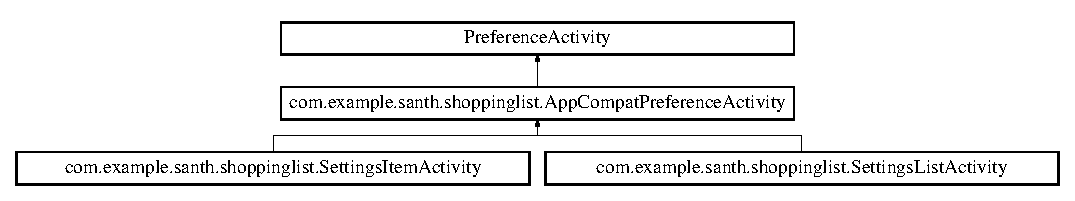
\includegraphics[height=2.258065cm]{classcom_1_1example_1_1santh_1_1shoppinglist_1_1_app_compat_preference_activity}
\end{center}
\end{figure}
\subsection*{Public Member Functions}
\begin{DoxyCompactItemize}
\item 
Action\+Bar \hyperlink{classcom_1_1example_1_1santh_1_1shoppinglist_1_1_app_compat_preference_activity_a91607b20523f10f8c0ad0fd98909dcd6}{get\+Support\+Action\+Bar} ()
\item 
void \hyperlink{classcom_1_1example_1_1santh_1_1shoppinglist_1_1_app_compat_preference_activity_a54367107d69645983c9fd1910aea94b7}{set\+Support\+Action\+Bar} (@Nullable Toolbar toolbar)
\item 
Menu\+Inflater \hyperlink{classcom_1_1example_1_1santh_1_1shoppinglist_1_1_app_compat_preference_activity_a02bbdc41671a52ca45ce63fd79344bd1}{get\+Menu\+Inflater} ()
\item 
void \hyperlink{classcom_1_1example_1_1santh_1_1shoppinglist_1_1_app_compat_preference_activity_a9d021010ecb1f31e868c641dd2a6e6b3}{set\+Content\+View} (@Layout\+Res int layout\+Res\+ID)
\item 
void \hyperlink{classcom_1_1example_1_1santh_1_1shoppinglist_1_1_app_compat_preference_activity_a64f5a742df7b01ab2e792f0a1cbb275f}{set\+Content\+View} (View view)
\item 
void \hyperlink{classcom_1_1example_1_1santh_1_1shoppinglist_1_1_app_compat_preference_activity_a3066cf4e43669fca5248a0b404ec98ae}{set\+Content\+View} (View view, View\+Group.\+Layout\+Params params)
\item 
void \hyperlink{classcom_1_1example_1_1santh_1_1shoppinglist_1_1_app_compat_preference_activity_ac28307936a76730b731bd8f97529f122}{add\+Content\+View} (View view, View\+Group.\+Layout\+Params params)
\item 
void \hyperlink{classcom_1_1example_1_1santh_1_1shoppinglist_1_1_app_compat_preference_activity_a37749d4fd93ceb1d7d00b7343f6985d6}{on\+Configuration\+Changed} (Configuration new\+Config)
\item 
void \hyperlink{classcom_1_1example_1_1santh_1_1shoppinglist_1_1_app_compat_preference_activity_a3dd424e0b20544d1ffb5192120829c20}{invalidate\+Options\+Menu} ()
\end{DoxyCompactItemize}
\subsection*{Protected Member Functions}
\begin{DoxyCompactItemize}
\item 
void \hyperlink{classcom_1_1example_1_1santh_1_1shoppinglist_1_1_app_compat_preference_activity_ad7dc1d3cd1caf48c023cdccb20278f38}{on\+Create} (Bundle saved\+Instance\+State)
\item 
void \hyperlink{classcom_1_1example_1_1santh_1_1shoppinglist_1_1_app_compat_preference_activity_a0c1ac9fcbe62fa6b5cf035fe46300a4b}{on\+Post\+Create} (Bundle saved\+Instance\+State)
\item 
void \hyperlink{classcom_1_1example_1_1santh_1_1shoppinglist_1_1_app_compat_preference_activity_a7bb5ac2ab63490622214ff13dbede839}{on\+Post\+Resume} ()
\item 
void \hyperlink{classcom_1_1example_1_1santh_1_1shoppinglist_1_1_app_compat_preference_activity_ac5fa38dd6673facb57411a7e65870809}{on\+Title\+Changed} (Char\+Sequence title, int color)
\item 
void \hyperlink{classcom_1_1example_1_1santh_1_1shoppinglist_1_1_app_compat_preference_activity_ad4dbca728afaae63f8af58b53a1c31a5}{on\+Stop} ()
\item 
void \hyperlink{classcom_1_1example_1_1santh_1_1shoppinglist_1_1_app_compat_preference_activity_abb6da3f9fb0b275684431b8622945d7c}{on\+Destroy} ()
\end{DoxyCompactItemize}


\subsection{Detailed Description}
A \hyperlink{}{android.\+preference.\+Preference\+Activity} which implements and proxies the necessary calls to be used with App\+Compat. 

\subsection{Member Function Documentation}
\index{com\+::example\+::santh\+::shoppinglist\+::\+App\+Compat\+Preference\+Activity@{com\+::example\+::santh\+::shoppinglist\+::\+App\+Compat\+Preference\+Activity}!add\+Content\+View@{add\+Content\+View}}
\index{add\+Content\+View@{add\+Content\+View}!com\+::example\+::santh\+::shoppinglist\+::\+App\+Compat\+Preference\+Activity@{com\+::example\+::santh\+::shoppinglist\+::\+App\+Compat\+Preference\+Activity}}
\subsubsection[{\texorpdfstring{add\+Content\+View(\+View view, View\+Group.\+Layout\+Params params)}{addContentView(View view, ViewGroup.LayoutParams params)}}]{\setlength{\rightskip}{0pt plus 5cm}void com.\+example.\+santh.\+shoppinglist.\+App\+Compat\+Preference\+Activity.\+add\+Content\+View (
\begin{DoxyParamCaption}
\item[{View}]{view, }
\item[{View\+Group.\+Layout\+Params}]{params}
\end{DoxyParamCaption}
)}\hypertarget{classcom_1_1example_1_1santh_1_1shoppinglist_1_1_app_compat_preference_activity_ac28307936a76730b731bd8f97529f122}{}\label{classcom_1_1example_1_1santh_1_1shoppinglist_1_1_app_compat_preference_activity_ac28307936a76730b731bd8f97529f122}
\index{com\+::example\+::santh\+::shoppinglist\+::\+App\+Compat\+Preference\+Activity@{com\+::example\+::santh\+::shoppinglist\+::\+App\+Compat\+Preference\+Activity}!get\+Menu\+Inflater@{get\+Menu\+Inflater}}
\index{get\+Menu\+Inflater@{get\+Menu\+Inflater}!com\+::example\+::santh\+::shoppinglist\+::\+App\+Compat\+Preference\+Activity@{com\+::example\+::santh\+::shoppinglist\+::\+App\+Compat\+Preference\+Activity}}
\subsubsection[{\texorpdfstring{get\+Menu\+Inflater()}{getMenuInflater()}}]{\setlength{\rightskip}{0pt plus 5cm}Menu\+Inflater com.\+example.\+santh.\+shoppinglist.\+App\+Compat\+Preference\+Activity.\+get\+Menu\+Inflater (
\begin{DoxyParamCaption}
{}
\end{DoxyParamCaption}
)}\hypertarget{classcom_1_1example_1_1santh_1_1shoppinglist_1_1_app_compat_preference_activity_a02bbdc41671a52ca45ce63fd79344bd1}{}\label{classcom_1_1example_1_1santh_1_1shoppinglist_1_1_app_compat_preference_activity_a02bbdc41671a52ca45ce63fd79344bd1}
\index{com\+::example\+::santh\+::shoppinglist\+::\+App\+Compat\+Preference\+Activity@{com\+::example\+::santh\+::shoppinglist\+::\+App\+Compat\+Preference\+Activity}!get\+Support\+Action\+Bar@{get\+Support\+Action\+Bar}}
\index{get\+Support\+Action\+Bar@{get\+Support\+Action\+Bar}!com\+::example\+::santh\+::shoppinglist\+::\+App\+Compat\+Preference\+Activity@{com\+::example\+::santh\+::shoppinglist\+::\+App\+Compat\+Preference\+Activity}}
\subsubsection[{\texorpdfstring{get\+Support\+Action\+Bar()}{getSupportActionBar()}}]{\setlength{\rightskip}{0pt plus 5cm}Action\+Bar com.\+example.\+santh.\+shoppinglist.\+App\+Compat\+Preference\+Activity.\+get\+Support\+Action\+Bar (
\begin{DoxyParamCaption}
{}
\end{DoxyParamCaption}
)}\hypertarget{classcom_1_1example_1_1santh_1_1shoppinglist_1_1_app_compat_preference_activity_a91607b20523f10f8c0ad0fd98909dcd6}{}\label{classcom_1_1example_1_1santh_1_1shoppinglist_1_1_app_compat_preference_activity_a91607b20523f10f8c0ad0fd98909dcd6}
\index{com\+::example\+::santh\+::shoppinglist\+::\+App\+Compat\+Preference\+Activity@{com\+::example\+::santh\+::shoppinglist\+::\+App\+Compat\+Preference\+Activity}!invalidate\+Options\+Menu@{invalidate\+Options\+Menu}}
\index{invalidate\+Options\+Menu@{invalidate\+Options\+Menu}!com\+::example\+::santh\+::shoppinglist\+::\+App\+Compat\+Preference\+Activity@{com\+::example\+::santh\+::shoppinglist\+::\+App\+Compat\+Preference\+Activity}}
\subsubsection[{\texorpdfstring{invalidate\+Options\+Menu()}{invalidateOptionsMenu()}}]{\setlength{\rightskip}{0pt plus 5cm}void com.\+example.\+santh.\+shoppinglist.\+App\+Compat\+Preference\+Activity.\+invalidate\+Options\+Menu (
\begin{DoxyParamCaption}
{}
\end{DoxyParamCaption}
)}\hypertarget{classcom_1_1example_1_1santh_1_1shoppinglist_1_1_app_compat_preference_activity_a3dd424e0b20544d1ffb5192120829c20}{}\label{classcom_1_1example_1_1santh_1_1shoppinglist_1_1_app_compat_preference_activity_a3dd424e0b20544d1ffb5192120829c20}
\index{com\+::example\+::santh\+::shoppinglist\+::\+App\+Compat\+Preference\+Activity@{com\+::example\+::santh\+::shoppinglist\+::\+App\+Compat\+Preference\+Activity}!on\+Configuration\+Changed@{on\+Configuration\+Changed}}
\index{on\+Configuration\+Changed@{on\+Configuration\+Changed}!com\+::example\+::santh\+::shoppinglist\+::\+App\+Compat\+Preference\+Activity@{com\+::example\+::santh\+::shoppinglist\+::\+App\+Compat\+Preference\+Activity}}
\subsubsection[{\texorpdfstring{on\+Configuration\+Changed(\+Configuration new\+Config)}{onConfigurationChanged(Configuration newConfig)}}]{\setlength{\rightskip}{0pt plus 5cm}void com.\+example.\+santh.\+shoppinglist.\+App\+Compat\+Preference\+Activity.\+on\+Configuration\+Changed (
\begin{DoxyParamCaption}
\item[{Configuration}]{new\+Config}
\end{DoxyParamCaption}
)}\hypertarget{classcom_1_1example_1_1santh_1_1shoppinglist_1_1_app_compat_preference_activity_a37749d4fd93ceb1d7d00b7343f6985d6}{}\label{classcom_1_1example_1_1santh_1_1shoppinglist_1_1_app_compat_preference_activity_a37749d4fd93ceb1d7d00b7343f6985d6}
\index{com\+::example\+::santh\+::shoppinglist\+::\+App\+Compat\+Preference\+Activity@{com\+::example\+::santh\+::shoppinglist\+::\+App\+Compat\+Preference\+Activity}!on\+Create@{on\+Create}}
\index{on\+Create@{on\+Create}!com\+::example\+::santh\+::shoppinglist\+::\+App\+Compat\+Preference\+Activity@{com\+::example\+::santh\+::shoppinglist\+::\+App\+Compat\+Preference\+Activity}}
\subsubsection[{\texorpdfstring{on\+Create(\+Bundle saved\+Instance\+State)}{onCreate(Bundle savedInstanceState)}}]{\setlength{\rightskip}{0pt plus 5cm}void com.\+example.\+santh.\+shoppinglist.\+App\+Compat\+Preference\+Activity.\+on\+Create (
\begin{DoxyParamCaption}
\item[{Bundle}]{saved\+Instance\+State}
\end{DoxyParamCaption}
)\hspace{0.3cm}{\ttfamily [protected]}}\hypertarget{classcom_1_1example_1_1santh_1_1shoppinglist_1_1_app_compat_preference_activity_ad7dc1d3cd1caf48c023cdccb20278f38}{}\label{classcom_1_1example_1_1santh_1_1shoppinglist_1_1_app_compat_preference_activity_ad7dc1d3cd1caf48c023cdccb20278f38}
\index{com\+::example\+::santh\+::shoppinglist\+::\+App\+Compat\+Preference\+Activity@{com\+::example\+::santh\+::shoppinglist\+::\+App\+Compat\+Preference\+Activity}!on\+Destroy@{on\+Destroy}}
\index{on\+Destroy@{on\+Destroy}!com\+::example\+::santh\+::shoppinglist\+::\+App\+Compat\+Preference\+Activity@{com\+::example\+::santh\+::shoppinglist\+::\+App\+Compat\+Preference\+Activity}}
\subsubsection[{\texorpdfstring{on\+Destroy()}{onDestroy()}}]{\setlength{\rightskip}{0pt plus 5cm}void com.\+example.\+santh.\+shoppinglist.\+App\+Compat\+Preference\+Activity.\+on\+Destroy (
\begin{DoxyParamCaption}
{}
\end{DoxyParamCaption}
)\hspace{0.3cm}{\ttfamily [protected]}}\hypertarget{classcom_1_1example_1_1santh_1_1shoppinglist_1_1_app_compat_preference_activity_abb6da3f9fb0b275684431b8622945d7c}{}\label{classcom_1_1example_1_1santh_1_1shoppinglist_1_1_app_compat_preference_activity_abb6da3f9fb0b275684431b8622945d7c}
\index{com\+::example\+::santh\+::shoppinglist\+::\+App\+Compat\+Preference\+Activity@{com\+::example\+::santh\+::shoppinglist\+::\+App\+Compat\+Preference\+Activity}!on\+Post\+Create@{on\+Post\+Create}}
\index{on\+Post\+Create@{on\+Post\+Create}!com\+::example\+::santh\+::shoppinglist\+::\+App\+Compat\+Preference\+Activity@{com\+::example\+::santh\+::shoppinglist\+::\+App\+Compat\+Preference\+Activity}}
\subsubsection[{\texorpdfstring{on\+Post\+Create(\+Bundle saved\+Instance\+State)}{onPostCreate(Bundle savedInstanceState)}}]{\setlength{\rightskip}{0pt plus 5cm}void com.\+example.\+santh.\+shoppinglist.\+App\+Compat\+Preference\+Activity.\+on\+Post\+Create (
\begin{DoxyParamCaption}
\item[{Bundle}]{saved\+Instance\+State}
\end{DoxyParamCaption}
)\hspace{0.3cm}{\ttfamily [protected]}}\hypertarget{classcom_1_1example_1_1santh_1_1shoppinglist_1_1_app_compat_preference_activity_a0c1ac9fcbe62fa6b5cf035fe46300a4b}{}\label{classcom_1_1example_1_1santh_1_1shoppinglist_1_1_app_compat_preference_activity_a0c1ac9fcbe62fa6b5cf035fe46300a4b}
\index{com\+::example\+::santh\+::shoppinglist\+::\+App\+Compat\+Preference\+Activity@{com\+::example\+::santh\+::shoppinglist\+::\+App\+Compat\+Preference\+Activity}!on\+Post\+Resume@{on\+Post\+Resume}}
\index{on\+Post\+Resume@{on\+Post\+Resume}!com\+::example\+::santh\+::shoppinglist\+::\+App\+Compat\+Preference\+Activity@{com\+::example\+::santh\+::shoppinglist\+::\+App\+Compat\+Preference\+Activity}}
\subsubsection[{\texorpdfstring{on\+Post\+Resume()}{onPostResume()}}]{\setlength{\rightskip}{0pt plus 5cm}void com.\+example.\+santh.\+shoppinglist.\+App\+Compat\+Preference\+Activity.\+on\+Post\+Resume (
\begin{DoxyParamCaption}
{}
\end{DoxyParamCaption}
)\hspace{0.3cm}{\ttfamily [protected]}}\hypertarget{classcom_1_1example_1_1santh_1_1shoppinglist_1_1_app_compat_preference_activity_a7bb5ac2ab63490622214ff13dbede839}{}\label{classcom_1_1example_1_1santh_1_1shoppinglist_1_1_app_compat_preference_activity_a7bb5ac2ab63490622214ff13dbede839}
\index{com\+::example\+::santh\+::shoppinglist\+::\+App\+Compat\+Preference\+Activity@{com\+::example\+::santh\+::shoppinglist\+::\+App\+Compat\+Preference\+Activity}!on\+Stop@{on\+Stop}}
\index{on\+Stop@{on\+Stop}!com\+::example\+::santh\+::shoppinglist\+::\+App\+Compat\+Preference\+Activity@{com\+::example\+::santh\+::shoppinglist\+::\+App\+Compat\+Preference\+Activity}}
\subsubsection[{\texorpdfstring{on\+Stop()}{onStop()}}]{\setlength{\rightskip}{0pt plus 5cm}void com.\+example.\+santh.\+shoppinglist.\+App\+Compat\+Preference\+Activity.\+on\+Stop (
\begin{DoxyParamCaption}
{}
\end{DoxyParamCaption}
)\hspace{0.3cm}{\ttfamily [protected]}}\hypertarget{classcom_1_1example_1_1santh_1_1shoppinglist_1_1_app_compat_preference_activity_ad4dbca728afaae63f8af58b53a1c31a5}{}\label{classcom_1_1example_1_1santh_1_1shoppinglist_1_1_app_compat_preference_activity_ad4dbca728afaae63f8af58b53a1c31a5}
\index{com\+::example\+::santh\+::shoppinglist\+::\+App\+Compat\+Preference\+Activity@{com\+::example\+::santh\+::shoppinglist\+::\+App\+Compat\+Preference\+Activity}!on\+Title\+Changed@{on\+Title\+Changed}}
\index{on\+Title\+Changed@{on\+Title\+Changed}!com\+::example\+::santh\+::shoppinglist\+::\+App\+Compat\+Preference\+Activity@{com\+::example\+::santh\+::shoppinglist\+::\+App\+Compat\+Preference\+Activity}}
\subsubsection[{\texorpdfstring{on\+Title\+Changed(\+Char\+Sequence title, int color)}{onTitleChanged(CharSequence title, int color)}}]{\setlength{\rightskip}{0pt plus 5cm}void com.\+example.\+santh.\+shoppinglist.\+App\+Compat\+Preference\+Activity.\+on\+Title\+Changed (
\begin{DoxyParamCaption}
\item[{Char\+Sequence}]{title, }
\item[{int}]{color}
\end{DoxyParamCaption}
)\hspace{0.3cm}{\ttfamily [protected]}}\hypertarget{classcom_1_1example_1_1santh_1_1shoppinglist_1_1_app_compat_preference_activity_ac5fa38dd6673facb57411a7e65870809}{}\label{classcom_1_1example_1_1santh_1_1shoppinglist_1_1_app_compat_preference_activity_ac5fa38dd6673facb57411a7e65870809}
\index{com\+::example\+::santh\+::shoppinglist\+::\+App\+Compat\+Preference\+Activity@{com\+::example\+::santh\+::shoppinglist\+::\+App\+Compat\+Preference\+Activity}!set\+Content\+View@{set\+Content\+View}}
\index{set\+Content\+View@{set\+Content\+View}!com\+::example\+::santh\+::shoppinglist\+::\+App\+Compat\+Preference\+Activity@{com\+::example\+::santh\+::shoppinglist\+::\+App\+Compat\+Preference\+Activity}}
\subsubsection[{\texorpdfstring{set\+Content\+View("@Layout\+Res int layout\+Res\+I\+D)}{setContentView(@LayoutRes int layoutResID)}}]{\setlength{\rightskip}{0pt plus 5cm}void com.\+example.\+santh.\+shoppinglist.\+App\+Compat\+Preference\+Activity.\+set\+Content\+View (
\begin{DoxyParamCaption}
\item[{@Layout\+Res int}]{layout\+Res\+ID}
\end{DoxyParamCaption}
)}\hypertarget{classcom_1_1example_1_1santh_1_1shoppinglist_1_1_app_compat_preference_activity_a9d021010ecb1f31e868c641dd2a6e6b3}{}\label{classcom_1_1example_1_1santh_1_1shoppinglist_1_1_app_compat_preference_activity_a9d021010ecb1f31e868c641dd2a6e6b3}
\index{com\+::example\+::santh\+::shoppinglist\+::\+App\+Compat\+Preference\+Activity@{com\+::example\+::santh\+::shoppinglist\+::\+App\+Compat\+Preference\+Activity}!set\+Content\+View@{set\+Content\+View}}
\index{set\+Content\+View@{set\+Content\+View}!com\+::example\+::santh\+::shoppinglist\+::\+App\+Compat\+Preference\+Activity@{com\+::example\+::santh\+::shoppinglist\+::\+App\+Compat\+Preference\+Activity}}
\subsubsection[{\texorpdfstring{set\+Content\+View(\+View view)}{setContentView(View view)}}]{\setlength{\rightskip}{0pt plus 5cm}void com.\+example.\+santh.\+shoppinglist.\+App\+Compat\+Preference\+Activity.\+set\+Content\+View (
\begin{DoxyParamCaption}
\item[{View}]{view}
\end{DoxyParamCaption}
)}\hypertarget{classcom_1_1example_1_1santh_1_1shoppinglist_1_1_app_compat_preference_activity_a64f5a742df7b01ab2e792f0a1cbb275f}{}\label{classcom_1_1example_1_1santh_1_1shoppinglist_1_1_app_compat_preference_activity_a64f5a742df7b01ab2e792f0a1cbb275f}
\index{com\+::example\+::santh\+::shoppinglist\+::\+App\+Compat\+Preference\+Activity@{com\+::example\+::santh\+::shoppinglist\+::\+App\+Compat\+Preference\+Activity}!set\+Content\+View@{set\+Content\+View}}
\index{set\+Content\+View@{set\+Content\+View}!com\+::example\+::santh\+::shoppinglist\+::\+App\+Compat\+Preference\+Activity@{com\+::example\+::santh\+::shoppinglist\+::\+App\+Compat\+Preference\+Activity}}
\subsubsection[{\texorpdfstring{set\+Content\+View(\+View view, View\+Group.\+Layout\+Params params)}{setContentView(View view, ViewGroup.LayoutParams params)}}]{\setlength{\rightskip}{0pt plus 5cm}void com.\+example.\+santh.\+shoppinglist.\+App\+Compat\+Preference\+Activity.\+set\+Content\+View (
\begin{DoxyParamCaption}
\item[{View}]{view, }
\item[{View\+Group.\+Layout\+Params}]{params}
\end{DoxyParamCaption}
)}\hypertarget{classcom_1_1example_1_1santh_1_1shoppinglist_1_1_app_compat_preference_activity_a3066cf4e43669fca5248a0b404ec98ae}{}\label{classcom_1_1example_1_1santh_1_1shoppinglist_1_1_app_compat_preference_activity_a3066cf4e43669fca5248a0b404ec98ae}
\index{com\+::example\+::santh\+::shoppinglist\+::\+App\+Compat\+Preference\+Activity@{com\+::example\+::santh\+::shoppinglist\+::\+App\+Compat\+Preference\+Activity}!set\+Support\+Action\+Bar@{set\+Support\+Action\+Bar}}
\index{set\+Support\+Action\+Bar@{set\+Support\+Action\+Bar}!com\+::example\+::santh\+::shoppinglist\+::\+App\+Compat\+Preference\+Activity@{com\+::example\+::santh\+::shoppinglist\+::\+App\+Compat\+Preference\+Activity}}
\subsubsection[{\texorpdfstring{set\+Support\+Action\+Bar("@Nullable Toolbar toolbar)}{setSupportActionBar(@Nullable Toolbar toolbar)}}]{\setlength{\rightskip}{0pt plus 5cm}void com.\+example.\+santh.\+shoppinglist.\+App\+Compat\+Preference\+Activity.\+set\+Support\+Action\+Bar (
\begin{DoxyParamCaption}
\item[{@Nullable Toolbar}]{toolbar}
\end{DoxyParamCaption}
)}\hypertarget{classcom_1_1example_1_1santh_1_1shoppinglist_1_1_app_compat_preference_activity_a54367107d69645983c9fd1910aea94b7}{}\label{classcom_1_1example_1_1santh_1_1shoppinglist_1_1_app_compat_preference_activity_a54367107d69645983c9fd1910aea94b7}


The documentation for this class was generated from the following file\+:\begin{DoxyCompactItemize}
\item 
E\+:/\+Android/\+Shopping\+List\+D\+B4 2/app/src/main/java/com/example/santh/shoppinglist/\hyperlink{_app_compat_preference_activity_8java}{App\+Compat\+Preference\+Activity.\+java}\end{DoxyCompactItemize}

\hypertarget{classcom_1_1example_1_1santh_1_1shoppinglist_1_1_custom_auto_complete_text_changed_listener}{}\section{com.\+example.\+santh.\+shoppinglist.\+Custom\+Auto\+Complete\+Text\+Changed\+Listener Class Reference}
\label{classcom_1_1example_1_1santh_1_1shoppinglist_1_1_custom_auto_complete_text_changed_listener}\index{com.\+example.\+santh.\+shoppinglist.\+Custom\+Auto\+Complete\+Text\+Changed\+Listener@{com.\+example.\+santh.\+shoppinglist.\+Custom\+Auto\+Complete\+Text\+Changed\+Listener}}


\hyperlink{classcom_1_1example_1_1santh_1_1shoppinglist_1_1_custom_auto_complete_text_changed_listener}{Custom\+Auto\+Complete\+Text\+Changed\+Listener} is used to get the Products from DB when a character has been changed by user.  


Inheritance diagram for com.\+example.\+santh.\+shoppinglist.\+Custom\+Auto\+Complete\+Text\+Changed\+Listener\+:\begin{figure}[H]
\begin{center}
\leavevmode
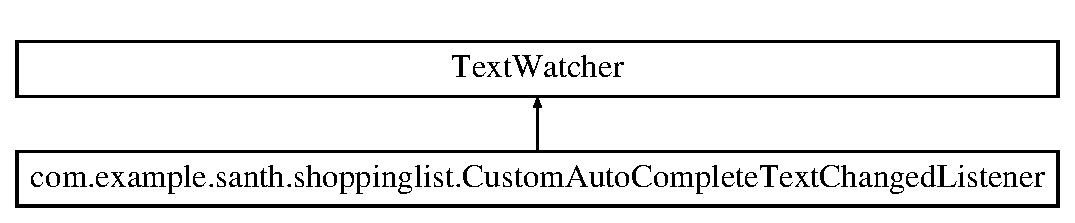
\includegraphics[height=2.000000cm]{classcom_1_1example_1_1santh_1_1shoppinglist_1_1_custom_auto_complete_text_changed_listener}
\end{center}
\end{figure}
\subsection*{Public Member Functions}
\begin{DoxyCompactItemize}
\item 
\hyperlink{classcom_1_1example_1_1santh_1_1shoppinglist_1_1_custom_auto_complete_text_changed_listener_a7bfd44ba7bf1c8efc03affa0141c47d6}{Custom\+Auto\+Complete\+Text\+Changed\+Listener} (Context context)
\item 
void \hyperlink{classcom_1_1example_1_1santh_1_1shoppinglist_1_1_custom_auto_complete_text_changed_listener_aa989a3cebf9d00d6890109bc4af95b4a}{after\+Text\+Changed} (Editable s)
\item 
void \hyperlink{classcom_1_1example_1_1santh_1_1shoppinglist_1_1_custom_auto_complete_text_changed_listener_a21edbf3f7a843071c09e56a99d382f35}{before\+Text\+Changed} (Char\+Sequence s, int start, int count, int after)
\item 
void \hyperlink{classcom_1_1example_1_1santh_1_1shoppinglist_1_1_custom_auto_complete_text_changed_listener_a273187b7db0bec83b92ec9a9b81e6794}{on\+Text\+Changed} (Char\+Sequence user\+Input, int start, int before, int count)
\begin{DoxyCompactList}\small\item\em Text Changed Method is called whenever user enters a new character in autocomplete field. \end{DoxyCompactList}\end{DoxyCompactItemize}
\subsection*{Static Public Attributes}
\begin{DoxyCompactItemize}
\item 
static final String \hyperlink{classcom_1_1example_1_1santh_1_1shoppinglist_1_1_custom_auto_complete_text_changed_listener_a9f6397680811363d2433486f973ca6ff}{T\+AG} = \char`\"{}Custom\+Auto\+Complete\+Text\+Changed\+Listener.\+java\char`\"{}
\end{DoxyCompactItemize}


\subsection{Detailed Description}
\hyperlink{classcom_1_1example_1_1santh_1_1shoppinglist_1_1_custom_auto_complete_text_changed_listener}{Custom\+Auto\+Complete\+Text\+Changed\+Listener} is used to get the Products from DB when a character has been changed by user. 

\subsection{Constructor \& Destructor Documentation}
\index{com\+::example\+::santh\+::shoppinglist\+::\+Custom\+Auto\+Complete\+Text\+Changed\+Listener@{com\+::example\+::santh\+::shoppinglist\+::\+Custom\+Auto\+Complete\+Text\+Changed\+Listener}!Custom\+Auto\+Complete\+Text\+Changed\+Listener@{Custom\+Auto\+Complete\+Text\+Changed\+Listener}}
\index{Custom\+Auto\+Complete\+Text\+Changed\+Listener@{Custom\+Auto\+Complete\+Text\+Changed\+Listener}!com\+::example\+::santh\+::shoppinglist\+::\+Custom\+Auto\+Complete\+Text\+Changed\+Listener@{com\+::example\+::santh\+::shoppinglist\+::\+Custom\+Auto\+Complete\+Text\+Changed\+Listener}}
\subsubsection[{\texorpdfstring{Custom\+Auto\+Complete\+Text\+Changed\+Listener(\+Context context)}{CustomAutoCompleteTextChangedListener(Context context)}}]{\setlength{\rightskip}{0pt plus 5cm}com.\+example.\+santh.\+shoppinglist.\+Custom\+Auto\+Complete\+Text\+Changed\+Listener.\+Custom\+Auto\+Complete\+Text\+Changed\+Listener (
\begin{DoxyParamCaption}
\item[{Context}]{context}
\end{DoxyParamCaption}
)}\hypertarget{classcom_1_1example_1_1santh_1_1shoppinglist_1_1_custom_auto_complete_text_changed_listener_a7bfd44ba7bf1c8efc03affa0141c47d6}{}\label{classcom_1_1example_1_1santh_1_1shoppinglist_1_1_custom_auto_complete_text_changed_listener_a7bfd44ba7bf1c8efc03affa0141c47d6}


\subsection{Member Function Documentation}
\index{com\+::example\+::santh\+::shoppinglist\+::\+Custom\+Auto\+Complete\+Text\+Changed\+Listener@{com\+::example\+::santh\+::shoppinglist\+::\+Custom\+Auto\+Complete\+Text\+Changed\+Listener}!after\+Text\+Changed@{after\+Text\+Changed}}
\index{after\+Text\+Changed@{after\+Text\+Changed}!com\+::example\+::santh\+::shoppinglist\+::\+Custom\+Auto\+Complete\+Text\+Changed\+Listener@{com\+::example\+::santh\+::shoppinglist\+::\+Custom\+Auto\+Complete\+Text\+Changed\+Listener}}
\subsubsection[{\texorpdfstring{after\+Text\+Changed(\+Editable s)}{afterTextChanged(Editable s)}}]{\setlength{\rightskip}{0pt plus 5cm}void com.\+example.\+santh.\+shoppinglist.\+Custom\+Auto\+Complete\+Text\+Changed\+Listener.\+after\+Text\+Changed (
\begin{DoxyParamCaption}
\item[{Editable}]{s}
\end{DoxyParamCaption}
)}\hypertarget{classcom_1_1example_1_1santh_1_1shoppinglist_1_1_custom_auto_complete_text_changed_listener_aa989a3cebf9d00d6890109bc4af95b4a}{}\label{classcom_1_1example_1_1santh_1_1shoppinglist_1_1_custom_auto_complete_text_changed_listener_aa989a3cebf9d00d6890109bc4af95b4a}
\index{com\+::example\+::santh\+::shoppinglist\+::\+Custom\+Auto\+Complete\+Text\+Changed\+Listener@{com\+::example\+::santh\+::shoppinglist\+::\+Custom\+Auto\+Complete\+Text\+Changed\+Listener}!before\+Text\+Changed@{before\+Text\+Changed}}
\index{before\+Text\+Changed@{before\+Text\+Changed}!com\+::example\+::santh\+::shoppinglist\+::\+Custom\+Auto\+Complete\+Text\+Changed\+Listener@{com\+::example\+::santh\+::shoppinglist\+::\+Custom\+Auto\+Complete\+Text\+Changed\+Listener}}
\subsubsection[{\texorpdfstring{before\+Text\+Changed(\+Char\+Sequence s, int start, int count, int after)}{beforeTextChanged(CharSequence s, int start, int count, int after)}}]{\setlength{\rightskip}{0pt plus 5cm}void com.\+example.\+santh.\+shoppinglist.\+Custom\+Auto\+Complete\+Text\+Changed\+Listener.\+before\+Text\+Changed (
\begin{DoxyParamCaption}
\item[{Char\+Sequence}]{s, }
\item[{int}]{start, }
\item[{int}]{count, }
\item[{int}]{after}
\end{DoxyParamCaption}
)}\hypertarget{classcom_1_1example_1_1santh_1_1shoppinglist_1_1_custom_auto_complete_text_changed_listener_a21edbf3f7a843071c09e56a99d382f35}{}\label{classcom_1_1example_1_1santh_1_1shoppinglist_1_1_custom_auto_complete_text_changed_listener_a21edbf3f7a843071c09e56a99d382f35}
\index{com\+::example\+::santh\+::shoppinglist\+::\+Custom\+Auto\+Complete\+Text\+Changed\+Listener@{com\+::example\+::santh\+::shoppinglist\+::\+Custom\+Auto\+Complete\+Text\+Changed\+Listener}!on\+Text\+Changed@{on\+Text\+Changed}}
\index{on\+Text\+Changed@{on\+Text\+Changed}!com\+::example\+::santh\+::shoppinglist\+::\+Custom\+Auto\+Complete\+Text\+Changed\+Listener@{com\+::example\+::santh\+::shoppinglist\+::\+Custom\+Auto\+Complete\+Text\+Changed\+Listener}}
\subsubsection[{\texorpdfstring{on\+Text\+Changed(\+Char\+Sequence user\+Input, int start, int before, int count)}{onTextChanged(CharSequence userInput, int start, int before, int count)}}]{\setlength{\rightskip}{0pt plus 5cm}void com.\+example.\+santh.\+shoppinglist.\+Custom\+Auto\+Complete\+Text\+Changed\+Listener.\+on\+Text\+Changed (
\begin{DoxyParamCaption}
\item[{Char\+Sequence}]{user\+Input, }
\item[{int}]{start, }
\item[{int}]{before, }
\item[{int}]{count}
\end{DoxyParamCaption}
)}\hypertarget{classcom_1_1example_1_1santh_1_1shoppinglist_1_1_custom_auto_complete_text_changed_listener_a273187b7db0bec83b92ec9a9b81e6794}{}\label{classcom_1_1example_1_1santh_1_1shoppinglist_1_1_custom_auto_complete_text_changed_listener_a273187b7db0bec83b92ec9a9b81e6794}


Text Changed Method is called whenever user enters a new character in autocomplete field. 


\begin{DoxyParams}{Parameters}
{\em user\+Input} & \\
\hline
{\em start} & \\
\hline
{\em before} & \\
\hline
{\em count} & \\
\hline
\end{DoxyParams}


\subsection{Member Data Documentation}
\index{com\+::example\+::santh\+::shoppinglist\+::\+Custom\+Auto\+Complete\+Text\+Changed\+Listener@{com\+::example\+::santh\+::shoppinglist\+::\+Custom\+Auto\+Complete\+Text\+Changed\+Listener}!T\+AG@{T\+AG}}
\index{T\+AG@{T\+AG}!com\+::example\+::santh\+::shoppinglist\+::\+Custom\+Auto\+Complete\+Text\+Changed\+Listener@{com\+::example\+::santh\+::shoppinglist\+::\+Custom\+Auto\+Complete\+Text\+Changed\+Listener}}
\subsubsection[{\texorpdfstring{T\+AG}{TAG}}]{\setlength{\rightskip}{0pt plus 5cm}final String com.\+example.\+santh.\+shoppinglist.\+Custom\+Auto\+Complete\+Text\+Changed\+Listener.\+T\+AG = \char`\"{}Custom\+Auto\+Complete\+Text\+Changed\+Listener.\+java\char`\"{}\hspace{0.3cm}{\ttfamily [static]}}\hypertarget{classcom_1_1example_1_1santh_1_1shoppinglist_1_1_custom_auto_complete_text_changed_listener_a9f6397680811363d2433486f973ca6ff}{}\label{classcom_1_1example_1_1santh_1_1shoppinglist_1_1_custom_auto_complete_text_changed_listener_a9f6397680811363d2433486f973ca6ff}


The documentation for this class was generated from the following file\+:\begin{DoxyCompactItemize}
\item 
E\+:/\+Android/\+Shopping\+List\+D\+B4 2/app/src/main/java/com/example/santh/shoppinglist/\hyperlink{_custom_auto_complete_text_changed_listener_8java}{Custom\+Auto\+Complete\+Text\+Changed\+Listener.\+java}\end{DoxyCompactItemize}

\hypertarget{classcom_1_1example_1_1santh_1_1shoppinglist_1_1_custom_auto_complete_view}{}\section{com.\+example.\+santh.\+shoppinglist.\+Custom\+Auto\+Complete\+View Class Reference}
\label{classcom_1_1example_1_1santh_1_1shoppinglist_1_1_custom_auto_complete_view}\index{com.\+example.\+santh.\+shoppinglist.\+Custom\+Auto\+Complete\+View@{com.\+example.\+santh.\+shoppinglist.\+Custom\+Auto\+Complete\+View}}


Cutsom\+Auto\+Complete\+View takes the text entered in the field and shows the matching products suggestions to users.  


Inheritance diagram for com.\+example.\+santh.\+shoppinglist.\+Custom\+Auto\+Complete\+View\+:\begin{figure}[H]
\begin{center}
\leavevmode
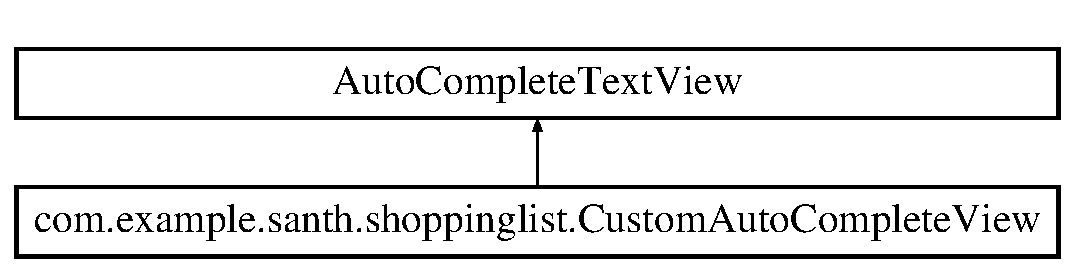
\includegraphics[height=2.000000cm]{classcom_1_1example_1_1santh_1_1shoppinglist_1_1_custom_auto_complete_view}
\end{center}
\end{figure}
\subsection*{Public Member Functions}
\begin{DoxyCompactItemize}
\item 
\hyperlink{classcom_1_1example_1_1santh_1_1shoppinglist_1_1_custom_auto_complete_view_aa4dbe321c154d928530b3c08f931e8cd}{Custom\+Auto\+Complete\+View} (Context context)
\item 
\hyperlink{classcom_1_1example_1_1santh_1_1shoppinglist_1_1_custom_auto_complete_view_a9136c0f8789e4085af0d6cad15c3ed6d}{Custom\+Auto\+Complete\+View} (Context context, Attribute\+Set attrs)
\item 
\hyperlink{classcom_1_1example_1_1santh_1_1shoppinglist_1_1_custom_auto_complete_view_a324556a349a08742220c61ab608904fd}{Custom\+Auto\+Complete\+View} (Context context, Attribute\+Set attrs, int def\+Style)
\end{DoxyCompactItemize}
\subsection*{Protected Member Functions}
\begin{DoxyCompactItemize}
\item 
void \hyperlink{classcom_1_1example_1_1santh_1_1shoppinglist_1_1_custom_auto_complete_view_a92656a23380f4872a86ffdebc135ddb0}{perform\+Filtering} (final Char\+Sequence text, final int key\+Code)
\item 
void \hyperlink{classcom_1_1example_1_1santh_1_1shoppinglist_1_1_custom_auto_complete_view_a9a2d10817c0c2db0ea5ca2f3daa2b14e}{replace\+Text} (final Char\+Sequence text)
\end{DoxyCompactItemize}


\subsection{Detailed Description}
Cutsom\+Auto\+Complete\+View takes the text entered in the field and shows the matching products suggestions to users. 

\subsection{Constructor \& Destructor Documentation}
\index{com\+::example\+::santh\+::shoppinglist\+::\+Custom\+Auto\+Complete\+View@{com\+::example\+::santh\+::shoppinglist\+::\+Custom\+Auto\+Complete\+View}!Custom\+Auto\+Complete\+View@{Custom\+Auto\+Complete\+View}}
\index{Custom\+Auto\+Complete\+View@{Custom\+Auto\+Complete\+View}!com\+::example\+::santh\+::shoppinglist\+::\+Custom\+Auto\+Complete\+View@{com\+::example\+::santh\+::shoppinglist\+::\+Custom\+Auto\+Complete\+View}}
\subsubsection[{\texorpdfstring{Custom\+Auto\+Complete\+View(\+Context context)}{CustomAutoCompleteView(Context context)}}]{\setlength{\rightskip}{0pt plus 5cm}com.\+example.\+santh.\+shoppinglist.\+Custom\+Auto\+Complete\+View.\+Custom\+Auto\+Complete\+View (
\begin{DoxyParamCaption}
\item[{Context}]{context}
\end{DoxyParamCaption}
)}\hypertarget{classcom_1_1example_1_1santh_1_1shoppinglist_1_1_custom_auto_complete_view_aa4dbe321c154d928530b3c08f931e8cd}{}\label{classcom_1_1example_1_1santh_1_1shoppinglist_1_1_custom_auto_complete_view_aa4dbe321c154d928530b3c08f931e8cd}
\index{com\+::example\+::santh\+::shoppinglist\+::\+Custom\+Auto\+Complete\+View@{com\+::example\+::santh\+::shoppinglist\+::\+Custom\+Auto\+Complete\+View}!Custom\+Auto\+Complete\+View@{Custom\+Auto\+Complete\+View}}
\index{Custom\+Auto\+Complete\+View@{Custom\+Auto\+Complete\+View}!com\+::example\+::santh\+::shoppinglist\+::\+Custom\+Auto\+Complete\+View@{com\+::example\+::santh\+::shoppinglist\+::\+Custom\+Auto\+Complete\+View}}
\subsubsection[{\texorpdfstring{Custom\+Auto\+Complete\+View(\+Context context, Attribute\+Set attrs)}{CustomAutoCompleteView(Context context, AttributeSet attrs)}}]{\setlength{\rightskip}{0pt plus 5cm}com.\+example.\+santh.\+shoppinglist.\+Custom\+Auto\+Complete\+View.\+Custom\+Auto\+Complete\+View (
\begin{DoxyParamCaption}
\item[{Context}]{context, }
\item[{Attribute\+Set}]{attrs}
\end{DoxyParamCaption}
)}\hypertarget{classcom_1_1example_1_1santh_1_1shoppinglist_1_1_custom_auto_complete_view_a9136c0f8789e4085af0d6cad15c3ed6d}{}\label{classcom_1_1example_1_1santh_1_1shoppinglist_1_1_custom_auto_complete_view_a9136c0f8789e4085af0d6cad15c3ed6d}
\index{com\+::example\+::santh\+::shoppinglist\+::\+Custom\+Auto\+Complete\+View@{com\+::example\+::santh\+::shoppinglist\+::\+Custom\+Auto\+Complete\+View}!Custom\+Auto\+Complete\+View@{Custom\+Auto\+Complete\+View}}
\index{Custom\+Auto\+Complete\+View@{Custom\+Auto\+Complete\+View}!com\+::example\+::santh\+::shoppinglist\+::\+Custom\+Auto\+Complete\+View@{com\+::example\+::santh\+::shoppinglist\+::\+Custom\+Auto\+Complete\+View}}
\subsubsection[{\texorpdfstring{Custom\+Auto\+Complete\+View(\+Context context, Attribute\+Set attrs, int def\+Style)}{CustomAutoCompleteView(Context context, AttributeSet attrs, int defStyle)}}]{\setlength{\rightskip}{0pt plus 5cm}com.\+example.\+santh.\+shoppinglist.\+Custom\+Auto\+Complete\+View.\+Custom\+Auto\+Complete\+View (
\begin{DoxyParamCaption}
\item[{Context}]{context, }
\item[{Attribute\+Set}]{attrs, }
\item[{int}]{def\+Style}
\end{DoxyParamCaption}
)}\hypertarget{classcom_1_1example_1_1santh_1_1shoppinglist_1_1_custom_auto_complete_view_a324556a349a08742220c61ab608904fd}{}\label{classcom_1_1example_1_1santh_1_1shoppinglist_1_1_custom_auto_complete_view_a324556a349a08742220c61ab608904fd}


\subsection{Member Function Documentation}
\index{com\+::example\+::santh\+::shoppinglist\+::\+Custom\+Auto\+Complete\+View@{com\+::example\+::santh\+::shoppinglist\+::\+Custom\+Auto\+Complete\+View}!perform\+Filtering@{perform\+Filtering}}
\index{perform\+Filtering@{perform\+Filtering}!com\+::example\+::santh\+::shoppinglist\+::\+Custom\+Auto\+Complete\+View@{com\+::example\+::santh\+::shoppinglist\+::\+Custom\+Auto\+Complete\+View}}
\subsubsection[{\texorpdfstring{perform\+Filtering(final Char\+Sequence text, final int key\+Code)}{performFiltering(final CharSequence text, final int keyCode)}}]{\setlength{\rightskip}{0pt plus 5cm}void com.\+example.\+santh.\+shoppinglist.\+Custom\+Auto\+Complete\+View.\+perform\+Filtering (
\begin{DoxyParamCaption}
\item[{final Char\+Sequence}]{text, }
\item[{final int}]{key\+Code}
\end{DoxyParamCaption}
)\hspace{0.3cm}{\ttfamily [protected]}}\hypertarget{classcom_1_1example_1_1santh_1_1shoppinglist_1_1_custom_auto_complete_view_a92656a23380f4872a86ffdebc135ddb0}{}\label{classcom_1_1example_1_1santh_1_1shoppinglist_1_1_custom_auto_complete_view_a92656a23380f4872a86ffdebc135ddb0}
\index{com\+::example\+::santh\+::shoppinglist\+::\+Custom\+Auto\+Complete\+View@{com\+::example\+::santh\+::shoppinglist\+::\+Custom\+Auto\+Complete\+View}!replace\+Text@{replace\+Text}}
\index{replace\+Text@{replace\+Text}!com\+::example\+::santh\+::shoppinglist\+::\+Custom\+Auto\+Complete\+View@{com\+::example\+::santh\+::shoppinglist\+::\+Custom\+Auto\+Complete\+View}}
\subsubsection[{\texorpdfstring{replace\+Text(final Char\+Sequence text)}{replaceText(final CharSequence text)}}]{\setlength{\rightskip}{0pt plus 5cm}void com.\+example.\+santh.\+shoppinglist.\+Custom\+Auto\+Complete\+View.\+replace\+Text (
\begin{DoxyParamCaption}
\item[{final Char\+Sequence}]{text}
\end{DoxyParamCaption}
)\hspace{0.3cm}{\ttfamily [protected]}}\hypertarget{classcom_1_1example_1_1santh_1_1shoppinglist_1_1_custom_auto_complete_view_a9a2d10817c0c2db0ea5ca2f3daa2b14e}{}\label{classcom_1_1example_1_1santh_1_1shoppinglist_1_1_custom_auto_complete_view_a9a2d10817c0c2db0ea5ca2f3daa2b14e}


The documentation for this class was generated from the following file\+:\begin{DoxyCompactItemize}
\item 
E\+:/\+Android/\+Shopping\+List\+D\+B4 2/app/src/main/java/com/example/santh/shoppinglist/\hyperlink{_custom_auto_complete_view_8java}{Custom\+Auto\+Complete\+View.\+java}\end{DoxyCompactItemize}

\hypertarget{classcom_1_1example_1_1santh_1_1shoppinglist_1_1_data_base_manager}{}\section{com.\+example.\+santh.\+shoppinglist.\+Data\+Base\+Manager Class Reference}
\label{classcom_1_1example_1_1santh_1_1shoppinglist_1_1_data_base_manager}\index{com.\+example.\+santh.\+shoppinglist.\+Data\+Base\+Manager@{com.\+example.\+santh.\+shoppinglist.\+Data\+Base\+Manager}}


\hyperlink{classcom_1_1example_1_1santh_1_1shoppinglist_1_1_data_base_manager}{Data\+Base\+Manager} class file to edit delete update and query the database.  


\subsection*{Public Member Functions}
\begin{DoxyCompactItemize}
\item 
\hyperlink{classcom_1_1example_1_1santh_1_1shoppinglist_1_1_data_base_manager_a794167dc3d55c445b8e0f96a50a2f570}{Data\+Base\+Manager} (Context ctx)
\item 
\hyperlink{classcom_1_1example_1_1santh_1_1shoppinglist_1_1_data_base_manager}{Data\+Base\+Manager} \hyperlink{classcom_1_1example_1_1santh_1_1shoppinglist_1_1_data_base_manager_a15cb7f87bbd79a28317ec8079cad963c}{open} ()  throws S\+Q\+L\+Exception 
\item 
void \hyperlink{classcom_1_1example_1_1santh_1_1shoppinglist_1_1_data_base_manager_af981f3e0544fdd6ea19850a0726fbc16}{close} ()
\item 
String \hyperlink{classcom_1_1example_1_1santh_1_1shoppinglist_1_1_data_base_manager_a57ca116807f9a1712924ff51b5c524b7}{get\+Update} ()
\item 
void \hyperlink{classcom_1_1example_1_1santh_1_1shoppinglist_1_1_data_base_manager_a162a3013d5e24320bbcecda77245ab64}{increment\+Update} ()
\item 
void \hyperlink{classcom_1_1example_1_1santh_1_1shoppinglist_1_1_data_base_manager_afe09b80b8a6f0caa804c329738b39163}{add\+Items} (String id, String\mbox{[}$\,$\mbox{]} values)
\item 
J\+S\+O\+N\+Array \hyperlink{classcom_1_1example_1_1santh_1_1shoppinglist_1_1_data_base_manager_a906eed7209379bd1829f268a99c38f21}{compose\+Item\+J\+S\+O\+Nfrom\+S\+Q\+Lite} ()
\begin{DoxyCompactList}\small\item\em Compose J\+S\+ON out of S\+Q\+Lite records. \end{DoxyCompactList}\item 
String \hyperlink{classcom_1_1example_1_1santh_1_1shoppinglist_1_1_data_base_manager_a2906a3cfcc6af2afa4d0448ef15b3b1c}{get\+Item\+Sync\+Status} ()
\begin{DoxyCompactList}\small\item\em Get Sync status of S\+Q\+Lite. \end{DoxyCompactList}\item 
int \hyperlink{classcom_1_1example_1_1santh_1_1shoppinglist_1_1_data_base_manager_ace7f807903efc4baedf52d82144a6999}{db\+Item\+Sync\+Count} ()
\begin{DoxyCompactList}\small\item\em Get S\+Q\+Lite records that are yet to be Synced. \end{DoxyCompactList}\item 
void \hyperlink{classcom_1_1example_1_1santh_1_1shoppinglist_1_1_data_base_manager_a3889f14556813bab328222f9c8831446}{updateitem\+Sync\+Status} ()
\begin{DoxyCompactList}\small\item\em Update Sync status against each User ID. \end{DoxyCompactList}\item 
J\+S\+O\+N\+Array \hyperlink{classcom_1_1example_1_1santh_1_1shoppinglist_1_1_data_base_manager_aaf8610923f0af477c21e8d9fcc8fc17d}{compose\+List\+J\+S\+O\+Nfrom\+S\+Q\+Lite} ()
\begin{DoxyCompactList}\small\item\em Compose J\+S\+ON out of S\+Q\+Lite records. \end{DoxyCompactList}\item 
String \hyperlink{classcom_1_1example_1_1santh_1_1shoppinglist_1_1_data_base_manager_a0a5bc82b127a787eac73dbd6227bdb11}{get\+Sync\+Status} ()
\begin{DoxyCompactList}\small\item\em Get Sync status of S\+Q\+Lite. \end{DoxyCompactList}\item 
int \hyperlink{classcom_1_1example_1_1santh_1_1shoppinglist_1_1_data_base_manager_a4c35804ddfcd4f4308c26329f7d0bfeb}{db\+Sync\+Count} ()
\begin{DoxyCompactList}\small\item\em Get S\+Q\+Lite records that are yet to be Synced. \end{DoxyCompactList}\item 
void \hyperlink{classcom_1_1example_1_1santh_1_1shoppinglist_1_1_data_base_manager_a6ce5935808f974585790c32b68a0da2f}{updatelist\+Sync\+Status} ()
\begin{DoxyCompactList}\small\item\em Update Sync status against each User ID. \end{DoxyCompactList}\item 
void \hyperlink{classcom_1_1example_1_1santh_1_1shoppinglist_1_1_data_base_manager_a5d8ff9c9206acc5cc8aa5b16919a612b}{addcategories} (String id, String\mbox{[}$\,$\mbox{]} values)
\item 
void \hyperlink{classcom_1_1example_1_1santh_1_1shoppinglist_1_1_data_base_manager_a48833dce90f84310f3aefc22d15d7901}{addunits} (String id, String\mbox{[}$\,$\mbox{]} values)
\item 
Cursor \hyperlink{classcom_1_1example_1_1santh_1_1shoppinglist_1_1_data_base_manager_a1c523a8b86965b84704dd916910890d0}{get\+Price} (int ID)
\item 
boolean \hyperlink{classcom_1_1example_1_1santh_1_1shoppinglist_1_1_data_base_manager_a471dab48ad6de705ae874d0b22335de3}{Update\+Data\+Item} (String Item\+Name, int List\+ID, int unitid, int categoryid, String Comments, float Quantity, float Price, int id)
\item 
void \hyperlink{classcom_1_1example_1_1santh_1_1shoppinglist_1_1_data_base_manager_ae539ad8cc244d4da2b60f23d1601b42e}{add\+List} (String id, String\mbox{[}$\,$\mbox{]} values)
\item 
void \hyperlink{classcom_1_1example_1_1santh_1_1shoppinglist_1_1_data_base_manager_ab5aaf1da6ce563dcc4ce4e7f63bc58de}{deletelistid} (String id)
\item 
void \hyperlink{classcom_1_1example_1_1santh_1_1shoppinglist_1_1_data_base_manager_a1e0bad58bdfe608855e3785f82c38d46}{deletecategoryid} (String id)
\item 
void \hyperlink{classcom_1_1example_1_1santh_1_1shoppinglist_1_1_data_base_manager_a987e069d2da99af080009eae9bed0cbe}{deleteunitid} (String id)
\item 
boolean \hyperlink{classcom_1_1example_1_1santh_1_1shoppinglist_1_1_data_base_manager_a69d01cf1de4f01774078111e0eaef829}{insert\+Data\+List} (String List\+Name)
\begin{DoxyCompactList}\small\item\em Insert Function to insert values into table List. \end{DoxyCompactList}\item 
Cursor \hyperlink{classcom_1_1example_1_1santh_1_1shoppinglist_1_1_data_base_manager_afb695f603f9d2f7e58c3746e535358ec}{share\+Listdata} (int List\+Id)
\begin{DoxyCompactList}\small\item\em get all the items and qunatitites to share the list through whatsapp and Email \end{DoxyCompactList}\item 
List$<$ String $>$ \hyperlink{classcom_1_1example_1_1santh_1_1shoppinglist_1_1_data_base_manager_a307e4d523baab740e4e01178d6bd5118}{read} (String Search\+Term)
\begin{DoxyCompactList}\small\item\em Method to get the product suggestions on text changed. \end{DoxyCompactList}\item 
boolean \hyperlink{classcom_1_1example_1_1santh_1_1shoppinglist_1_1_data_base_manager_ae97008248a1324d0eaf6451ac238acaa}{insert\+Data\+Item} (String Item\+Name, int List\+ID, int unitid, int categoryid, String Comments, float Quantity, float Price, int purchased)
\begin{DoxyCompactList}\small\item\em insert\+Data\+Item inserts dataitem to List \end{DoxyCompactList}\item 
Cursor \hyperlink{classcom_1_1example_1_1santh_1_1shoppinglist_1_1_data_base_manager_acd3ba4e19bc7373d4a5f8a307d5c8033}{get\+List\+ID} (String List\+Name)
\item 
Cursor \hyperlink{classcom_1_1example_1_1santh_1_1shoppinglist_1_1_data_base_manager_aa0c1294c6cfc190e00ea11cd6ce6e7ab}{get\+Data\+Item} (int ID)
\begin{DoxyCompactList}\small\item\em Cursor to retrieve data Items. \end{DoxyCompactList}\item 
Cursor \hyperlink{classcom_1_1example_1_1santh_1_1shoppinglist_1_1_data_base_manager_ae4d9ebaa83b3f8503be7b61934bede1b}{get\+Data\+Item\+Cursor} (int ID)
\begin{DoxyCompactList}\small\item\em Cursor to retrieve data Items. \end{DoxyCompactList}\item 
int \hyperlink{classcom_1_1example_1_1santh_1_1shoppinglist_1_1_data_base_manager_aab89b395809febbaf076df571682e57c}{delete\+All} ()
\begin{DoxyCompactList}\small\item\em Delete all records in table. \end{DoxyCompactList}\item 
int \hyperlink{classcom_1_1example_1_1santh_1_1shoppinglist_1_1_data_base_manager_a7273944c8c66bc00f49917270c416b10}{delete\+Items} (int id)
\begin{DoxyCompactList}\small\item\em Delete all items in the List. \end{DoxyCompactList}\item 
int \hyperlink{classcom_1_1example_1_1santh_1_1shoppinglist_1_1_data_base_manager_a74cfb98b2cca130b443a125cdcbc23f5}{delete\+Purchased\+Items} (int id)
\begin{DoxyCompactList}\small\item\em Delete all Purchased Items. \end{DoxyCompactList}\item 
Integer \hyperlink{classcom_1_1example_1_1santh_1_1shoppinglist_1_1_data_base_manager_af44b7c8015d708dd893d208d1abd17a9}{delete\+\_\+\+Itemby\+ID} (int id)
\begin{DoxyCompactList}\small\item\em Delete by ID in Table. \end{DoxyCompactList}\item 
Integer \hyperlink{classcom_1_1example_1_1santh_1_1shoppinglist_1_1_data_base_manager_a9d3b7935c938547342a5901f7b36f525}{delete\+\_\+\+Listby\+ID} (int id)
\begin{DoxyCompactList}\small\item\em Delete List by ID. \end{DoxyCompactList}\item 
boolean \hyperlink{classcom_1_1example_1_1santh_1_1shoppinglist_1_1_data_base_manager_a68c423e2ef83ec63f0836f62637794fe}{updatedata} (String itemname, String original)
\begin{DoxyCompactList}\small\item\em Update Item\+Name in Database. \end{DoxyCompactList}\item 
boolean \hyperlink{classcom_1_1example_1_1santh_1_1shoppinglist_1_1_data_base_manager_a0d54793ae4494224e8c80bb69dd03ae1}{update\+Listdata} (String itemname, String original)
\begin{DoxyCompactList}\small\item\em Update List Name. \end{DoxyCompactList}\item 
boolean \hyperlink{classcom_1_1example_1_1santh_1_1shoppinglist_1_1_data_base_manager_acc9756c58ed8994133dff1241a62f896}{update\+Item\+Purchased} (int id1)
\begin{DoxyCompactList}\small\item\em Update Item as Purchased. \end{DoxyCompactList}\item 
boolean \hyperlink{classcom_1_1example_1_1santh_1_1shoppinglist_1_1_data_base_manager_a14844033da2d6593a848a377a21d96a3}{update\+Item\+Not\+Purchased} (int id1)
\begin{DoxyCompactList}\small\item\em Update Item as Not purchased. \end{DoxyCompactList}\item 
Cursor \hyperlink{classcom_1_1example_1_1santh_1_1shoppinglist_1_1_data_base_manager_a22a3d9161c068013b59434ce07511985}{sortdata} (int Id)
\begin{DoxyCompactList}\small\item\em Sort\+Data to arrange items in list. \end{DoxyCompactList}\item 
Cursor \hyperlink{classcom_1_1example_1_1santh_1_1shoppinglist_1_1_data_base_manager_a9b0d6f7aeea8ec2126210a3ab0f15bad}{sortcategory} (int Id)
\begin{DoxyCompactList}\small\item\em Sort Items By Category. \end{DoxyCompactList}\item 
Cursor \hyperlink{classcom_1_1example_1_1santh_1_1shoppinglist_1_1_data_base_manager_afdb5f5c276c4111164a9c261d040a64d}{sortshowall} (int Id)
\item 
Cursor \hyperlink{classcom_1_1example_1_1santh_1_1shoppinglist_1_1_data_base_manager_aabf476fd3269890f86e97eb7948c95c4}{sortshow010} (int Id)
\item 
Cursor \hyperlink{classcom_1_1example_1_1santh_1_1shoppinglist_1_1_data_base_manager_abbf59fb07c43e403b0a231d9be6f6ad4}{sortshow100} (int Id)
\item 
Cursor \hyperlink{classcom_1_1example_1_1santh_1_1shoppinglist_1_1_data_base_manager_a26442de7ea4e3da9f5a57fb1005b063b}{sortshow110} (int Id)
\item 
void \hyperlink{classcom_1_1example_1_1santh_1_1shoppinglist_1_1_data_base_manager_a968efcc4a15cd2582dbb46253c67fa96}{strikeallitems} (int id)
\item 
void \hyperlink{classcom_1_1example_1_1santh_1_1shoppinglist_1_1_data_base_manager_a6097146d423c0c705e7405c542b17783}{unstrikeallitems} (int id)
\item 
Cursor \hyperlink{classcom_1_1example_1_1santh_1_1shoppinglist_1_1_data_base_manager_a3b63b54bc23f0a06749e710cde064995}{sortcategorydata} (int Id)
\item 
Cursor \hyperlink{classcom_1_1example_1_1santh_1_1shoppinglist_1_1_data_base_manager_ac00576993fafdc4d77e7794a351d7365}{sort\+Lists} ()
\begin{DoxyCompactList}\small\item\em Sort Lists Alphabetically. \end{DoxyCompactList}\item 
Cursor \hyperlink{classcom_1_1example_1_1santh_1_1shoppinglist_1_1_data_base_manager_a7a587023ac7dcef1569da63b6cbf4d66}{sort\+Lists\+Price} ()
\item 
Cursor \hyperlink{classcom_1_1example_1_1santh_1_1shoppinglist_1_1_data_base_manager_ae1cac16a081cbd3ed3fc0dded7c3d306}{sort\+Lists\+Price\+Alpha} ()
\item 
Cursor \hyperlink{classcom_1_1example_1_1santh_1_1shoppinglist_1_1_data_base_manager_a34cecc0ce7f84fe53cddad15284a892b}{get\+Purchased\+List} (int id)
\begin{DoxyCompactList}\small\item\em Get Count of items Purchased in the List. \end{DoxyCompactList}\item 
Cursor \hyperlink{classcom_1_1example_1_1santh_1_1shoppinglist_1_1_data_base_manager_ae9646927170d242e1727f5be44778b04}{get\+Un\+Purchased\+List} (int id)
\begin{DoxyCompactList}\small\item\em Get Count of Items which are not Yet Purchased. \end{DoxyCompactList}\item 
boolean \hyperlink{classcom_1_1example_1_1santh_1_1shoppinglist_1_1_data_base_manager_a84ee149222f9b8c6aeff90904db86df8}{checkdata} (String item\+Name, int id)
\begin{DoxyCompactList}\small\item\em Check\+If\+Dataitem Exists. \end{DoxyCompactList}\item 
boolean \hyperlink{classcom_1_1example_1_1santh_1_1shoppinglist_1_1_data_base_manager_a56a7c1db72d0a27b31bd26facae87bc0}{check\+Listdata} (String item\+Name)
\begin{DoxyCompactList}\small\item\em Check if a List Name Exists. \end{DoxyCompactList}\item 
Cursor \hyperlink{classcom_1_1example_1_1santh_1_1shoppinglist_1_1_data_base_manager_a481240bf420f4e57240eee75c396f034}{get\+Lists} ()
\begin{DoxyCompactList}\small\item\em get all List Names \end{DoxyCompactList}\item 
List$<$ String $>$ \hyperlink{classcom_1_1example_1_1santh_1_1shoppinglist_1_1_data_base_manager_ad88a038d25f0248937118787296a76ba}{get\+Units} ()
\begin{DoxyCompactList}\small\item\em Get all Units. \end{DoxyCompactList}\item 
Cursor \hyperlink{classcom_1_1example_1_1santh_1_1shoppinglist_1_1_data_base_manager_abdc53399fddf45780c6982c500a87cb2}{getunitname} (int unitid)
\item 
Cursor \hyperlink{classcom_1_1example_1_1santh_1_1shoppinglist_1_1_data_base_manager_a42642480f4b6994d40939638eb9348e8}{getcategoryname} (int categoryid)
\item 
Cursor \hyperlink{classcom_1_1example_1_1santh_1_1shoppinglist_1_1_data_base_manager_a24c43da6384cbe3a244f30d9583011fa}{getunitid} (String unitname)
\item 
Cursor \hyperlink{classcom_1_1example_1_1santh_1_1shoppinglist_1_1_data_base_manager_a85b785ca8012c85c5fc1ccb548b361fd}{getcategoryid} (String categoryname)
\item 
List$<$ String $>$ \hyperlink{classcom_1_1example_1_1santh_1_1shoppinglist_1_1_data_base_manager_a3e0f1f4eeebc8f8fa50fd3a978b3ec21}{get\+Category} ()
\begin{DoxyCompactList}\small\item\em Get all categories. \end{DoxyCompactList}\item 
Cursor \hyperlink{classcom_1_1example_1_1santh_1_1shoppinglist_1_1_data_base_manager_a53d1ac0f496bbb3e4e7f8ff35ff6f159}{get\+Item\+Details} (int ID)
\begin{DoxyCompactList}\small\item\em Get all Item Details. \end{DoxyCompactList}\end{DoxyCompactItemize}
\subsection*{Static Public Attributes}
\begin{DoxyCompactItemize}
\item 
static final int \hyperlink{classcom_1_1example_1_1santh_1_1shoppinglist_1_1_data_base_manager_a390eab428a5fa43c2a986cc0396800dc}{D\+A\+T\+A\+B\+A\+S\+E\+\_\+\+V\+E\+R\+S\+I\+ON} = 1
\item 
static final String \hyperlink{classcom_1_1example_1_1santh_1_1shoppinglist_1_1_data_base_manager_a715ae8e63c4b8b71d5ee7f84624457b6}{D\+A\+T\+A\+B\+A\+S\+E\+\_\+\+N\+A\+ME} = \char`\"{}Shopping\+List.\+db\char`\"{}
\item 
static final String \hyperlink{classcom_1_1example_1_1santh_1_1shoppinglist_1_1_data_base_manager_a4baaaa98454321bf218711bd5c716dfb}{T\+A\+B\+L\+E\+\_\+\+N\+A\+M\+E\+\_\+\+L\+I\+ST} = \char`\"{}List\char`\"{}
\item 
static final String \hyperlink{classcom_1_1example_1_1santh_1_1shoppinglist_1_1_data_base_manager_a6001c0b58adbe34cf48abe6c06ee2704}{T\+A\+B\+L\+E\+\_\+\+N\+A\+M\+E\+\_\+\+U\+N\+IT} = \char`\"{}Unit\char`\"{}
\item 
static final String \hyperlink{classcom_1_1example_1_1santh_1_1shoppinglist_1_1_data_base_manager_a93a7ddc84d39f7aacf052122683e8dcf}{T\+A\+B\+L\+E\+\_\+\+N\+A\+M\+E\+\_\+\+C\+A\+T\+E\+G\+O\+RY} = \char`\"{}Category\char`\"{}
\item 
static final String \hyperlink{classcom_1_1example_1_1santh_1_1shoppinglist_1_1_data_base_manager_adef1e883e70f7425117fade0cf0e95c0}{C\+O\+L\+U\+M\+N\+\_\+\+N\+A\+M\+E\+\_\+\+L\+I\+S\+T\+ID} = \char`\"{}listid\char`\"{}
\item 
static final String \hyperlink{classcom_1_1example_1_1santh_1_1shoppinglist_1_1_data_base_manager_ac4fd55b0cb41d7cd67ec2e77d916336c}{C\+O\+L\+U\+M\+N\+\_\+\+N\+A\+M\+E\+\_\+\+L\+I\+S\+T\+N\+A\+ME} = \char`\"{}listname\char`\"{}
\item 
static final String \hyperlink{classcom_1_1example_1_1santh_1_1shoppinglist_1_1_data_base_manager_a76d9454b49ce6a5f120990df1e0a4338}{T\+A\+B\+L\+E\+\_\+\+N\+A\+M\+E\+\_\+\+I\+T\+EM} = \char`\"{}Item\char`\"{}
\item 
static final String \hyperlink{classcom_1_1example_1_1santh_1_1shoppinglist_1_1_data_base_manager_a9e8a8e983956f2de8440c37a7a6b378a}{C\+O\+L\+U\+M\+N\+\_\+\+N\+A\+M\+E\+\_\+\+I\+T\+E\+M\+\_\+\+ID} = \char`\"{}itemid\char`\"{}
\item 
static final String \hyperlink{classcom_1_1example_1_1santh_1_1shoppinglist_1_1_data_base_manager_a9b6b0327269905ec57c1be48ed26d5ce}{C\+O\+L\+U\+M\+N\+\_\+\+N\+A\+M\+E\+\_\+\+I\+T\+E\+M\+N\+A\+ME} = \char`\"{}itemname\char`\"{}
\item 
static final String \hyperlink{classcom_1_1example_1_1santh_1_1shoppinglist_1_1_data_base_manager_af428b95655be5d8e1f16a976277407ad}{C\+O\+L\+U\+M\+N\+\_\+\+N\+A\+M\+E\+\_\+\+U\+N\+I\+T\+\_\+\+ID} = \char`\"{}unitid\char`\"{}
\item 
static final String \hyperlink{classcom_1_1example_1_1santh_1_1shoppinglist_1_1_data_base_manager_ac7cedd9d2e7b05b06ca415d92c95ed44}{C\+O\+L\+U\+M\+N\+\_\+\+N\+A\+M\+E\+\_\+\+Q\+U\+A\+N\+T\+I\+TY} = \char`\"{}quantity\char`\"{}
\item 
static final String \hyperlink{classcom_1_1example_1_1santh_1_1shoppinglist_1_1_data_base_manager_a4cc6778021432214d608946fa372692d}{C\+O\+L\+U\+M\+N\+\_\+\+N\+A\+M\+E\+\_\+\+C\+O\+M\+M\+E\+N\+TS} = \char`\"{}comments\char`\"{}
\item 
static final String \hyperlink{classcom_1_1example_1_1santh_1_1shoppinglist_1_1_data_base_manager_a4fb5be00264c2cfd95471bfcbf4622dd}{C\+O\+L\+U\+M\+N\+\_\+\+N\+A\+M\+E\+\_\+\+C\+A\+T\+E\+G\+O\+R\+Y\+\_\+\+ID} = \char`\"{}category\+\_\+id\char`\"{}
\item 
static final String \hyperlink{classcom_1_1example_1_1santh_1_1shoppinglist_1_1_data_base_manager_a9f0c4da11beb1c950b1ebb5f36508409}{C\+O\+L\+U\+M\+N\+\_\+\+N\+A\+M\+E\+\_\+\+U\+N\+I\+T\+N\+A\+ME} = \char`\"{}unitname\char`\"{}
\item 
static final String \hyperlink{classcom_1_1example_1_1santh_1_1shoppinglist_1_1_data_base_manager_a4f556bf24057f251709c76b4b7c57459}{C\+O\+L\+U\+M\+N\+\_\+\+N\+A\+M\+E\+\_\+\+C\+A\+T\+E\+G\+O\+R\+Y\+N\+A\+ME} = \char`\"{}categoryname\char`\"{}
\item 
static final String \hyperlink{classcom_1_1example_1_1santh_1_1shoppinglist_1_1_data_base_manager_a9f3ac8fb53568e965aee644e520989c8}{C\+O\+L\+U\+M\+N\+\_\+\+N\+A\+M\+E\+\_\+\+Price} = \char`\"{}price\char`\"{}
\item 
static final String \hyperlink{classcom_1_1example_1_1santh_1_1shoppinglist_1_1_data_base_manager_ae885ba4bb592938e34c718f282743384}{C\+O\+L\+U\+M\+N\+\_\+\+N\+A\+M\+E\+\_\+\+Purchased} =\char`\"{}purchased\char`\"{}
\item 
static final String \hyperlink{classcom_1_1example_1_1santh_1_1shoppinglist_1_1_data_base_manager_a50114b228e86c9deec8918f193faf6f0}{C\+O\+L\+U\+M\+N\+\_\+\+N\+A\+M\+E\+\_\+\+D\+A\+TE} =\char`\"{}date\char`\"{}
\end{DoxyCompactItemize}


\subsection{Detailed Description}
\hyperlink{classcom_1_1example_1_1santh_1_1shoppinglist_1_1_data_base_manager}{Data\+Base\+Manager} class file to edit delete update and query the database. 

\subsection{Constructor \& Destructor Documentation}
\index{com\+::example\+::santh\+::shoppinglist\+::\+Data\+Base\+Manager@{com\+::example\+::santh\+::shoppinglist\+::\+Data\+Base\+Manager}!Data\+Base\+Manager@{Data\+Base\+Manager}}
\index{Data\+Base\+Manager@{Data\+Base\+Manager}!com\+::example\+::santh\+::shoppinglist\+::\+Data\+Base\+Manager@{com\+::example\+::santh\+::shoppinglist\+::\+Data\+Base\+Manager}}
\subsubsection[{\texorpdfstring{Data\+Base\+Manager(\+Context ctx)}{DataBaseManager(Context ctx)}}]{\setlength{\rightskip}{0pt plus 5cm}com.\+example.\+santh.\+shoppinglist.\+Data\+Base\+Manager.\+Data\+Base\+Manager (
\begin{DoxyParamCaption}
\item[{Context}]{ctx}
\end{DoxyParamCaption}
)}\hypertarget{classcom_1_1example_1_1santh_1_1shoppinglist_1_1_data_base_manager_a794167dc3d55c445b8e0f96a50a2f570}{}\label{classcom_1_1example_1_1santh_1_1shoppinglist_1_1_data_base_manager_a794167dc3d55c445b8e0f96a50a2f570}


\subsection{Member Function Documentation}
\index{com\+::example\+::santh\+::shoppinglist\+::\+Data\+Base\+Manager@{com\+::example\+::santh\+::shoppinglist\+::\+Data\+Base\+Manager}!addcategories@{addcategories}}
\index{addcategories@{addcategories}!com\+::example\+::santh\+::shoppinglist\+::\+Data\+Base\+Manager@{com\+::example\+::santh\+::shoppinglist\+::\+Data\+Base\+Manager}}
\subsubsection[{\texorpdfstring{addcategories(\+String id, String[] values)}{addcategories(String id, String[] values)}}]{\setlength{\rightskip}{0pt plus 5cm}void com.\+example.\+santh.\+shoppinglist.\+Data\+Base\+Manager.\+addcategories (
\begin{DoxyParamCaption}
\item[{String}]{id, }
\item[{String\mbox{[}$\,$\mbox{]}}]{values}
\end{DoxyParamCaption}
)}\hypertarget{classcom_1_1example_1_1santh_1_1shoppinglist_1_1_data_base_manager_a5d8ff9c9206acc5cc8aa5b16919a612b}{}\label{classcom_1_1example_1_1santh_1_1shoppinglist_1_1_data_base_manager_a5d8ff9c9206acc5cc8aa5b16919a612b}
\index{com\+::example\+::santh\+::shoppinglist\+::\+Data\+Base\+Manager@{com\+::example\+::santh\+::shoppinglist\+::\+Data\+Base\+Manager}!add\+Items@{add\+Items}}
\index{add\+Items@{add\+Items}!com\+::example\+::santh\+::shoppinglist\+::\+Data\+Base\+Manager@{com\+::example\+::santh\+::shoppinglist\+::\+Data\+Base\+Manager}}
\subsubsection[{\texorpdfstring{add\+Items(\+String id, String[] values)}{addItems(String id, String[] values)}}]{\setlength{\rightskip}{0pt plus 5cm}void com.\+example.\+santh.\+shoppinglist.\+Data\+Base\+Manager.\+add\+Items (
\begin{DoxyParamCaption}
\item[{String}]{id, }
\item[{String\mbox{[}$\,$\mbox{]}}]{values}
\end{DoxyParamCaption}
)}\hypertarget{classcom_1_1example_1_1santh_1_1shoppinglist_1_1_data_base_manager_afe09b80b8a6f0caa804c329738b39163}{}\label{classcom_1_1example_1_1santh_1_1shoppinglist_1_1_data_base_manager_afe09b80b8a6f0caa804c329738b39163}
\index{com\+::example\+::santh\+::shoppinglist\+::\+Data\+Base\+Manager@{com\+::example\+::santh\+::shoppinglist\+::\+Data\+Base\+Manager}!add\+List@{add\+List}}
\index{add\+List@{add\+List}!com\+::example\+::santh\+::shoppinglist\+::\+Data\+Base\+Manager@{com\+::example\+::santh\+::shoppinglist\+::\+Data\+Base\+Manager}}
\subsubsection[{\texorpdfstring{add\+List(\+String id, String[] values)}{addList(String id, String[] values)}}]{\setlength{\rightskip}{0pt plus 5cm}void com.\+example.\+santh.\+shoppinglist.\+Data\+Base\+Manager.\+add\+List (
\begin{DoxyParamCaption}
\item[{String}]{id, }
\item[{String\mbox{[}$\,$\mbox{]}}]{values}
\end{DoxyParamCaption}
)}\hypertarget{classcom_1_1example_1_1santh_1_1shoppinglist_1_1_data_base_manager_ae539ad8cc244d4da2b60f23d1601b42e}{}\label{classcom_1_1example_1_1santh_1_1shoppinglist_1_1_data_base_manager_ae539ad8cc244d4da2b60f23d1601b42e}
\index{com\+::example\+::santh\+::shoppinglist\+::\+Data\+Base\+Manager@{com\+::example\+::santh\+::shoppinglist\+::\+Data\+Base\+Manager}!addunits@{addunits}}
\index{addunits@{addunits}!com\+::example\+::santh\+::shoppinglist\+::\+Data\+Base\+Manager@{com\+::example\+::santh\+::shoppinglist\+::\+Data\+Base\+Manager}}
\subsubsection[{\texorpdfstring{addunits(\+String id, String[] values)}{addunits(String id, String[] values)}}]{\setlength{\rightskip}{0pt plus 5cm}void com.\+example.\+santh.\+shoppinglist.\+Data\+Base\+Manager.\+addunits (
\begin{DoxyParamCaption}
\item[{String}]{id, }
\item[{String\mbox{[}$\,$\mbox{]}}]{values}
\end{DoxyParamCaption}
)}\hypertarget{classcom_1_1example_1_1santh_1_1shoppinglist_1_1_data_base_manager_a48833dce90f84310f3aefc22d15d7901}{}\label{classcom_1_1example_1_1santh_1_1shoppinglist_1_1_data_base_manager_a48833dce90f84310f3aefc22d15d7901}
\index{com\+::example\+::santh\+::shoppinglist\+::\+Data\+Base\+Manager@{com\+::example\+::santh\+::shoppinglist\+::\+Data\+Base\+Manager}!checkdata@{checkdata}}
\index{checkdata@{checkdata}!com\+::example\+::santh\+::shoppinglist\+::\+Data\+Base\+Manager@{com\+::example\+::santh\+::shoppinglist\+::\+Data\+Base\+Manager}}
\subsubsection[{\texorpdfstring{checkdata(\+String item\+Name, int id)}{checkdata(String itemName, int id)}}]{\setlength{\rightskip}{0pt plus 5cm}boolean com.\+example.\+santh.\+shoppinglist.\+Data\+Base\+Manager.\+checkdata (
\begin{DoxyParamCaption}
\item[{String}]{item\+Name, }
\item[{int}]{id}
\end{DoxyParamCaption}
)}\hypertarget{classcom_1_1example_1_1santh_1_1shoppinglist_1_1_data_base_manager_a84ee149222f9b8c6aeff90904db86df8}{}\label{classcom_1_1example_1_1santh_1_1shoppinglist_1_1_data_base_manager_a84ee149222f9b8c6aeff90904db86df8}


Check\+If\+Dataitem Exists. 


\begin{DoxyParams}{Parameters}
{\em item\+Name} & \\
\hline
\end{DoxyParams}
\begin{DoxyReturn}{Returns}

\end{DoxyReturn}
\index{com\+::example\+::santh\+::shoppinglist\+::\+Data\+Base\+Manager@{com\+::example\+::santh\+::shoppinglist\+::\+Data\+Base\+Manager}!check\+Listdata@{check\+Listdata}}
\index{check\+Listdata@{check\+Listdata}!com\+::example\+::santh\+::shoppinglist\+::\+Data\+Base\+Manager@{com\+::example\+::santh\+::shoppinglist\+::\+Data\+Base\+Manager}}
\subsubsection[{\texorpdfstring{check\+Listdata(\+String item\+Name)}{checkListdata(String itemName)}}]{\setlength{\rightskip}{0pt plus 5cm}boolean com.\+example.\+santh.\+shoppinglist.\+Data\+Base\+Manager.\+check\+Listdata (
\begin{DoxyParamCaption}
\item[{String}]{item\+Name}
\end{DoxyParamCaption}
)}\hypertarget{classcom_1_1example_1_1santh_1_1shoppinglist_1_1_data_base_manager_a56a7c1db72d0a27b31bd26facae87bc0}{}\label{classcom_1_1example_1_1santh_1_1shoppinglist_1_1_data_base_manager_a56a7c1db72d0a27b31bd26facae87bc0}


Check if a List Name Exists. 


\begin{DoxyParams}{Parameters}
{\em item\+Name} & \\
\hline
\end{DoxyParams}
\begin{DoxyReturn}{Returns}

\end{DoxyReturn}
\index{com\+::example\+::santh\+::shoppinglist\+::\+Data\+Base\+Manager@{com\+::example\+::santh\+::shoppinglist\+::\+Data\+Base\+Manager}!close@{close}}
\index{close@{close}!com\+::example\+::santh\+::shoppinglist\+::\+Data\+Base\+Manager@{com\+::example\+::santh\+::shoppinglist\+::\+Data\+Base\+Manager}}
\subsubsection[{\texorpdfstring{close()}{close()}}]{\setlength{\rightskip}{0pt plus 5cm}void com.\+example.\+santh.\+shoppinglist.\+Data\+Base\+Manager.\+close (
\begin{DoxyParamCaption}
{}
\end{DoxyParamCaption}
)}\hypertarget{classcom_1_1example_1_1santh_1_1shoppinglist_1_1_data_base_manager_af981f3e0544fdd6ea19850a0726fbc16}{}\label{classcom_1_1example_1_1santh_1_1shoppinglist_1_1_data_base_manager_af981f3e0544fdd6ea19850a0726fbc16}
\index{com\+::example\+::santh\+::shoppinglist\+::\+Data\+Base\+Manager@{com\+::example\+::santh\+::shoppinglist\+::\+Data\+Base\+Manager}!compose\+Item\+J\+S\+O\+Nfrom\+S\+Q\+Lite@{compose\+Item\+J\+S\+O\+Nfrom\+S\+Q\+Lite}}
\index{compose\+Item\+J\+S\+O\+Nfrom\+S\+Q\+Lite@{compose\+Item\+J\+S\+O\+Nfrom\+S\+Q\+Lite}!com\+::example\+::santh\+::shoppinglist\+::\+Data\+Base\+Manager@{com\+::example\+::santh\+::shoppinglist\+::\+Data\+Base\+Manager}}
\subsubsection[{\texorpdfstring{compose\+Item\+J\+S\+O\+Nfrom\+S\+Q\+Lite()}{composeItemJSONfromSQLite()}}]{\setlength{\rightskip}{0pt plus 5cm}J\+S\+O\+N\+Array com.\+example.\+santh.\+shoppinglist.\+Data\+Base\+Manager.\+compose\+Item\+J\+S\+O\+Nfrom\+S\+Q\+Lite (
\begin{DoxyParamCaption}
{}
\end{DoxyParamCaption}
)}\hypertarget{classcom_1_1example_1_1santh_1_1shoppinglist_1_1_data_base_manager_a906eed7209379bd1829f268a99c38f21}{}\label{classcom_1_1example_1_1santh_1_1shoppinglist_1_1_data_base_manager_a906eed7209379bd1829f268a99c38f21}


Compose J\+S\+ON out of S\+Q\+Lite records. 

\begin{DoxyReturn}{Returns}

\end{DoxyReturn}
\index{com\+::example\+::santh\+::shoppinglist\+::\+Data\+Base\+Manager@{com\+::example\+::santh\+::shoppinglist\+::\+Data\+Base\+Manager}!compose\+List\+J\+S\+O\+Nfrom\+S\+Q\+Lite@{compose\+List\+J\+S\+O\+Nfrom\+S\+Q\+Lite}}
\index{compose\+List\+J\+S\+O\+Nfrom\+S\+Q\+Lite@{compose\+List\+J\+S\+O\+Nfrom\+S\+Q\+Lite}!com\+::example\+::santh\+::shoppinglist\+::\+Data\+Base\+Manager@{com\+::example\+::santh\+::shoppinglist\+::\+Data\+Base\+Manager}}
\subsubsection[{\texorpdfstring{compose\+List\+J\+S\+O\+Nfrom\+S\+Q\+Lite()}{composeListJSONfromSQLite()}}]{\setlength{\rightskip}{0pt plus 5cm}J\+S\+O\+N\+Array com.\+example.\+santh.\+shoppinglist.\+Data\+Base\+Manager.\+compose\+List\+J\+S\+O\+Nfrom\+S\+Q\+Lite (
\begin{DoxyParamCaption}
{}
\end{DoxyParamCaption}
)}\hypertarget{classcom_1_1example_1_1santh_1_1shoppinglist_1_1_data_base_manager_aaf8610923f0af477c21e8d9fcc8fc17d}{}\label{classcom_1_1example_1_1santh_1_1shoppinglist_1_1_data_base_manager_aaf8610923f0af477c21e8d9fcc8fc17d}


Compose J\+S\+ON out of S\+Q\+Lite records. 

\begin{DoxyReturn}{Returns}

\end{DoxyReturn}
\index{com\+::example\+::santh\+::shoppinglist\+::\+Data\+Base\+Manager@{com\+::example\+::santh\+::shoppinglist\+::\+Data\+Base\+Manager}!db\+Item\+Sync\+Count@{db\+Item\+Sync\+Count}}
\index{db\+Item\+Sync\+Count@{db\+Item\+Sync\+Count}!com\+::example\+::santh\+::shoppinglist\+::\+Data\+Base\+Manager@{com\+::example\+::santh\+::shoppinglist\+::\+Data\+Base\+Manager}}
\subsubsection[{\texorpdfstring{db\+Item\+Sync\+Count()}{dbItemSyncCount()}}]{\setlength{\rightskip}{0pt plus 5cm}int com.\+example.\+santh.\+shoppinglist.\+Data\+Base\+Manager.\+db\+Item\+Sync\+Count (
\begin{DoxyParamCaption}
{}
\end{DoxyParamCaption}
)}\hypertarget{classcom_1_1example_1_1santh_1_1shoppinglist_1_1_data_base_manager_ace7f807903efc4baedf52d82144a6999}{}\label{classcom_1_1example_1_1santh_1_1shoppinglist_1_1_data_base_manager_ace7f807903efc4baedf52d82144a6999}


Get S\+Q\+Lite records that are yet to be Synced. 

\begin{DoxyReturn}{Returns}

\end{DoxyReturn}
\index{com\+::example\+::santh\+::shoppinglist\+::\+Data\+Base\+Manager@{com\+::example\+::santh\+::shoppinglist\+::\+Data\+Base\+Manager}!db\+Sync\+Count@{db\+Sync\+Count}}
\index{db\+Sync\+Count@{db\+Sync\+Count}!com\+::example\+::santh\+::shoppinglist\+::\+Data\+Base\+Manager@{com\+::example\+::santh\+::shoppinglist\+::\+Data\+Base\+Manager}}
\subsubsection[{\texorpdfstring{db\+Sync\+Count()}{dbSyncCount()}}]{\setlength{\rightskip}{0pt plus 5cm}int com.\+example.\+santh.\+shoppinglist.\+Data\+Base\+Manager.\+db\+Sync\+Count (
\begin{DoxyParamCaption}
{}
\end{DoxyParamCaption}
)}\hypertarget{classcom_1_1example_1_1santh_1_1shoppinglist_1_1_data_base_manager_a4c35804ddfcd4f4308c26329f7d0bfeb}{}\label{classcom_1_1example_1_1santh_1_1shoppinglist_1_1_data_base_manager_a4c35804ddfcd4f4308c26329f7d0bfeb}


Get S\+Q\+Lite records that are yet to be Synced. 

\begin{DoxyReturn}{Returns}

\end{DoxyReturn}
\index{com\+::example\+::santh\+::shoppinglist\+::\+Data\+Base\+Manager@{com\+::example\+::santh\+::shoppinglist\+::\+Data\+Base\+Manager}!delete\+\_\+\+Itemby\+ID@{delete\+\_\+\+Itemby\+ID}}
\index{delete\+\_\+\+Itemby\+ID@{delete\+\_\+\+Itemby\+ID}!com\+::example\+::santh\+::shoppinglist\+::\+Data\+Base\+Manager@{com\+::example\+::santh\+::shoppinglist\+::\+Data\+Base\+Manager}}
\subsubsection[{\texorpdfstring{delete\+\_\+\+Itemby\+I\+D(int id)}{delete_ItembyID(int id)}}]{\setlength{\rightskip}{0pt plus 5cm}Integer com.\+example.\+santh.\+shoppinglist.\+Data\+Base\+Manager.\+delete\+\_\+\+Itemby\+ID (
\begin{DoxyParamCaption}
\item[{int}]{id}
\end{DoxyParamCaption}
)}\hypertarget{classcom_1_1example_1_1santh_1_1shoppinglist_1_1_data_base_manager_af44b7c8015d708dd893d208d1abd17a9}{}\label{classcom_1_1example_1_1santh_1_1shoppinglist_1_1_data_base_manager_af44b7c8015d708dd893d208d1abd17a9}


Delete by ID in Table. 


\begin{DoxyParams}{Parameters}
{\em id} & \\
\hline
\end{DoxyParams}
\begin{DoxyReturn}{Returns}

\end{DoxyReturn}
\index{com\+::example\+::santh\+::shoppinglist\+::\+Data\+Base\+Manager@{com\+::example\+::santh\+::shoppinglist\+::\+Data\+Base\+Manager}!delete\+\_\+\+Listby\+ID@{delete\+\_\+\+Listby\+ID}}
\index{delete\+\_\+\+Listby\+ID@{delete\+\_\+\+Listby\+ID}!com\+::example\+::santh\+::shoppinglist\+::\+Data\+Base\+Manager@{com\+::example\+::santh\+::shoppinglist\+::\+Data\+Base\+Manager}}
\subsubsection[{\texorpdfstring{delete\+\_\+\+Listby\+I\+D(int id)}{delete_ListbyID(int id)}}]{\setlength{\rightskip}{0pt plus 5cm}Integer com.\+example.\+santh.\+shoppinglist.\+Data\+Base\+Manager.\+delete\+\_\+\+Listby\+ID (
\begin{DoxyParamCaption}
\item[{int}]{id}
\end{DoxyParamCaption}
)}\hypertarget{classcom_1_1example_1_1santh_1_1shoppinglist_1_1_data_base_manager_a9d3b7935c938547342a5901f7b36f525}{}\label{classcom_1_1example_1_1santh_1_1shoppinglist_1_1_data_base_manager_a9d3b7935c938547342a5901f7b36f525}


Delete List by ID. 


\begin{DoxyParams}{Parameters}
{\em id} & \\
\hline
\end{DoxyParams}
\begin{DoxyReturn}{Returns}

\end{DoxyReturn}
\index{com\+::example\+::santh\+::shoppinglist\+::\+Data\+Base\+Manager@{com\+::example\+::santh\+::shoppinglist\+::\+Data\+Base\+Manager}!delete\+All@{delete\+All}}
\index{delete\+All@{delete\+All}!com\+::example\+::santh\+::shoppinglist\+::\+Data\+Base\+Manager@{com\+::example\+::santh\+::shoppinglist\+::\+Data\+Base\+Manager}}
\subsubsection[{\texorpdfstring{delete\+All()}{deleteAll()}}]{\setlength{\rightskip}{0pt plus 5cm}int com.\+example.\+santh.\+shoppinglist.\+Data\+Base\+Manager.\+delete\+All (
\begin{DoxyParamCaption}
{}
\end{DoxyParamCaption}
)}\hypertarget{classcom_1_1example_1_1santh_1_1shoppinglist_1_1_data_base_manager_aab89b395809febbaf076df571682e57c}{}\label{classcom_1_1example_1_1santh_1_1shoppinglist_1_1_data_base_manager_aab89b395809febbaf076df571682e57c}


Delete all records in table. 

\begin{DoxyReturn}{Returns}

\end{DoxyReturn}
\index{com\+::example\+::santh\+::shoppinglist\+::\+Data\+Base\+Manager@{com\+::example\+::santh\+::shoppinglist\+::\+Data\+Base\+Manager}!deletecategoryid@{deletecategoryid}}
\index{deletecategoryid@{deletecategoryid}!com\+::example\+::santh\+::shoppinglist\+::\+Data\+Base\+Manager@{com\+::example\+::santh\+::shoppinglist\+::\+Data\+Base\+Manager}}
\subsubsection[{\texorpdfstring{deletecategoryid(\+String id)}{deletecategoryid(String id)}}]{\setlength{\rightskip}{0pt plus 5cm}void com.\+example.\+santh.\+shoppinglist.\+Data\+Base\+Manager.\+deletecategoryid (
\begin{DoxyParamCaption}
\item[{String}]{id}
\end{DoxyParamCaption}
)}\hypertarget{classcom_1_1example_1_1santh_1_1shoppinglist_1_1_data_base_manager_a1e0bad58bdfe608855e3785f82c38d46}{}\label{classcom_1_1example_1_1santh_1_1shoppinglist_1_1_data_base_manager_a1e0bad58bdfe608855e3785f82c38d46}
\index{com\+::example\+::santh\+::shoppinglist\+::\+Data\+Base\+Manager@{com\+::example\+::santh\+::shoppinglist\+::\+Data\+Base\+Manager}!delete\+Items@{delete\+Items}}
\index{delete\+Items@{delete\+Items}!com\+::example\+::santh\+::shoppinglist\+::\+Data\+Base\+Manager@{com\+::example\+::santh\+::shoppinglist\+::\+Data\+Base\+Manager}}
\subsubsection[{\texorpdfstring{delete\+Items(int id)}{deleteItems(int id)}}]{\setlength{\rightskip}{0pt plus 5cm}int com.\+example.\+santh.\+shoppinglist.\+Data\+Base\+Manager.\+delete\+Items (
\begin{DoxyParamCaption}
\item[{int}]{id}
\end{DoxyParamCaption}
)}\hypertarget{classcom_1_1example_1_1santh_1_1shoppinglist_1_1_data_base_manager_a7273944c8c66bc00f49917270c416b10}{}\label{classcom_1_1example_1_1santh_1_1shoppinglist_1_1_data_base_manager_a7273944c8c66bc00f49917270c416b10}


Delete all items in the List. 


\begin{DoxyParams}{Parameters}
{\em id} & \\
\hline
\end{DoxyParams}
\begin{DoxyReturn}{Returns}

\end{DoxyReturn}
\index{com\+::example\+::santh\+::shoppinglist\+::\+Data\+Base\+Manager@{com\+::example\+::santh\+::shoppinglist\+::\+Data\+Base\+Manager}!deletelistid@{deletelistid}}
\index{deletelistid@{deletelistid}!com\+::example\+::santh\+::shoppinglist\+::\+Data\+Base\+Manager@{com\+::example\+::santh\+::shoppinglist\+::\+Data\+Base\+Manager}}
\subsubsection[{\texorpdfstring{deletelistid(\+String id)}{deletelistid(String id)}}]{\setlength{\rightskip}{0pt plus 5cm}void com.\+example.\+santh.\+shoppinglist.\+Data\+Base\+Manager.\+deletelistid (
\begin{DoxyParamCaption}
\item[{String}]{id}
\end{DoxyParamCaption}
)}\hypertarget{classcom_1_1example_1_1santh_1_1shoppinglist_1_1_data_base_manager_ab5aaf1da6ce563dcc4ce4e7f63bc58de}{}\label{classcom_1_1example_1_1santh_1_1shoppinglist_1_1_data_base_manager_ab5aaf1da6ce563dcc4ce4e7f63bc58de}
\index{com\+::example\+::santh\+::shoppinglist\+::\+Data\+Base\+Manager@{com\+::example\+::santh\+::shoppinglist\+::\+Data\+Base\+Manager}!delete\+Purchased\+Items@{delete\+Purchased\+Items}}
\index{delete\+Purchased\+Items@{delete\+Purchased\+Items}!com\+::example\+::santh\+::shoppinglist\+::\+Data\+Base\+Manager@{com\+::example\+::santh\+::shoppinglist\+::\+Data\+Base\+Manager}}
\subsubsection[{\texorpdfstring{delete\+Purchased\+Items(int id)}{deletePurchasedItems(int id)}}]{\setlength{\rightskip}{0pt plus 5cm}int com.\+example.\+santh.\+shoppinglist.\+Data\+Base\+Manager.\+delete\+Purchased\+Items (
\begin{DoxyParamCaption}
\item[{int}]{id}
\end{DoxyParamCaption}
)}\hypertarget{classcom_1_1example_1_1santh_1_1shoppinglist_1_1_data_base_manager_a74cfb98b2cca130b443a125cdcbc23f5}{}\label{classcom_1_1example_1_1santh_1_1shoppinglist_1_1_data_base_manager_a74cfb98b2cca130b443a125cdcbc23f5}


Delete all Purchased Items. 


\begin{DoxyParams}{Parameters}
{\em id} & \\
\hline
\end{DoxyParams}
\index{com\+::example\+::santh\+::shoppinglist\+::\+Data\+Base\+Manager@{com\+::example\+::santh\+::shoppinglist\+::\+Data\+Base\+Manager}!deleteunitid@{deleteunitid}}
\index{deleteunitid@{deleteunitid}!com\+::example\+::santh\+::shoppinglist\+::\+Data\+Base\+Manager@{com\+::example\+::santh\+::shoppinglist\+::\+Data\+Base\+Manager}}
\subsubsection[{\texorpdfstring{deleteunitid(\+String id)}{deleteunitid(String id)}}]{\setlength{\rightskip}{0pt plus 5cm}void com.\+example.\+santh.\+shoppinglist.\+Data\+Base\+Manager.\+deleteunitid (
\begin{DoxyParamCaption}
\item[{String}]{id}
\end{DoxyParamCaption}
)}\hypertarget{classcom_1_1example_1_1santh_1_1shoppinglist_1_1_data_base_manager_a987e069d2da99af080009eae9bed0cbe}{}\label{classcom_1_1example_1_1santh_1_1shoppinglist_1_1_data_base_manager_a987e069d2da99af080009eae9bed0cbe}
\index{com\+::example\+::santh\+::shoppinglist\+::\+Data\+Base\+Manager@{com\+::example\+::santh\+::shoppinglist\+::\+Data\+Base\+Manager}!get\+Category@{get\+Category}}
\index{get\+Category@{get\+Category}!com\+::example\+::santh\+::shoppinglist\+::\+Data\+Base\+Manager@{com\+::example\+::santh\+::shoppinglist\+::\+Data\+Base\+Manager}}
\subsubsection[{\texorpdfstring{get\+Category()}{getCategory()}}]{\setlength{\rightskip}{0pt plus 5cm}List$<$String$>$ com.\+example.\+santh.\+shoppinglist.\+Data\+Base\+Manager.\+get\+Category (
\begin{DoxyParamCaption}
{}
\end{DoxyParamCaption}
)}\hypertarget{classcom_1_1example_1_1santh_1_1shoppinglist_1_1_data_base_manager_a3e0f1f4eeebc8f8fa50fd3a978b3ec21}{}\label{classcom_1_1example_1_1santh_1_1shoppinglist_1_1_data_base_manager_a3e0f1f4eeebc8f8fa50fd3a978b3ec21}


Get all categories. 

\begin{DoxyReturn}{Returns}

\end{DoxyReturn}
\index{com\+::example\+::santh\+::shoppinglist\+::\+Data\+Base\+Manager@{com\+::example\+::santh\+::shoppinglist\+::\+Data\+Base\+Manager}!getcategoryid@{getcategoryid}}
\index{getcategoryid@{getcategoryid}!com\+::example\+::santh\+::shoppinglist\+::\+Data\+Base\+Manager@{com\+::example\+::santh\+::shoppinglist\+::\+Data\+Base\+Manager}}
\subsubsection[{\texorpdfstring{getcategoryid(\+String categoryname)}{getcategoryid(String categoryname)}}]{\setlength{\rightskip}{0pt plus 5cm}Cursor com.\+example.\+santh.\+shoppinglist.\+Data\+Base\+Manager.\+getcategoryid (
\begin{DoxyParamCaption}
\item[{String}]{categoryname}
\end{DoxyParamCaption}
)}\hypertarget{classcom_1_1example_1_1santh_1_1shoppinglist_1_1_data_base_manager_a85b785ca8012c85c5fc1ccb548b361fd}{}\label{classcom_1_1example_1_1santh_1_1shoppinglist_1_1_data_base_manager_a85b785ca8012c85c5fc1ccb548b361fd}
\index{com\+::example\+::santh\+::shoppinglist\+::\+Data\+Base\+Manager@{com\+::example\+::santh\+::shoppinglist\+::\+Data\+Base\+Manager}!getcategoryname@{getcategoryname}}
\index{getcategoryname@{getcategoryname}!com\+::example\+::santh\+::shoppinglist\+::\+Data\+Base\+Manager@{com\+::example\+::santh\+::shoppinglist\+::\+Data\+Base\+Manager}}
\subsubsection[{\texorpdfstring{getcategoryname(int categoryid)}{getcategoryname(int categoryid)}}]{\setlength{\rightskip}{0pt plus 5cm}Cursor com.\+example.\+santh.\+shoppinglist.\+Data\+Base\+Manager.\+getcategoryname (
\begin{DoxyParamCaption}
\item[{int}]{categoryid}
\end{DoxyParamCaption}
)}\hypertarget{classcom_1_1example_1_1santh_1_1shoppinglist_1_1_data_base_manager_a42642480f4b6994d40939638eb9348e8}{}\label{classcom_1_1example_1_1santh_1_1shoppinglist_1_1_data_base_manager_a42642480f4b6994d40939638eb9348e8}
\index{com\+::example\+::santh\+::shoppinglist\+::\+Data\+Base\+Manager@{com\+::example\+::santh\+::shoppinglist\+::\+Data\+Base\+Manager}!get\+Data\+Item@{get\+Data\+Item}}
\index{get\+Data\+Item@{get\+Data\+Item}!com\+::example\+::santh\+::shoppinglist\+::\+Data\+Base\+Manager@{com\+::example\+::santh\+::shoppinglist\+::\+Data\+Base\+Manager}}
\subsubsection[{\texorpdfstring{get\+Data\+Item(int I\+D)}{getDataItem(int ID)}}]{\setlength{\rightskip}{0pt plus 5cm}Cursor com.\+example.\+santh.\+shoppinglist.\+Data\+Base\+Manager.\+get\+Data\+Item (
\begin{DoxyParamCaption}
\item[{int}]{ID}
\end{DoxyParamCaption}
)}\hypertarget{classcom_1_1example_1_1santh_1_1shoppinglist_1_1_data_base_manager_aa0c1294c6cfc190e00ea11cd6ce6e7ab}{}\label{classcom_1_1example_1_1santh_1_1shoppinglist_1_1_data_base_manager_aa0c1294c6cfc190e00ea11cd6ce6e7ab}


Cursor to retrieve data Items. 

\begin{DoxyReturn}{Returns}

\end{DoxyReturn}
\index{com\+::example\+::santh\+::shoppinglist\+::\+Data\+Base\+Manager@{com\+::example\+::santh\+::shoppinglist\+::\+Data\+Base\+Manager}!get\+Data\+Item\+Cursor@{get\+Data\+Item\+Cursor}}
\index{get\+Data\+Item\+Cursor@{get\+Data\+Item\+Cursor}!com\+::example\+::santh\+::shoppinglist\+::\+Data\+Base\+Manager@{com\+::example\+::santh\+::shoppinglist\+::\+Data\+Base\+Manager}}
\subsubsection[{\texorpdfstring{get\+Data\+Item\+Cursor(int I\+D)}{getDataItemCursor(int ID)}}]{\setlength{\rightskip}{0pt plus 5cm}Cursor com.\+example.\+santh.\+shoppinglist.\+Data\+Base\+Manager.\+get\+Data\+Item\+Cursor (
\begin{DoxyParamCaption}
\item[{int}]{ID}
\end{DoxyParamCaption}
)}\hypertarget{classcom_1_1example_1_1santh_1_1shoppinglist_1_1_data_base_manager_ae4d9ebaa83b3f8503be7b61934bede1b}{}\label{classcom_1_1example_1_1santh_1_1shoppinglist_1_1_data_base_manager_ae4d9ebaa83b3f8503be7b61934bede1b}


Cursor to retrieve data Items. 

\begin{DoxyReturn}{Returns}

\end{DoxyReturn}
\index{com\+::example\+::santh\+::shoppinglist\+::\+Data\+Base\+Manager@{com\+::example\+::santh\+::shoppinglist\+::\+Data\+Base\+Manager}!get\+Item\+Details@{get\+Item\+Details}}
\index{get\+Item\+Details@{get\+Item\+Details}!com\+::example\+::santh\+::shoppinglist\+::\+Data\+Base\+Manager@{com\+::example\+::santh\+::shoppinglist\+::\+Data\+Base\+Manager}}
\subsubsection[{\texorpdfstring{get\+Item\+Details(int I\+D)}{getItemDetails(int ID)}}]{\setlength{\rightskip}{0pt plus 5cm}Cursor com.\+example.\+santh.\+shoppinglist.\+Data\+Base\+Manager.\+get\+Item\+Details (
\begin{DoxyParamCaption}
\item[{int}]{ID}
\end{DoxyParamCaption}
)}\hypertarget{classcom_1_1example_1_1santh_1_1shoppinglist_1_1_data_base_manager_a53d1ac0f496bbb3e4e7f8ff35ff6f159}{}\label{classcom_1_1example_1_1santh_1_1shoppinglist_1_1_data_base_manager_a53d1ac0f496bbb3e4e7f8ff35ff6f159}


Get all Item Details. 


\begin{DoxyParams}{Parameters}
{\em ID} & \\
\hline
\end{DoxyParams}
\begin{DoxyReturn}{Returns}

\end{DoxyReturn}
\index{com\+::example\+::santh\+::shoppinglist\+::\+Data\+Base\+Manager@{com\+::example\+::santh\+::shoppinglist\+::\+Data\+Base\+Manager}!get\+Item\+Sync\+Status@{get\+Item\+Sync\+Status}}
\index{get\+Item\+Sync\+Status@{get\+Item\+Sync\+Status}!com\+::example\+::santh\+::shoppinglist\+::\+Data\+Base\+Manager@{com\+::example\+::santh\+::shoppinglist\+::\+Data\+Base\+Manager}}
\subsubsection[{\texorpdfstring{get\+Item\+Sync\+Status()}{getItemSyncStatus()}}]{\setlength{\rightskip}{0pt plus 5cm}String com.\+example.\+santh.\+shoppinglist.\+Data\+Base\+Manager.\+get\+Item\+Sync\+Status (
\begin{DoxyParamCaption}
{}
\end{DoxyParamCaption}
)}\hypertarget{classcom_1_1example_1_1santh_1_1shoppinglist_1_1_data_base_manager_a2906a3cfcc6af2afa4d0448ef15b3b1c}{}\label{classcom_1_1example_1_1santh_1_1shoppinglist_1_1_data_base_manager_a2906a3cfcc6af2afa4d0448ef15b3b1c}


Get Sync status of S\+Q\+Lite. 

\begin{DoxyReturn}{Returns}

\end{DoxyReturn}
\index{com\+::example\+::santh\+::shoppinglist\+::\+Data\+Base\+Manager@{com\+::example\+::santh\+::shoppinglist\+::\+Data\+Base\+Manager}!get\+List\+ID@{get\+List\+ID}}
\index{get\+List\+ID@{get\+List\+ID}!com\+::example\+::santh\+::shoppinglist\+::\+Data\+Base\+Manager@{com\+::example\+::santh\+::shoppinglist\+::\+Data\+Base\+Manager}}
\subsubsection[{\texorpdfstring{get\+List\+I\+D(\+String List\+Name)}{getListID(String ListName)}}]{\setlength{\rightskip}{0pt plus 5cm}Cursor com.\+example.\+santh.\+shoppinglist.\+Data\+Base\+Manager.\+get\+List\+ID (
\begin{DoxyParamCaption}
\item[{String}]{List\+Name}
\end{DoxyParamCaption}
)}\hypertarget{classcom_1_1example_1_1santh_1_1shoppinglist_1_1_data_base_manager_acd3ba4e19bc7373d4a5f8a307d5c8033}{}\label{classcom_1_1example_1_1santh_1_1shoppinglist_1_1_data_base_manager_acd3ba4e19bc7373d4a5f8a307d5c8033}
\index{com\+::example\+::santh\+::shoppinglist\+::\+Data\+Base\+Manager@{com\+::example\+::santh\+::shoppinglist\+::\+Data\+Base\+Manager}!get\+Lists@{get\+Lists}}
\index{get\+Lists@{get\+Lists}!com\+::example\+::santh\+::shoppinglist\+::\+Data\+Base\+Manager@{com\+::example\+::santh\+::shoppinglist\+::\+Data\+Base\+Manager}}
\subsubsection[{\texorpdfstring{get\+Lists()}{getLists()}}]{\setlength{\rightskip}{0pt plus 5cm}Cursor com.\+example.\+santh.\+shoppinglist.\+Data\+Base\+Manager.\+get\+Lists (
\begin{DoxyParamCaption}
{}
\end{DoxyParamCaption}
)}\hypertarget{classcom_1_1example_1_1santh_1_1shoppinglist_1_1_data_base_manager_a481240bf420f4e57240eee75c396f034}{}\label{classcom_1_1example_1_1santh_1_1shoppinglist_1_1_data_base_manager_a481240bf420f4e57240eee75c396f034}


get all List Names 

\begin{DoxyReturn}{Returns}

\end{DoxyReturn}
\index{com\+::example\+::santh\+::shoppinglist\+::\+Data\+Base\+Manager@{com\+::example\+::santh\+::shoppinglist\+::\+Data\+Base\+Manager}!get\+Price@{get\+Price}}
\index{get\+Price@{get\+Price}!com\+::example\+::santh\+::shoppinglist\+::\+Data\+Base\+Manager@{com\+::example\+::santh\+::shoppinglist\+::\+Data\+Base\+Manager}}
\subsubsection[{\texorpdfstring{get\+Price(int I\+D)}{getPrice(int ID)}}]{\setlength{\rightskip}{0pt plus 5cm}Cursor com.\+example.\+santh.\+shoppinglist.\+Data\+Base\+Manager.\+get\+Price (
\begin{DoxyParamCaption}
\item[{int}]{ID}
\end{DoxyParamCaption}
)}\hypertarget{classcom_1_1example_1_1santh_1_1shoppinglist_1_1_data_base_manager_a1c523a8b86965b84704dd916910890d0}{}\label{classcom_1_1example_1_1santh_1_1shoppinglist_1_1_data_base_manager_a1c523a8b86965b84704dd916910890d0}
\index{com\+::example\+::santh\+::shoppinglist\+::\+Data\+Base\+Manager@{com\+::example\+::santh\+::shoppinglist\+::\+Data\+Base\+Manager}!get\+Purchased\+List@{get\+Purchased\+List}}
\index{get\+Purchased\+List@{get\+Purchased\+List}!com\+::example\+::santh\+::shoppinglist\+::\+Data\+Base\+Manager@{com\+::example\+::santh\+::shoppinglist\+::\+Data\+Base\+Manager}}
\subsubsection[{\texorpdfstring{get\+Purchased\+List(int id)}{getPurchasedList(int id)}}]{\setlength{\rightskip}{0pt plus 5cm}Cursor com.\+example.\+santh.\+shoppinglist.\+Data\+Base\+Manager.\+get\+Purchased\+List (
\begin{DoxyParamCaption}
\item[{int}]{id}
\end{DoxyParamCaption}
)}\hypertarget{classcom_1_1example_1_1santh_1_1shoppinglist_1_1_data_base_manager_a34cecc0ce7f84fe53cddad15284a892b}{}\label{classcom_1_1example_1_1santh_1_1shoppinglist_1_1_data_base_manager_a34cecc0ce7f84fe53cddad15284a892b}


Get Count of items Purchased in the List. 


\begin{DoxyParams}{Parameters}
{\em id} & \\
\hline
\end{DoxyParams}
\begin{DoxyReturn}{Returns}

\end{DoxyReturn}
\index{com\+::example\+::santh\+::shoppinglist\+::\+Data\+Base\+Manager@{com\+::example\+::santh\+::shoppinglist\+::\+Data\+Base\+Manager}!get\+Sync\+Status@{get\+Sync\+Status}}
\index{get\+Sync\+Status@{get\+Sync\+Status}!com\+::example\+::santh\+::shoppinglist\+::\+Data\+Base\+Manager@{com\+::example\+::santh\+::shoppinglist\+::\+Data\+Base\+Manager}}
\subsubsection[{\texorpdfstring{get\+Sync\+Status()}{getSyncStatus()}}]{\setlength{\rightskip}{0pt plus 5cm}String com.\+example.\+santh.\+shoppinglist.\+Data\+Base\+Manager.\+get\+Sync\+Status (
\begin{DoxyParamCaption}
{}
\end{DoxyParamCaption}
)}\hypertarget{classcom_1_1example_1_1santh_1_1shoppinglist_1_1_data_base_manager_a0a5bc82b127a787eac73dbd6227bdb11}{}\label{classcom_1_1example_1_1santh_1_1shoppinglist_1_1_data_base_manager_a0a5bc82b127a787eac73dbd6227bdb11}


Get Sync status of S\+Q\+Lite. 

\begin{DoxyReturn}{Returns}

\end{DoxyReturn}
\index{com\+::example\+::santh\+::shoppinglist\+::\+Data\+Base\+Manager@{com\+::example\+::santh\+::shoppinglist\+::\+Data\+Base\+Manager}!getunitid@{getunitid}}
\index{getunitid@{getunitid}!com\+::example\+::santh\+::shoppinglist\+::\+Data\+Base\+Manager@{com\+::example\+::santh\+::shoppinglist\+::\+Data\+Base\+Manager}}
\subsubsection[{\texorpdfstring{getunitid(\+String unitname)}{getunitid(String unitname)}}]{\setlength{\rightskip}{0pt plus 5cm}Cursor com.\+example.\+santh.\+shoppinglist.\+Data\+Base\+Manager.\+getunitid (
\begin{DoxyParamCaption}
\item[{String}]{unitname}
\end{DoxyParamCaption}
)}\hypertarget{classcom_1_1example_1_1santh_1_1shoppinglist_1_1_data_base_manager_a24c43da6384cbe3a244f30d9583011fa}{}\label{classcom_1_1example_1_1santh_1_1shoppinglist_1_1_data_base_manager_a24c43da6384cbe3a244f30d9583011fa}
\index{com\+::example\+::santh\+::shoppinglist\+::\+Data\+Base\+Manager@{com\+::example\+::santh\+::shoppinglist\+::\+Data\+Base\+Manager}!getunitname@{getunitname}}
\index{getunitname@{getunitname}!com\+::example\+::santh\+::shoppinglist\+::\+Data\+Base\+Manager@{com\+::example\+::santh\+::shoppinglist\+::\+Data\+Base\+Manager}}
\subsubsection[{\texorpdfstring{getunitname(int unitid)}{getunitname(int unitid)}}]{\setlength{\rightskip}{0pt plus 5cm}Cursor com.\+example.\+santh.\+shoppinglist.\+Data\+Base\+Manager.\+getunitname (
\begin{DoxyParamCaption}
\item[{int}]{unitid}
\end{DoxyParamCaption}
)}\hypertarget{classcom_1_1example_1_1santh_1_1shoppinglist_1_1_data_base_manager_abdc53399fddf45780c6982c500a87cb2}{}\label{classcom_1_1example_1_1santh_1_1shoppinglist_1_1_data_base_manager_abdc53399fddf45780c6982c500a87cb2}
\index{com\+::example\+::santh\+::shoppinglist\+::\+Data\+Base\+Manager@{com\+::example\+::santh\+::shoppinglist\+::\+Data\+Base\+Manager}!get\+Units@{get\+Units}}
\index{get\+Units@{get\+Units}!com\+::example\+::santh\+::shoppinglist\+::\+Data\+Base\+Manager@{com\+::example\+::santh\+::shoppinglist\+::\+Data\+Base\+Manager}}
\subsubsection[{\texorpdfstring{get\+Units()}{getUnits()}}]{\setlength{\rightskip}{0pt plus 5cm}List$<$String$>$ com.\+example.\+santh.\+shoppinglist.\+Data\+Base\+Manager.\+get\+Units (
\begin{DoxyParamCaption}
{}
\end{DoxyParamCaption}
)}\hypertarget{classcom_1_1example_1_1santh_1_1shoppinglist_1_1_data_base_manager_ad88a038d25f0248937118787296a76ba}{}\label{classcom_1_1example_1_1santh_1_1shoppinglist_1_1_data_base_manager_ad88a038d25f0248937118787296a76ba}


Get all Units. 

\begin{DoxyReturn}{Returns}

\end{DoxyReturn}
\index{com\+::example\+::santh\+::shoppinglist\+::\+Data\+Base\+Manager@{com\+::example\+::santh\+::shoppinglist\+::\+Data\+Base\+Manager}!get\+Un\+Purchased\+List@{get\+Un\+Purchased\+List}}
\index{get\+Un\+Purchased\+List@{get\+Un\+Purchased\+List}!com\+::example\+::santh\+::shoppinglist\+::\+Data\+Base\+Manager@{com\+::example\+::santh\+::shoppinglist\+::\+Data\+Base\+Manager}}
\subsubsection[{\texorpdfstring{get\+Un\+Purchased\+List(int id)}{getUnPurchasedList(int id)}}]{\setlength{\rightskip}{0pt plus 5cm}Cursor com.\+example.\+santh.\+shoppinglist.\+Data\+Base\+Manager.\+get\+Un\+Purchased\+List (
\begin{DoxyParamCaption}
\item[{int}]{id}
\end{DoxyParamCaption}
)}\hypertarget{classcom_1_1example_1_1santh_1_1shoppinglist_1_1_data_base_manager_ae9646927170d242e1727f5be44778b04}{}\label{classcom_1_1example_1_1santh_1_1shoppinglist_1_1_data_base_manager_ae9646927170d242e1727f5be44778b04}


Get Count of Items which are not Yet Purchased. 


\begin{DoxyParams}{Parameters}
{\em id} & \\
\hline
\end{DoxyParams}
\begin{DoxyReturn}{Returns}

\end{DoxyReturn}
\index{com\+::example\+::santh\+::shoppinglist\+::\+Data\+Base\+Manager@{com\+::example\+::santh\+::shoppinglist\+::\+Data\+Base\+Manager}!get\+Update@{get\+Update}}
\index{get\+Update@{get\+Update}!com\+::example\+::santh\+::shoppinglist\+::\+Data\+Base\+Manager@{com\+::example\+::santh\+::shoppinglist\+::\+Data\+Base\+Manager}}
\subsubsection[{\texorpdfstring{get\+Update()}{getUpdate()}}]{\setlength{\rightskip}{0pt plus 5cm}String com.\+example.\+santh.\+shoppinglist.\+Data\+Base\+Manager.\+get\+Update (
\begin{DoxyParamCaption}
{}
\end{DoxyParamCaption}
)}\hypertarget{classcom_1_1example_1_1santh_1_1shoppinglist_1_1_data_base_manager_a57ca116807f9a1712924ff51b5c524b7}{}\label{classcom_1_1example_1_1santh_1_1shoppinglist_1_1_data_base_manager_a57ca116807f9a1712924ff51b5c524b7}
\index{com\+::example\+::santh\+::shoppinglist\+::\+Data\+Base\+Manager@{com\+::example\+::santh\+::shoppinglist\+::\+Data\+Base\+Manager}!increment\+Update@{increment\+Update}}
\index{increment\+Update@{increment\+Update}!com\+::example\+::santh\+::shoppinglist\+::\+Data\+Base\+Manager@{com\+::example\+::santh\+::shoppinglist\+::\+Data\+Base\+Manager}}
\subsubsection[{\texorpdfstring{increment\+Update()}{incrementUpdate()}}]{\setlength{\rightskip}{0pt plus 5cm}void com.\+example.\+santh.\+shoppinglist.\+Data\+Base\+Manager.\+increment\+Update (
\begin{DoxyParamCaption}
{}
\end{DoxyParamCaption}
)}\hypertarget{classcom_1_1example_1_1santh_1_1shoppinglist_1_1_data_base_manager_a162a3013d5e24320bbcecda77245ab64}{}\label{classcom_1_1example_1_1santh_1_1shoppinglist_1_1_data_base_manager_a162a3013d5e24320bbcecda77245ab64}
\index{com\+::example\+::santh\+::shoppinglist\+::\+Data\+Base\+Manager@{com\+::example\+::santh\+::shoppinglist\+::\+Data\+Base\+Manager}!insert\+Data\+Item@{insert\+Data\+Item}}
\index{insert\+Data\+Item@{insert\+Data\+Item}!com\+::example\+::santh\+::shoppinglist\+::\+Data\+Base\+Manager@{com\+::example\+::santh\+::shoppinglist\+::\+Data\+Base\+Manager}}
\subsubsection[{\texorpdfstring{insert\+Data\+Item(\+String Item\+Name, int List\+I\+D, int unitid, int categoryid, String Comments, float Quantity, float Price, int purchased)}{insertDataItem(String ItemName, int ListID, int unitid, int categoryid, String Comments, float Quantity, float Price, int purchased)}}]{\setlength{\rightskip}{0pt plus 5cm}boolean com.\+example.\+santh.\+shoppinglist.\+Data\+Base\+Manager.\+insert\+Data\+Item (
\begin{DoxyParamCaption}
\item[{String}]{Item\+Name, }
\item[{int}]{List\+ID, }
\item[{int}]{unitid, }
\item[{int}]{categoryid, }
\item[{String}]{Comments, }
\item[{float}]{Quantity, }
\item[{float}]{Price, }
\item[{int}]{purchased}
\end{DoxyParamCaption}
)}\hypertarget{classcom_1_1example_1_1santh_1_1shoppinglist_1_1_data_base_manager_ae97008248a1324d0eaf6451ac238acaa}{}\label{classcom_1_1example_1_1santh_1_1shoppinglist_1_1_data_base_manager_ae97008248a1324d0eaf6451ac238acaa}


insert\+Data\+Item inserts dataitem to List 


\begin{DoxyParams}{Parameters}
{\em Item\+Name} & \\
\hline
\end{DoxyParams}
\begin{DoxyReturn}{Returns}

\end{DoxyReturn}
\index{com\+::example\+::santh\+::shoppinglist\+::\+Data\+Base\+Manager@{com\+::example\+::santh\+::shoppinglist\+::\+Data\+Base\+Manager}!insert\+Data\+List@{insert\+Data\+List}}
\index{insert\+Data\+List@{insert\+Data\+List}!com\+::example\+::santh\+::shoppinglist\+::\+Data\+Base\+Manager@{com\+::example\+::santh\+::shoppinglist\+::\+Data\+Base\+Manager}}
\subsubsection[{\texorpdfstring{insert\+Data\+List(\+String List\+Name)}{insertDataList(String ListName)}}]{\setlength{\rightskip}{0pt plus 5cm}boolean com.\+example.\+santh.\+shoppinglist.\+Data\+Base\+Manager.\+insert\+Data\+List (
\begin{DoxyParamCaption}
\item[{String}]{List\+Name}
\end{DoxyParamCaption}
)}\hypertarget{classcom_1_1example_1_1santh_1_1shoppinglist_1_1_data_base_manager_a69d01cf1de4f01774078111e0eaef829}{}\label{classcom_1_1example_1_1santh_1_1shoppinglist_1_1_data_base_manager_a69d01cf1de4f01774078111e0eaef829}


Insert Function to insert values into table List. 


\begin{DoxyParams}{Parameters}
{\em List\+Name} & \\
\hline
\end{DoxyParams}
\begin{DoxyReturn}{Returns}

\end{DoxyReturn}
\index{com\+::example\+::santh\+::shoppinglist\+::\+Data\+Base\+Manager@{com\+::example\+::santh\+::shoppinglist\+::\+Data\+Base\+Manager}!open@{open}}
\index{open@{open}!com\+::example\+::santh\+::shoppinglist\+::\+Data\+Base\+Manager@{com\+::example\+::santh\+::shoppinglist\+::\+Data\+Base\+Manager}}
\subsubsection[{\texorpdfstring{open()}{open()}}]{\setlength{\rightskip}{0pt plus 5cm}{\bf Data\+Base\+Manager} com.\+example.\+santh.\+shoppinglist.\+Data\+Base\+Manager.\+open (
\begin{DoxyParamCaption}
{}
\end{DoxyParamCaption}
) throws S\+Q\+L\+Exception}\hypertarget{classcom_1_1example_1_1santh_1_1shoppinglist_1_1_data_base_manager_a15cb7f87bbd79a28317ec8079cad963c}{}\label{classcom_1_1example_1_1santh_1_1shoppinglist_1_1_data_base_manager_a15cb7f87bbd79a28317ec8079cad963c}
\index{com\+::example\+::santh\+::shoppinglist\+::\+Data\+Base\+Manager@{com\+::example\+::santh\+::shoppinglist\+::\+Data\+Base\+Manager}!read@{read}}
\index{read@{read}!com\+::example\+::santh\+::shoppinglist\+::\+Data\+Base\+Manager@{com\+::example\+::santh\+::shoppinglist\+::\+Data\+Base\+Manager}}
\subsubsection[{\texorpdfstring{read(\+String Search\+Term)}{read(String SearchTerm)}}]{\setlength{\rightskip}{0pt plus 5cm}List$<$String$>$ com.\+example.\+santh.\+shoppinglist.\+Data\+Base\+Manager.\+read (
\begin{DoxyParamCaption}
\item[{String}]{Search\+Term}
\end{DoxyParamCaption}
)}\hypertarget{classcom_1_1example_1_1santh_1_1shoppinglist_1_1_data_base_manager_a307e4d523baab740e4e01178d6bd5118}{}\label{classcom_1_1example_1_1santh_1_1shoppinglist_1_1_data_base_manager_a307e4d523baab740e4e01178d6bd5118}


Method to get the product suggestions on text changed. 


\begin{DoxyParams}{Parameters}
{\em Search\+Term} & \\
\hline
\end{DoxyParams}
\begin{DoxyReturn}{Returns}

\end{DoxyReturn}
\index{com\+::example\+::santh\+::shoppinglist\+::\+Data\+Base\+Manager@{com\+::example\+::santh\+::shoppinglist\+::\+Data\+Base\+Manager}!share\+Listdata@{share\+Listdata}}
\index{share\+Listdata@{share\+Listdata}!com\+::example\+::santh\+::shoppinglist\+::\+Data\+Base\+Manager@{com\+::example\+::santh\+::shoppinglist\+::\+Data\+Base\+Manager}}
\subsubsection[{\texorpdfstring{share\+Listdata(int List\+Id)}{shareListdata(int ListId)}}]{\setlength{\rightskip}{0pt plus 5cm}Cursor com.\+example.\+santh.\+shoppinglist.\+Data\+Base\+Manager.\+share\+Listdata (
\begin{DoxyParamCaption}
\item[{int}]{List\+Id}
\end{DoxyParamCaption}
)}\hypertarget{classcom_1_1example_1_1santh_1_1shoppinglist_1_1_data_base_manager_afb695f603f9d2f7e58c3746e535358ec}{}\label{classcom_1_1example_1_1santh_1_1shoppinglist_1_1_data_base_manager_afb695f603f9d2f7e58c3746e535358ec}


get all the items and qunatitites to share the list through whatsapp and Email 


\begin{DoxyParams}{Parameters}
{\em List\+Id} & \\
\hline
\end{DoxyParams}
\begin{DoxyReturn}{Returns}

\end{DoxyReturn}
\index{com\+::example\+::santh\+::shoppinglist\+::\+Data\+Base\+Manager@{com\+::example\+::santh\+::shoppinglist\+::\+Data\+Base\+Manager}!sortcategory@{sortcategory}}
\index{sortcategory@{sortcategory}!com\+::example\+::santh\+::shoppinglist\+::\+Data\+Base\+Manager@{com\+::example\+::santh\+::shoppinglist\+::\+Data\+Base\+Manager}}
\subsubsection[{\texorpdfstring{sortcategory(int Id)}{sortcategory(int Id)}}]{\setlength{\rightskip}{0pt plus 5cm}Cursor com.\+example.\+santh.\+shoppinglist.\+Data\+Base\+Manager.\+sortcategory (
\begin{DoxyParamCaption}
\item[{int}]{Id}
\end{DoxyParamCaption}
)}\hypertarget{classcom_1_1example_1_1santh_1_1shoppinglist_1_1_data_base_manager_a9b0d6f7aeea8ec2126210a3ab0f15bad}{}\label{classcom_1_1example_1_1santh_1_1shoppinglist_1_1_data_base_manager_a9b0d6f7aeea8ec2126210a3ab0f15bad}


Sort Items By Category. 


\begin{DoxyParams}{Parameters}
{\em Id} & \\
\hline
\end{DoxyParams}
\begin{DoxyReturn}{Returns}

\end{DoxyReturn}
\index{com\+::example\+::santh\+::shoppinglist\+::\+Data\+Base\+Manager@{com\+::example\+::santh\+::shoppinglist\+::\+Data\+Base\+Manager}!sortcategorydata@{sortcategorydata}}
\index{sortcategorydata@{sortcategorydata}!com\+::example\+::santh\+::shoppinglist\+::\+Data\+Base\+Manager@{com\+::example\+::santh\+::shoppinglist\+::\+Data\+Base\+Manager}}
\subsubsection[{\texorpdfstring{sortcategorydata(int Id)}{sortcategorydata(int Id)}}]{\setlength{\rightskip}{0pt plus 5cm}Cursor com.\+example.\+santh.\+shoppinglist.\+Data\+Base\+Manager.\+sortcategorydata (
\begin{DoxyParamCaption}
\item[{int}]{Id}
\end{DoxyParamCaption}
)}\hypertarget{classcom_1_1example_1_1santh_1_1shoppinglist_1_1_data_base_manager_a3b63b54bc23f0a06749e710cde064995}{}\label{classcom_1_1example_1_1santh_1_1shoppinglist_1_1_data_base_manager_a3b63b54bc23f0a06749e710cde064995}
\index{com\+::example\+::santh\+::shoppinglist\+::\+Data\+Base\+Manager@{com\+::example\+::santh\+::shoppinglist\+::\+Data\+Base\+Manager}!sortdata@{sortdata}}
\index{sortdata@{sortdata}!com\+::example\+::santh\+::shoppinglist\+::\+Data\+Base\+Manager@{com\+::example\+::santh\+::shoppinglist\+::\+Data\+Base\+Manager}}
\subsubsection[{\texorpdfstring{sortdata(int Id)}{sortdata(int Id)}}]{\setlength{\rightskip}{0pt plus 5cm}Cursor com.\+example.\+santh.\+shoppinglist.\+Data\+Base\+Manager.\+sortdata (
\begin{DoxyParamCaption}
\item[{int}]{Id}
\end{DoxyParamCaption}
)}\hypertarget{classcom_1_1example_1_1santh_1_1shoppinglist_1_1_data_base_manager_a22a3d9161c068013b59434ce07511985}{}\label{classcom_1_1example_1_1santh_1_1shoppinglist_1_1_data_base_manager_a22a3d9161c068013b59434ce07511985}


Sort\+Data to arrange items in list. 

\begin{DoxyReturn}{Returns}

\end{DoxyReturn}
\index{com\+::example\+::santh\+::shoppinglist\+::\+Data\+Base\+Manager@{com\+::example\+::santh\+::shoppinglist\+::\+Data\+Base\+Manager}!sort\+Lists@{sort\+Lists}}
\index{sort\+Lists@{sort\+Lists}!com\+::example\+::santh\+::shoppinglist\+::\+Data\+Base\+Manager@{com\+::example\+::santh\+::shoppinglist\+::\+Data\+Base\+Manager}}
\subsubsection[{\texorpdfstring{sort\+Lists()}{sortLists()}}]{\setlength{\rightskip}{0pt plus 5cm}Cursor com.\+example.\+santh.\+shoppinglist.\+Data\+Base\+Manager.\+sort\+Lists (
\begin{DoxyParamCaption}
{}
\end{DoxyParamCaption}
)}\hypertarget{classcom_1_1example_1_1santh_1_1shoppinglist_1_1_data_base_manager_ac00576993fafdc4d77e7794a351d7365}{}\label{classcom_1_1example_1_1santh_1_1shoppinglist_1_1_data_base_manager_ac00576993fafdc4d77e7794a351d7365}


Sort Lists Alphabetically. 

\begin{DoxyReturn}{Returns}

\end{DoxyReturn}
\index{com\+::example\+::santh\+::shoppinglist\+::\+Data\+Base\+Manager@{com\+::example\+::santh\+::shoppinglist\+::\+Data\+Base\+Manager}!sort\+Lists\+Price@{sort\+Lists\+Price}}
\index{sort\+Lists\+Price@{sort\+Lists\+Price}!com\+::example\+::santh\+::shoppinglist\+::\+Data\+Base\+Manager@{com\+::example\+::santh\+::shoppinglist\+::\+Data\+Base\+Manager}}
\subsubsection[{\texorpdfstring{sort\+Lists\+Price()}{sortListsPrice()}}]{\setlength{\rightskip}{0pt plus 5cm}Cursor com.\+example.\+santh.\+shoppinglist.\+Data\+Base\+Manager.\+sort\+Lists\+Price (
\begin{DoxyParamCaption}
{}
\end{DoxyParamCaption}
)}\hypertarget{classcom_1_1example_1_1santh_1_1shoppinglist_1_1_data_base_manager_a7a587023ac7dcef1569da63b6cbf4d66}{}\label{classcom_1_1example_1_1santh_1_1shoppinglist_1_1_data_base_manager_a7a587023ac7dcef1569da63b6cbf4d66}
\index{com\+::example\+::santh\+::shoppinglist\+::\+Data\+Base\+Manager@{com\+::example\+::santh\+::shoppinglist\+::\+Data\+Base\+Manager}!sort\+Lists\+Price\+Alpha@{sort\+Lists\+Price\+Alpha}}
\index{sort\+Lists\+Price\+Alpha@{sort\+Lists\+Price\+Alpha}!com\+::example\+::santh\+::shoppinglist\+::\+Data\+Base\+Manager@{com\+::example\+::santh\+::shoppinglist\+::\+Data\+Base\+Manager}}
\subsubsection[{\texorpdfstring{sort\+Lists\+Price\+Alpha()}{sortListsPriceAlpha()}}]{\setlength{\rightskip}{0pt plus 5cm}Cursor com.\+example.\+santh.\+shoppinglist.\+Data\+Base\+Manager.\+sort\+Lists\+Price\+Alpha (
\begin{DoxyParamCaption}
{}
\end{DoxyParamCaption}
)}\hypertarget{classcom_1_1example_1_1santh_1_1shoppinglist_1_1_data_base_manager_ae1cac16a081cbd3ed3fc0dded7c3d306}{}\label{classcom_1_1example_1_1santh_1_1shoppinglist_1_1_data_base_manager_ae1cac16a081cbd3ed3fc0dded7c3d306}
\index{com\+::example\+::santh\+::shoppinglist\+::\+Data\+Base\+Manager@{com\+::example\+::santh\+::shoppinglist\+::\+Data\+Base\+Manager}!sortshow010@{sortshow010}}
\index{sortshow010@{sortshow010}!com\+::example\+::santh\+::shoppinglist\+::\+Data\+Base\+Manager@{com\+::example\+::santh\+::shoppinglist\+::\+Data\+Base\+Manager}}
\subsubsection[{\texorpdfstring{sortshow010(int Id)}{sortshow010(int Id)}}]{\setlength{\rightskip}{0pt plus 5cm}Cursor com.\+example.\+santh.\+shoppinglist.\+Data\+Base\+Manager.\+sortshow010 (
\begin{DoxyParamCaption}
\item[{int}]{Id}
\end{DoxyParamCaption}
)}\hypertarget{classcom_1_1example_1_1santh_1_1shoppinglist_1_1_data_base_manager_aabf476fd3269890f86e97eb7948c95c4}{}\label{classcom_1_1example_1_1santh_1_1shoppinglist_1_1_data_base_manager_aabf476fd3269890f86e97eb7948c95c4}
\index{com\+::example\+::santh\+::shoppinglist\+::\+Data\+Base\+Manager@{com\+::example\+::santh\+::shoppinglist\+::\+Data\+Base\+Manager}!sortshow100@{sortshow100}}
\index{sortshow100@{sortshow100}!com\+::example\+::santh\+::shoppinglist\+::\+Data\+Base\+Manager@{com\+::example\+::santh\+::shoppinglist\+::\+Data\+Base\+Manager}}
\subsubsection[{\texorpdfstring{sortshow100(int Id)}{sortshow100(int Id)}}]{\setlength{\rightskip}{0pt plus 5cm}Cursor com.\+example.\+santh.\+shoppinglist.\+Data\+Base\+Manager.\+sortshow100 (
\begin{DoxyParamCaption}
\item[{int}]{Id}
\end{DoxyParamCaption}
)}\hypertarget{classcom_1_1example_1_1santh_1_1shoppinglist_1_1_data_base_manager_abbf59fb07c43e403b0a231d9be6f6ad4}{}\label{classcom_1_1example_1_1santh_1_1shoppinglist_1_1_data_base_manager_abbf59fb07c43e403b0a231d9be6f6ad4}
\index{com\+::example\+::santh\+::shoppinglist\+::\+Data\+Base\+Manager@{com\+::example\+::santh\+::shoppinglist\+::\+Data\+Base\+Manager}!sortshow110@{sortshow110}}
\index{sortshow110@{sortshow110}!com\+::example\+::santh\+::shoppinglist\+::\+Data\+Base\+Manager@{com\+::example\+::santh\+::shoppinglist\+::\+Data\+Base\+Manager}}
\subsubsection[{\texorpdfstring{sortshow110(int Id)}{sortshow110(int Id)}}]{\setlength{\rightskip}{0pt plus 5cm}Cursor com.\+example.\+santh.\+shoppinglist.\+Data\+Base\+Manager.\+sortshow110 (
\begin{DoxyParamCaption}
\item[{int}]{Id}
\end{DoxyParamCaption}
)}\hypertarget{classcom_1_1example_1_1santh_1_1shoppinglist_1_1_data_base_manager_a26442de7ea4e3da9f5a57fb1005b063b}{}\label{classcom_1_1example_1_1santh_1_1shoppinglist_1_1_data_base_manager_a26442de7ea4e3da9f5a57fb1005b063b}
\index{com\+::example\+::santh\+::shoppinglist\+::\+Data\+Base\+Manager@{com\+::example\+::santh\+::shoppinglist\+::\+Data\+Base\+Manager}!sortshowall@{sortshowall}}
\index{sortshowall@{sortshowall}!com\+::example\+::santh\+::shoppinglist\+::\+Data\+Base\+Manager@{com\+::example\+::santh\+::shoppinglist\+::\+Data\+Base\+Manager}}
\subsubsection[{\texorpdfstring{sortshowall(int Id)}{sortshowall(int Id)}}]{\setlength{\rightskip}{0pt plus 5cm}Cursor com.\+example.\+santh.\+shoppinglist.\+Data\+Base\+Manager.\+sortshowall (
\begin{DoxyParamCaption}
\item[{int}]{Id}
\end{DoxyParamCaption}
)}\hypertarget{classcom_1_1example_1_1santh_1_1shoppinglist_1_1_data_base_manager_afdb5f5c276c4111164a9c261d040a64d}{}\label{classcom_1_1example_1_1santh_1_1shoppinglist_1_1_data_base_manager_afdb5f5c276c4111164a9c261d040a64d}
\index{com\+::example\+::santh\+::shoppinglist\+::\+Data\+Base\+Manager@{com\+::example\+::santh\+::shoppinglist\+::\+Data\+Base\+Manager}!strikeallitems@{strikeallitems}}
\index{strikeallitems@{strikeallitems}!com\+::example\+::santh\+::shoppinglist\+::\+Data\+Base\+Manager@{com\+::example\+::santh\+::shoppinglist\+::\+Data\+Base\+Manager}}
\subsubsection[{\texorpdfstring{strikeallitems(int id)}{strikeallitems(int id)}}]{\setlength{\rightskip}{0pt plus 5cm}void com.\+example.\+santh.\+shoppinglist.\+Data\+Base\+Manager.\+strikeallitems (
\begin{DoxyParamCaption}
\item[{int}]{id}
\end{DoxyParamCaption}
)}\hypertarget{classcom_1_1example_1_1santh_1_1shoppinglist_1_1_data_base_manager_a968efcc4a15cd2582dbb46253c67fa96}{}\label{classcom_1_1example_1_1santh_1_1shoppinglist_1_1_data_base_manager_a968efcc4a15cd2582dbb46253c67fa96}
\index{com\+::example\+::santh\+::shoppinglist\+::\+Data\+Base\+Manager@{com\+::example\+::santh\+::shoppinglist\+::\+Data\+Base\+Manager}!unstrikeallitems@{unstrikeallitems}}
\index{unstrikeallitems@{unstrikeallitems}!com\+::example\+::santh\+::shoppinglist\+::\+Data\+Base\+Manager@{com\+::example\+::santh\+::shoppinglist\+::\+Data\+Base\+Manager}}
\subsubsection[{\texorpdfstring{unstrikeallitems(int id)}{unstrikeallitems(int id)}}]{\setlength{\rightskip}{0pt plus 5cm}void com.\+example.\+santh.\+shoppinglist.\+Data\+Base\+Manager.\+unstrikeallitems (
\begin{DoxyParamCaption}
\item[{int}]{id}
\end{DoxyParamCaption}
)}\hypertarget{classcom_1_1example_1_1santh_1_1shoppinglist_1_1_data_base_manager_a6097146d423c0c705e7405c542b17783}{}\label{classcom_1_1example_1_1santh_1_1shoppinglist_1_1_data_base_manager_a6097146d423c0c705e7405c542b17783}
\index{com\+::example\+::santh\+::shoppinglist\+::\+Data\+Base\+Manager@{com\+::example\+::santh\+::shoppinglist\+::\+Data\+Base\+Manager}!updatedata@{updatedata}}
\index{updatedata@{updatedata}!com\+::example\+::santh\+::shoppinglist\+::\+Data\+Base\+Manager@{com\+::example\+::santh\+::shoppinglist\+::\+Data\+Base\+Manager}}
\subsubsection[{\texorpdfstring{updatedata(\+String itemname, String original)}{updatedata(String itemname, String original)}}]{\setlength{\rightskip}{0pt plus 5cm}boolean com.\+example.\+santh.\+shoppinglist.\+Data\+Base\+Manager.\+updatedata (
\begin{DoxyParamCaption}
\item[{String}]{itemname, }
\item[{String}]{original}
\end{DoxyParamCaption}
)}\hypertarget{classcom_1_1example_1_1santh_1_1shoppinglist_1_1_data_base_manager_a68c423e2ef83ec63f0836f62637794fe}{}\label{classcom_1_1example_1_1santh_1_1shoppinglist_1_1_data_base_manager_a68c423e2ef83ec63f0836f62637794fe}


Update Item\+Name in Database. 


\begin{DoxyParams}{Parameters}
{\em itemname} & \\
\hline
{\em original} & \\
\hline
\end{DoxyParams}
\begin{DoxyReturn}{Returns}

\end{DoxyReturn}
\index{com\+::example\+::santh\+::shoppinglist\+::\+Data\+Base\+Manager@{com\+::example\+::santh\+::shoppinglist\+::\+Data\+Base\+Manager}!Update\+Data\+Item@{Update\+Data\+Item}}
\index{Update\+Data\+Item@{Update\+Data\+Item}!com\+::example\+::santh\+::shoppinglist\+::\+Data\+Base\+Manager@{com\+::example\+::santh\+::shoppinglist\+::\+Data\+Base\+Manager}}
\subsubsection[{\texorpdfstring{Update\+Data\+Item(\+String Item\+Name, int List\+I\+D, int unitid, int categoryid, String Comments, float Quantity, float Price, int id)}{UpdateDataItem(String ItemName, int ListID, int unitid, int categoryid, String Comments, float Quantity, float Price, int id)}}]{\setlength{\rightskip}{0pt plus 5cm}boolean com.\+example.\+santh.\+shoppinglist.\+Data\+Base\+Manager.\+Update\+Data\+Item (
\begin{DoxyParamCaption}
\item[{String}]{Item\+Name, }
\item[{int}]{List\+ID, }
\item[{int}]{unitid, }
\item[{int}]{categoryid, }
\item[{String}]{Comments, }
\item[{float}]{Quantity, }
\item[{float}]{Price, }
\item[{int}]{id}
\end{DoxyParamCaption}
)}\hypertarget{classcom_1_1example_1_1santh_1_1shoppinglist_1_1_data_base_manager_a471dab48ad6de705ae874d0b22335de3}{}\label{classcom_1_1example_1_1santh_1_1shoppinglist_1_1_data_base_manager_a471dab48ad6de705ae874d0b22335de3}
\index{com\+::example\+::santh\+::shoppinglist\+::\+Data\+Base\+Manager@{com\+::example\+::santh\+::shoppinglist\+::\+Data\+Base\+Manager}!update\+Item\+Not\+Purchased@{update\+Item\+Not\+Purchased}}
\index{update\+Item\+Not\+Purchased@{update\+Item\+Not\+Purchased}!com\+::example\+::santh\+::shoppinglist\+::\+Data\+Base\+Manager@{com\+::example\+::santh\+::shoppinglist\+::\+Data\+Base\+Manager}}
\subsubsection[{\texorpdfstring{update\+Item\+Not\+Purchased(int id1)}{updateItemNotPurchased(int id1)}}]{\setlength{\rightskip}{0pt plus 5cm}boolean com.\+example.\+santh.\+shoppinglist.\+Data\+Base\+Manager.\+update\+Item\+Not\+Purchased (
\begin{DoxyParamCaption}
\item[{int}]{id1}
\end{DoxyParamCaption}
)}\hypertarget{classcom_1_1example_1_1santh_1_1shoppinglist_1_1_data_base_manager_a14844033da2d6593a848a377a21d96a3}{}\label{classcom_1_1example_1_1santh_1_1shoppinglist_1_1_data_base_manager_a14844033da2d6593a848a377a21d96a3}


Update Item as Not purchased. 


\begin{DoxyParams}{Parameters}
{\em id1} & \\
\hline
\end{DoxyParams}
\begin{DoxyReturn}{Returns}

\end{DoxyReturn}
\index{com\+::example\+::santh\+::shoppinglist\+::\+Data\+Base\+Manager@{com\+::example\+::santh\+::shoppinglist\+::\+Data\+Base\+Manager}!update\+Item\+Purchased@{update\+Item\+Purchased}}
\index{update\+Item\+Purchased@{update\+Item\+Purchased}!com\+::example\+::santh\+::shoppinglist\+::\+Data\+Base\+Manager@{com\+::example\+::santh\+::shoppinglist\+::\+Data\+Base\+Manager}}
\subsubsection[{\texorpdfstring{update\+Item\+Purchased(int id1)}{updateItemPurchased(int id1)}}]{\setlength{\rightskip}{0pt plus 5cm}boolean com.\+example.\+santh.\+shoppinglist.\+Data\+Base\+Manager.\+update\+Item\+Purchased (
\begin{DoxyParamCaption}
\item[{int}]{id1}
\end{DoxyParamCaption}
)}\hypertarget{classcom_1_1example_1_1santh_1_1shoppinglist_1_1_data_base_manager_acc9756c58ed8994133dff1241a62f896}{}\label{classcom_1_1example_1_1santh_1_1shoppinglist_1_1_data_base_manager_acc9756c58ed8994133dff1241a62f896}


Update Item as Purchased. 


\begin{DoxyParams}{Parameters}
{\em id1} & \\
\hline
\end{DoxyParams}
\begin{DoxyReturn}{Returns}

\end{DoxyReturn}
\index{com\+::example\+::santh\+::shoppinglist\+::\+Data\+Base\+Manager@{com\+::example\+::santh\+::shoppinglist\+::\+Data\+Base\+Manager}!updateitem\+Sync\+Status@{updateitem\+Sync\+Status}}
\index{updateitem\+Sync\+Status@{updateitem\+Sync\+Status}!com\+::example\+::santh\+::shoppinglist\+::\+Data\+Base\+Manager@{com\+::example\+::santh\+::shoppinglist\+::\+Data\+Base\+Manager}}
\subsubsection[{\texorpdfstring{updateitem\+Sync\+Status()}{updateitemSyncStatus()}}]{\setlength{\rightskip}{0pt plus 5cm}void com.\+example.\+santh.\+shoppinglist.\+Data\+Base\+Manager.\+updateitem\+Sync\+Status (
\begin{DoxyParamCaption}
{}
\end{DoxyParamCaption}
)}\hypertarget{classcom_1_1example_1_1santh_1_1shoppinglist_1_1_data_base_manager_a3889f14556813bab328222f9c8831446}{}\label{classcom_1_1example_1_1santh_1_1shoppinglist_1_1_data_base_manager_a3889f14556813bab328222f9c8831446}


Update Sync status against each User ID. 

\index{com\+::example\+::santh\+::shoppinglist\+::\+Data\+Base\+Manager@{com\+::example\+::santh\+::shoppinglist\+::\+Data\+Base\+Manager}!update\+Listdata@{update\+Listdata}}
\index{update\+Listdata@{update\+Listdata}!com\+::example\+::santh\+::shoppinglist\+::\+Data\+Base\+Manager@{com\+::example\+::santh\+::shoppinglist\+::\+Data\+Base\+Manager}}
\subsubsection[{\texorpdfstring{update\+Listdata(\+String itemname, String original)}{updateListdata(String itemname, String original)}}]{\setlength{\rightskip}{0pt plus 5cm}boolean com.\+example.\+santh.\+shoppinglist.\+Data\+Base\+Manager.\+update\+Listdata (
\begin{DoxyParamCaption}
\item[{String}]{itemname, }
\item[{String}]{original}
\end{DoxyParamCaption}
)}\hypertarget{classcom_1_1example_1_1santh_1_1shoppinglist_1_1_data_base_manager_a0d54793ae4494224e8c80bb69dd03ae1}{}\label{classcom_1_1example_1_1santh_1_1shoppinglist_1_1_data_base_manager_a0d54793ae4494224e8c80bb69dd03ae1}


Update List Name. 


\begin{DoxyParams}{Parameters}
{\em itemname} & \\
\hline
{\em original} & \\
\hline
\end{DoxyParams}
\begin{DoxyReturn}{Returns}

\end{DoxyReturn}
\index{com\+::example\+::santh\+::shoppinglist\+::\+Data\+Base\+Manager@{com\+::example\+::santh\+::shoppinglist\+::\+Data\+Base\+Manager}!updatelist\+Sync\+Status@{updatelist\+Sync\+Status}}
\index{updatelist\+Sync\+Status@{updatelist\+Sync\+Status}!com\+::example\+::santh\+::shoppinglist\+::\+Data\+Base\+Manager@{com\+::example\+::santh\+::shoppinglist\+::\+Data\+Base\+Manager}}
\subsubsection[{\texorpdfstring{updatelist\+Sync\+Status()}{updatelistSyncStatus()}}]{\setlength{\rightskip}{0pt plus 5cm}void com.\+example.\+santh.\+shoppinglist.\+Data\+Base\+Manager.\+updatelist\+Sync\+Status (
\begin{DoxyParamCaption}
{}
\end{DoxyParamCaption}
)}\hypertarget{classcom_1_1example_1_1santh_1_1shoppinglist_1_1_data_base_manager_a6ce5935808f974585790c32b68a0da2f}{}\label{classcom_1_1example_1_1santh_1_1shoppinglist_1_1_data_base_manager_a6ce5935808f974585790c32b68a0da2f}


Update Sync status against each User ID. 



\subsection{Member Data Documentation}
\index{com\+::example\+::santh\+::shoppinglist\+::\+Data\+Base\+Manager@{com\+::example\+::santh\+::shoppinglist\+::\+Data\+Base\+Manager}!C\+O\+L\+U\+M\+N\+\_\+\+N\+A\+M\+E\+\_\+\+C\+A\+T\+E\+G\+O\+R\+Y\+\_\+\+ID@{C\+O\+L\+U\+M\+N\+\_\+\+N\+A\+M\+E\+\_\+\+C\+A\+T\+E\+G\+O\+R\+Y\+\_\+\+ID}}
\index{C\+O\+L\+U\+M\+N\+\_\+\+N\+A\+M\+E\+\_\+\+C\+A\+T\+E\+G\+O\+R\+Y\+\_\+\+ID@{C\+O\+L\+U\+M\+N\+\_\+\+N\+A\+M\+E\+\_\+\+C\+A\+T\+E\+G\+O\+R\+Y\+\_\+\+ID}!com\+::example\+::santh\+::shoppinglist\+::\+Data\+Base\+Manager@{com\+::example\+::santh\+::shoppinglist\+::\+Data\+Base\+Manager}}
\subsubsection[{\texorpdfstring{C\+O\+L\+U\+M\+N\+\_\+\+N\+A\+M\+E\+\_\+\+C\+A\+T\+E\+G\+O\+R\+Y\+\_\+\+ID}{COLUMN_NAME_CATEGORY_ID}}]{\setlength{\rightskip}{0pt plus 5cm}final String com.\+example.\+santh.\+shoppinglist.\+Data\+Base\+Manager.\+C\+O\+L\+U\+M\+N\+\_\+\+N\+A\+M\+E\+\_\+\+C\+A\+T\+E\+G\+O\+R\+Y\+\_\+\+ID = \char`\"{}category\+\_\+id\char`\"{}\hspace{0.3cm}{\ttfamily [static]}}\hypertarget{classcom_1_1example_1_1santh_1_1shoppinglist_1_1_data_base_manager_a4fb5be00264c2cfd95471bfcbf4622dd}{}\label{classcom_1_1example_1_1santh_1_1shoppinglist_1_1_data_base_manager_a4fb5be00264c2cfd95471bfcbf4622dd}
\index{com\+::example\+::santh\+::shoppinglist\+::\+Data\+Base\+Manager@{com\+::example\+::santh\+::shoppinglist\+::\+Data\+Base\+Manager}!C\+O\+L\+U\+M\+N\+\_\+\+N\+A\+M\+E\+\_\+\+C\+A\+T\+E\+G\+O\+R\+Y\+N\+A\+ME@{C\+O\+L\+U\+M\+N\+\_\+\+N\+A\+M\+E\+\_\+\+C\+A\+T\+E\+G\+O\+R\+Y\+N\+A\+ME}}
\index{C\+O\+L\+U\+M\+N\+\_\+\+N\+A\+M\+E\+\_\+\+C\+A\+T\+E\+G\+O\+R\+Y\+N\+A\+ME@{C\+O\+L\+U\+M\+N\+\_\+\+N\+A\+M\+E\+\_\+\+C\+A\+T\+E\+G\+O\+R\+Y\+N\+A\+ME}!com\+::example\+::santh\+::shoppinglist\+::\+Data\+Base\+Manager@{com\+::example\+::santh\+::shoppinglist\+::\+Data\+Base\+Manager}}
\subsubsection[{\texorpdfstring{C\+O\+L\+U\+M\+N\+\_\+\+N\+A\+M\+E\+\_\+\+C\+A\+T\+E\+G\+O\+R\+Y\+N\+A\+ME}{COLUMN_NAME_CATEGORYNAME}}]{\setlength{\rightskip}{0pt plus 5cm}final String com.\+example.\+santh.\+shoppinglist.\+Data\+Base\+Manager.\+C\+O\+L\+U\+M\+N\+\_\+\+N\+A\+M\+E\+\_\+\+C\+A\+T\+E\+G\+O\+R\+Y\+N\+A\+ME = \char`\"{}categoryname\char`\"{}\hspace{0.3cm}{\ttfamily [static]}}\hypertarget{classcom_1_1example_1_1santh_1_1shoppinglist_1_1_data_base_manager_a4f556bf24057f251709c76b4b7c57459}{}\label{classcom_1_1example_1_1santh_1_1shoppinglist_1_1_data_base_manager_a4f556bf24057f251709c76b4b7c57459}
\index{com\+::example\+::santh\+::shoppinglist\+::\+Data\+Base\+Manager@{com\+::example\+::santh\+::shoppinglist\+::\+Data\+Base\+Manager}!C\+O\+L\+U\+M\+N\+\_\+\+N\+A\+M\+E\+\_\+\+C\+O\+M\+M\+E\+N\+TS@{C\+O\+L\+U\+M\+N\+\_\+\+N\+A\+M\+E\+\_\+\+C\+O\+M\+M\+E\+N\+TS}}
\index{C\+O\+L\+U\+M\+N\+\_\+\+N\+A\+M\+E\+\_\+\+C\+O\+M\+M\+E\+N\+TS@{C\+O\+L\+U\+M\+N\+\_\+\+N\+A\+M\+E\+\_\+\+C\+O\+M\+M\+E\+N\+TS}!com\+::example\+::santh\+::shoppinglist\+::\+Data\+Base\+Manager@{com\+::example\+::santh\+::shoppinglist\+::\+Data\+Base\+Manager}}
\subsubsection[{\texorpdfstring{C\+O\+L\+U\+M\+N\+\_\+\+N\+A\+M\+E\+\_\+\+C\+O\+M\+M\+E\+N\+TS}{COLUMN_NAME_COMMENTS}}]{\setlength{\rightskip}{0pt plus 5cm}final String com.\+example.\+santh.\+shoppinglist.\+Data\+Base\+Manager.\+C\+O\+L\+U\+M\+N\+\_\+\+N\+A\+M\+E\+\_\+\+C\+O\+M\+M\+E\+N\+TS = \char`\"{}comments\char`\"{}\hspace{0.3cm}{\ttfamily [static]}}\hypertarget{classcom_1_1example_1_1santh_1_1shoppinglist_1_1_data_base_manager_a4cc6778021432214d608946fa372692d}{}\label{classcom_1_1example_1_1santh_1_1shoppinglist_1_1_data_base_manager_a4cc6778021432214d608946fa372692d}
\index{com\+::example\+::santh\+::shoppinglist\+::\+Data\+Base\+Manager@{com\+::example\+::santh\+::shoppinglist\+::\+Data\+Base\+Manager}!C\+O\+L\+U\+M\+N\+\_\+\+N\+A\+M\+E\+\_\+\+D\+A\+TE@{C\+O\+L\+U\+M\+N\+\_\+\+N\+A\+M\+E\+\_\+\+D\+A\+TE}}
\index{C\+O\+L\+U\+M\+N\+\_\+\+N\+A\+M\+E\+\_\+\+D\+A\+TE@{C\+O\+L\+U\+M\+N\+\_\+\+N\+A\+M\+E\+\_\+\+D\+A\+TE}!com\+::example\+::santh\+::shoppinglist\+::\+Data\+Base\+Manager@{com\+::example\+::santh\+::shoppinglist\+::\+Data\+Base\+Manager}}
\subsubsection[{\texorpdfstring{C\+O\+L\+U\+M\+N\+\_\+\+N\+A\+M\+E\+\_\+\+D\+A\+TE}{COLUMN_NAME_DATE}}]{\setlength{\rightskip}{0pt plus 5cm}final String com.\+example.\+santh.\+shoppinglist.\+Data\+Base\+Manager.\+C\+O\+L\+U\+M\+N\+\_\+\+N\+A\+M\+E\+\_\+\+D\+A\+TE =\char`\"{}date\char`\"{}\hspace{0.3cm}{\ttfamily [static]}}\hypertarget{classcom_1_1example_1_1santh_1_1shoppinglist_1_1_data_base_manager_a50114b228e86c9deec8918f193faf6f0}{}\label{classcom_1_1example_1_1santh_1_1shoppinglist_1_1_data_base_manager_a50114b228e86c9deec8918f193faf6f0}
\index{com\+::example\+::santh\+::shoppinglist\+::\+Data\+Base\+Manager@{com\+::example\+::santh\+::shoppinglist\+::\+Data\+Base\+Manager}!C\+O\+L\+U\+M\+N\+\_\+\+N\+A\+M\+E\+\_\+\+I\+T\+E\+M\+\_\+\+ID@{C\+O\+L\+U\+M\+N\+\_\+\+N\+A\+M\+E\+\_\+\+I\+T\+E\+M\+\_\+\+ID}}
\index{C\+O\+L\+U\+M\+N\+\_\+\+N\+A\+M\+E\+\_\+\+I\+T\+E\+M\+\_\+\+ID@{C\+O\+L\+U\+M\+N\+\_\+\+N\+A\+M\+E\+\_\+\+I\+T\+E\+M\+\_\+\+ID}!com\+::example\+::santh\+::shoppinglist\+::\+Data\+Base\+Manager@{com\+::example\+::santh\+::shoppinglist\+::\+Data\+Base\+Manager}}
\subsubsection[{\texorpdfstring{C\+O\+L\+U\+M\+N\+\_\+\+N\+A\+M\+E\+\_\+\+I\+T\+E\+M\+\_\+\+ID}{COLUMN_NAME_ITEM_ID}}]{\setlength{\rightskip}{0pt plus 5cm}final String com.\+example.\+santh.\+shoppinglist.\+Data\+Base\+Manager.\+C\+O\+L\+U\+M\+N\+\_\+\+N\+A\+M\+E\+\_\+\+I\+T\+E\+M\+\_\+\+ID = \char`\"{}itemid\char`\"{}\hspace{0.3cm}{\ttfamily [static]}}\hypertarget{classcom_1_1example_1_1santh_1_1shoppinglist_1_1_data_base_manager_a9e8a8e983956f2de8440c37a7a6b378a}{}\label{classcom_1_1example_1_1santh_1_1shoppinglist_1_1_data_base_manager_a9e8a8e983956f2de8440c37a7a6b378a}
\index{com\+::example\+::santh\+::shoppinglist\+::\+Data\+Base\+Manager@{com\+::example\+::santh\+::shoppinglist\+::\+Data\+Base\+Manager}!C\+O\+L\+U\+M\+N\+\_\+\+N\+A\+M\+E\+\_\+\+I\+T\+E\+M\+N\+A\+ME@{C\+O\+L\+U\+M\+N\+\_\+\+N\+A\+M\+E\+\_\+\+I\+T\+E\+M\+N\+A\+ME}}
\index{C\+O\+L\+U\+M\+N\+\_\+\+N\+A\+M\+E\+\_\+\+I\+T\+E\+M\+N\+A\+ME@{C\+O\+L\+U\+M\+N\+\_\+\+N\+A\+M\+E\+\_\+\+I\+T\+E\+M\+N\+A\+ME}!com\+::example\+::santh\+::shoppinglist\+::\+Data\+Base\+Manager@{com\+::example\+::santh\+::shoppinglist\+::\+Data\+Base\+Manager}}
\subsubsection[{\texorpdfstring{C\+O\+L\+U\+M\+N\+\_\+\+N\+A\+M\+E\+\_\+\+I\+T\+E\+M\+N\+A\+ME}{COLUMN_NAME_ITEMNAME}}]{\setlength{\rightskip}{0pt plus 5cm}final String com.\+example.\+santh.\+shoppinglist.\+Data\+Base\+Manager.\+C\+O\+L\+U\+M\+N\+\_\+\+N\+A\+M\+E\+\_\+\+I\+T\+E\+M\+N\+A\+ME = \char`\"{}itemname\char`\"{}\hspace{0.3cm}{\ttfamily [static]}}\hypertarget{classcom_1_1example_1_1santh_1_1shoppinglist_1_1_data_base_manager_a9b6b0327269905ec57c1be48ed26d5ce}{}\label{classcom_1_1example_1_1santh_1_1shoppinglist_1_1_data_base_manager_a9b6b0327269905ec57c1be48ed26d5ce}
\index{com\+::example\+::santh\+::shoppinglist\+::\+Data\+Base\+Manager@{com\+::example\+::santh\+::shoppinglist\+::\+Data\+Base\+Manager}!C\+O\+L\+U\+M\+N\+\_\+\+N\+A\+M\+E\+\_\+\+L\+I\+S\+T\+ID@{C\+O\+L\+U\+M\+N\+\_\+\+N\+A\+M\+E\+\_\+\+L\+I\+S\+T\+ID}}
\index{C\+O\+L\+U\+M\+N\+\_\+\+N\+A\+M\+E\+\_\+\+L\+I\+S\+T\+ID@{C\+O\+L\+U\+M\+N\+\_\+\+N\+A\+M\+E\+\_\+\+L\+I\+S\+T\+ID}!com\+::example\+::santh\+::shoppinglist\+::\+Data\+Base\+Manager@{com\+::example\+::santh\+::shoppinglist\+::\+Data\+Base\+Manager}}
\subsubsection[{\texorpdfstring{C\+O\+L\+U\+M\+N\+\_\+\+N\+A\+M\+E\+\_\+\+L\+I\+S\+T\+ID}{COLUMN_NAME_LISTID}}]{\setlength{\rightskip}{0pt plus 5cm}final String com.\+example.\+santh.\+shoppinglist.\+Data\+Base\+Manager.\+C\+O\+L\+U\+M\+N\+\_\+\+N\+A\+M\+E\+\_\+\+L\+I\+S\+T\+ID = \char`\"{}listid\char`\"{}\hspace{0.3cm}{\ttfamily [static]}}\hypertarget{classcom_1_1example_1_1santh_1_1shoppinglist_1_1_data_base_manager_adef1e883e70f7425117fade0cf0e95c0}{}\label{classcom_1_1example_1_1santh_1_1shoppinglist_1_1_data_base_manager_adef1e883e70f7425117fade0cf0e95c0}
\index{com\+::example\+::santh\+::shoppinglist\+::\+Data\+Base\+Manager@{com\+::example\+::santh\+::shoppinglist\+::\+Data\+Base\+Manager}!C\+O\+L\+U\+M\+N\+\_\+\+N\+A\+M\+E\+\_\+\+L\+I\+S\+T\+N\+A\+ME@{C\+O\+L\+U\+M\+N\+\_\+\+N\+A\+M\+E\+\_\+\+L\+I\+S\+T\+N\+A\+ME}}
\index{C\+O\+L\+U\+M\+N\+\_\+\+N\+A\+M\+E\+\_\+\+L\+I\+S\+T\+N\+A\+ME@{C\+O\+L\+U\+M\+N\+\_\+\+N\+A\+M\+E\+\_\+\+L\+I\+S\+T\+N\+A\+ME}!com\+::example\+::santh\+::shoppinglist\+::\+Data\+Base\+Manager@{com\+::example\+::santh\+::shoppinglist\+::\+Data\+Base\+Manager}}
\subsubsection[{\texorpdfstring{C\+O\+L\+U\+M\+N\+\_\+\+N\+A\+M\+E\+\_\+\+L\+I\+S\+T\+N\+A\+ME}{COLUMN_NAME_LISTNAME}}]{\setlength{\rightskip}{0pt plus 5cm}final String com.\+example.\+santh.\+shoppinglist.\+Data\+Base\+Manager.\+C\+O\+L\+U\+M\+N\+\_\+\+N\+A\+M\+E\+\_\+\+L\+I\+S\+T\+N\+A\+ME = \char`\"{}listname\char`\"{}\hspace{0.3cm}{\ttfamily [static]}}\hypertarget{classcom_1_1example_1_1santh_1_1shoppinglist_1_1_data_base_manager_ac4fd55b0cb41d7cd67ec2e77d916336c}{}\label{classcom_1_1example_1_1santh_1_1shoppinglist_1_1_data_base_manager_ac4fd55b0cb41d7cd67ec2e77d916336c}
\index{com\+::example\+::santh\+::shoppinglist\+::\+Data\+Base\+Manager@{com\+::example\+::santh\+::shoppinglist\+::\+Data\+Base\+Manager}!C\+O\+L\+U\+M\+N\+\_\+\+N\+A\+M\+E\+\_\+\+Price@{C\+O\+L\+U\+M\+N\+\_\+\+N\+A\+M\+E\+\_\+\+Price}}
\index{C\+O\+L\+U\+M\+N\+\_\+\+N\+A\+M\+E\+\_\+\+Price@{C\+O\+L\+U\+M\+N\+\_\+\+N\+A\+M\+E\+\_\+\+Price}!com\+::example\+::santh\+::shoppinglist\+::\+Data\+Base\+Manager@{com\+::example\+::santh\+::shoppinglist\+::\+Data\+Base\+Manager}}
\subsubsection[{\texorpdfstring{C\+O\+L\+U\+M\+N\+\_\+\+N\+A\+M\+E\+\_\+\+Price}{COLUMN_NAME_Price}}]{\setlength{\rightskip}{0pt plus 5cm}final String com.\+example.\+santh.\+shoppinglist.\+Data\+Base\+Manager.\+C\+O\+L\+U\+M\+N\+\_\+\+N\+A\+M\+E\+\_\+\+Price = \char`\"{}price\char`\"{}\hspace{0.3cm}{\ttfamily [static]}}\hypertarget{classcom_1_1example_1_1santh_1_1shoppinglist_1_1_data_base_manager_a9f3ac8fb53568e965aee644e520989c8}{}\label{classcom_1_1example_1_1santh_1_1shoppinglist_1_1_data_base_manager_a9f3ac8fb53568e965aee644e520989c8}
\index{com\+::example\+::santh\+::shoppinglist\+::\+Data\+Base\+Manager@{com\+::example\+::santh\+::shoppinglist\+::\+Data\+Base\+Manager}!C\+O\+L\+U\+M\+N\+\_\+\+N\+A\+M\+E\+\_\+\+Purchased@{C\+O\+L\+U\+M\+N\+\_\+\+N\+A\+M\+E\+\_\+\+Purchased}}
\index{C\+O\+L\+U\+M\+N\+\_\+\+N\+A\+M\+E\+\_\+\+Purchased@{C\+O\+L\+U\+M\+N\+\_\+\+N\+A\+M\+E\+\_\+\+Purchased}!com\+::example\+::santh\+::shoppinglist\+::\+Data\+Base\+Manager@{com\+::example\+::santh\+::shoppinglist\+::\+Data\+Base\+Manager}}
\subsubsection[{\texorpdfstring{C\+O\+L\+U\+M\+N\+\_\+\+N\+A\+M\+E\+\_\+\+Purchased}{COLUMN_NAME_Purchased}}]{\setlength{\rightskip}{0pt plus 5cm}final String com.\+example.\+santh.\+shoppinglist.\+Data\+Base\+Manager.\+C\+O\+L\+U\+M\+N\+\_\+\+N\+A\+M\+E\+\_\+\+Purchased =\char`\"{}purchased\char`\"{}\hspace{0.3cm}{\ttfamily [static]}}\hypertarget{classcom_1_1example_1_1santh_1_1shoppinglist_1_1_data_base_manager_ae885ba4bb592938e34c718f282743384}{}\label{classcom_1_1example_1_1santh_1_1shoppinglist_1_1_data_base_manager_ae885ba4bb592938e34c718f282743384}
\index{com\+::example\+::santh\+::shoppinglist\+::\+Data\+Base\+Manager@{com\+::example\+::santh\+::shoppinglist\+::\+Data\+Base\+Manager}!C\+O\+L\+U\+M\+N\+\_\+\+N\+A\+M\+E\+\_\+\+Q\+U\+A\+N\+T\+I\+TY@{C\+O\+L\+U\+M\+N\+\_\+\+N\+A\+M\+E\+\_\+\+Q\+U\+A\+N\+T\+I\+TY}}
\index{C\+O\+L\+U\+M\+N\+\_\+\+N\+A\+M\+E\+\_\+\+Q\+U\+A\+N\+T\+I\+TY@{C\+O\+L\+U\+M\+N\+\_\+\+N\+A\+M\+E\+\_\+\+Q\+U\+A\+N\+T\+I\+TY}!com\+::example\+::santh\+::shoppinglist\+::\+Data\+Base\+Manager@{com\+::example\+::santh\+::shoppinglist\+::\+Data\+Base\+Manager}}
\subsubsection[{\texorpdfstring{C\+O\+L\+U\+M\+N\+\_\+\+N\+A\+M\+E\+\_\+\+Q\+U\+A\+N\+T\+I\+TY}{COLUMN_NAME_QUANTITY}}]{\setlength{\rightskip}{0pt plus 5cm}final String com.\+example.\+santh.\+shoppinglist.\+Data\+Base\+Manager.\+C\+O\+L\+U\+M\+N\+\_\+\+N\+A\+M\+E\+\_\+\+Q\+U\+A\+N\+T\+I\+TY = \char`\"{}quantity\char`\"{}\hspace{0.3cm}{\ttfamily [static]}}\hypertarget{classcom_1_1example_1_1santh_1_1shoppinglist_1_1_data_base_manager_ac7cedd9d2e7b05b06ca415d92c95ed44}{}\label{classcom_1_1example_1_1santh_1_1shoppinglist_1_1_data_base_manager_ac7cedd9d2e7b05b06ca415d92c95ed44}
\index{com\+::example\+::santh\+::shoppinglist\+::\+Data\+Base\+Manager@{com\+::example\+::santh\+::shoppinglist\+::\+Data\+Base\+Manager}!C\+O\+L\+U\+M\+N\+\_\+\+N\+A\+M\+E\+\_\+\+U\+N\+I\+T\+\_\+\+ID@{C\+O\+L\+U\+M\+N\+\_\+\+N\+A\+M\+E\+\_\+\+U\+N\+I\+T\+\_\+\+ID}}
\index{C\+O\+L\+U\+M\+N\+\_\+\+N\+A\+M\+E\+\_\+\+U\+N\+I\+T\+\_\+\+ID@{C\+O\+L\+U\+M\+N\+\_\+\+N\+A\+M\+E\+\_\+\+U\+N\+I\+T\+\_\+\+ID}!com\+::example\+::santh\+::shoppinglist\+::\+Data\+Base\+Manager@{com\+::example\+::santh\+::shoppinglist\+::\+Data\+Base\+Manager}}
\subsubsection[{\texorpdfstring{C\+O\+L\+U\+M\+N\+\_\+\+N\+A\+M\+E\+\_\+\+U\+N\+I\+T\+\_\+\+ID}{COLUMN_NAME_UNIT_ID}}]{\setlength{\rightskip}{0pt plus 5cm}final String com.\+example.\+santh.\+shoppinglist.\+Data\+Base\+Manager.\+C\+O\+L\+U\+M\+N\+\_\+\+N\+A\+M\+E\+\_\+\+U\+N\+I\+T\+\_\+\+ID = \char`\"{}unitid\char`\"{}\hspace{0.3cm}{\ttfamily [static]}}\hypertarget{classcom_1_1example_1_1santh_1_1shoppinglist_1_1_data_base_manager_af428b95655be5d8e1f16a976277407ad}{}\label{classcom_1_1example_1_1santh_1_1shoppinglist_1_1_data_base_manager_af428b95655be5d8e1f16a976277407ad}
\index{com\+::example\+::santh\+::shoppinglist\+::\+Data\+Base\+Manager@{com\+::example\+::santh\+::shoppinglist\+::\+Data\+Base\+Manager}!C\+O\+L\+U\+M\+N\+\_\+\+N\+A\+M\+E\+\_\+\+U\+N\+I\+T\+N\+A\+ME@{C\+O\+L\+U\+M\+N\+\_\+\+N\+A\+M\+E\+\_\+\+U\+N\+I\+T\+N\+A\+ME}}
\index{C\+O\+L\+U\+M\+N\+\_\+\+N\+A\+M\+E\+\_\+\+U\+N\+I\+T\+N\+A\+ME@{C\+O\+L\+U\+M\+N\+\_\+\+N\+A\+M\+E\+\_\+\+U\+N\+I\+T\+N\+A\+ME}!com\+::example\+::santh\+::shoppinglist\+::\+Data\+Base\+Manager@{com\+::example\+::santh\+::shoppinglist\+::\+Data\+Base\+Manager}}
\subsubsection[{\texorpdfstring{C\+O\+L\+U\+M\+N\+\_\+\+N\+A\+M\+E\+\_\+\+U\+N\+I\+T\+N\+A\+ME}{COLUMN_NAME_UNITNAME}}]{\setlength{\rightskip}{0pt plus 5cm}final String com.\+example.\+santh.\+shoppinglist.\+Data\+Base\+Manager.\+C\+O\+L\+U\+M\+N\+\_\+\+N\+A\+M\+E\+\_\+\+U\+N\+I\+T\+N\+A\+ME = \char`\"{}unitname\char`\"{}\hspace{0.3cm}{\ttfamily [static]}}\hypertarget{classcom_1_1example_1_1santh_1_1shoppinglist_1_1_data_base_manager_a9f0c4da11beb1c950b1ebb5f36508409}{}\label{classcom_1_1example_1_1santh_1_1shoppinglist_1_1_data_base_manager_a9f0c4da11beb1c950b1ebb5f36508409}
\index{com\+::example\+::santh\+::shoppinglist\+::\+Data\+Base\+Manager@{com\+::example\+::santh\+::shoppinglist\+::\+Data\+Base\+Manager}!D\+A\+T\+A\+B\+A\+S\+E\+\_\+\+N\+A\+ME@{D\+A\+T\+A\+B\+A\+S\+E\+\_\+\+N\+A\+ME}}
\index{D\+A\+T\+A\+B\+A\+S\+E\+\_\+\+N\+A\+ME@{D\+A\+T\+A\+B\+A\+S\+E\+\_\+\+N\+A\+ME}!com\+::example\+::santh\+::shoppinglist\+::\+Data\+Base\+Manager@{com\+::example\+::santh\+::shoppinglist\+::\+Data\+Base\+Manager}}
\subsubsection[{\texorpdfstring{D\+A\+T\+A\+B\+A\+S\+E\+\_\+\+N\+A\+ME}{DATABASE_NAME}}]{\setlength{\rightskip}{0pt plus 5cm}final String com.\+example.\+santh.\+shoppinglist.\+Data\+Base\+Manager.\+D\+A\+T\+A\+B\+A\+S\+E\+\_\+\+N\+A\+ME = \char`\"{}Shopping\+List.\+db\char`\"{}\hspace{0.3cm}{\ttfamily [static]}}\hypertarget{classcom_1_1example_1_1santh_1_1shoppinglist_1_1_data_base_manager_a715ae8e63c4b8b71d5ee7f84624457b6}{}\label{classcom_1_1example_1_1santh_1_1shoppinglist_1_1_data_base_manager_a715ae8e63c4b8b71d5ee7f84624457b6}
\index{com\+::example\+::santh\+::shoppinglist\+::\+Data\+Base\+Manager@{com\+::example\+::santh\+::shoppinglist\+::\+Data\+Base\+Manager}!D\+A\+T\+A\+B\+A\+S\+E\+\_\+\+V\+E\+R\+S\+I\+ON@{D\+A\+T\+A\+B\+A\+S\+E\+\_\+\+V\+E\+R\+S\+I\+ON}}
\index{D\+A\+T\+A\+B\+A\+S\+E\+\_\+\+V\+E\+R\+S\+I\+ON@{D\+A\+T\+A\+B\+A\+S\+E\+\_\+\+V\+E\+R\+S\+I\+ON}!com\+::example\+::santh\+::shoppinglist\+::\+Data\+Base\+Manager@{com\+::example\+::santh\+::shoppinglist\+::\+Data\+Base\+Manager}}
\subsubsection[{\texorpdfstring{D\+A\+T\+A\+B\+A\+S\+E\+\_\+\+V\+E\+R\+S\+I\+ON}{DATABASE_VERSION}}]{\setlength{\rightskip}{0pt plus 5cm}final int com.\+example.\+santh.\+shoppinglist.\+Data\+Base\+Manager.\+D\+A\+T\+A\+B\+A\+S\+E\+\_\+\+V\+E\+R\+S\+I\+ON = 1\hspace{0.3cm}{\ttfamily [static]}}\hypertarget{classcom_1_1example_1_1santh_1_1shoppinglist_1_1_data_base_manager_a390eab428a5fa43c2a986cc0396800dc}{}\label{classcom_1_1example_1_1santh_1_1shoppinglist_1_1_data_base_manager_a390eab428a5fa43c2a986cc0396800dc}
\index{com\+::example\+::santh\+::shoppinglist\+::\+Data\+Base\+Manager@{com\+::example\+::santh\+::shoppinglist\+::\+Data\+Base\+Manager}!T\+A\+B\+L\+E\+\_\+\+N\+A\+M\+E\+\_\+\+C\+A\+T\+E\+G\+O\+RY@{T\+A\+B\+L\+E\+\_\+\+N\+A\+M\+E\+\_\+\+C\+A\+T\+E\+G\+O\+RY}}
\index{T\+A\+B\+L\+E\+\_\+\+N\+A\+M\+E\+\_\+\+C\+A\+T\+E\+G\+O\+RY@{T\+A\+B\+L\+E\+\_\+\+N\+A\+M\+E\+\_\+\+C\+A\+T\+E\+G\+O\+RY}!com\+::example\+::santh\+::shoppinglist\+::\+Data\+Base\+Manager@{com\+::example\+::santh\+::shoppinglist\+::\+Data\+Base\+Manager}}
\subsubsection[{\texorpdfstring{T\+A\+B\+L\+E\+\_\+\+N\+A\+M\+E\+\_\+\+C\+A\+T\+E\+G\+O\+RY}{TABLE_NAME_CATEGORY}}]{\setlength{\rightskip}{0pt plus 5cm}final String com.\+example.\+santh.\+shoppinglist.\+Data\+Base\+Manager.\+T\+A\+B\+L\+E\+\_\+\+N\+A\+M\+E\+\_\+\+C\+A\+T\+E\+G\+O\+RY = \char`\"{}Category\char`\"{}\hspace{0.3cm}{\ttfamily [static]}}\hypertarget{classcom_1_1example_1_1santh_1_1shoppinglist_1_1_data_base_manager_a93a7ddc84d39f7aacf052122683e8dcf}{}\label{classcom_1_1example_1_1santh_1_1shoppinglist_1_1_data_base_manager_a93a7ddc84d39f7aacf052122683e8dcf}
\index{com\+::example\+::santh\+::shoppinglist\+::\+Data\+Base\+Manager@{com\+::example\+::santh\+::shoppinglist\+::\+Data\+Base\+Manager}!T\+A\+B\+L\+E\+\_\+\+N\+A\+M\+E\+\_\+\+I\+T\+EM@{T\+A\+B\+L\+E\+\_\+\+N\+A\+M\+E\+\_\+\+I\+T\+EM}}
\index{T\+A\+B\+L\+E\+\_\+\+N\+A\+M\+E\+\_\+\+I\+T\+EM@{T\+A\+B\+L\+E\+\_\+\+N\+A\+M\+E\+\_\+\+I\+T\+EM}!com\+::example\+::santh\+::shoppinglist\+::\+Data\+Base\+Manager@{com\+::example\+::santh\+::shoppinglist\+::\+Data\+Base\+Manager}}
\subsubsection[{\texorpdfstring{T\+A\+B\+L\+E\+\_\+\+N\+A\+M\+E\+\_\+\+I\+T\+EM}{TABLE_NAME_ITEM}}]{\setlength{\rightskip}{0pt plus 5cm}final String com.\+example.\+santh.\+shoppinglist.\+Data\+Base\+Manager.\+T\+A\+B\+L\+E\+\_\+\+N\+A\+M\+E\+\_\+\+I\+T\+EM = \char`\"{}Item\char`\"{}\hspace{0.3cm}{\ttfamily [static]}}\hypertarget{classcom_1_1example_1_1santh_1_1shoppinglist_1_1_data_base_manager_a76d9454b49ce6a5f120990df1e0a4338}{}\label{classcom_1_1example_1_1santh_1_1shoppinglist_1_1_data_base_manager_a76d9454b49ce6a5f120990df1e0a4338}
\index{com\+::example\+::santh\+::shoppinglist\+::\+Data\+Base\+Manager@{com\+::example\+::santh\+::shoppinglist\+::\+Data\+Base\+Manager}!T\+A\+B\+L\+E\+\_\+\+N\+A\+M\+E\+\_\+\+L\+I\+ST@{T\+A\+B\+L\+E\+\_\+\+N\+A\+M\+E\+\_\+\+L\+I\+ST}}
\index{T\+A\+B\+L\+E\+\_\+\+N\+A\+M\+E\+\_\+\+L\+I\+ST@{T\+A\+B\+L\+E\+\_\+\+N\+A\+M\+E\+\_\+\+L\+I\+ST}!com\+::example\+::santh\+::shoppinglist\+::\+Data\+Base\+Manager@{com\+::example\+::santh\+::shoppinglist\+::\+Data\+Base\+Manager}}
\subsubsection[{\texorpdfstring{T\+A\+B\+L\+E\+\_\+\+N\+A\+M\+E\+\_\+\+L\+I\+ST}{TABLE_NAME_LIST}}]{\setlength{\rightskip}{0pt plus 5cm}final String com.\+example.\+santh.\+shoppinglist.\+Data\+Base\+Manager.\+T\+A\+B\+L\+E\+\_\+\+N\+A\+M\+E\+\_\+\+L\+I\+ST = \char`\"{}List\char`\"{}\hspace{0.3cm}{\ttfamily [static]}}\hypertarget{classcom_1_1example_1_1santh_1_1shoppinglist_1_1_data_base_manager_a4baaaa98454321bf218711bd5c716dfb}{}\label{classcom_1_1example_1_1santh_1_1shoppinglist_1_1_data_base_manager_a4baaaa98454321bf218711bd5c716dfb}
\index{com\+::example\+::santh\+::shoppinglist\+::\+Data\+Base\+Manager@{com\+::example\+::santh\+::shoppinglist\+::\+Data\+Base\+Manager}!T\+A\+B\+L\+E\+\_\+\+N\+A\+M\+E\+\_\+\+U\+N\+IT@{T\+A\+B\+L\+E\+\_\+\+N\+A\+M\+E\+\_\+\+U\+N\+IT}}
\index{T\+A\+B\+L\+E\+\_\+\+N\+A\+M\+E\+\_\+\+U\+N\+IT@{T\+A\+B\+L\+E\+\_\+\+N\+A\+M\+E\+\_\+\+U\+N\+IT}!com\+::example\+::santh\+::shoppinglist\+::\+Data\+Base\+Manager@{com\+::example\+::santh\+::shoppinglist\+::\+Data\+Base\+Manager}}
\subsubsection[{\texorpdfstring{T\+A\+B\+L\+E\+\_\+\+N\+A\+M\+E\+\_\+\+U\+N\+IT}{TABLE_NAME_UNIT}}]{\setlength{\rightskip}{0pt plus 5cm}final String com.\+example.\+santh.\+shoppinglist.\+Data\+Base\+Manager.\+T\+A\+B\+L\+E\+\_\+\+N\+A\+M\+E\+\_\+\+U\+N\+IT = \char`\"{}Unit\char`\"{}\hspace{0.3cm}{\ttfamily [static]}}\hypertarget{classcom_1_1example_1_1santh_1_1shoppinglist_1_1_data_base_manager_a6001c0b58adbe34cf48abe6c06ee2704}{}\label{classcom_1_1example_1_1santh_1_1shoppinglist_1_1_data_base_manager_a6001c0b58adbe34cf48abe6c06ee2704}


The documentation for this class was generated from the following file\+:\begin{DoxyCompactItemize}
\item 
E\+:/\+Android/\+Shopping\+List\+D\+B4 2/app/src/main/java/com/example/santh/shoppinglist/\hyperlink{_data_base_manager_8java}{Data\+Base\+Manager.\+java}\end{DoxyCompactItemize}

\hypertarget{classcom_1_1example_1_1santh_1_1shoppinglist_1_1_info_activity}{}\section{com.\+example.\+santh.\+shoppinglist.\+Info\+Activity Class Reference}
\label{classcom_1_1example_1_1santh_1_1shoppinglist_1_1_info_activity}\index{com.\+example.\+santh.\+shoppinglist.\+Info\+Activity@{com.\+example.\+santh.\+shoppinglist.\+Info\+Activity}}


Info Activity Class for description of App.  


Inheritance diagram for com.\+example.\+santh.\+shoppinglist.\+Info\+Activity\+:\begin{figure}[H]
\begin{center}
\leavevmode
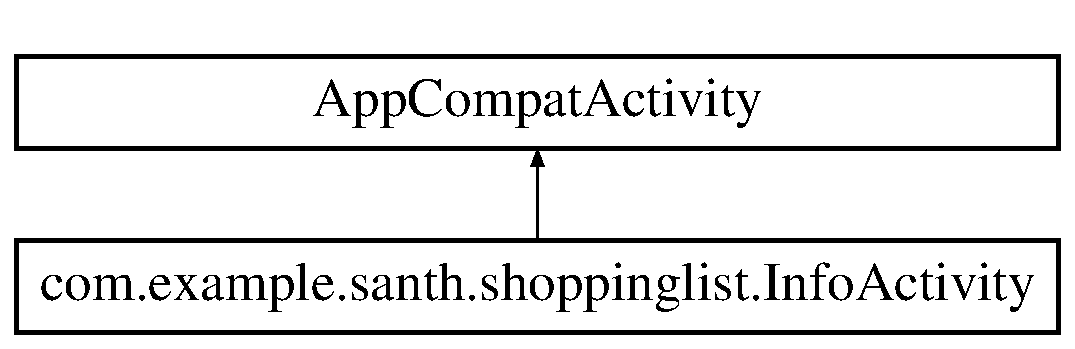
\includegraphics[height=2.000000cm]{classcom_1_1example_1_1santh_1_1shoppinglist_1_1_info_activity}
\end{center}
\end{figure}
\subsection*{Public Member Functions}
\begin{DoxyCompactItemize}
\item 
void \hyperlink{classcom_1_1example_1_1santh_1_1shoppinglist_1_1_info_activity_a17c7856d77bef5e3dc6ac5b71277e7be}{on\+Start} ()
\item 
void \hyperlink{classcom_1_1example_1_1santh_1_1shoppinglist_1_1_info_activity_a42122c7e17c3ba2e5676caed33110458}{on\+Stop} ()
\item 
boolean \hyperlink{classcom_1_1example_1_1santh_1_1shoppinglist_1_1_info_activity_a9e90836addabcf2d0ecd618cd5d425d2}{on\+Options\+Item\+Selected} (Menu\+Item item)
\begin{DoxyCompactList}\small\item\em on\+Options\+Item\+Selected to goback to \hyperlink{classcom_1_1example_1_1santh_1_1shoppinglist_1_1_main_activity}{Main\+Activity} \end{DoxyCompactList}\item 
void \hyperlink{classcom_1_1example_1_1santh_1_1shoppinglist_1_1_info_activity_ace2ec207701b823bdbf9af037cddcfdc}{on\+Back\+Pressed} ()
\begin{DoxyCompactList}\small\item\em on\+Back\+Pressed redirect to respective activity using intent \end{DoxyCompactList}\end{DoxyCompactItemize}
\subsection*{Static Public Attributes}
\begin{DoxyCompactItemize}
\item 
static final String \hyperlink{classcom_1_1example_1_1santh_1_1shoppinglist_1_1_info_activity_afe9ca10f6ddfc92fa9d03b57077341aa}{E\+X\+T\+R\+A\+\_\+\+M\+E\+S\+S\+A\+GE} = \char`\"{}com.\+example.\+santh.\+M\+E\+S\+S\+A\+GE\char`\"{}
\end{DoxyCompactItemize}
\subsection*{Protected Member Functions}
\begin{DoxyCompactItemize}
\item 
void \hyperlink{classcom_1_1example_1_1santh_1_1shoppinglist_1_1_info_activity_a7d41fdb42e01c39daa5d5036f2d26eba}{on\+Create} (Bundle saved\+Instance\+State)
\begin{DoxyCompactList}\small\item\em oncreate Method for Info Activity where titles and values are mapped \end{DoxyCompactList}\end{DoxyCompactItemize}


\subsection{Detailed Description}
Info Activity Class for description of App. 

\subsection{Member Function Documentation}
\index{com\+::example\+::santh\+::shoppinglist\+::\+Info\+Activity@{com\+::example\+::santh\+::shoppinglist\+::\+Info\+Activity}!on\+Back\+Pressed@{on\+Back\+Pressed}}
\index{on\+Back\+Pressed@{on\+Back\+Pressed}!com\+::example\+::santh\+::shoppinglist\+::\+Info\+Activity@{com\+::example\+::santh\+::shoppinglist\+::\+Info\+Activity}}
\subsubsection[{\texorpdfstring{on\+Back\+Pressed()}{onBackPressed()}}]{\setlength{\rightskip}{0pt plus 5cm}void com.\+example.\+santh.\+shoppinglist.\+Info\+Activity.\+on\+Back\+Pressed (
\begin{DoxyParamCaption}
{}
\end{DoxyParamCaption}
)}\hypertarget{classcom_1_1example_1_1santh_1_1shoppinglist_1_1_info_activity_ace2ec207701b823bdbf9af037cddcfdc}{}\label{classcom_1_1example_1_1santh_1_1shoppinglist_1_1_info_activity_ace2ec207701b823bdbf9af037cddcfdc}


on\+Back\+Pressed redirect to respective activity using intent 

\index{com\+::example\+::santh\+::shoppinglist\+::\+Info\+Activity@{com\+::example\+::santh\+::shoppinglist\+::\+Info\+Activity}!on\+Create@{on\+Create}}
\index{on\+Create@{on\+Create}!com\+::example\+::santh\+::shoppinglist\+::\+Info\+Activity@{com\+::example\+::santh\+::shoppinglist\+::\+Info\+Activity}}
\subsubsection[{\texorpdfstring{on\+Create(\+Bundle saved\+Instance\+State)}{onCreate(Bundle savedInstanceState)}}]{\setlength{\rightskip}{0pt plus 5cm}void com.\+example.\+santh.\+shoppinglist.\+Info\+Activity.\+on\+Create (
\begin{DoxyParamCaption}
\item[{Bundle}]{saved\+Instance\+State}
\end{DoxyParamCaption}
)\hspace{0.3cm}{\ttfamily [protected]}}\hypertarget{classcom_1_1example_1_1santh_1_1shoppinglist_1_1_info_activity_a7d41fdb42e01c39daa5d5036f2d26eba}{}\label{classcom_1_1example_1_1santh_1_1shoppinglist_1_1_info_activity_a7d41fdb42e01c39daa5d5036f2d26eba}


oncreate Method for Info Activity where titles and values are mapped 


\begin{DoxyParams}{Parameters}
{\em saved\+Instance\+State} & \\
\hline
\end{DoxyParams}
\index{com\+::example\+::santh\+::shoppinglist\+::\+Info\+Activity@{com\+::example\+::santh\+::shoppinglist\+::\+Info\+Activity}!on\+Options\+Item\+Selected@{on\+Options\+Item\+Selected}}
\index{on\+Options\+Item\+Selected@{on\+Options\+Item\+Selected}!com\+::example\+::santh\+::shoppinglist\+::\+Info\+Activity@{com\+::example\+::santh\+::shoppinglist\+::\+Info\+Activity}}
\subsubsection[{\texorpdfstring{on\+Options\+Item\+Selected(\+Menu\+Item item)}{onOptionsItemSelected(MenuItem item)}}]{\setlength{\rightskip}{0pt plus 5cm}boolean com.\+example.\+santh.\+shoppinglist.\+Info\+Activity.\+on\+Options\+Item\+Selected (
\begin{DoxyParamCaption}
\item[{Menu\+Item}]{item}
\end{DoxyParamCaption}
)}\hypertarget{classcom_1_1example_1_1santh_1_1shoppinglist_1_1_info_activity_a9e90836addabcf2d0ecd618cd5d425d2}{}\label{classcom_1_1example_1_1santh_1_1shoppinglist_1_1_info_activity_a9e90836addabcf2d0ecd618cd5d425d2}


on\+Options\+Item\+Selected to goback to \hyperlink{classcom_1_1example_1_1santh_1_1shoppinglist_1_1_main_activity}{Main\+Activity} 


\begin{DoxyParams}{Parameters}
{\em item} & \\
\hline
\end{DoxyParams}
\begin{DoxyReturn}{Returns}

\end{DoxyReturn}
\index{com\+::example\+::santh\+::shoppinglist\+::\+Info\+Activity@{com\+::example\+::santh\+::shoppinglist\+::\+Info\+Activity}!on\+Start@{on\+Start}}
\index{on\+Start@{on\+Start}!com\+::example\+::santh\+::shoppinglist\+::\+Info\+Activity@{com\+::example\+::santh\+::shoppinglist\+::\+Info\+Activity}}
\subsubsection[{\texorpdfstring{on\+Start()}{onStart()}}]{\setlength{\rightskip}{0pt plus 5cm}void com.\+example.\+santh.\+shoppinglist.\+Info\+Activity.\+on\+Start (
\begin{DoxyParamCaption}
{}
\end{DoxyParamCaption}
)}\hypertarget{classcom_1_1example_1_1santh_1_1shoppinglist_1_1_info_activity_a17c7856d77bef5e3dc6ac5b71277e7be}{}\label{classcom_1_1example_1_1santh_1_1shoppinglist_1_1_info_activity_a17c7856d77bef5e3dc6ac5b71277e7be}
\index{com\+::example\+::santh\+::shoppinglist\+::\+Info\+Activity@{com\+::example\+::santh\+::shoppinglist\+::\+Info\+Activity}!on\+Stop@{on\+Stop}}
\index{on\+Stop@{on\+Stop}!com\+::example\+::santh\+::shoppinglist\+::\+Info\+Activity@{com\+::example\+::santh\+::shoppinglist\+::\+Info\+Activity}}
\subsubsection[{\texorpdfstring{on\+Stop()}{onStop()}}]{\setlength{\rightskip}{0pt plus 5cm}void com.\+example.\+santh.\+shoppinglist.\+Info\+Activity.\+on\+Stop (
\begin{DoxyParamCaption}
{}
\end{DoxyParamCaption}
)}\hypertarget{classcom_1_1example_1_1santh_1_1shoppinglist_1_1_info_activity_a42122c7e17c3ba2e5676caed33110458}{}\label{classcom_1_1example_1_1santh_1_1shoppinglist_1_1_info_activity_a42122c7e17c3ba2e5676caed33110458}


\subsection{Member Data Documentation}
\index{com\+::example\+::santh\+::shoppinglist\+::\+Info\+Activity@{com\+::example\+::santh\+::shoppinglist\+::\+Info\+Activity}!E\+X\+T\+R\+A\+\_\+\+M\+E\+S\+S\+A\+GE@{E\+X\+T\+R\+A\+\_\+\+M\+E\+S\+S\+A\+GE}}
\index{E\+X\+T\+R\+A\+\_\+\+M\+E\+S\+S\+A\+GE@{E\+X\+T\+R\+A\+\_\+\+M\+E\+S\+S\+A\+GE}!com\+::example\+::santh\+::shoppinglist\+::\+Info\+Activity@{com\+::example\+::santh\+::shoppinglist\+::\+Info\+Activity}}
\subsubsection[{\texorpdfstring{E\+X\+T\+R\+A\+\_\+\+M\+E\+S\+S\+A\+GE}{EXTRA_MESSAGE}}]{\setlength{\rightskip}{0pt plus 5cm}final String com.\+example.\+santh.\+shoppinglist.\+Info\+Activity.\+E\+X\+T\+R\+A\+\_\+\+M\+E\+S\+S\+A\+GE = \char`\"{}com.\+example.\+santh.\+M\+E\+S\+S\+A\+GE\char`\"{}\hspace{0.3cm}{\ttfamily [static]}}\hypertarget{classcom_1_1example_1_1santh_1_1shoppinglist_1_1_info_activity_afe9ca10f6ddfc92fa9d03b57077341aa}{}\label{classcom_1_1example_1_1santh_1_1shoppinglist_1_1_info_activity_afe9ca10f6ddfc92fa9d03b57077341aa}


The documentation for this class was generated from the following file\+:\begin{DoxyCompactItemize}
\item 
E\+:/\+Android/\+Shopping\+List\+D\+B4 2/app/src/main/java/com/example/santh/shoppinglist/\hyperlink{_info_activity_8java}{Info\+Activity.\+java}\end{DoxyCompactItemize}

\hypertarget{classcom_1_1example_1_1santh_1_1shoppinglist_1_1_item_activity}{}\section{com.\+example.\+santh.\+shoppinglist.\+Item\+Activity Class Reference}
\label{classcom_1_1example_1_1santh_1_1shoppinglist_1_1_item_activity}\index{com.\+example.\+santh.\+shoppinglist.\+Item\+Activity@{com.\+example.\+santh.\+shoppinglist.\+Item\+Activity}}


This is a Item class which is used to add an item to list .Update the item.  


Inheritance diagram for com.\+example.\+santh.\+shoppinglist.\+Item\+Activity\+:\begin{figure}[H]
\begin{center}
\leavevmode
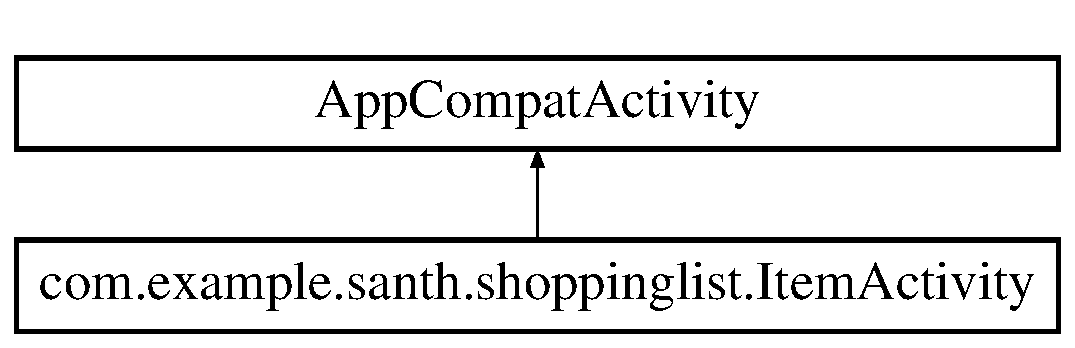
\includegraphics[height=2.000000cm]{classcom_1_1example_1_1santh_1_1shoppinglist_1_1_item_activity}
\end{center}
\end{figure}
\subsection*{Classes}
\begin{DoxyCompactItemize}
\item 
class {\bfseries Roll}
\end{DoxyCompactItemize}
\subsection*{Public Member Functions}
\begin{DoxyCompactItemize}
\item 
String\mbox{[}$\,$\mbox{]} \hyperlink{classcom_1_1example_1_1santh_1_1shoppinglist_1_1_item_activity_a2c84901261a54f907d418cc62a62bf01}{get\+Items\+From\+Db} (String search\+Term)
\item 
void \hyperlink{classcom_1_1example_1_1santh_1_1shoppinglist_1_1_item_activity_a3cee4a907695af2f1349dd36463fa232}{Add\+Item} (View view)
\begin{DoxyCompactList}\small\item\em this method adds an item to the List \end{DoxyCompactList}\item 
void \hyperlink{classcom_1_1example_1_1santh_1_1shoppinglist_1_1_item_activity_a2b50ca8d89997a96ca42966519e325d0}{Update\+Item} (View view)
\begin{DoxyCompactList}\small\item\em This method Updates Item in the List. \end{DoxyCompactList}\item 
boolean \hyperlink{classcom_1_1example_1_1santh_1_1shoppinglist_1_1_item_activity_a2292028973c391e424fe968564549bbb}{on\+Options\+Item\+Selected} (Menu\+Item item)
\begin{DoxyCompactList}\small\item\em Performs necessary action on clikcing respective menu item. \end{DoxyCompactList}\item 
void \hyperlink{classcom_1_1example_1_1santh_1_1shoppinglist_1_1_item_activity_afd0ec89a58aa62aead1e8532744900ba}{on\+Back\+Pressed} ()
\begin{DoxyCompactList}\small\item\em on\+Back\+Presses redirects to respective intent \end{DoxyCompactList}\item 
void \hyperlink{classcom_1_1example_1_1santh_1_1shoppinglist_1_1_item_activity_ad61e8de7cb10c59b8538c31a55370cd2}{goback} (View v)
\item 
boolean \hyperlink{classcom_1_1example_1_1santh_1_1shoppinglist_1_1_item_activity_aee5792c1c8583b7d0555ad2d2662f29a}{on\+Create\+Options\+Menu} (Menu menu)
\item 
void \hyperlink{classcom_1_1example_1_1santh_1_1shoppinglist_1_1_item_activity_a3073b08b8b6d85cf61e07d6087a06371}{on\+Voice} (View v)
\begin{DoxyCompactList}\small\item\em on\+Voice Method for Google Sppech to text C\+Onvertor \end{DoxyCompactList}\item 
void \hyperlink{classcom_1_1example_1_1santh_1_1shoppinglist_1_1_item_activity_a119c287029dd0cf1efb39e8d65a717b7}{on\+Cow} (View view)
\end{DoxyCompactItemize}
\subsection*{Protected Member Functions}
\begin{DoxyCompactItemize}
\item 
void \hyperlink{classcom_1_1example_1_1santh_1_1shoppinglist_1_1_item_activity_a9f23bfc5355a38c404138c7e2447c5ee}{on\+Create} (Bundle saved\+Instance\+State)
\begin{DoxyCompactList}\small\item\em oncreate method for setting up events of listview \end{DoxyCompactList}\item 
void \hyperlink{classcom_1_1example_1_1santh_1_1shoppinglist_1_1_item_activity_abc6d112c1fe2a4963352d90f9660e61b}{on\+Pause} ()
\item 
void \hyperlink{classcom_1_1example_1_1santh_1_1shoppinglist_1_1_item_activity_af86ebc29ccb94493c7dabb4c516fd722}{on\+Destroy} ()
\item 
void \hyperlink{classcom_1_1example_1_1santh_1_1shoppinglist_1_1_item_activity_ab91c203e6db796ab67bbf3101f17b184}{on\+Resume} ()
\item 
void \hyperlink{classcom_1_1example_1_1santh_1_1shoppinglist_1_1_item_activity_a8a4a685a91426c5780e1260d7348e486}{on\+Activity\+Result} (int request\+Code, int result\+Code, Intent data)
\begin{DoxyCompactList}\small\item\em on\+Activity\+Result method to retrieve Item\+Name from Google voice. \end{DoxyCompactList}\end{DoxyCompactItemize}
\subsection*{Static Protected Attributes}
\begin{DoxyCompactItemize}
\item 
static final int \hyperlink{classcom_1_1example_1_1santh_1_1shoppinglist_1_1_item_activity_aea6bca838db9041a53ce0cdc68c0410b}{R\+E\+S\+U\+L\+T\+\_\+\+S\+P\+E\+E\+CH} = 1
\end{DoxyCompactItemize}


\subsection{Detailed Description}
This is a Item class which is used to add an item to list .Update the item. 

It defines the List view on click listener and Long click Listener to perform edit and delete respectively 

\subsection{Member Function Documentation}
\index{com\+::example\+::santh\+::shoppinglist\+::\+Item\+Activity@{com\+::example\+::santh\+::shoppinglist\+::\+Item\+Activity}!Add\+Item@{Add\+Item}}
\index{Add\+Item@{Add\+Item}!com\+::example\+::santh\+::shoppinglist\+::\+Item\+Activity@{com\+::example\+::santh\+::shoppinglist\+::\+Item\+Activity}}
\subsubsection[{\texorpdfstring{Add\+Item(\+View view)}{AddItem(View view)}}]{\setlength{\rightskip}{0pt plus 5cm}void com.\+example.\+santh.\+shoppinglist.\+Item\+Activity.\+Add\+Item (
\begin{DoxyParamCaption}
\item[{View}]{view}
\end{DoxyParamCaption}
)}\hypertarget{classcom_1_1example_1_1santh_1_1shoppinglist_1_1_item_activity_a3cee4a907695af2f1349dd36463fa232}{}\label{classcom_1_1example_1_1santh_1_1shoppinglist_1_1_item_activity_a3cee4a907695af2f1349dd36463fa232}


this method adds an item to the List 


\begin{DoxyParams}{Parameters}
{\em view} & \\
\hline
\end{DoxyParams}
\index{com\+::example\+::santh\+::shoppinglist\+::\+Item\+Activity@{com\+::example\+::santh\+::shoppinglist\+::\+Item\+Activity}!get\+Items\+From\+Db@{get\+Items\+From\+Db}}
\index{get\+Items\+From\+Db@{get\+Items\+From\+Db}!com\+::example\+::santh\+::shoppinglist\+::\+Item\+Activity@{com\+::example\+::santh\+::shoppinglist\+::\+Item\+Activity}}
\subsubsection[{\texorpdfstring{get\+Items\+From\+Db(\+String search\+Term)}{getItemsFromDb(String searchTerm)}}]{\setlength{\rightskip}{0pt plus 5cm}String \mbox{[}$\,$\mbox{]} com.\+example.\+santh.\+shoppinglist.\+Item\+Activity.\+get\+Items\+From\+Db (
\begin{DoxyParamCaption}
\item[{String}]{search\+Term}
\end{DoxyParamCaption}
)}\hypertarget{classcom_1_1example_1_1santh_1_1shoppinglist_1_1_item_activity_a2c84901261a54f907d418cc62a62bf01}{}\label{classcom_1_1example_1_1santh_1_1shoppinglist_1_1_item_activity_a2c84901261a54f907d418cc62a62bf01}
\index{com\+::example\+::santh\+::shoppinglist\+::\+Item\+Activity@{com\+::example\+::santh\+::shoppinglist\+::\+Item\+Activity}!goback@{goback}}
\index{goback@{goback}!com\+::example\+::santh\+::shoppinglist\+::\+Item\+Activity@{com\+::example\+::santh\+::shoppinglist\+::\+Item\+Activity}}
\subsubsection[{\texorpdfstring{goback(\+View v)}{goback(View v)}}]{\setlength{\rightskip}{0pt plus 5cm}void com.\+example.\+santh.\+shoppinglist.\+Item\+Activity.\+goback (
\begin{DoxyParamCaption}
\item[{View}]{v}
\end{DoxyParamCaption}
)}\hypertarget{classcom_1_1example_1_1santh_1_1shoppinglist_1_1_item_activity_ad61e8de7cb10c59b8538c31a55370cd2}{}\label{classcom_1_1example_1_1santh_1_1shoppinglist_1_1_item_activity_ad61e8de7cb10c59b8538c31a55370cd2}
\index{com\+::example\+::santh\+::shoppinglist\+::\+Item\+Activity@{com\+::example\+::santh\+::shoppinglist\+::\+Item\+Activity}!on\+Activity\+Result@{on\+Activity\+Result}}
\index{on\+Activity\+Result@{on\+Activity\+Result}!com\+::example\+::santh\+::shoppinglist\+::\+Item\+Activity@{com\+::example\+::santh\+::shoppinglist\+::\+Item\+Activity}}
\subsubsection[{\texorpdfstring{on\+Activity\+Result(int request\+Code, int result\+Code, Intent data)}{onActivityResult(int requestCode, int resultCode, Intent data)}}]{\setlength{\rightskip}{0pt plus 5cm}void com.\+example.\+santh.\+shoppinglist.\+Item\+Activity.\+on\+Activity\+Result (
\begin{DoxyParamCaption}
\item[{int}]{request\+Code, }
\item[{int}]{result\+Code, }
\item[{Intent}]{data}
\end{DoxyParamCaption}
)\hspace{0.3cm}{\ttfamily [protected]}}\hypertarget{classcom_1_1example_1_1santh_1_1shoppinglist_1_1_item_activity_a8a4a685a91426c5780e1260d7348e486}{}\label{classcom_1_1example_1_1santh_1_1shoppinglist_1_1_item_activity_a8a4a685a91426c5780e1260d7348e486}


on\+Activity\+Result method to retrieve Item\+Name from Google voice. 


\begin{DoxyParams}{Parameters}
{\em request\+Code} & \\
\hline
{\em result\+Code} & \\
\hline
{\em data} & \\
\hline
\end{DoxyParams}
\index{com\+::example\+::santh\+::shoppinglist\+::\+Item\+Activity@{com\+::example\+::santh\+::shoppinglist\+::\+Item\+Activity}!on\+Back\+Pressed@{on\+Back\+Pressed}}
\index{on\+Back\+Pressed@{on\+Back\+Pressed}!com\+::example\+::santh\+::shoppinglist\+::\+Item\+Activity@{com\+::example\+::santh\+::shoppinglist\+::\+Item\+Activity}}
\subsubsection[{\texorpdfstring{on\+Back\+Pressed()}{onBackPressed()}}]{\setlength{\rightskip}{0pt plus 5cm}void com.\+example.\+santh.\+shoppinglist.\+Item\+Activity.\+on\+Back\+Pressed (
\begin{DoxyParamCaption}
{}
\end{DoxyParamCaption}
)}\hypertarget{classcom_1_1example_1_1santh_1_1shoppinglist_1_1_item_activity_afd0ec89a58aa62aead1e8532744900ba}{}\label{classcom_1_1example_1_1santh_1_1shoppinglist_1_1_item_activity_afd0ec89a58aa62aead1e8532744900ba}


on\+Back\+Presses redirects to respective intent 

\index{com\+::example\+::santh\+::shoppinglist\+::\+Item\+Activity@{com\+::example\+::santh\+::shoppinglist\+::\+Item\+Activity}!on\+Cow@{on\+Cow}}
\index{on\+Cow@{on\+Cow}!com\+::example\+::santh\+::shoppinglist\+::\+Item\+Activity@{com\+::example\+::santh\+::shoppinglist\+::\+Item\+Activity}}
\subsubsection[{\texorpdfstring{on\+Cow(\+View view)}{onCow(View view)}}]{\setlength{\rightskip}{0pt plus 5cm}void com.\+example.\+santh.\+shoppinglist.\+Item\+Activity.\+on\+Cow (
\begin{DoxyParamCaption}
\item[{View}]{view}
\end{DoxyParamCaption}
)}\hypertarget{classcom_1_1example_1_1santh_1_1shoppinglist_1_1_item_activity_a119c287029dd0cf1efb39e8d65a717b7}{}\label{classcom_1_1example_1_1santh_1_1shoppinglist_1_1_item_activity_a119c287029dd0cf1efb39e8d65a717b7}
\index{com\+::example\+::santh\+::shoppinglist\+::\+Item\+Activity@{com\+::example\+::santh\+::shoppinglist\+::\+Item\+Activity}!on\+Create@{on\+Create}}
\index{on\+Create@{on\+Create}!com\+::example\+::santh\+::shoppinglist\+::\+Item\+Activity@{com\+::example\+::santh\+::shoppinglist\+::\+Item\+Activity}}
\subsubsection[{\texorpdfstring{on\+Create(\+Bundle saved\+Instance\+State)}{onCreate(Bundle savedInstanceState)}}]{\setlength{\rightskip}{0pt plus 5cm}void com.\+example.\+santh.\+shoppinglist.\+Item\+Activity.\+on\+Create (
\begin{DoxyParamCaption}
\item[{Bundle}]{saved\+Instance\+State}
\end{DoxyParamCaption}
)\hspace{0.3cm}{\ttfamily [protected]}}\hypertarget{classcom_1_1example_1_1santh_1_1shoppinglist_1_1_item_activity_a9f23bfc5355a38c404138c7e2447c5ee}{}\label{classcom_1_1example_1_1santh_1_1shoppinglist_1_1_item_activity_a9f23bfc5355a38c404138c7e2447c5ee}


oncreate method for setting up events of listview 


\begin{DoxyParams}{Parameters}
{\em saved\+Instance\+State} & \\
\hline
\end{DoxyParams}
\index{com\+::example\+::santh\+::shoppinglist\+::\+Item\+Activity@{com\+::example\+::santh\+::shoppinglist\+::\+Item\+Activity}!on\+Create\+Options\+Menu@{on\+Create\+Options\+Menu}}
\index{on\+Create\+Options\+Menu@{on\+Create\+Options\+Menu}!com\+::example\+::santh\+::shoppinglist\+::\+Item\+Activity@{com\+::example\+::santh\+::shoppinglist\+::\+Item\+Activity}}
\subsubsection[{\texorpdfstring{on\+Create\+Options\+Menu(\+Menu menu)}{onCreateOptionsMenu(Menu menu)}}]{\setlength{\rightskip}{0pt plus 5cm}boolean com.\+example.\+santh.\+shoppinglist.\+Item\+Activity.\+on\+Create\+Options\+Menu (
\begin{DoxyParamCaption}
\item[{Menu}]{menu}
\end{DoxyParamCaption}
)}\hypertarget{classcom_1_1example_1_1santh_1_1shoppinglist_1_1_item_activity_aee5792c1c8583b7d0555ad2d2662f29a}{}\label{classcom_1_1example_1_1santh_1_1shoppinglist_1_1_item_activity_aee5792c1c8583b7d0555ad2d2662f29a}
\index{com\+::example\+::santh\+::shoppinglist\+::\+Item\+Activity@{com\+::example\+::santh\+::shoppinglist\+::\+Item\+Activity}!on\+Destroy@{on\+Destroy}}
\index{on\+Destroy@{on\+Destroy}!com\+::example\+::santh\+::shoppinglist\+::\+Item\+Activity@{com\+::example\+::santh\+::shoppinglist\+::\+Item\+Activity}}
\subsubsection[{\texorpdfstring{on\+Destroy()}{onDestroy()}}]{\setlength{\rightskip}{0pt plus 5cm}void com.\+example.\+santh.\+shoppinglist.\+Item\+Activity.\+on\+Destroy (
\begin{DoxyParamCaption}
{}
\end{DoxyParamCaption}
)\hspace{0.3cm}{\ttfamily [protected]}}\hypertarget{classcom_1_1example_1_1santh_1_1shoppinglist_1_1_item_activity_af86ebc29ccb94493c7dabb4c516fd722}{}\label{classcom_1_1example_1_1santh_1_1shoppinglist_1_1_item_activity_af86ebc29ccb94493c7dabb4c516fd722}
\index{com\+::example\+::santh\+::shoppinglist\+::\+Item\+Activity@{com\+::example\+::santh\+::shoppinglist\+::\+Item\+Activity}!on\+Options\+Item\+Selected@{on\+Options\+Item\+Selected}}
\index{on\+Options\+Item\+Selected@{on\+Options\+Item\+Selected}!com\+::example\+::santh\+::shoppinglist\+::\+Item\+Activity@{com\+::example\+::santh\+::shoppinglist\+::\+Item\+Activity}}
\subsubsection[{\texorpdfstring{on\+Options\+Item\+Selected(\+Menu\+Item item)}{onOptionsItemSelected(MenuItem item)}}]{\setlength{\rightskip}{0pt plus 5cm}boolean com.\+example.\+santh.\+shoppinglist.\+Item\+Activity.\+on\+Options\+Item\+Selected (
\begin{DoxyParamCaption}
\item[{Menu\+Item}]{item}
\end{DoxyParamCaption}
)}\hypertarget{classcom_1_1example_1_1santh_1_1shoppinglist_1_1_item_activity_a2292028973c391e424fe968564549bbb}{}\label{classcom_1_1example_1_1santh_1_1shoppinglist_1_1_item_activity_a2292028973c391e424fe968564549bbb}


Performs necessary action on clikcing respective menu item. 


\begin{DoxyParams}{Parameters}
{\em item} & \\
\hline
\end{DoxyParams}
\begin{DoxyReturn}{Returns}

\end{DoxyReturn}
\index{com\+::example\+::santh\+::shoppinglist\+::\+Item\+Activity@{com\+::example\+::santh\+::shoppinglist\+::\+Item\+Activity}!on\+Pause@{on\+Pause}}
\index{on\+Pause@{on\+Pause}!com\+::example\+::santh\+::shoppinglist\+::\+Item\+Activity@{com\+::example\+::santh\+::shoppinglist\+::\+Item\+Activity}}
\subsubsection[{\texorpdfstring{on\+Pause()}{onPause()}}]{\setlength{\rightskip}{0pt plus 5cm}void com.\+example.\+santh.\+shoppinglist.\+Item\+Activity.\+on\+Pause (
\begin{DoxyParamCaption}
{}
\end{DoxyParamCaption}
)\hspace{0.3cm}{\ttfamily [protected]}}\hypertarget{classcom_1_1example_1_1santh_1_1shoppinglist_1_1_item_activity_abc6d112c1fe2a4963352d90f9660e61b}{}\label{classcom_1_1example_1_1santh_1_1shoppinglist_1_1_item_activity_abc6d112c1fe2a4963352d90f9660e61b}
\index{com\+::example\+::santh\+::shoppinglist\+::\+Item\+Activity@{com\+::example\+::santh\+::shoppinglist\+::\+Item\+Activity}!on\+Resume@{on\+Resume}}
\index{on\+Resume@{on\+Resume}!com\+::example\+::santh\+::shoppinglist\+::\+Item\+Activity@{com\+::example\+::santh\+::shoppinglist\+::\+Item\+Activity}}
\subsubsection[{\texorpdfstring{on\+Resume()}{onResume()}}]{\setlength{\rightskip}{0pt plus 5cm}void com.\+example.\+santh.\+shoppinglist.\+Item\+Activity.\+on\+Resume (
\begin{DoxyParamCaption}
{}
\end{DoxyParamCaption}
)\hspace{0.3cm}{\ttfamily [protected]}}\hypertarget{classcom_1_1example_1_1santh_1_1shoppinglist_1_1_item_activity_ab91c203e6db796ab67bbf3101f17b184}{}\label{classcom_1_1example_1_1santh_1_1shoppinglist_1_1_item_activity_ab91c203e6db796ab67bbf3101f17b184}
\index{com\+::example\+::santh\+::shoppinglist\+::\+Item\+Activity@{com\+::example\+::santh\+::shoppinglist\+::\+Item\+Activity}!on\+Voice@{on\+Voice}}
\index{on\+Voice@{on\+Voice}!com\+::example\+::santh\+::shoppinglist\+::\+Item\+Activity@{com\+::example\+::santh\+::shoppinglist\+::\+Item\+Activity}}
\subsubsection[{\texorpdfstring{on\+Voice(\+View v)}{onVoice(View v)}}]{\setlength{\rightskip}{0pt plus 5cm}void com.\+example.\+santh.\+shoppinglist.\+Item\+Activity.\+on\+Voice (
\begin{DoxyParamCaption}
\item[{View}]{v}
\end{DoxyParamCaption}
)}\hypertarget{classcom_1_1example_1_1santh_1_1shoppinglist_1_1_item_activity_a3073b08b8b6d85cf61e07d6087a06371}{}\label{classcom_1_1example_1_1santh_1_1shoppinglist_1_1_item_activity_a3073b08b8b6d85cf61e07d6087a06371}


on\+Voice Method for Google Sppech to text C\+Onvertor 


\begin{DoxyParams}{Parameters}
{\em v} & \\
\hline
\end{DoxyParams}
\index{com\+::example\+::santh\+::shoppinglist\+::\+Item\+Activity@{com\+::example\+::santh\+::shoppinglist\+::\+Item\+Activity}!Update\+Item@{Update\+Item}}
\index{Update\+Item@{Update\+Item}!com\+::example\+::santh\+::shoppinglist\+::\+Item\+Activity@{com\+::example\+::santh\+::shoppinglist\+::\+Item\+Activity}}
\subsubsection[{\texorpdfstring{Update\+Item(\+View view)}{UpdateItem(View view)}}]{\setlength{\rightskip}{0pt plus 5cm}void com.\+example.\+santh.\+shoppinglist.\+Item\+Activity.\+Update\+Item (
\begin{DoxyParamCaption}
\item[{View}]{view}
\end{DoxyParamCaption}
)}\hypertarget{classcom_1_1example_1_1santh_1_1shoppinglist_1_1_item_activity_a2b50ca8d89997a96ca42966519e325d0}{}\label{classcom_1_1example_1_1santh_1_1shoppinglist_1_1_item_activity_a2b50ca8d89997a96ca42966519e325d0}


This method Updates Item in the List. 


\begin{DoxyParams}{Parameters}
{\em view} & \\
\hline
\end{DoxyParams}


\subsection{Member Data Documentation}
\index{com\+::example\+::santh\+::shoppinglist\+::\+Item\+Activity@{com\+::example\+::santh\+::shoppinglist\+::\+Item\+Activity}!R\+E\+S\+U\+L\+T\+\_\+\+S\+P\+E\+E\+CH@{R\+E\+S\+U\+L\+T\+\_\+\+S\+P\+E\+E\+CH}}
\index{R\+E\+S\+U\+L\+T\+\_\+\+S\+P\+E\+E\+CH@{R\+E\+S\+U\+L\+T\+\_\+\+S\+P\+E\+E\+CH}!com\+::example\+::santh\+::shoppinglist\+::\+Item\+Activity@{com\+::example\+::santh\+::shoppinglist\+::\+Item\+Activity}}
\subsubsection[{\texorpdfstring{R\+E\+S\+U\+L\+T\+\_\+\+S\+P\+E\+E\+CH}{RESULT_SPEECH}}]{\setlength{\rightskip}{0pt plus 5cm}final int com.\+example.\+santh.\+shoppinglist.\+Item\+Activity.\+R\+E\+S\+U\+L\+T\+\_\+\+S\+P\+E\+E\+CH = 1\hspace{0.3cm}{\ttfamily [static]}, {\ttfamily [protected]}}\hypertarget{classcom_1_1example_1_1santh_1_1shoppinglist_1_1_item_activity_aea6bca838db9041a53ce0cdc68c0410b}{}\label{classcom_1_1example_1_1santh_1_1shoppinglist_1_1_item_activity_aea6bca838db9041a53ce0cdc68c0410b}


The documentation for this class was generated from the following file\+:\begin{DoxyCompactItemize}
\item 
E\+:/\+Android/\+Shopping\+List\+D\+B4 2/app/src/main/java/com/example/santh/shoppinglist/\hyperlink{_item_activity_8java}{Item\+Activity.\+java}\end{DoxyCompactItemize}

\hypertarget{classcom_1_1example_1_1santh_1_1shoppinglist_1_1_j_s_o_n_parser}{}\section{com.\+example.\+santh.\+shoppinglist.\+J\+S\+O\+N\+Parser Class Reference}
\label{classcom_1_1example_1_1santh_1_1shoppinglist_1_1_j_s_o_n_parser}\index{com.\+example.\+santh.\+shoppinglist.\+J\+S\+O\+N\+Parser@{com.\+example.\+santh.\+shoppinglist.\+J\+S\+O\+N\+Parser}}


J\+S\+ON Parser class to convert entries into J\+S\+ON array.  


\subsection*{Public Member Functions}
\begin{DoxyCompactItemize}
\item 
J\+S\+O\+N\+Object \hyperlink{classcom_1_1example_1_1santh_1_1shoppinglist_1_1_j_s_o_n_parser_a1fb3f6c658814c1373623ecdf65cb103}{make\+Http\+Request} (String url, String method, Hash\+Map$<$ String, String $>$ params)
\end{DoxyCompactItemize}


\subsection{Detailed Description}
J\+S\+ON Parser class to convert entries into J\+S\+ON array. 

\subsection{Member Function Documentation}
\index{com\+::example\+::santh\+::shoppinglist\+::\+J\+S\+O\+N\+Parser@{com\+::example\+::santh\+::shoppinglist\+::\+J\+S\+O\+N\+Parser}!make\+Http\+Request@{make\+Http\+Request}}
\index{make\+Http\+Request@{make\+Http\+Request}!com\+::example\+::santh\+::shoppinglist\+::\+J\+S\+O\+N\+Parser@{com\+::example\+::santh\+::shoppinglist\+::\+J\+S\+O\+N\+Parser}}
\subsubsection[{\texorpdfstring{make\+Http\+Request(\+String url, String method, Hash\+Map$<$ String, String $>$ params)}{makeHttpRequest(String url, String method, HashMap< String, String > params)}}]{\setlength{\rightskip}{0pt plus 5cm}J\+S\+O\+N\+Object com.\+example.\+santh.\+shoppinglist.\+J\+S\+O\+N\+Parser.\+make\+Http\+Request (
\begin{DoxyParamCaption}
\item[{String}]{url, }
\item[{String}]{method, }
\item[{Hash\+Map$<$ String, String $>$}]{params}
\end{DoxyParamCaption}
)}\hypertarget{classcom_1_1example_1_1santh_1_1shoppinglist_1_1_j_s_o_n_parser_a1fb3f6c658814c1373623ecdf65cb103}{}\label{classcom_1_1example_1_1santh_1_1shoppinglist_1_1_j_s_o_n_parser_a1fb3f6c658814c1373623ecdf65cb103}


The documentation for this class was generated from the following file\+:\begin{DoxyCompactItemize}
\item 
E\+:/\+Android/\+Shopping\+List\+D\+B4 2/app/src/main/java/com/example/santh/shoppinglist/\hyperlink{_j_s_o_n_parser_8java}{J\+S\+O\+N\+Parser.\+java}\end{DoxyCompactItemize}

\hypertarget{classcom_1_1example_1_1santh_1_1shoppinglist_1_1_launch_activity}{}\section{com.\+example.\+santh.\+shoppinglist.\+Launch\+Activity Class Reference}
\label{classcom_1_1example_1_1santh_1_1shoppinglist_1_1_launch_activity}\index{com.\+example.\+santh.\+shoppinglist.\+Launch\+Activity@{com.\+example.\+santh.\+shoppinglist.\+Launch\+Activity}}


\hyperlink{classcom_1_1example_1_1santh_1_1shoppinglist_1_1_launch_activity}{Launch\+Activity} for Splash\+Screen and calling threads to link external hp scripts with internal database .  


Inheritance diagram for com.\+example.\+santh.\+shoppinglist.\+Launch\+Activity\+:\begin{figure}[H]
\begin{center}
\leavevmode
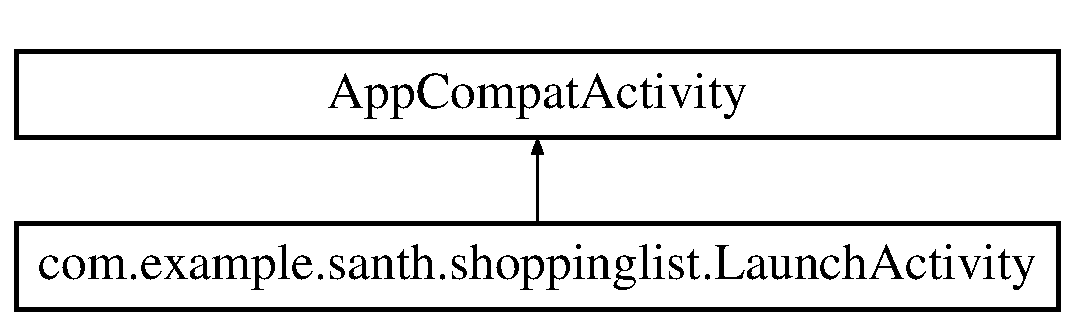
\includegraphics[height=2.000000cm]{classcom_1_1example_1_1santh_1_1shoppinglist_1_1_launch_activity}
\end{center}
\end{figure}
\subsection*{Public Member Functions}
\begin{DoxyCompactItemize}
\item 
boolean \hyperlink{classcom_1_1example_1_1santh_1_1shoppinglist_1_1_launch_activity_a2c64bd9594abeff8779f4c111479daf1}{is\+Online} ()
\begin{DoxyCompactList}\small\item\em Determines if the device is internet able. \end{DoxyCompactList}\end{DoxyCompactItemize}
\subsection*{Protected Member Functions}
\begin{DoxyCompactItemize}
\item 
void \hyperlink{classcom_1_1example_1_1santh_1_1shoppinglist_1_1_launch_activity_aecdd335077ec29041aa645bd6977c43d}{on\+Create} (Bundle saved\+Instance\+State)
\begin{DoxyCompactList}\small\item\em Called when the activity is first created. \end{DoxyCompactList}\end{DoxyCompactItemize}


\subsection{Detailed Description}
\hyperlink{classcom_1_1example_1_1santh_1_1shoppinglist_1_1_launch_activity}{Launch\+Activity} for Splash\+Screen and calling threads to link external hp scripts with internal database . 

\subsection{Member Function Documentation}
\index{com\+::example\+::santh\+::shoppinglist\+::\+Launch\+Activity@{com\+::example\+::santh\+::shoppinglist\+::\+Launch\+Activity}!is\+Online@{is\+Online}}
\index{is\+Online@{is\+Online}!com\+::example\+::santh\+::shoppinglist\+::\+Launch\+Activity@{com\+::example\+::santh\+::shoppinglist\+::\+Launch\+Activity}}
\subsubsection[{\texorpdfstring{is\+Online()}{isOnline()}}]{\setlength{\rightskip}{0pt plus 5cm}boolean com.\+example.\+santh.\+shoppinglist.\+Launch\+Activity.\+is\+Online (
\begin{DoxyParamCaption}
{}
\end{DoxyParamCaption}
)}\hypertarget{classcom_1_1example_1_1santh_1_1shoppinglist_1_1_launch_activity_a2c64bd9594abeff8779f4c111479daf1}{}\label{classcom_1_1example_1_1santh_1_1shoppinglist_1_1_launch_activity_a2c64bd9594abeff8779f4c111479daf1}


Determines if the device is internet able. 

\index{com\+::example\+::santh\+::shoppinglist\+::\+Launch\+Activity@{com\+::example\+::santh\+::shoppinglist\+::\+Launch\+Activity}!on\+Create@{on\+Create}}
\index{on\+Create@{on\+Create}!com\+::example\+::santh\+::shoppinglist\+::\+Launch\+Activity@{com\+::example\+::santh\+::shoppinglist\+::\+Launch\+Activity}}
\subsubsection[{\texorpdfstring{on\+Create(\+Bundle saved\+Instance\+State)}{onCreate(Bundle savedInstanceState)}}]{\setlength{\rightskip}{0pt plus 5cm}void com.\+example.\+santh.\+shoppinglist.\+Launch\+Activity.\+on\+Create (
\begin{DoxyParamCaption}
\item[{Bundle}]{saved\+Instance\+State}
\end{DoxyParamCaption}
)\hspace{0.3cm}{\ttfamily [protected]}}\hypertarget{classcom_1_1example_1_1santh_1_1shoppinglist_1_1_launch_activity_aecdd335077ec29041aa645bd6977c43d}{}\label{classcom_1_1example_1_1santh_1_1shoppinglist_1_1_launch_activity_aecdd335077ec29041aa645bd6977c43d}


Called when the activity is first created. 



The documentation for this class was generated from the following file\+:\begin{DoxyCompactItemize}
\item 
E\+:/\+Android/\+Shopping\+List\+D\+B4 2/app/src/main/java/com/example/santh/shoppinglist/\hyperlink{_launch_activity_8java}{Launch\+Activity.\+java}\end{DoxyCompactItemize}

\hypertarget{classcom_1_1example_1_1santh_1_1shoppinglist_1_1_list_activity}{}\section{com.\+example.\+santh.\+shoppinglist.\+List\+Activity Class Reference}
\label{classcom_1_1example_1_1santh_1_1shoppinglist_1_1_list_activity}\index{com.\+example.\+santh.\+shoppinglist.\+List\+Activity@{com.\+example.\+santh.\+shoppinglist.\+List\+Activity}}


List Activity Class is used to represent all items with their respective information and performs delete operation of item and cross over.  


Inheritance diagram for com.\+example.\+santh.\+shoppinglist.\+List\+Activity\+:\begin{figure}[H]
\begin{center}
\leavevmode
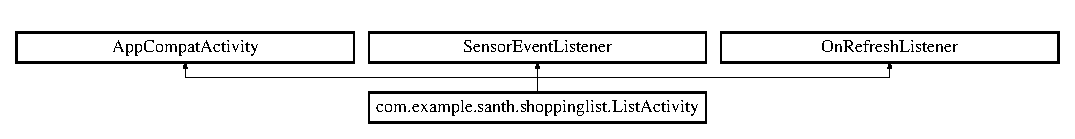
\includegraphics[height=1.424936cm]{classcom_1_1example_1_1santh_1_1shoppinglist_1_1_list_activity}
\end{center}
\end{figure}
\subsection*{Classes}
\begin{DoxyCompactItemize}
\item 
class {\bfseries New\+Sync\+Items}
\item 
class {\bfseries Syncexternal}
\end{DoxyCompactItemize}
\subsection*{Public Member Functions}
\begin{DoxyCompactItemize}
\item 
void \hyperlink{classcom_1_1example_1_1santh_1_1shoppinglist_1_1_list_activity_ad2d33376b6c33875d85c9250077c7f0a}{on\+Accuracy\+Changed} (Sensor sensor, int accuracy)
\item 
void \hyperlink{classcom_1_1example_1_1santh_1_1shoppinglist_1_1_list_activity_a3fe70255c4756fc99021e0ed27683548}{on\+Sensor\+Changed} (Sensor\+Event event)
\begin{DoxyCompactList}\small\item\em on detecting Shake Delete all Items in the List \end{DoxyCompactList}\item 
void \hyperlink{classcom_1_1example_1_1santh_1_1shoppinglist_1_1_list_activity_ab9ad7fc938dbd932094363fc1e56eac9}{on\+Sensor\+Change} (Sensor\+Event sensor\+Event)
\item 
boolean \hyperlink{classcom_1_1example_1_1santh_1_1shoppinglist_1_1_list_activity_a89a36a191d70c8b9d07db5eda2e804e4}{on\+Create\+Options\+Menu} (Menu menu)
\item 
void \hyperlink{classcom_1_1example_1_1santh_1_1shoppinglist_1_1_list_activity_a3aa761782d9eb5c28ec21734e407970d}{Add\+Item} (View v)
\begin{DoxyCompactList}\small\item\em Add Item rediretcs to Item activity. \end{DoxyCompactList}\item 
boolean \hyperlink{classcom_1_1example_1_1santh_1_1shoppinglist_1_1_list_activity_a1a93b6350edb03460299def603c57a44}{is\+Online} ()
\begin{DoxyCompactList}\small\item\em Determines if the device is internet able. \end{DoxyCompactList}\item 
void \hyperlink{classcom_1_1example_1_1santh_1_1shoppinglist_1_1_list_activity_a019462edc2e1d011fe110720b294fe41}{Sync\+Items} (View v)
\item 
void \hyperlink{classcom_1_1example_1_1santh_1_1shoppinglist_1_1_list_activity_aeb713dae9574328c1179a3a1fe298365}{on\+Refresh} ()
\item 
boolean \hyperlink{classcom_1_1example_1_1santh_1_1shoppinglist_1_1_list_activity_a07f94ec03899822148ce095082318cdb}{on\+Options\+Item\+Selected} (Menu\+Item item)
\begin{DoxyCompactList}\small\item\em Performs necessary function on clicking respective Menu Item. \end{DoxyCompactList}\item 
void \hyperlink{classcom_1_1example_1_1santh_1_1shoppinglist_1_1_list_activity_ac120c9e11a30ad182b0c2e146bbc420a}{Deletedialog} ()
\begin{DoxyCompactList}\small\item\em Delete all Items in the List. \end{DoxyCompactList}\item 
void \hyperlink{classcom_1_1example_1_1santh_1_1shoppinglist_1_1_list_activity_a3e5d96fe6cb761f9b036c552a5078406}{display\+Data\+Custom} ()
\begin{DoxyCompactList}\small\item\em Send Data to \hyperlink{classcom_1_1example_1_1santh_1_1shoppinglist_1_1_my_custom_adapter}{My\+Custom\+Adapter}. \end{DoxyCompactList}\item 
void \hyperlink{classcom_1_1example_1_1santh_1_1shoppinglist_1_1_list_activity_ae309a9528aeacc4614e63dd6946bbdfe}{get\+Price} ()
\begin{DoxyCompactList}\small\item\em Show the price of List. \end{DoxyCompactList}\item 
void \hyperlink{classcom_1_1example_1_1santh_1_1shoppinglist_1_1_list_activity_a5941058d8bb35fffa810cdc1bc7cb78b}{on\+Back\+Pressed} ()
\begin{DoxyCompactList}\small\item\em Back Pressed method. \end{DoxyCompactList}\end{DoxyCompactItemize}
\subsection*{Static Public Member Functions}
\begin{DoxyCompactItemize}
\item 
static final boolean \hyperlink{classcom_1_1example_1_1santh_1_1shoppinglist_1_1_list_activity_a67c3e8b285551793d2095968b583c92e}{is\+Valid\+Email} (Char\+Sequence target)
\end{DoxyCompactItemize}
\subsection*{Public Attributes}
\begin{DoxyCompactItemize}
\item 
Alert\+Dialog \hyperlink{classcom_1_1example_1_1santh_1_1shoppinglist_1_1_list_activity_a10f069d18425057cd9c3c13a3a1ab011}{my\+Alert\+Dialog}
\item 
Alert\+Dialog \hyperlink{classcom_1_1example_1_1santh_1_1shoppinglist_1_1_list_activity_ad19898c97695f5a48727227122c055dd}{my2\+Alert\+Dialog}
\end{DoxyCompactItemize}
\subsection*{Protected Member Functions}
\begin{DoxyCompactItemize}
\item 
void \hyperlink{classcom_1_1example_1_1santh_1_1shoppinglist_1_1_list_activity_affe7979f09447f88b742e0a27f2469a2}{on\+Create} (Bundle saved\+Instance\+State)
\begin{DoxyCompactList}\small\item\em on\+Create Method for setting up Listview Events \end{DoxyCompactList}\item 
void \hyperlink{classcom_1_1example_1_1santh_1_1shoppinglist_1_1_list_activity_a656f84d86a0cf1302ac1961f241fcefe}{on\+Pause} ()
\begin{DoxyCompactList}\small\item\em on\+Pause method to pause the sensor\+Manager \end{DoxyCompactList}\item 
void \hyperlink{classcom_1_1example_1_1santh_1_1shoppinglist_1_1_list_activity_a03da83dbc50946c4de153f3f8ccb20d5}{on\+Destroy} ()
\begin{DoxyCompactList}\small\item\em on\+Destroy Method . \end{DoxyCompactList}\item 
void \hyperlink{classcom_1_1example_1_1santh_1_1shoppinglist_1_1_list_activity_a7d54b1d68cbd82fb0468b4401e0730bd}{on\+Resume} ()
\begin{DoxyCompactList}\small\item\em on\+Resume Method for resuming the sensor \end{DoxyCompactList}\end{DoxyCompactItemize}
\subsection*{Static Protected Attributes}
\begin{DoxyCompactItemize}
\item 
static final int \hyperlink{classcom_1_1example_1_1santh_1_1shoppinglist_1_1_list_activity_ae837f52436477b84e95460db4cc00cec}{R\+E\+S\+U\+L\+T\+\_\+\+S\+P\+E\+E\+CH} = 1
\end{DoxyCompactItemize}


\subsection{Detailed Description}
List Activity Class is used to represent all items with their respective information and performs delete operation of item and cross over. 

It defines the List view on click listener and Long click Listener to perform edit and delete respectively 

\subsection{Member Function Documentation}
\index{com\+::example\+::santh\+::shoppinglist\+::\+List\+Activity@{com\+::example\+::santh\+::shoppinglist\+::\+List\+Activity}!Add\+Item@{Add\+Item}}
\index{Add\+Item@{Add\+Item}!com\+::example\+::santh\+::shoppinglist\+::\+List\+Activity@{com\+::example\+::santh\+::shoppinglist\+::\+List\+Activity}}
\subsubsection[{\texorpdfstring{Add\+Item(\+View v)}{AddItem(View v)}}]{\setlength{\rightskip}{0pt plus 5cm}void com.\+example.\+santh.\+shoppinglist.\+List\+Activity.\+Add\+Item (
\begin{DoxyParamCaption}
\item[{View}]{v}
\end{DoxyParamCaption}
)}\hypertarget{classcom_1_1example_1_1santh_1_1shoppinglist_1_1_list_activity_a3aa761782d9eb5c28ec21734e407970d}{}\label{classcom_1_1example_1_1santh_1_1shoppinglist_1_1_list_activity_a3aa761782d9eb5c28ec21734e407970d}


Add Item rediretcs to Item activity. 


\begin{DoxyParams}{Parameters}
{\em v} & \\
\hline
\end{DoxyParams}
\index{com\+::example\+::santh\+::shoppinglist\+::\+List\+Activity@{com\+::example\+::santh\+::shoppinglist\+::\+List\+Activity}!Deletedialog@{Deletedialog}}
\index{Deletedialog@{Deletedialog}!com\+::example\+::santh\+::shoppinglist\+::\+List\+Activity@{com\+::example\+::santh\+::shoppinglist\+::\+List\+Activity}}
\subsubsection[{\texorpdfstring{Deletedialog()}{Deletedialog()}}]{\setlength{\rightskip}{0pt plus 5cm}void com.\+example.\+santh.\+shoppinglist.\+List\+Activity.\+Deletedialog (
\begin{DoxyParamCaption}
{}
\end{DoxyParamCaption}
)}\hypertarget{classcom_1_1example_1_1santh_1_1shoppinglist_1_1_list_activity_ac120c9e11a30ad182b0c2e146bbc420a}{}\label{classcom_1_1example_1_1santh_1_1shoppinglist_1_1_list_activity_ac120c9e11a30ad182b0c2e146bbc420a}


Delete all Items in the List. 

\index{com\+::example\+::santh\+::shoppinglist\+::\+List\+Activity@{com\+::example\+::santh\+::shoppinglist\+::\+List\+Activity}!display\+Data\+Custom@{display\+Data\+Custom}}
\index{display\+Data\+Custom@{display\+Data\+Custom}!com\+::example\+::santh\+::shoppinglist\+::\+List\+Activity@{com\+::example\+::santh\+::shoppinglist\+::\+List\+Activity}}
\subsubsection[{\texorpdfstring{display\+Data\+Custom()}{displayDataCustom()}}]{\setlength{\rightskip}{0pt plus 5cm}void com.\+example.\+santh.\+shoppinglist.\+List\+Activity.\+display\+Data\+Custom (
\begin{DoxyParamCaption}
{}
\end{DoxyParamCaption}
)}\hypertarget{classcom_1_1example_1_1santh_1_1shoppinglist_1_1_list_activity_a3e5d96fe6cb761f9b036c552a5078406}{}\label{classcom_1_1example_1_1santh_1_1shoppinglist_1_1_list_activity_a3e5d96fe6cb761f9b036c552a5078406}


Send Data to \hyperlink{classcom_1_1example_1_1santh_1_1shoppinglist_1_1_my_custom_adapter}{My\+Custom\+Adapter}. 

\index{com\+::example\+::santh\+::shoppinglist\+::\+List\+Activity@{com\+::example\+::santh\+::shoppinglist\+::\+List\+Activity}!get\+Price@{get\+Price}}
\index{get\+Price@{get\+Price}!com\+::example\+::santh\+::shoppinglist\+::\+List\+Activity@{com\+::example\+::santh\+::shoppinglist\+::\+List\+Activity}}
\subsubsection[{\texorpdfstring{get\+Price()}{getPrice()}}]{\setlength{\rightskip}{0pt plus 5cm}void com.\+example.\+santh.\+shoppinglist.\+List\+Activity.\+get\+Price (
\begin{DoxyParamCaption}
{}
\end{DoxyParamCaption}
)}\hypertarget{classcom_1_1example_1_1santh_1_1shoppinglist_1_1_list_activity_ae309a9528aeacc4614e63dd6946bbdfe}{}\label{classcom_1_1example_1_1santh_1_1shoppinglist_1_1_list_activity_ae309a9528aeacc4614e63dd6946bbdfe}


Show the price of List. 

\index{com\+::example\+::santh\+::shoppinglist\+::\+List\+Activity@{com\+::example\+::santh\+::shoppinglist\+::\+List\+Activity}!is\+Online@{is\+Online}}
\index{is\+Online@{is\+Online}!com\+::example\+::santh\+::shoppinglist\+::\+List\+Activity@{com\+::example\+::santh\+::shoppinglist\+::\+List\+Activity}}
\subsubsection[{\texorpdfstring{is\+Online()}{isOnline()}}]{\setlength{\rightskip}{0pt plus 5cm}boolean com.\+example.\+santh.\+shoppinglist.\+List\+Activity.\+is\+Online (
\begin{DoxyParamCaption}
{}
\end{DoxyParamCaption}
)}\hypertarget{classcom_1_1example_1_1santh_1_1shoppinglist_1_1_list_activity_a1a93b6350edb03460299def603c57a44}{}\label{classcom_1_1example_1_1santh_1_1shoppinglist_1_1_list_activity_a1a93b6350edb03460299def603c57a44}


Determines if the device is internet able. 

\index{com\+::example\+::santh\+::shoppinglist\+::\+List\+Activity@{com\+::example\+::santh\+::shoppinglist\+::\+List\+Activity}!is\+Valid\+Email@{is\+Valid\+Email}}
\index{is\+Valid\+Email@{is\+Valid\+Email}!com\+::example\+::santh\+::shoppinglist\+::\+List\+Activity@{com\+::example\+::santh\+::shoppinglist\+::\+List\+Activity}}
\subsubsection[{\texorpdfstring{is\+Valid\+Email(\+Char\+Sequence target)}{isValidEmail(CharSequence target)}}]{\setlength{\rightskip}{0pt plus 5cm}static final boolean com.\+example.\+santh.\+shoppinglist.\+List\+Activity.\+is\+Valid\+Email (
\begin{DoxyParamCaption}
\item[{Char\+Sequence}]{target}
\end{DoxyParamCaption}
)\hspace{0.3cm}{\ttfamily [static]}}\hypertarget{classcom_1_1example_1_1santh_1_1shoppinglist_1_1_list_activity_a67c3e8b285551793d2095968b583c92e}{}\label{classcom_1_1example_1_1santh_1_1shoppinglist_1_1_list_activity_a67c3e8b285551793d2095968b583c92e}
\index{com\+::example\+::santh\+::shoppinglist\+::\+List\+Activity@{com\+::example\+::santh\+::shoppinglist\+::\+List\+Activity}!on\+Accuracy\+Changed@{on\+Accuracy\+Changed}}
\index{on\+Accuracy\+Changed@{on\+Accuracy\+Changed}!com\+::example\+::santh\+::shoppinglist\+::\+List\+Activity@{com\+::example\+::santh\+::shoppinglist\+::\+List\+Activity}}
\subsubsection[{\texorpdfstring{on\+Accuracy\+Changed(\+Sensor sensor, int accuracy)}{onAccuracyChanged(Sensor sensor, int accuracy)}}]{\setlength{\rightskip}{0pt plus 5cm}void com.\+example.\+santh.\+shoppinglist.\+List\+Activity.\+on\+Accuracy\+Changed (
\begin{DoxyParamCaption}
\item[{Sensor}]{sensor, }
\item[{int}]{accuracy}
\end{DoxyParamCaption}
)}\hypertarget{classcom_1_1example_1_1santh_1_1shoppinglist_1_1_list_activity_ad2d33376b6c33875d85c9250077c7f0a}{}\label{classcom_1_1example_1_1santh_1_1shoppinglist_1_1_list_activity_ad2d33376b6c33875d85c9250077c7f0a}
\index{com\+::example\+::santh\+::shoppinglist\+::\+List\+Activity@{com\+::example\+::santh\+::shoppinglist\+::\+List\+Activity}!on\+Back\+Pressed@{on\+Back\+Pressed}}
\index{on\+Back\+Pressed@{on\+Back\+Pressed}!com\+::example\+::santh\+::shoppinglist\+::\+List\+Activity@{com\+::example\+::santh\+::shoppinglist\+::\+List\+Activity}}
\subsubsection[{\texorpdfstring{on\+Back\+Pressed()}{onBackPressed()}}]{\setlength{\rightskip}{0pt plus 5cm}void com.\+example.\+santh.\+shoppinglist.\+List\+Activity.\+on\+Back\+Pressed (
\begin{DoxyParamCaption}
{}
\end{DoxyParamCaption}
)}\hypertarget{classcom_1_1example_1_1santh_1_1shoppinglist_1_1_list_activity_a5941058d8bb35fffa810cdc1bc7cb78b}{}\label{classcom_1_1example_1_1santh_1_1shoppinglist_1_1_list_activity_a5941058d8bb35fffa810cdc1bc7cb78b}


Back Pressed method. 

\index{com\+::example\+::santh\+::shoppinglist\+::\+List\+Activity@{com\+::example\+::santh\+::shoppinglist\+::\+List\+Activity}!on\+Create@{on\+Create}}
\index{on\+Create@{on\+Create}!com\+::example\+::santh\+::shoppinglist\+::\+List\+Activity@{com\+::example\+::santh\+::shoppinglist\+::\+List\+Activity}}
\subsubsection[{\texorpdfstring{on\+Create(\+Bundle saved\+Instance\+State)}{onCreate(Bundle savedInstanceState)}}]{\setlength{\rightskip}{0pt plus 5cm}void com.\+example.\+santh.\+shoppinglist.\+List\+Activity.\+on\+Create (
\begin{DoxyParamCaption}
\item[{Bundle}]{saved\+Instance\+State}
\end{DoxyParamCaption}
)\hspace{0.3cm}{\ttfamily [protected]}}\hypertarget{classcom_1_1example_1_1santh_1_1shoppinglist_1_1_list_activity_affe7979f09447f88b742e0a27f2469a2}{}\label{classcom_1_1example_1_1santh_1_1shoppinglist_1_1_list_activity_affe7979f09447f88b742e0a27f2469a2}


on\+Create Method for setting up Listview Events 


\begin{DoxyParams}{Parameters}
{\em saved\+Instance\+State} & \\
\hline
\end{DoxyParams}
on\+Touch Listview to enable Scroll

onitem\+Click to strike off given item

On\+Item\+Long\+Click to Edit or Deelte an item\index{com\+::example\+::santh\+::shoppinglist\+::\+List\+Activity@{com\+::example\+::santh\+::shoppinglist\+::\+List\+Activity}!on\+Create\+Options\+Menu@{on\+Create\+Options\+Menu}}
\index{on\+Create\+Options\+Menu@{on\+Create\+Options\+Menu}!com\+::example\+::santh\+::shoppinglist\+::\+List\+Activity@{com\+::example\+::santh\+::shoppinglist\+::\+List\+Activity}}
\subsubsection[{\texorpdfstring{on\+Create\+Options\+Menu(\+Menu menu)}{onCreateOptionsMenu(Menu menu)}}]{\setlength{\rightskip}{0pt plus 5cm}boolean com.\+example.\+santh.\+shoppinglist.\+List\+Activity.\+on\+Create\+Options\+Menu (
\begin{DoxyParamCaption}
\item[{Menu}]{menu}
\end{DoxyParamCaption}
)}\hypertarget{classcom_1_1example_1_1santh_1_1shoppinglist_1_1_list_activity_a89a36a191d70c8b9d07db5eda2e804e4}{}\label{classcom_1_1example_1_1santh_1_1shoppinglist_1_1_list_activity_a89a36a191d70c8b9d07db5eda2e804e4}
\index{com\+::example\+::santh\+::shoppinglist\+::\+List\+Activity@{com\+::example\+::santh\+::shoppinglist\+::\+List\+Activity}!on\+Destroy@{on\+Destroy}}
\index{on\+Destroy@{on\+Destroy}!com\+::example\+::santh\+::shoppinglist\+::\+List\+Activity@{com\+::example\+::santh\+::shoppinglist\+::\+List\+Activity}}
\subsubsection[{\texorpdfstring{on\+Destroy()}{onDestroy()}}]{\setlength{\rightskip}{0pt plus 5cm}void com.\+example.\+santh.\+shoppinglist.\+List\+Activity.\+on\+Destroy (
\begin{DoxyParamCaption}
{}
\end{DoxyParamCaption}
)\hspace{0.3cm}{\ttfamily [protected]}}\hypertarget{classcom_1_1example_1_1santh_1_1shoppinglist_1_1_list_activity_a03da83dbc50946c4de153f3f8ccb20d5}{}\label{classcom_1_1example_1_1santh_1_1shoppinglist_1_1_list_activity_a03da83dbc50946c4de153f3f8ccb20d5}


on\+Destroy Method . 

\index{com\+::example\+::santh\+::shoppinglist\+::\+List\+Activity@{com\+::example\+::santh\+::shoppinglist\+::\+List\+Activity}!on\+Options\+Item\+Selected@{on\+Options\+Item\+Selected}}
\index{on\+Options\+Item\+Selected@{on\+Options\+Item\+Selected}!com\+::example\+::santh\+::shoppinglist\+::\+List\+Activity@{com\+::example\+::santh\+::shoppinglist\+::\+List\+Activity}}
\subsubsection[{\texorpdfstring{on\+Options\+Item\+Selected(\+Menu\+Item item)}{onOptionsItemSelected(MenuItem item)}}]{\setlength{\rightskip}{0pt plus 5cm}boolean com.\+example.\+santh.\+shoppinglist.\+List\+Activity.\+on\+Options\+Item\+Selected (
\begin{DoxyParamCaption}
\item[{Menu\+Item}]{item}
\end{DoxyParamCaption}
)}\hypertarget{classcom_1_1example_1_1santh_1_1shoppinglist_1_1_list_activity_a07f94ec03899822148ce095082318cdb}{}\label{classcom_1_1example_1_1santh_1_1shoppinglist_1_1_list_activity_a07f94ec03899822148ce095082318cdb}


Performs necessary function on clicking respective Menu Item. 


\begin{DoxyParams}{Parameters}
{\em item} & \\
\hline
\end{DoxyParams}
\begin{DoxyReturn}{Returns}

\end{DoxyReturn}
\index{com\+::example\+::santh\+::shoppinglist\+::\+List\+Activity@{com\+::example\+::santh\+::shoppinglist\+::\+List\+Activity}!on\+Pause@{on\+Pause}}
\index{on\+Pause@{on\+Pause}!com\+::example\+::santh\+::shoppinglist\+::\+List\+Activity@{com\+::example\+::santh\+::shoppinglist\+::\+List\+Activity}}
\subsubsection[{\texorpdfstring{on\+Pause()}{onPause()}}]{\setlength{\rightskip}{0pt plus 5cm}void com.\+example.\+santh.\+shoppinglist.\+List\+Activity.\+on\+Pause (
\begin{DoxyParamCaption}
{}
\end{DoxyParamCaption}
)\hspace{0.3cm}{\ttfamily [protected]}}\hypertarget{classcom_1_1example_1_1santh_1_1shoppinglist_1_1_list_activity_a656f84d86a0cf1302ac1961f241fcefe}{}\label{classcom_1_1example_1_1santh_1_1shoppinglist_1_1_list_activity_a656f84d86a0cf1302ac1961f241fcefe}


on\+Pause method to pause the sensor\+Manager 

\index{com\+::example\+::santh\+::shoppinglist\+::\+List\+Activity@{com\+::example\+::santh\+::shoppinglist\+::\+List\+Activity}!on\+Refresh@{on\+Refresh}}
\index{on\+Refresh@{on\+Refresh}!com\+::example\+::santh\+::shoppinglist\+::\+List\+Activity@{com\+::example\+::santh\+::shoppinglist\+::\+List\+Activity}}
\subsubsection[{\texorpdfstring{on\+Refresh()}{onRefresh()}}]{\setlength{\rightskip}{0pt plus 5cm}void com.\+example.\+santh.\+shoppinglist.\+List\+Activity.\+on\+Refresh (
\begin{DoxyParamCaption}
{}
\end{DoxyParamCaption}
)}\hypertarget{classcom_1_1example_1_1santh_1_1shoppinglist_1_1_list_activity_aeb713dae9574328c1179a3a1fe298365}{}\label{classcom_1_1example_1_1santh_1_1shoppinglist_1_1_list_activity_aeb713dae9574328c1179a3a1fe298365}
\index{com\+::example\+::santh\+::shoppinglist\+::\+List\+Activity@{com\+::example\+::santh\+::shoppinglist\+::\+List\+Activity}!on\+Resume@{on\+Resume}}
\index{on\+Resume@{on\+Resume}!com\+::example\+::santh\+::shoppinglist\+::\+List\+Activity@{com\+::example\+::santh\+::shoppinglist\+::\+List\+Activity}}
\subsubsection[{\texorpdfstring{on\+Resume()}{onResume()}}]{\setlength{\rightskip}{0pt plus 5cm}void com.\+example.\+santh.\+shoppinglist.\+List\+Activity.\+on\+Resume (
\begin{DoxyParamCaption}
{}
\end{DoxyParamCaption}
)\hspace{0.3cm}{\ttfamily [protected]}}\hypertarget{classcom_1_1example_1_1santh_1_1shoppinglist_1_1_list_activity_a7d54b1d68cbd82fb0468b4401e0730bd}{}\label{classcom_1_1example_1_1santh_1_1shoppinglist_1_1_list_activity_a7d54b1d68cbd82fb0468b4401e0730bd}


on\+Resume Method for resuming the sensor 

\index{com\+::example\+::santh\+::shoppinglist\+::\+List\+Activity@{com\+::example\+::santh\+::shoppinglist\+::\+List\+Activity}!on\+Sensor\+Change@{on\+Sensor\+Change}}
\index{on\+Sensor\+Change@{on\+Sensor\+Change}!com\+::example\+::santh\+::shoppinglist\+::\+List\+Activity@{com\+::example\+::santh\+::shoppinglist\+::\+List\+Activity}}
\subsubsection[{\texorpdfstring{on\+Sensor\+Change(\+Sensor\+Event sensor\+Event)}{onSensorChange(SensorEvent sensorEvent)}}]{\setlength{\rightskip}{0pt plus 5cm}void com.\+example.\+santh.\+shoppinglist.\+List\+Activity.\+on\+Sensor\+Change (
\begin{DoxyParamCaption}
\item[{Sensor\+Event}]{sensor\+Event}
\end{DoxyParamCaption}
)}\hypertarget{classcom_1_1example_1_1santh_1_1shoppinglist_1_1_list_activity_ab9ad7fc938dbd932094363fc1e56eac9}{}\label{classcom_1_1example_1_1santh_1_1shoppinglist_1_1_list_activity_ab9ad7fc938dbd932094363fc1e56eac9}
\index{com\+::example\+::santh\+::shoppinglist\+::\+List\+Activity@{com\+::example\+::santh\+::shoppinglist\+::\+List\+Activity}!on\+Sensor\+Changed@{on\+Sensor\+Changed}}
\index{on\+Sensor\+Changed@{on\+Sensor\+Changed}!com\+::example\+::santh\+::shoppinglist\+::\+List\+Activity@{com\+::example\+::santh\+::shoppinglist\+::\+List\+Activity}}
\subsubsection[{\texorpdfstring{on\+Sensor\+Changed(\+Sensor\+Event event)}{onSensorChanged(SensorEvent event)}}]{\setlength{\rightskip}{0pt plus 5cm}void com.\+example.\+santh.\+shoppinglist.\+List\+Activity.\+on\+Sensor\+Changed (
\begin{DoxyParamCaption}
\item[{Sensor\+Event}]{event}
\end{DoxyParamCaption}
)}\hypertarget{classcom_1_1example_1_1santh_1_1shoppinglist_1_1_list_activity_a3fe70255c4756fc99021e0ed27683548}{}\label{classcom_1_1example_1_1santh_1_1shoppinglist_1_1_list_activity_a3fe70255c4756fc99021e0ed27683548}


on detecting Shake Delete all Items in the List 


\begin{DoxyParams}{Parameters}
{\em event} & \\
\hline
\end{DoxyParams}
\index{com\+::example\+::santh\+::shoppinglist\+::\+List\+Activity@{com\+::example\+::santh\+::shoppinglist\+::\+List\+Activity}!Sync\+Items@{Sync\+Items}}
\index{Sync\+Items@{Sync\+Items}!com\+::example\+::santh\+::shoppinglist\+::\+List\+Activity@{com\+::example\+::santh\+::shoppinglist\+::\+List\+Activity}}
\subsubsection[{\texorpdfstring{Sync\+Items(\+View v)}{SyncItems(View v)}}]{\setlength{\rightskip}{0pt plus 5cm}void com.\+example.\+santh.\+shoppinglist.\+List\+Activity.\+Sync\+Items (
\begin{DoxyParamCaption}
\item[{View}]{v}
\end{DoxyParamCaption}
)}\hypertarget{classcom_1_1example_1_1santh_1_1shoppinglist_1_1_list_activity_a019462edc2e1d011fe110720b294fe41}{}\label{classcom_1_1example_1_1santh_1_1shoppinglist_1_1_list_activity_a019462edc2e1d011fe110720b294fe41}


\subsection{Member Data Documentation}
\index{com\+::example\+::santh\+::shoppinglist\+::\+List\+Activity@{com\+::example\+::santh\+::shoppinglist\+::\+List\+Activity}!my2\+Alert\+Dialog@{my2\+Alert\+Dialog}}
\index{my2\+Alert\+Dialog@{my2\+Alert\+Dialog}!com\+::example\+::santh\+::shoppinglist\+::\+List\+Activity@{com\+::example\+::santh\+::shoppinglist\+::\+List\+Activity}}
\subsubsection[{\texorpdfstring{my2\+Alert\+Dialog}{my2AlertDialog}}]{\setlength{\rightskip}{0pt plus 5cm}Alert\+Dialog com.\+example.\+santh.\+shoppinglist.\+List\+Activity.\+my2\+Alert\+Dialog}\hypertarget{classcom_1_1example_1_1santh_1_1shoppinglist_1_1_list_activity_ad19898c97695f5a48727227122c055dd}{}\label{classcom_1_1example_1_1santh_1_1shoppinglist_1_1_list_activity_ad19898c97695f5a48727227122c055dd}
\index{com\+::example\+::santh\+::shoppinglist\+::\+List\+Activity@{com\+::example\+::santh\+::shoppinglist\+::\+List\+Activity}!my\+Alert\+Dialog@{my\+Alert\+Dialog}}
\index{my\+Alert\+Dialog@{my\+Alert\+Dialog}!com\+::example\+::santh\+::shoppinglist\+::\+List\+Activity@{com\+::example\+::santh\+::shoppinglist\+::\+List\+Activity}}
\subsubsection[{\texorpdfstring{my\+Alert\+Dialog}{myAlertDialog}}]{\setlength{\rightskip}{0pt plus 5cm}Alert\+Dialog com.\+example.\+santh.\+shoppinglist.\+List\+Activity.\+my\+Alert\+Dialog}\hypertarget{classcom_1_1example_1_1santh_1_1shoppinglist_1_1_list_activity_a10f069d18425057cd9c3c13a3a1ab011}{}\label{classcom_1_1example_1_1santh_1_1shoppinglist_1_1_list_activity_a10f069d18425057cd9c3c13a3a1ab011}
\index{com\+::example\+::santh\+::shoppinglist\+::\+List\+Activity@{com\+::example\+::santh\+::shoppinglist\+::\+List\+Activity}!R\+E\+S\+U\+L\+T\+\_\+\+S\+P\+E\+E\+CH@{R\+E\+S\+U\+L\+T\+\_\+\+S\+P\+E\+E\+CH}}
\index{R\+E\+S\+U\+L\+T\+\_\+\+S\+P\+E\+E\+CH@{R\+E\+S\+U\+L\+T\+\_\+\+S\+P\+E\+E\+CH}!com\+::example\+::santh\+::shoppinglist\+::\+List\+Activity@{com\+::example\+::santh\+::shoppinglist\+::\+List\+Activity}}
\subsubsection[{\texorpdfstring{R\+E\+S\+U\+L\+T\+\_\+\+S\+P\+E\+E\+CH}{RESULT_SPEECH}}]{\setlength{\rightskip}{0pt plus 5cm}final int com.\+example.\+santh.\+shoppinglist.\+List\+Activity.\+R\+E\+S\+U\+L\+T\+\_\+\+S\+P\+E\+E\+CH = 1\hspace{0.3cm}{\ttfamily [static]}, {\ttfamily [protected]}}\hypertarget{classcom_1_1example_1_1santh_1_1shoppinglist_1_1_list_activity_ae837f52436477b84e95460db4cc00cec}{}\label{classcom_1_1example_1_1santh_1_1shoppinglist_1_1_list_activity_ae837f52436477b84e95460db4cc00cec}


The documentation for this class was generated from the following file\+:\begin{DoxyCompactItemize}
\item 
E\+:/\+Android/\+Shopping\+List\+D\+B4 2/app/src/main/java/com/example/santh/shoppinglist/\hyperlink{_list_activity_8java}{List\+Activity.\+java}\end{DoxyCompactItemize}

\hypertarget{classcom_1_1example_1_1santh_1_1shoppinglist_1_1_main_activity}{}\section{com.\+example.\+santh.\+shoppinglist.\+Main\+Activity Class Reference}
\label{classcom_1_1example_1_1santh_1_1shoppinglist_1_1_main_activity}\index{com.\+example.\+santh.\+shoppinglist.\+Main\+Activity@{com.\+example.\+santh.\+shoppinglist.\+Main\+Activity}}


Begin of class Main\+Activty where List names and its corresponding features are shown.  


Inheritance diagram for com.\+example.\+santh.\+shoppinglist.\+Main\+Activity\+:\begin{figure}[H]
\begin{center}
\leavevmode
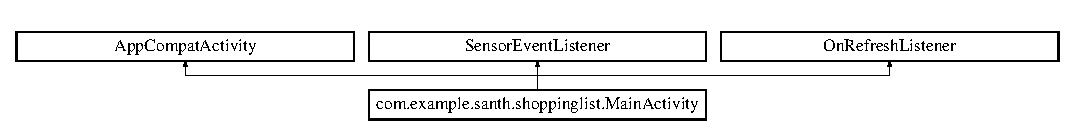
\includegraphics[height=1.377614cm]{classcom_1_1example_1_1santh_1_1shoppinglist_1_1_main_activity}
\end{center}
\end{figure}
\subsection*{Classes}
\begin{DoxyCompactItemize}
\item 
class {\bfseries New\+Sync\+Item}
\item 
class {\bfseries Syncexternal}
\end{DoxyCompactItemize}
\subsection*{Public Member Functions}
\begin{DoxyCompactItemize}
\item 
void \hyperlink{classcom_1_1example_1_1santh_1_1shoppinglist_1_1_main_activity_ac2cdba2d0e75f10c575a579cb0e7e005}{on\+Sensor\+Changed} (Sensor\+Event event)
\begin{DoxyCompactList}\small\item\em Sensor Changed Event to detect Shake of Device . \end{DoxyCompactList}\item 
void \hyperlink{classcom_1_1example_1_1santh_1_1shoppinglist_1_1_main_activity_af24b73687196d9692cda3ec5b9b940b0}{Deletedialog} ()
\begin{DoxyCompactList}\small\item\em Delete Dialog Method for alert box on selecting delete items . \end{DoxyCompactList}\item 
void \hyperlink{classcom_1_1example_1_1santh_1_1shoppinglist_1_1_main_activity_a54421986b1afd82932b0b720bf778e92}{on\+Sensor\+Change} (Sensor\+Event sensor\+Event)
\begin{DoxyCompactList}\small\item\em Implemeting On\+Senor\+Change Method. \end{DoxyCompactList}\item 
void \hyperlink{classcom_1_1example_1_1santh_1_1shoppinglist_1_1_main_activity_a0a919010e14597e55aa8a9e1eb10c623}{on\+Accuracy\+Changed} (Sensor sensor, int accuracy)
\begin{DoxyCompactList}\small\item\em Implementing on\+Accuracy\+Changed method. \end{DoxyCompactList}\item 
boolean \hyperlink{classcom_1_1example_1_1santh_1_1shoppinglist_1_1_main_activity_a27caba662607287a937803ef6f661a1c}{on\+Create\+Options\+Menu} (Menu menu)
\begin{DoxyCompactList}\small\item\em on\+Create\+Options\+Menu Method . \end{DoxyCompactList}\item 
boolean \hyperlink{classcom_1_1example_1_1santh_1_1shoppinglist_1_1_main_activity_a2b96a266ac60b90e48b09d7dc5c7c7a6}{on\+Options\+Item\+Selected} (Menu\+Item item)
\begin{DoxyCompactList}\small\item\em on\+Options\+Item\+Selected Method. \end{DoxyCompactList}\item 
void \hyperlink{classcom_1_1example_1_1santh_1_1shoppinglist_1_1_main_activity_a5b3287fe98bd894937f65cac53aff2f3}{Add\+Item} (View view)
\begin{DoxyCompactList}\small\item\em Add\+Item Method to Add Item to list. \end{DoxyCompactList}\item 
void \hyperlink{classcom_1_1example_1_1santh_1_1shoppinglist_1_1_main_activity_a91d4c9445e987d01d26388181ac32a05}{on\+Voice} (View v)
\begin{DoxyCompactList}\small\item\em on\+Voice Method for Google Sppech to text C\+Onvertor. \end{DoxyCompactList}\item 
void \hyperlink{classcom_1_1example_1_1santh_1_1shoppinglist_1_1_main_activity_a8bfe7142d15e2e78fae9d170da7ae957}{Sync\+Item} (View v)
\item 
void \hyperlink{classcom_1_1example_1_1santh_1_1shoppinglist_1_1_main_activity_a3e4a4b436403fae75ebd98e7f09e230c}{on\+Refresh} ()
\item 
boolean \hyperlink{classcom_1_1example_1_1santh_1_1shoppinglist_1_1_main_activity_aea1441c8e73d0be6fed11c9de2bfa292}{is\+Online} ()
\begin{DoxyCompactList}\small\item\em Determines if the device is internet able. \end{DoxyCompactList}\item 
void \hyperlink{classcom_1_1example_1_1santh_1_1shoppinglist_1_1_main_activity_aea3a89ba2624eed1de56c23664d88ecd}{display\+Data} ()
\begin{DoxyCompactList}\small\item\em Display\+Data Method to Display the items in the List. \end{DoxyCompactList}\end{DoxyCompactItemize}
\subsection*{Public Attributes}
\begin{DoxyCompactItemize}
\item 
Alert\+Dialog \hyperlink{classcom_1_1example_1_1santh_1_1shoppinglist_1_1_main_activity_ab059477f916af817596e0bd4f3f54e29}{my\+Alert\+Dialog}
\item 
Alert\+Dialog \hyperlink{classcom_1_1example_1_1santh_1_1shoppinglist_1_1_main_activity_ae4005027b424faa89a6c20dbf4522901}{my2\+Alert\+Dialog}
\end{DoxyCompactItemize}
\subsection*{Protected Member Functions}
\begin{DoxyCompactItemize}
\item 
void \hyperlink{classcom_1_1example_1_1santh_1_1shoppinglist_1_1_main_activity_a09c4339b395c390420f5a3f5a2ef0e90}{on\+Create} (Bundle saved\+Instance\+State)
\begin{DoxyCompactList}\small\item\em on\+Create Method in Main Activity \end{DoxyCompactList}\item 
void \hyperlink{classcom_1_1example_1_1santh_1_1shoppinglist_1_1_main_activity_a6567abea3528c5e3e3e523ecead734c8}{on\+Pause} ()
\begin{DoxyCompactList}\small\item\em on\+Pause method to pause the sensor\+Manager \end{DoxyCompactList}\item 
void \hyperlink{classcom_1_1example_1_1santh_1_1shoppinglist_1_1_main_activity_aadfa7e9478d4a45e273f9ccbc8539100}{on\+Destroy} ()
\begin{DoxyCompactList}\small\item\em on\+Destroy Method . \end{DoxyCompactList}\item 
void \hyperlink{classcom_1_1example_1_1santh_1_1shoppinglist_1_1_main_activity_a2e421cbd8b1ce8efc186b39fdca245ac}{on\+Resume} ()
\begin{DoxyCompactList}\small\item\em on\+Resume Method for resuming the sensor \end{DoxyCompactList}\item 
void \hyperlink{classcom_1_1example_1_1santh_1_1shoppinglist_1_1_main_activity_abbd9519fe806e438184036e3e450ea11}{on\+Activity\+Result} (int request\+Code, int result\+Code, Intent data)
\begin{DoxyCompactList}\small\item\em on\+Activity\+Result method to retrieve Item\+Name from Google voice. \end{DoxyCompactList}\end{DoxyCompactItemize}
\subsection*{Static Protected Attributes}
\begin{DoxyCompactItemize}
\item 
static final int \hyperlink{classcom_1_1example_1_1santh_1_1shoppinglist_1_1_main_activity_a4f358ad66f8020173b2bac71b406a1d5}{R\+E\+S\+U\+L\+T\+\_\+\+S\+P\+E\+E\+CH} = 1
\end{DoxyCompactItemize}


\subsection{Detailed Description}
Begin of class Main\+Activty where List names and its corresponding features are shown. 

Functionalities include adding ,editing and deleting List. 

\subsection{Member Function Documentation}
\index{com\+::example\+::santh\+::shoppinglist\+::\+Main\+Activity@{com\+::example\+::santh\+::shoppinglist\+::\+Main\+Activity}!Add\+Item@{Add\+Item}}
\index{Add\+Item@{Add\+Item}!com\+::example\+::santh\+::shoppinglist\+::\+Main\+Activity@{com\+::example\+::santh\+::shoppinglist\+::\+Main\+Activity}}
\subsubsection[{\texorpdfstring{Add\+Item(\+View view)}{AddItem(View view)}}]{\setlength{\rightskip}{0pt plus 5cm}void com.\+example.\+santh.\+shoppinglist.\+Main\+Activity.\+Add\+Item (
\begin{DoxyParamCaption}
\item[{View}]{view}
\end{DoxyParamCaption}
)}\hypertarget{classcom_1_1example_1_1santh_1_1shoppinglist_1_1_main_activity_a5b3287fe98bd894937f65cac53aff2f3}{}\label{classcom_1_1example_1_1santh_1_1shoppinglist_1_1_main_activity_a5b3287fe98bd894937f65cac53aff2f3}


Add\+Item Method to Add Item to list. 


\begin{DoxyParams}{Parameters}
{\em view} & \\
\hline
\end{DoxyParams}
\index{com\+::example\+::santh\+::shoppinglist\+::\+Main\+Activity@{com\+::example\+::santh\+::shoppinglist\+::\+Main\+Activity}!Deletedialog@{Deletedialog}}
\index{Deletedialog@{Deletedialog}!com\+::example\+::santh\+::shoppinglist\+::\+Main\+Activity@{com\+::example\+::santh\+::shoppinglist\+::\+Main\+Activity}}
\subsubsection[{\texorpdfstring{Deletedialog()}{Deletedialog()}}]{\setlength{\rightskip}{0pt plus 5cm}void com.\+example.\+santh.\+shoppinglist.\+Main\+Activity.\+Deletedialog (
\begin{DoxyParamCaption}
{}
\end{DoxyParamCaption}
)}\hypertarget{classcom_1_1example_1_1santh_1_1shoppinglist_1_1_main_activity_af24b73687196d9692cda3ec5b9b940b0}{}\label{classcom_1_1example_1_1santh_1_1shoppinglist_1_1_main_activity_af24b73687196d9692cda3ec5b9b940b0}


Delete Dialog Method for alert box on selecting delete items . 

\index{com\+::example\+::santh\+::shoppinglist\+::\+Main\+Activity@{com\+::example\+::santh\+::shoppinglist\+::\+Main\+Activity}!display\+Data@{display\+Data}}
\index{display\+Data@{display\+Data}!com\+::example\+::santh\+::shoppinglist\+::\+Main\+Activity@{com\+::example\+::santh\+::shoppinglist\+::\+Main\+Activity}}
\subsubsection[{\texorpdfstring{display\+Data()}{displayData()}}]{\setlength{\rightskip}{0pt plus 5cm}void com.\+example.\+santh.\+shoppinglist.\+Main\+Activity.\+display\+Data (
\begin{DoxyParamCaption}
{}
\end{DoxyParamCaption}
)}\hypertarget{classcom_1_1example_1_1santh_1_1shoppinglist_1_1_main_activity_aea3a89ba2624eed1de56c23664d88ecd}{}\label{classcom_1_1example_1_1santh_1_1shoppinglist_1_1_main_activity_aea3a89ba2624eed1de56c23664d88ecd}


Display\+Data Method to Display the items in the List. 

\index{com\+::example\+::santh\+::shoppinglist\+::\+Main\+Activity@{com\+::example\+::santh\+::shoppinglist\+::\+Main\+Activity}!is\+Online@{is\+Online}}
\index{is\+Online@{is\+Online}!com\+::example\+::santh\+::shoppinglist\+::\+Main\+Activity@{com\+::example\+::santh\+::shoppinglist\+::\+Main\+Activity}}
\subsubsection[{\texorpdfstring{is\+Online()}{isOnline()}}]{\setlength{\rightskip}{0pt plus 5cm}boolean com.\+example.\+santh.\+shoppinglist.\+Main\+Activity.\+is\+Online (
\begin{DoxyParamCaption}
{}
\end{DoxyParamCaption}
)}\hypertarget{classcom_1_1example_1_1santh_1_1shoppinglist_1_1_main_activity_aea1441c8e73d0be6fed11c9de2bfa292}{}\label{classcom_1_1example_1_1santh_1_1shoppinglist_1_1_main_activity_aea1441c8e73d0be6fed11c9de2bfa292}


Determines if the device is internet able. 

\index{com\+::example\+::santh\+::shoppinglist\+::\+Main\+Activity@{com\+::example\+::santh\+::shoppinglist\+::\+Main\+Activity}!on\+Accuracy\+Changed@{on\+Accuracy\+Changed}}
\index{on\+Accuracy\+Changed@{on\+Accuracy\+Changed}!com\+::example\+::santh\+::shoppinglist\+::\+Main\+Activity@{com\+::example\+::santh\+::shoppinglist\+::\+Main\+Activity}}
\subsubsection[{\texorpdfstring{on\+Accuracy\+Changed(\+Sensor sensor, int accuracy)}{onAccuracyChanged(Sensor sensor, int accuracy)}}]{\setlength{\rightskip}{0pt plus 5cm}void com.\+example.\+santh.\+shoppinglist.\+Main\+Activity.\+on\+Accuracy\+Changed (
\begin{DoxyParamCaption}
\item[{Sensor}]{sensor, }
\item[{int}]{accuracy}
\end{DoxyParamCaption}
)}\hypertarget{classcom_1_1example_1_1santh_1_1shoppinglist_1_1_main_activity_a0a919010e14597e55aa8a9e1eb10c623}{}\label{classcom_1_1example_1_1santh_1_1shoppinglist_1_1_main_activity_a0a919010e14597e55aa8a9e1eb10c623}


Implementing on\+Accuracy\+Changed method. 


\begin{DoxyParams}{Parameters}
{\em sensor} & \\
\hline
{\em accuracy} & \\
\hline
\end{DoxyParams}
\index{com\+::example\+::santh\+::shoppinglist\+::\+Main\+Activity@{com\+::example\+::santh\+::shoppinglist\+::\+Main\+Activity}!on\+Activity\+Result@{on\+Activity\+Result}}
\index{on\+Activity\+Result@{on\+Activity\+Result}!com\+::example\+::santh\+::shoppinglist\+::\+Main\+Activity@{com\+::example\+::santh\+::shoppinglist\+::\+Main\+Activity}}
\subsubsection[{\texorpdfstring{on\+Activity\+Result(int request\+Code, int result\+Code, Intent data)}{onActivityResult(int requestCode, int resultCode, Intent data)}}]{\setlength{\rightskip}{0pt plus 5cm}void com.\+example.\+santh.\+shoppinglist.\+Main\+Activity.\+on\+Activity\+Result (
\begin{DoxyParamCaption}
\item[{int}]{request\+Code, }
\item[{int}]{result\+Code, }
\item[{Intent}]{data}
\end{DoxyParamCaption}
)\hspace{0.3cm}{\ttfamily [protected]}}\hypertarget{classcom_1_1example_1_1santh_1_1shoppinglist_1_1_main_activity_abbd9519fe806e438184036e3e450ea11}{}\label{classcom_1_1example_1_1santh_1_1shoppinglist_1_1_main_activity_abbd9519fe806e438184036e3e450ea11}


on\+Activity\+Result method to retrieve Item\+Name from Google voice. 


\begin{DoxyParams}{Parameters}
{\em request\+Code} & \\
\hline
{\em result\+Code} & \\
\hline
{\em data} & \\
\hline
\end{DoxyParams}
\index{com\+::example\+::santh\+::shoppinglist\+::\+Main\+Activity@{com\+::example\+::santh\+::shoppinglist\+::\+Main\+Activity}!on\+Create@{on\+Create}}
\index{on\+Create@{on\+Create}!com\+::example\+::santh\+::shoppinglist\+::\+Main\+Activity@{com\+::example\+::santh\+::shoppinglist\+::\+Main\+Activity}}
\subsubsection[{\texorpdfstring{on\+Create(\+Bundle saved\+Instance\+State)}{onCreate(Bundle savedInstanceState)}}]{\setlength{\rightskip}{0pt plus 5cm}void com.\+example.\+santh.\+shoppinglist.\+Main\+Activity.\+on\+Create (
\begin{DoxyParamCaption}
\item[{Bundle}]{saved\+Instance\+State}
\end{DoxyParamCaption}
)\hspace{0.3cm}{\ttfamily [protected]}}\hypertarget{classcom_1_1example_1_1santh_1_1shoppinglist_1_1_main_activity_a09c4339b395c390420f5a3f5a2ef0e90}{}\label{classcom_1_1example_1_1santh_1_1shoppinglist_1_1_main_activity_a09c4339b395c390420f5a3f5a2ef0e90}


on\+Create Method in Main Activity 


\begin{DoxyParams}{Parameters}
{\em saved\+Instance\+State} & \\
\hline
\end{DoxyParams}
Set Actionbar

create Instance for Sensor and Sensor\+Manager

Create an object instance for DB Helper Class

Set Scrollview for Listview \index{com\+::example\+::santh\+::shoppinglist\+::\+Main\+Activity@{com\+::example\+::santh\+::shoppinglist\+::\+Main\+Activity}!on\+Create\+Options\+Menu@{on\+Create\+Options\+Menu}}
\index{on\+Create\+Options\+Menu@{on\+Create\+Options\+Menu}!com\+::example\+::santh\+::shoppinglist\+::\+Main\+Activity@{com\+::example\+::santh\+::shoppinglist\+::\+Main\+Activity}}
\subsubsection[{\texorpdfstring{on\+Create\+Options\+Menu(\+Menu menu)}{onCreateOptionsMenu(Menu menu)}}]{\setlength{\rightskip}{0pt plus 5cm}boolean com.\+example.\+santh.\+shoppinglist.\+Main\+Activity.\+on\+Create\+Options\+Menu (
\begin{DoxyParamCaption}
\item[{Menu}]{menu}
\end{DoxyParamCaption}
)}\hypertarget{classcom_1_1example_1_1santh_1_1shoppinglist_1_1_main_activity_a27caba662607287a937803ef6f661a1c}{}\label{classcom_1_1example_1_1santh_1_1shoppinglist_1_1_main_activity_a27caba662607287a937803ef6f661a1c}


on\+Create\+Options\+Menu Method . 

Inflate the menu; this adds items to the action bar if it is present. 
\begin{DoxyParams}{Parameters}
{\em menu} & \\
\hline
\end{DoxyParams}
\begin{DoxyReturn}{Returns}

\end{DoxyReturn}
\index{com\+::example\+::santh\+::shoppinglist\+::\+Main\+Activity@{com\+::example\+::santh\+::shoppinglist\+::\+Main\+Activity}!on\+Destroy@{on\+Destroy}}
\index{on\+Destroy@{on\+Destroy}!com\+::example\+::santh\+::shoppinglist\+::\+Main\+Activity@{com\+::example\+::santh\+::shoppinglist\+::\+Main\+Activity}}
\subsubsection[{\texorpdfstring{on\+Destroy()}{onDestroy()}}]{\setlength{\rightskip}{0pt plus 5cm}void com.\+example.\+santh.\+shoppinglist.\+Main\+Activity.\+on\+Destroy (
\begin{DoxyParamCaption}
{}
\end{DoxyParamCaption}
)\hspace{0.3cm}{\ttfamily [protected]}}\hypertarget{classcom_1_1example_1_1santh_1_1shoppinglist_1_1_main_activity_aadfa7e9478d4a45e273f9ccbc8539100}{}\label{classcom_1_1example_1_1santh_1_1shoppinglist_1_1_main_activity_aadfa7e9478d4a45e273f9ccbc8539100}


on\+Destroy Method . 

\index{com\+::example\+::santh\+::shoppinglist\+::\+Main\+Activity@{com\+::example\+::santh\+::shoppinglist\+::\+Main\+Activity}!on\+Options\+Item\+Selected@{on\+Options\+Item\+Selected}}
\index{on\+Options\+Item\+Selected@{on\+Options\+Item\+Selected}!com\+::example\+::santh\+::shoppinglist\+::\+Main\+Activity@{com\+::example\+::santh\+::shoppinglist\+::\+Main\+Activity}}
\subsubsection[{\texorpdfstring{on\+Options\+Item\+Selected(\+Menu\+Item item)}{onOptionsItemSelected(MenuItem item)}}]{\setlength{\rightskip}{0pt plus 5cm}boolean com.\+example.\+santh.\+shoppinglist.\+Main\+Activity.\+on\+Options\+Item\+Selected (
\begin{DoxyParamCaption}
\item[{Menu\+Item}]{item}
\end{DoxyParamCaption}
)}\hypertarget{classcom_1_1example_1_1santh_1_1shoppinglist_1_1_main_activity_a2b96a266ac60b90e48b09d7dc5c7c7a6}{}\label{classcom_1_1example_1_1santh_1_1shoppinglist_1_1_main_activity_a2b96a266ac60b90e48b09d7dc5c7c7a6}


on\+Options\+Item\+Selected Method. 

Handle action bar item clicks here. The action bar will automatically handle clicks on the Home/\+Up button, so long as you specify a parent activity in Android\+Manifest.\+xml. 
\begin{DoxyParams}{Parameters}
{\em item} & \\
\hline
\end{DoxyParams}
\begin{DoxyReturn}{Returns}

\end{DoxyReturn}
\index{com\+::example\+::santh\+::shoppinglist\+::\+Main\+Activity@{com\+::example\+::santh\+::shoppinglist\+::\+Main\+Activity}!on\+Pause@{on\+Pause}}
\index{on\+Pause@{on\+Pause}!com\+::example\+::santh\+::shoppinglist\+::\+Main\+Activity@{com\+::example\+::santh\+::shoppinglist\+::\+Main\+Activity}}
\subsubsection[{\texorpdfstring{on\+Pause()}{onPause()}}]{\setlength{\rightskip}{0pt plus 5cm}void com.\+example.\+santh.\+shoppinglist.\+Main\+Activity.\+on\+Pause (
\begin{DoxyParamCaption}
{}
\end{DoxyParamCaption}
)\hspace{0.3cm}{\ttfamily [protected]}}\hypertarget{classcom_1_1example_1_1santh_1_1shoppinglist_1_1_main_activity_a6567abea3528c5e3e3e523ecead734c8}{}\label{classcom_1_1example_1_1santh_1_1shoppinglist_1_1_main_activity_a6567abea3528c5e3e3e523ecead734c8}


on\+Pause method to pause the sensor\+Manager 

\index{com\+::example\+::santh\+::shoppinglist\+::\+Main\+Activity@{com\+::example\+::santh\+::shoppinglist\+::\+Main\+Activity}!on\+Refresh@{on\+Refresh}}
\index{on\+Refresh@{on\+Refresh}!com\+::example\+::santh\+::shoppinglist\+::\+Main\+Activity@{com\+::example\+::santh\+::shoppinglist\+::\+Main\+Activity}}
\subsubsection[{\texorpdfstring{on\+Refresh()}{onRefresh()}}]{\setlength{\rightskip}{0pt plus 5cm}void com.\+example.\+santh.\+shoppinglist.\+Main\+Activity.\+on\+Refresh (
\begin{DoxyParamCaption}
{}
\end{DoxyParamCaption}
)}\hypertarget{classcom_1_1example_1_1santh_1_1shoppinglist_1_1_main_activity_a3e4a4b436403fae75ebd98e7f09e230c}{}\label{classcom_1_1example_1_1santh_1_1shoppinglist_1_1_main_activity_a3e4a4b436403fae75ebd98e7f09e230c}
\index{com\+::example\+::santh\+::shoppinglist\+::\+Main\+Activity@{com\+::example\+::santh\+::shoppinglist\+::\+Main\+Activity}!on\+Resume@{on\+Resume}}
\index{on\+Resume@{on\+Resume}!com\+::example\+::santh\+::shoppinglist\+::\+Main\+Activity@{com\+::example\+::santh\+::shoppinglist\+::\+Main\+Activity}}
\subsubsection[{\texorpdfstring{on\+Resume()}{onResume()}}]{\setlength{\rightskip}{0pt plus 5cm}void com.\+example.\+santh.\+shoppinglist.\+Main\+Activity.\+on\+Resume (
\begin{DoxyParamCaption}
{}
\end{DoxyParamCaption}
)\hspace{0.3cm}{\ttfamily [protected]}}\hypertarget{classcom_1_1example_1_1santh_1_1shoppinglist_1_1_main_activity_a2e421cbd8b1ce8efc186b39fdca245ac}{}\label{classcom_1_1example_1_1santh_1_1shoppinglist_1_1_main_activity_a2e421cbd8b1ce8efc186b39fdca245ac}


on\+Resume Method for resuming the sensor 

\index{com\+::example\+::santh\+::shoppinglist\+::\+Main\+Activity@{com\+::example\+::santh\+::shoppinglist\+::\+Main\+Activity}!on\+Sensor\+Change@{on\+Sensor\+Change}}
\index{on\+Sensor\+Change@{on\+Sensor\+Change}!com\+::example\+::santh\+::shoppinglist\+::\+Main\+Activity@{com\+::example\+::santh\+::shoppinglist\+::\+Main\+Activity}}
\subsubsection[{\texorpdfstring{on\+Sensor\+Change(\+Sensor\+Event sensor\+Event)}{onSensorChange(SensorEvent sensorEvent)}}]{\setlength{\rightskip}{0pt plus 5cm}void com.\+example.\+santh.\+shoppinglist.\+Main\+Activity.\+on\+Sensor\+Change (
\begin{DoxyParamCaption}
\item[{Sensor\+Event}]{sensor\+Event}
\end{DoxyParamCaption}
)}\hypertarget{classcom_1_1example_1_1santh_1_1shoppinglist_1_1_main_activity_a54421986b1afd82932b0b720bf778e92}{}\label{classcom_1_1example_1_1santh_1_1shoppinglist_1_1_main_activity_a54421986b1afd82932b0b720bf778e92}


Implemeting On\+Senor\+Change Method. 


\begin{DoxyParams}{Parameters}
{\em sensor\+Event} & \\
\hline
\end{DoxyParams}
\index{com\+::example\+::santh\+::shoppinglist\+::\+Main\+Activity@{com\+::example\+::santh\+::shoppinglist\+::\+Main\+Activity}!on\+Sensor\+Changed@{on\+Sensor\+Changed}}
\index{on\+Sensor\+Changed@{on\+Sensor\+Changed}!com\+::example\+::santh\+::shoppinglist\+::\+Main\+Activity@{com\+::example\+::santh\+::shoppinglist\+::\+Main\+Activity}}
\subsubsection[{\texorpdfstring{on\+Sensor\+Changed(\+Sensor\+Event event)}{onSensorChanged(SensorEvent event)}}]{\setlength{\rightskip}{0pt plus 5cm}void com.\+example.\+santh.\+shoppinglist.\+Main\+Activity.\+on\+Sensor\+Changed (
\begin{DoxyParamCaption}
\item[{Sensor\+Event}]{event}
\end{DoxyParamCaption}
)}\hypertarget{classcom_1_1example_1_1santh_1_1shoppinglist_1_1_main_activity_ac2cdba2d0e75f10c575a579cb0e7e005}{}\label{classcom_1_1example_1_1santh_1_1shoppinglist_1_1_main_activity_ac2cdba2d0e75f10c575a579cb0e7e005}


Sensor Changed Event to detect Shake of Device . 


\begin{DoxyParams}{Parameters}
{\em event} & \\
\hline
\end{DoxyParams}
\index{com\+::example\+::santh\+::shoppinglist\+::\+Main\+Activity@{com\+::example\+::santh\+::shoppinglist\+::\+Main\+Activity}!on\+Voice@{on\+Voice}}
\index{on\+Voice@{on\+Voice}!com\+::example\+::santh\+::shoppinglist\+::\+Main\+Activity@{com\+::example\+::santh\+::shoppinglist\+::\+Main\+Activity}}
\subsubsection[{\texorpdfstring{on\+Voice(\+View v)}{onVoice(View v)}}]{\setlength{\rightskip}{0pt plus 5cm}void com.\+example.\+santh.\+shoppinglist.\+Main\+Activity.\+on\+Voice (
\begin{DoxyParamCaption}
\item[{View}]{v}
\end{DoxyParamCaption}
)}\hypertarget{classcom_1_1example_1_1santh_1_1shoppinglist_1_1_main_activity_a91d4c9445e987d01d26388181ac32a05}{}\label{classcom_1_1example_1_1santh_1_1shoppinglist_1_1_main_activity_a91d4c9445e987d01d26388181ac32a05}


on\+Voice Method for Google Sppech to text C\+Onvertor. 


\begin{DoxyParams}{Parameters}
{\em v} & \\
\hline
\end{DoxyParams}
\index{com\+::example\+::santh\+::shoppinglist\+::\+Main\+Activity@{com\+::example\+::santh\+::shoppinglist\+::\+Main\+Activity}!Sync\+Item@{Sync\+Item}}
\index{Sync\+Item@{Sync\+Item}!com\+::example\+::santh\+::shoppinglist\+::\+Main\+Activity@{com\+::example\+::santh\+::shoppinglist\+::\+Main\+Activity}}
\subsubsection[{\texorpdfstring{Sync\+Item(\+View v)}{SyncItem(View v)}}]{\setlength{\rightskip}{0pt plus 5cm}void com.\+example.\+santh.\+shoppinglist.\+Main\+Activity.\+Sync\+Item (
\begin{DoxyParamCaption}
\item[{View}]{v}
\end{DoxyParamCaption}
)}\hypertarget{classcom_1_1example_1_1santh_1_1shoppinglist_1_1_main_activity_a8bfe7142d15e2e78fae9d170da7ae957}{}\label{classcom_1_1example_1_1santh_1_1shoppinglist_1_1_main_activity_a8bfe7142d15e2e78fae9d170da7ae957}


\subsection{Member Data Documentation}
\index{com\+::example\+::santh\+::shoppinglist\+::\+Main\+Activity@{com\+::example\+::santh\+::shoppinglist\+::\+Main\+Activity}!my2\+Alert\+Dialog@{my2\+Alert\+Dialog}}
\index{my2\+Alert\+Dialog@{my2\+Alert\+Dialog}!com\+::example\+::santh\+::shoppinglist\+::\+Main\+Activity@{com\+::example\+::santh\+::shoppinglist\+::\+Main\+Activity}}
\subsubsection[{\texorpdfstring{my2\+Alert\+Dialog}{my2AlertDialog}}]{\setlength{\rightskip}{0pt plus 5cm}Alert\+Dialog com.\+example.\+santh.\+shoppinglist.\+Main\+Activity.\+my2\+Alert\+Dialog}\hypertarget{classcom_1_1example_1_1santh_1_1shoppinglist_1_1_main_activity_ae4005027b424faa89a6c20dbf4522901}{}\label{classcom_1_1example_1_1santh_1_1shoppinglist_1_1_main_activity_ae4005027b424faa89a6c20dbf4522901}
\index{com\+::example\+::santh\+::shoppinglist\+::\+Main\+Activity@{com\+::example\+::santh\+::shoppinglist\+::\+Main\+Activity}!my\+Alert\+Dialog@{my\+Alert\+Dialog}}
\index{my\+Alert\+Dialog@{my\+Alert\+Dialog}!com\+::example\+::santh\+::shoppinglist\+::\+Main\+Activity@{com\+::example\+::santh\+::shoppinglist\+::\+Main\+Activity}}
\subsubsection[{\texorpdfstring{my\+Alert\+Dialog}{myAlertDialog}}]{\setlength{\rightskip}{0pt plus 5cm}Alert\+Dialog com.\+example.\+santh.\+shoppinglist.\+Main\+Activity.\+my\+Alert\+Dialog}\hypertarget{classcom_1_1example_1_1santh_1_1shoppinglist_1_1_main_activity_ab059477f916af817596e0bd4f3f54e29}{}\label{classcom_1_1example_1_1santh_1_1shoppinglist_1_1_main_activity_ab059477f916af817596e0bd4f3f54e29}
\index{com\+::example\+::santh\+::shoppinglist\+::\+Main\+Activity@{com\+::example\+::santh\+::shoppinglist\+::\+Main\+Activity}!R\+E\+S\+U\+L\+T\+\_\+\+S\+P\+E\+E\+CH@{R\+E\+S\+U\+L\+T\+\_\+\+S\+P\+E\+E\+CH}}
\index{R\+E\+S\+U\+L\+T\+\_\+\+S\+P\+E\+E\+CH@{R\+E\+S\+U\+L\+T\+\_\+\+S\+P\+E\+E\+CH}!com\+::example\+::santh\+::shoppinglist\+::\+Main\+Activity@{com\+::example\+::santh\+::shoppinglist\+::\+Main\+Activity}}
\subsubsection[{\texorpdfstring{R\+E\+S\+U\+L\+T\+\_\+\+S\+P\+E\+E\+CH}{RESULT_SPEECH}}]{\setlength{\rightskip}{0pt plus 5cm}final int com.\+example.\+santh.\+shoppinglist.\+Main\+Activity.\+R\+E\+S\+U\+L\+T\+\_\+\+S\+P\+E\+E\+CH = 1\hspace{0.3cm}{\ttfamily [static]}, {\ttfamily [protected]}}\hypertarget{classcom_1_1example_1_1santh_1_1shoppinglist_1_1_main_activity_a4f358ad66f8020173b2bac71b406a1d5}{}\label{classcom_1_1example_1_1santh_1_1shoppinglist_1_1_main_activity_a4f358ad66f8020173b2bac71b406a1d5}


The documentation for this class was generated from the following file\+:\begin{DoxyCompactItemize}
\item 
E\+:/\+Android/\+Shopping\+List\+D\+B4 2/app/src/main/java/com/example/santh/shoppinglist/\hyperlink{_main_activity_8java}{Main\+Activity.\+java}\end{DoxyCompactItemize}

\hypertarget{classcom_1_1example_1_1santh_1_1shoppinglist_1_1_my_custom_adapter}{}\section{com.\+example.\+santh.\+shoppinglist.\+My\+Custom\+Adapter Class Reference}
\label{classcom_1_1example_1_1santh_1_1shoppinglist_1_1_my_custom_adapter}\index{com.\+example.\+santh.\+shoppinglist.\+My\+Custom\+Adapter@{com.\+example.\+santh.\+shoppinglist.\+My\+Custom\+Adapter}}


My Custom\+Adapter Class to display all item information.\+It uses four text views Itemname ,Quantity, price,comments The inflater layout has these four Text views which are binded in this adapter class.  


Inheritance diagram for com.\+example.\+santh.\+shoppinglist.\+My\+Custom\+Adapter\+:\begin{figure}[H]
\begin{center}
\leavevmode
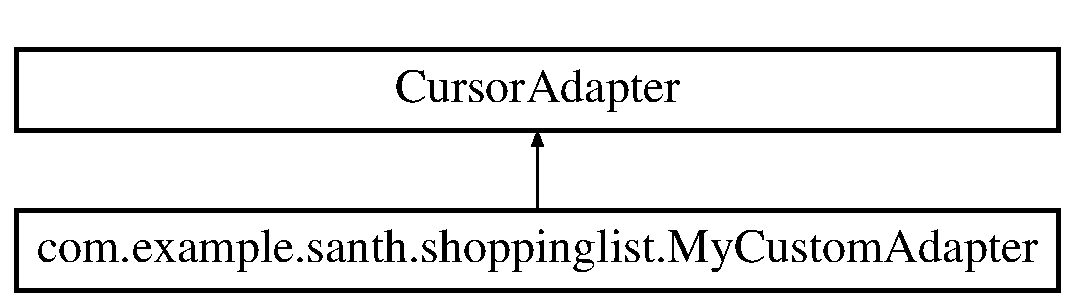
\includegraphics[height=2.000000cm]{classcom_1_1example_1_1santh_1_1shoppinglist_1_1_my_custom_adapter}
\end{center}
\end{figure}
\subsection*{Public Member Functions}
\begin{DoxyCompactItemize}
\item 
\hyperlink{classcom_1_1example_1_1santh_1_1shoppinglist_1_1_my_custom_adapter_a5f294d42d4509ab9b456a4a756a01390}{My\+Custom\+Adapter} (Context context, Cursor c)
\begin{DoxyCompactList}\small\item\em Constructor function for My\+Customadapter. \end{DoxyCompactList}\item 
View \hyperlink{classcom_1_1example_1_1santh_1_1shoppinglist_1_1_my_custom_adapter_ab62e3e7040d84494b8e1c90812aad581}{new\+View} (final Context context, final Cursor cursor, View\+Group parent)
\begin{DoxyCompactList}\small\item\em Attaching View to the Adapter. \end{DoxyCompactList}\item 
long \hyperlink{classcom_1_1example_1_1santh_1_1shoppinglist_1_1_my_custom_adapter_ab8529e9563ccab567daf7a7467a95eb1}{get\+Item\+Id} (int pos)
\item 
void \hyperlink{classcom_1_1example_1_1santh_1_1shoppinglist_1_1_my_custom_adapter_a7f9fb1e4d114f98be51aa8b76899d740}{bind\+View} (View v, final Context context, final Cursor c)
\begin{DoxyCompactList}\small\item\em Bind View to Layout. \end{DoxyCompactList}\end{DoxyCompactItemize}


\subsection{Detailed Description}
My Custom\+Adapter Class to display all item information.\+It uses four text views Itemname ,Quantity, price,comments The inflater layout has these four Text views which are binded in this adapter class. 

\subsection{Constructor \& Destructor Documentation}
\index{com\+::example\+::santh\+::shoppinglist\+::\+My\+Custom\+Adapter@{com\+::example\+::santh\+::shoppinglist\+::\+My\+Custom\+Adapter}!My\+Custom\+Adapter@{My\+Custom\+Adapter}}
\index{My\+Custom\+Adapter@{My\+Custom\+Adapter}!com\+::example\+::santh\+::shoppinglist\+::\+My\+Custom\+Adapter@{com\+::example\+::santh\+::shoppinglist\+::\+My\+Custom\+Adapter}}
\subsubsection[{\texorpdfstring{My\+Custom\+Adapter(\+Context context, Cursor c)}{MyCustomAdapter(Context context, Cursor c)}}]{\setlength{\rightskip}{0pt plus 5cm}com.\+example.\+santh.\+shoppinglist.\+My\+Custom\+Adapter.\+My\+Custom\+Adapter (
\begin{DoxyParamCaption}
\item[{Context}]{context, }
\item[{Cursor}]{c}
\end{DoxyParamCaption}
)}\hypertarget{classcom_1_1example_1_1santh_1_1shoppinglist_1_1_my_custom_adapter_a5f294d42d4509ab9b456a4a756a01390}{}\label{classcom_1_1example_1_1santh_1_1shoppinglist_1_1_my_custom_adapter_a5f294d42d4509ab9b456a4a756a01390}


Constructor function for My\+Customadapter. 


\begin{DoxyParams}{Parameters}
{\em context} & \\
\hline
{\em c} & \\
\hline
\end{DoxyParams}


\subsection{Member Function Documentation}
\index{com\+::example\+::santh\+::shoppinglist\+::\+My\+Custom\+Adapter@{com\+::example\+::santh\+::shoppinglist\+::\+My\+Custom\+Adapter}!bind\+View@{bind\+View}}
\index{bind\+View@{bind\+View}!com\+::example\+::santh\+::shoppinglist\+::\+My\+Custom\+Adapter@{com\+::example\+::santh\+::shoppinglist\+::\+My\+Custom\+Adapter}}
\subsubsection[{\texorpdfstring{bind\+View(\+View v, final Context context, final Cursor c)}{bindView(View v, final Context context, final Cursor c)}}]{\setlength{\rightskip}{0pt plus 5cm}void com.\+example.\+santh.\+shoppinglist.\+My\+Custom\+Adapter.\+bind\+View (
\begin{DoxyParamCaption}
\item[{View}]{v, }
\item[{final Context}]{context, }
\item[{final Cursor}]{c}
\end{DoxyParamCaption}
)}\hypertarget{classcom_1_1example_1_1santh_1_1shoppinglist_1_1_my_custom_adapter_a7f9fb1e4d114f98be51aa8b76899d740}{}\label{classcom_1_1example_1_1santh_1_1shoppinglist_1_1_my_custom_adapter_a7f9fb1e4d114f98be51aa8b76899d740}


Bind View to Layout. 

\begin{DoxyAuthor}{Author}
will
\end{DoxyAuthor}

\begin{DoxyParams}{Parameters}
{\em v} & The view in which the elements we set up here will be displayed.\\
\hline
{\em context} & The running context where this List\+View adapter will be active.\\
\hline
{\em c} & The Cursor containing the query results we will display.\\
\hline
{\em v} & \\
\hline
{\em context} & \\
\hline
{\em c} & \\
\hline
\end{DoxyParams}
Next set the title of the entry.

Set Date

Decide if we should display the deletion indicator\index{com\+::example\+::santh\+::shoppinglist\+::\+My\+Custom\+Adapter@{com\+::example\+::santh\+::shoppinglist\+::\+My\+Custom\+Adapter}!get\+Item\+Id@{get\+Item\+Id}}
\index{get\+Item\+Id@{get\+Item\+Id}!com\+::example\+::santh\+::shoppinglist\+::\+My\+Custom\+Adapter@{com\+::example\+::santh\+::shoppinglist\+::\+My\+Custom\+Adapter}}
\subsubsection[{\texorpdfstring{get\+Item\+Id(int pos)}{getItemId(int pos)}}]{\setlength{\rightskip}{0pt plus 5cm}long com.\+example.\+santh.\+shoppinglist.\+My\+Custom\+Adapter.\+get\+Item\+Id (
\begin{DoxyParamCaption}
\item[{int}]{pos}
\end{DoxyParamCaption}
)}\hypertarget{classcom_1_1example_1_1santh_1_1shoppinglist_1_1_my_custom_adapter_ab8529e9563ccab567daf7a7467a95eb1}{}\label{classcom_1_1example_1_1santh_1_1shoppinglist_1_1_my_custom_adapter_ab8529e9563ccab567daf7a7467a95eb1}
\index{com\+::example\+::santh\+::shoppinglist\+::\+My\+Custom\+Adapter@{com\+::example\+::santh\+::shoppinglist\+::\+My\+Custom\+Adapter}!new\+View@{new\+View}}
\index{new\+View@{new\+View}!com\+::example\+::santh\+::shoppinglist\+::\+My\+Custom\+Adapter@{com\+::example\+::santh\+::shoppinglist\+::\+My\+Custom\+Adapter}}
\subsubsection[{\texorpdfstring{new\+View(final Context context, final Cursor cursor, View\+Group parent)}{newView(final Context context, final Cursor cursor, ViewGroup parent)}}]{\setlength{\rightskip}{0pt plus 5cm}View com.\+example.\+santh.\+shoppinglist.\+My\+Custom\+Adapter.\+new\+View (
\begin{DoxyParamCaption}
\item[{final Context}]{context, }
\item[{final Cursor}]{cursor, }
\item[{View\+Group}]{parent}
\end{DoxyParamCaption}
)}\hypertarget{classcom_1_1example_1_1santh_1_1shoppinglist_1_1_my_custom_adapter_ab62e3e7040d84494b8e1c90812aad581}{}\label{classcom_1_1example_1_1santh_1_1shoppinglist_1_1_my_custom_adapter_ab62e3e7040d84494b8e1c90812aad581}


Attaching View to the Adapter. 


\begin{DoxyParams}{Parameters}
{\em context} & \\
\hline
{\em cursor} & \\
\hline
{\em parent} & \\
\hline
\end{DoxyParams}
\begin{DoxyReturn}{Returns}

\end{DoxyReturn}


The documentation for this class was generated from the following file\+:\begin{DoxyCompactItemize}
\item 
E\+:/\+Android/\+Shopping\+List\+D\+B4 2/app/src/main/java/com/example/santh/shoppinglist/\hyperlink{_my_custom_adapter_8java}{My\+Custom\+Adapter.\+java}\end{DoxyCompactItemize}

\hypertarget{classcom_1_1example_1_1santh_1_1shoppinglist_1_1new_list_adapter}{}\section{com.\+example.\+santh.\+shoppinglist.\+new\+List\+Adapter Class Reference}
\label{classcom_1_1example_1_1santh_1_1shoppinglist_1_1new_list_adapter}\index{com.\+example.\+santh.\+shoppinglist.\+new\+List\+Adapter@{com.\+example.\+santh.\+shoppinglist.\+new\+List\+Adapter}}


New\+List\+Adapter Class to Display List name and other parameters .It uses four text view Listname ,Date,List price and count of purchased items/\+Un\+Purchaseditems.  


Inheritance diagram for com.\+example.\+santh.\+shoppinglist.\+new\+List\+Adapter\+:\begin{figure}[H]
\begin{center}
\leavevmode
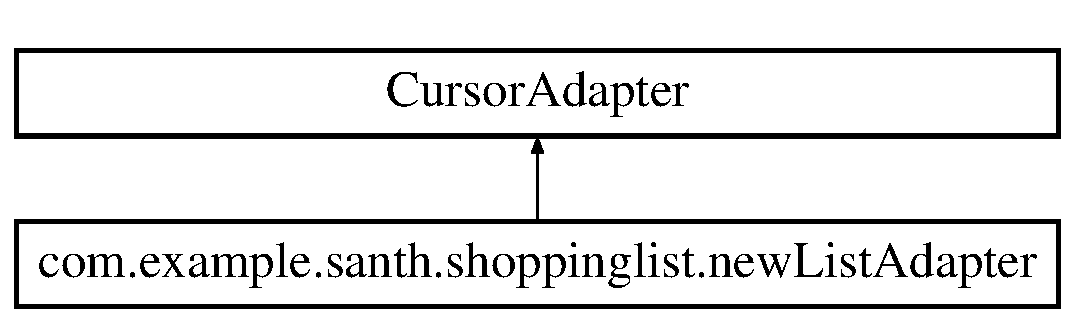
\includegraphics[height=2.000000cm]{classcom_1_1example_1_1santh_1_1shoppinglist_1_1new_list_adapter}
\end{center}
\end{figure}
\subsection*{Public Member Functions}
\begin{DoxyCompactItemize}
\item 
\hyperlink{classcom_1_1example_1_1santh_1_1shoppinglist_1_1new_list_adapter_a6588c4f209fa421cf412c9179694dfa2}{new\+List\+Adapter} (Context context, Cursor c)
\item 
View \hyperlink{classcom_1_1example_1_1santh_1_1shoppinglist_1_1new_list_adapter_aba836d3e18b7f55004be894a8bb11824}{new\+View} (final Context context, final Cursor cursor, View\+Group parent)
\begin{DoxyCompactList}\small\item\em Inflating the layout with the view. \end{DoxyCompactList}\item 
long \hyperlink{classcom_1_1example_1_1santh_1_1shoppinglist_1_1new_list_adapter_ad73c83f0b3e981b191e8ff6185d8c5a4}{get\+Item\+Id} (int pos)
\item 
void \hyperlink{classcom_1_1example_1_1santh_1_1shoppinglist_1_1new_list_adapter_a44d6e78584f2ef7351061206f467e0b3}{bind\+View} (View v, final Context context, final Cursor c)
\begin{DoxyCompactList}\small\item\em Binding the view to Layout. \end{DoxyCompactList}\end{DoxyCompactItemize}


\subsection{Detailed Description}
New\+List\+Adapter Class to Display List name and other parameters .It uses four text view Listname ,Date,List price and count of purchased items/\+Un\+Purchaseditems. 

The inflater layout has these four Text views which are binded in this adapter class 

\subsection{Constructor \& Destructor Documentation}
\index{com\+::example\+::santh\+::shoppinglist\+::new\+List\+Adapter@{com\+::example\+::santh\+::shoppinglist\+::new\+List\+Adapter}!new\+List\+Adapter@{new\+List\+Adapter}}
\index{new\+List\+Adapter@{new\+List\+Adapter}!com\+::example\+::santh\+::shoppinglist\+::new\+List\+Adapter@{com\+::example\+::santh\+::shoppinglist\+::new\+List\+Adapter}}
\subsubsection[{\texorpdfstring{new\+List\+Adapter(\+Context context, Cursor c)}{newListAdapter(Context context, Cursor c)}}]{\setlength{\rightskip}{0pt plus 5cm}com.\+example.\+santh.\+shoppinglist.\+new\+List\+Adapter.\+new\+List\+Adapter (
\begin{DoxyParamCaption}
\item[{Context}]{context, }
\item[{Cursor}]{c}
\end{DoxyParamCaption}
)}\hypertarget{classcom_1_1example_1_1santh_1_1shoppinglist_1_1new_list_adapter_a6588c4f209fa421cf412c9179694dfa2}{}\label{classcom_1_1example_1_1santh_1_1shoppinglist_1_1new_list_adapter_a6588c4f209fa421cf412c9179694dfa2}


\subsection{Member Function Documentation}
\index{com\+::example\+::santh\+::shoppinglist\+::new\+List\+Adapter@{com\+::example\+::santh\+::shoppinglist\+::new\+List\+Adapter}!bind\+View@{bind\+View}}
\index{bind\+View@{bind\+View}!com\+::example\+::santh\+::shoppinglist\+::new\+List\+Adapter@{com\+::example\+::santh\+::shoppinglist\+::new\+List\+Adapter}}
\subsubsection[{\texorpdfstring{bind\+View(\+View v, final Context context, final Cursor c)}{bindView(View v, final Context context, final Cursor c)}}]{\setlength{\rightskip}{0pt plus 5cm}void com.\+example.\+santh.\+shoppinglist.\+new\+List\+Adapter.\+bind\+View (
\begin{DoxyParamCaption}
\item[{View}]{v, }
\item[{final Context}]{context, }
\item[{final Cursor}]{c}
\end{DoxyParamCaption}
)}\hypertarget{classcom_1_1example_1_1santh_1_1shoppinglist_1_1new_list_adapter_a44d6e78584f2ef7351061206f467e0b3}{}\label{classcom_1_1example_1_1santh_1_1shoppinglist_1_1new_list_adapter_a44d6e78584f2ef7351061206f467e0b3}


Binding the view to Layout. 

\begin{DoxyAuthor}{Author}
will
\end{DoxyAuthor}

\begin{DoxyParams}{Parameters}
{\em v} & The view in which the elements we set up here will be displayed.\\
\hline
{\em context} & The running context where this List\+View adapter will be active.\\
\hline
{\em c} & The Cursor containing the query results we will display. \\
\hline
\end{DoxyParams}
\index{com\+::example\+::santh\+::shoppinglist\+::new\+List\+Adapter@{com\+::example\+::santh\+::shoppinglist\+::new\+List\+Adapter}!get\+Item\+Id@{get\+Item\+Id}}
\index{get\+Item\+Id@{get\+Item\+Id}!com\+::example\+::santh\+::shoppinglist\+::new\+List\+Adapter@{com\+::example\+::santh\+::shoppinglist\+::new\+List\+Adapter}}
\subsubsection[{\texorpdfstring{get\+Item\+Id(int pos)}{getItemId(int pos)}}]{\setlength{\rightskip}{0pt plus 5cm}long com.\+example.\+santh.\+shoppinglist.\+new\+List\+Adapter.\+get\+Item\+Id (
\begin{DoxyParamCaption}
\item[{int}]{pos}
\end{DoxyParamCaption}
)}\hypertarget{classcom_1_1example_1_1santh_1_1shoppinglist_1_1new_list_adapter_ad73c83f0b3e981b191e8ff6185d8c5a4}{}\label{classcom_1_1example_1_1santh_1_1shoppinglist_1_1new_list_adapter_ad73c83f0b3e981b191e8ff6185d8c5a4}
\index{com\+::example\+::santh\+::shoppinglist\+::new\+List\+Adapter@{com\+::example\+::santh\+::shoppinglist\+::new\+List\+Adapter}!new\+View@{new\+View}}
\index{new\+View@{new\+View}!com\+::example\+::santh\+::shoppinglist\+::new\+List\+Adapter@{com\+::example\+::santh\+::shoppinglist\+::new\+List\+Adapter}}
\subsubsection[{\texorpdfstring{new\+View(final Context context, final Cursor cursor, View\+Group parent)}{newView(final Context context, final Cursor cursor, ViewGroup parent)}}]{\setlength{\rightskip}{0pt plus 5cm}View com.\+example.\+santh.\+shoppinglist.\+new\+List\+Adapter.\+new\+View (
\begin{DoxyParamCaption}
\item[{final Context}]{context, }
\item[{final Cursor}]{cursor, }
\item[{View\+Group}]{parent}
\end{DoxyParamCaption}
)}\hypertarget{classcom_1_1example_1_1santh_1_1shoppinglist_1_1new_list_adapter_aba836d3e18b7f55004be894a8bb11824}{}\label{classcom_1_1example_1_1santh_1_1shoppinglist_1_1new_list_adapter_aba836d3e18b7f55004be894a8bb11824}


Inflating the layout with the view. 


\begin{DoxyParams}{Parameters}
{\em context} & \\
\hline
{\em cursor} & \\
\hline
{\em parent} & \\
\hline
\end{DoxyParams}
\begin{DoxyReturn}{Returns}

\end{DoxyReturn}


The documentation for this class was generated from the following file\+:\begin{DoxyCompactItemize}
\item 
E\+:/\+Android/\+Shopping\+List\+D\+B4 2/app/src/main/java/com/example/santh/shoppinglist/\hyperlink{new_list_adapter_8java}{new\+List\+Adapter.\+java}\end{DoxyCompactItemize}

\hypertarget{classcom_1_1example_1_1santh_1_1shoppinglist_1_1_settings_item_activity}{}\section{com.\+example.\+santh.\+shoppinglist.\+Settings\+Item\+Activity Class Reference}
\label{classcom_1_1example_1_1santh_1_1shoppinglist_1_1_settings_item_activity}\index{com.\+example.\+santh.\+shoppinglist.\+Settings\+Item\+Activity@{com.\+example.\+santh.\+shoppinglist.\+Settings\+Item\+Activity}}


Preference Settings for Item .Includes Sorting Items alphabetically and by category and hiding purchased items.  


Inheritance diagram for com.\+example.\+santh.\+shoppinglist.\+Settings\+Item\+Activity\+:\begin{figure}[H]
\begin{center}
\leavevmode
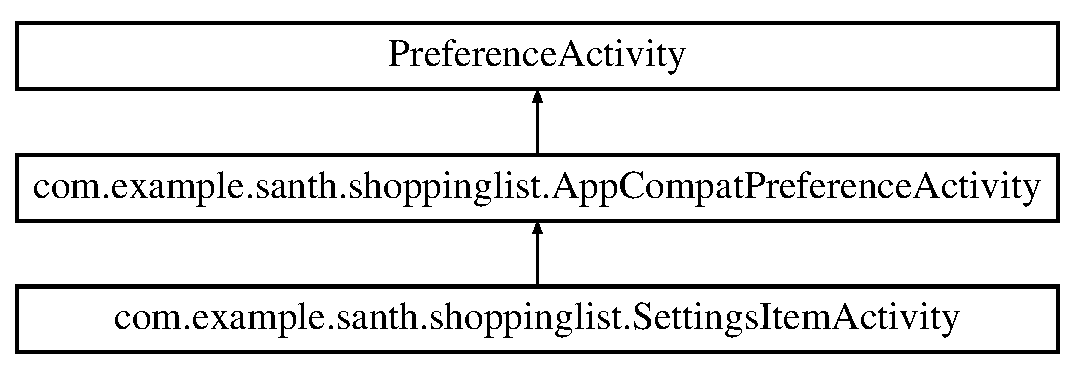
\includegraphics[height=3.000000cm]{classcom_1_1example_1_1santh_1_1shoppinglist_1_1_settings_item_activity}
\end{center}
\end{figure}
\subsection*{Classes}
\begin{DoxyCompactItemize}
\item 
class {\bfseries Settings\+Item\+Fragment}
\begin{DoxyCompactList}\small\item\em Fragement Activity class for setting preferences and generating toasts. \end{DoxyCompactList}\end{DoxyCompactItemize}
\subsection*{Public Member Functions}
\begin{DoxyCompactItemize}
\item 
void \hyperlink{classcom_1_1example_1_1santh_1_1shoppinglist_1_1_settings_item_activity_ae9dee800d9843686deafa77c06909b96}{on\+Back\+Pressed} ()
\begin{DoxyCompactList}\small\item\em on\+Back\+Pressed Method to redirect to correct intent activity \end{DoxyCompactList}\end{DoxyCompactItemize}
\subsection*{Protected Member Functions}
\begin{DoxyCompactItemize}
\item 
void \hyperlink{classcom_1_1example_1_1santh_1_1shoppinglist_1_1_settings_item_activity_ac749632b64586434c5328849272e3794}{on\+Create} (Bundle saved\+Instance\+State)
\begin{DoxyCompactList}\small\item\em A preference value change listener that updates the preference\textquotesingle{}s summary to reflect its new value. \end{DoxyCompactList}\end{DoxyCompactItemize}


\subsection{Detailed Description}
Preference Settings for Item .Includes Sorting Items alphabetically and by category and hiding purchased items. 

\subsection{Member Function Documentation}
\index{com\+::example\+::santh\+::shoppinglist\+::\+Settings\+Item\+Activity@{com\+::example\+::santh\+::shoppinglist\+::\+Settings\+Item\+Activity}!on\+Back\+Pressed@{on\+Back\+Pressed}}
\index{on\+Back\+Pressed@{on\+Back\+Pressed}!com\+::example\+::santh\+::shoppinglist\+::\+Settings\+Item\+Activity@{com\+::example\+::santh\+::shoppinglist\+::\+Settings\+Item\+Activity}}
\subsubsection[{\texorpdfstring{on\+Back\+Pressed()}{onBackPressed()}}]{\setlength{\rightskip}{0pt plus 5cm}void com.\+example.\+santh.\+shoppinglist.\+Settings\+Item\+Activity.\+on\+Back\+Pressed (
\begin{DoxyParamCaption}
{}
\end{DoxyParamCaption}
)}\hypertarget{classcom_1_1example_1_1santh_1_1shoppinglist_1_1_settings_item_activity_ae9dee800d9843686deafa77c06909b96}{}\label{classcom_1_1example_1_1santh_1_1shoppinglist_1_1_settings_item_activity_ae9dee800d9843686deafa77c06909b96}


on\+Back\+Pressed Method to redirect to correct intent activity 

\index{com\+::example\+::santh\+::shoppinglist\+::\+Settings\+Item\+Activity@{com\+::example\+::santh\+::shoppinglist\+::\+Settings\+Item\+Activity}!on\+Create@{on\+Create}}
\index{on\+Create@{on\+Create}!com\+::example\+::santh\+::shoppinglist\+::\+Settings\+Item\+Activity@{com\+::example\+::santh\+::shoppinglist\+::\+Settings\+Item\+Activity}}
\subsubsection[{\texorpdfstring{on\+Create(\+Bundle saved\+Instance\+State)}{onCreate(Bundle savedInstanceState)}}]{\setlength{\rightskip}{0pt plus 5cm}void com.\+example.\+santh.\+shoppinglist.\+Settings\+Item\+Activity.\+on\+Create (
\begin{DoxyParamCaption}
\item[{Bundle}]{saved\+Instance\+State}
\end{DoxyParamCaption}
)\hspace{0.3cm}{\ttfamily [protected]}}\hypertarget{classcom_1_1example_1_1santh_1_1shoppinglist_1_1_settings_item_activity_ac749632b64586434c5328849272e3794}{}\label{classcom_1_1example_1_1santh_1_1shoppinglist_1_1_settings_item_activity_ac749632b64586434c5328849272e3794}


A preference value change listener that updates the preference\textquotesingle{}s summary to reflect its new value. 



The documentation for this class was generated from the following file\+:\begin{DoxyCompactItemize}
\item 
E\+:/\+Android/\+Shopping\+List\+D\+B4 2/app/src/main/java/com/example/santh/shoppinglist/\hyperlink{_settings_item_activity_8java}{Settings\+Item\+Activity.\+java}\end{DoxyCompactItemize}

\hypertarget{classcom_1_1example_1_1santh_1_1shoppinglist_1_1_settings_list_activity}{}\section{com.\+example.\+santh.\+shoppinglist.\+Settings\+List\+Activity Class Reference}
\label{classcom_1_1example_1_1santh_1_1shoppinglist_1_1_settings_list_activity}\index{com.\+example.\+santh.\+shoppinglist.\+Settings\+List\+Activity@{com.\+example.\+santh.\+shoppinglist.\+Settings\+List\+Activity}}


\hyperlink{classcom_1_1example_1_1santh_1_1shoppinglist_1_1_settings_list_activity}{Settings\+List\+Activity} class for Preference settings correspoding to lists includes sorting lists by price and alphabetically .  


Inheritance diagram for com.\+example.\+santh.\+shoppinglist.\+Settings\+List\+Activity\+:\begin{figure}[H]
\begin{center}
\leavevmode
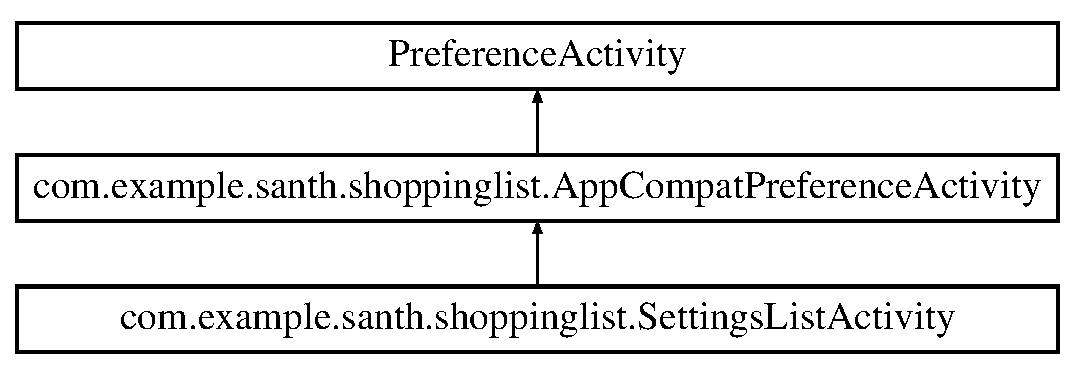
\includegraphics[height=3.000000cm]{classcom_1_1example_1_1santh_1_1shoppinglist_1_1_settings_list_activity}
\end{center}
\end{figure}
\subsection*{Classes}
\begin{DoxyCompactItemize}
\item 
class {\bfseries Settings\+List\+Fragment}
\begin{DoxyCompactList}\small\item\em Fragement Activity class for setting preferences and generating toasts. \end{DoxyCompactList}\end{DoxyCompactItemize}
\subsection*{Public Member Functions}
\begin{DoxyCompactItemize}
\item 
void \hyperlink{classcom_1_1example_1_1santh_1_1shoppinglist_1_1_settings_list_activity_a9734ce570d8bd5f31e37e12e5829e220}{on\+Back\+Pressed} ()
\begin{DoxyCompactList}\small\item\em on\+Back\+Pressed Method to redirect to correct intent activity \end{DoxyCompactList}\end{DoxyCompactItemize}
\subsection*{Protected Member Functions}
\begin{DoxyCompactItemize}
\item 
void \hyperlink{classcom_1_1example_1_1santh_1_1shoppinglist_1_1_settings_list_activity_a4d807a44c7d83866f5db353217c539ba}{on\+Create} (Bundle saved\+Instance\+State)
\begin{DoxyCompactList}\small\item\em A preference value change listener that updates the preference\textquotesingle{}s summary to reflect its new value. \end{DoxyCompactList}\end{DoxyCompactItemize}


\subsection{Detailed Description}
\hyperlink{classcom_1_1example_1_1santh_1_1shoppinglist_1_1_settings_list_activity}{Settings\+List\+Activity} class for Preference settings correspoding to lists includes sorting lists by price and alphabetically . 

And can select preffered Currency 

\subsection{Member Function Documentation}
\index{com\+::example\+::santh\+::shoppinglist\+::\+Settings\+List\+Activity@{com\+::example\+::santh\+::shoppinglist\+::\+Settings\+List\+Activity}!on\+Back\+Pressed@{on\+Back\+Pressed}}
\index{on\+Back\+Pressed@{on\+Back\+Pressed}!com\+::example\+::santh\+::shoppinglist\+::\+Settings\+List\+Activity@{com\+::example\+::santh\+::shoppinglist\+::\+Settings\+List\+Activity}}
\subsubsection[{\texorpdfstring{on\+Back\+Pressed()}{onBackPressed()}}]{\setlength{\rightskip}{0pt plus 5cm}void com.\+example.\+santh.\+shoppinglist.\+Settings\+List\+Activity.\+on\+Back\+Pressed (
\begin{DoxyParamCaption}
{}
\end{DoxyParamCaption}
)}\hypertarget{classcom_1_1example_1_1santh_1_1shoppinglist_1_1_settings_list_activity_a9734ce570d8bd5f31e37e12e5829e220}{}\label{classcom_1_1example_1_1santh_1_1shoppinglist_1_1_settings_list_activity_a9734ce570d8bd5f31e37e12e5829e220}


on\+Back\+Pressed Method to redirect to correct intent activity 

\index{com\+::example\+::santh\+::shoppinglist\+::\+Settings\+List\+Activity@{com\+::example\+::santh\+::shoppinglist\+::\+Settings\+List\+Activity}!on\+Create@{on\+Create}}
\index{on\+Create@{on\+Create}!com\+::example\+::santh\+::shoppinglist\+::\+Settings\+List\+Activity@{com\+::example\+::santh\+::shoppinglist\+::\+Settings\+List\+Activity}}
\subsubsection[{\texorpdfstring{on\+Create(\+Bundle saved\+Instance\+State)}{onCreate(Bundle savedInstanceState)}}]{\setlength{\rightskip}{0pt plus 5cm}void com.\+example.\+santh.\+shoppinglist.\+Settings\+List\+Activity.\+on\+Create (
\begin{DoxyParamCaption}
\item[{Bundle}]{saved\+Instance\+State}
\end{DoxyParamCaption}
)\hspace{0.3cm}{\ttfamily [protected]}}\hypertarget{classcom_1_1example_1_1santh_1_1shoppinglist_1_1_settings_list_activity_a4d807a44c7d83866f5db353217c539ba}{}\label{classcom_1_1example_1_1santh_1_1shoppinglist_1_1_settings_list_activity_a4d807a44c7d83866f5db353217c539ba}


A preference value change listener that updates the preference\textquotesingle{}s summary to reflect its new value. 



The documentation for this class was generated from the following file\+:\begin{DoxyCompactItemize}
\item 
E\+:/\+Android/\+Shopping\+List\+D\+B4 2/app/src/main/java/com/example/santh/shoppinglist/\hyperlink{_settings_list_activity_8java}{Settings\+List\+Activity.\+java}\end{DoxyCompactItemize}

\hypertarget{classcom_1_1example_1_1santh_1_1shoppinglist_1_1_static_data}{}\section{com.\+example.\+santh.\+shoppinglist.\+Static\+Data Class Reference}
\label{classcom_1_1example_1_1santh_1_1shoppinglist_1_1_static_data}\index{com.\+example.\+santh.\+shoppinglist.\+Static\+Data@{com.\+example.\+santh.\+shoppinglist.\+Static\+Data}}


Acessing P\+HP files using Static data Class .All Php files are accessed using this class.  


\subsection*{Public Member Functions}
\begin{DoxyCompactItemize}
\item 
int \hyperlink{classcom_1_1example_1_1santh_1_1shoppinglist_1_1_static_data_a445c4ebee6294ee8733769490e251d77}{is\+Synced} ()
\item 
void \hyperlink{classcom_1_1example_1_1santh_1_1shoppinglist_1_1_static_data_acaf2c918f21006b2327259bbe8e4c560}{reset\+Sync} ()
\item 
Networker \hyperlink{classcom_1_1example_1_1santh_1_1shoppinglist_1_1_static_data_a3fa6524314249be47286f9c1e77fcd38}{Sync\+With\+External} (String link)
\begin{DoxyCompactList}\small\item\em Makes and runs a Networker Thread using some link. \end{DoxyCompactList}\end{DoxyCompactItemize}
\subsection*{Static Public Member Functions}
\begin{DoxyCompactItemize}
\item 
static \hyperlink{classcom_1_1example_1_1santh_1_1shoppinglist_1_1_static_data}{Static\+Data} \hyperlink{classcom_1_1example_1_1santh_1_1shoppinglist_1_1_static_data_aa8186e28e5e45b71c96b252fe5b95e7a}{get\+Instance} ()
\end{DoxyCompactItemize}
\subsection*{Public Attributes}
\begin{DoxyCompactItemize}
\item 
J\+S\+O\+N\+Array \hyperlink{classcom_1_1example_1_1santh_1_1shoppinglist_1_1_static_data_a2e553853981a2db0df178ecaa73b3a6a}{lists}
\item 
J\+S\+O\+N\+Array \hyperlink{classcom_1_1example_1_1santh_1_1shoppinglist_1_1_static_data_a8396eedfbdf79abf82f0081dc135af42}{Items}
\item 
J\+S\+O\+N\+Array \hyperlink{classcom_1_1example_1_1santh_1_1shoppinglist_1_1_static_data_a44bfa240d7ced9aa65e395d1f37e32c0}{units}
\item 
J\+S\+O\+N\+Array \hyperlink{classcom_1_1example_1_1santh_1_1shoppinglist_1_1_static_data_af1a56c4d85d465ddfbd3ffcd5d3c35a6}{catgeories}
\item 
J\+S\+O\+N\+Array \hyperlink{classcom_1_1example_1_1santh_1_1shoppinglist_1_1_static_data_a1d8214e43fc91fea8431ea2caea3b64f}{deleteid}
\item 
J\+S\+O\+N\+Array \hyperlink{classcom_1_1example_1_1santh_1_1shoppinglist_1_1_static_data_ad458aa6dd2d751e4cb6e393332cf753d}{deleteunit}
\item 
J\+S\+O\+N\+Array \hyperlink{classcom_1_1example_1_1santh_1_1shoppinglist_1_1_static_data_aaa46e350a44590604f7ef9057e1b6e55}{deeletecategory}
\item 
String \hyperlink{classcom_1_1example_1_1santh_1_1shoppinglist_1_1_static_data_ab79e46d3d064f42471fa34c85f69e81b}{update\+Time}
\end{DoxyCompactItemize}
\subsection*{Static Public Attributes}
\begin{DoxyCompactItemize}
\item 
static final String \hyperlink{classcom_1_1example_1_1santh_1_1shoppinglist_1_1_static_data_a92d144da22eec752791d44cee54099f4}{get\+Lists} = view\+P\+HP + \char`\"{}db\+\_\+getalllists.\+php\char`\"{}
\item 
static final String \hyperlink{classcom_1_1example_1_1santh_1_1shoppinglist_1_1_static_data_afd0845d4cf7cebc48b5bfa68b37e6b1a}{get\+Items} = view\+P\+HP + \char`\"{}db\+\_\+getallitems.\+php\char`\"{}
\item 
static final String \hyperlink{classcom_1_1example_1_1santh_1_1shoppinglist_1_1_static_data_a4ef15e32e18002772a06d568342642c7}{get\+Units} = view\+P\+HP + \char`\"{}db\+\_\+getallunits.\+php\char`\"{}
\item 
static final String \hyperlink{classcom_1_1example_1_1santh_1_1shoppinglist_1_1_static_data_a6526d7f1092c447e40d19b21f0dd2878}{get\+Categories} = view\+P\+HP + \char`\"{}db\+\_\+getallcategories.\+php\char`\"{}
\item 
static final String \hyperlink{classcom_1_1example_1_1santh_1_1shoppinglist_1_1_static_data_ac1c3487b59fa7dc543056e03103f9858}{getdeletelist} =\char`\"{}http\+://people.\+cs.\+clemson.\+edu/$\sim$sravira/Delete/db\+\_\+getdeletelist.\+php\char`\"{}
\item 
static final String \hyperlink{classcom_1_1example_1_1santh_1_1shoppinglist_1_1_static_data_ada7d599d828b29d17bcbfc8764d2f53a}{getdeleteunit} =\char`\"{}http\+://people.\+cs.\+clemson.\+edu/$\sim$sravira/Delete/db\+\_\+getdeleteunit.\+php\char`\"{}
\item 
static final String \hyperlink{classcom_1_1example_1_1santh_1_1shoppinglist_1_1_static_data_a1f83fd9c57993c3a15c4329b8b5eafc6}{getdeletecategory} =\char`\"{}http\+://people.\+cs.\+clemson.\+edu/$\sim$sravira/Delete/db\+\_\+getdeletecategory.\+php\char`\"{}
\end{DoxyCompactItemize}


\subsection{Detailed Description}
Acessing P\+HP files using Static data Class .All Php files are accessed using this class. 

\subsection{Member Function Documentation}
\index{com\+::example\+::santh\+::shoppinglist\+::\+Static\+Data@{com\+::example\+::santh\+::shoppinglist\+::\+Static\+Data}!get\+Instance@{get\+Instance}}
\index{get\+Instance@{get\+Instance}!com\+::example\+::santh\+::shoppinglist\+::\+Static\+Data@{com\+::example\+::santh\+::shoppinglist\+::\+Static\+Data}}
\subsubsection[{\texorpdfstring{get\+Instance()}{getInstance()}}]{\setlength{\rightskip}{0pt plus 5cm}static {\bf Static\+Data} com.\+example.\+santh.\+shoppinglist.\+Static\+Data.\+get\+Instance (
\begin{DoxyParamCaption}
{}
\end{DoxyParamCaption}
)\hspace{0.3cm}{\ttfamily [static]}}\hypertarget{classcom_1_1example_1_1santh_1_1shoppinglist_1_1_static_data_aa8186e28e5e45b71c96b252fe5b95e7a}{}\label{classcom_1_1example_1_1santh_1_1shoppinglist_1_1_static_data_aa8186e28e5e45b71c96b252fe5b95e7a}
\index{com\+::example\+::santh\+::shoppinglist\+::\+Static\+Data@{com\+::example\+::santh\+::shoppinglist\+::\+Static\+Data}!is\+Synced@{is\+Synced}}
\index{is\+Synced@{is\+Synced}!com\+::example\+::santh\+::shoppinglist\+::\+Static\+Data@{com\+::example\+::santh\+::shoppinglist\+::\+Static\+Data}}
\subsubsection[{\texorpdfstring{is\+Synced()}{isSynced()}}]{\setlength{\rightskip}{0pt plus 5cm}int com.\+example.\+santh.\+shoppinglist.\+Static\+Data.\+is\+Synced (
\begin{DoxyParamCaption}
{}
\end{DoxyParamCaption}
)}\hypertarget{classcom_1_1example_1_1santh_1_1shoppinglist_1_1_static_data_a445c4ebee6294ee8733769490e251d77}{}\label{classcom_1_1example_1_1santh_1_1shoppinglist_1_1_static_data_a445c4ebee6294ee8733769490e251d77}
\index{com\+::example\+::santh\+::shoppinglist\+::\+Static\+Data@{com\+::example\+::santh\+::shoppinglist\+::\+Static\+Data}!reset\+Sync@{reset\+Sync}}
\index{reset\+Sync@{reset\+Sync}!com\+::example\+::santh\+::shoppinglist\+::\+Static\+Data@{com\+::example\+::santh\+::shoppinglist\+::\+Static\+Data}}
\subsubsection[{\texorpdfstring{reset\+Sync()}{resetSync()}}]{\setlength{\rightskip}{0pt plus 5cm}void com.\+example.\+santh.\+shoppinglist.\+Static\+Data.\+reset\+Sync (
\begin{DoxyParamCaption}
{}
\end{DoxyParamCaption}
)}\hypertarget{classcom_1_1example_1_1santh_1_1shoppinglist_1_1_static_data_acaf2c918f21006b2327259bbe8e4c560}{}\label{classcom_1_1example_1_1santh_1_1shoppinglist_1_1_static_data_acaf2c918f21006b2327259bbe8e4c560}
\index{com\+::example\+::santh\+::shoppinglist\+::\+Static\+Data@{com\+::example\+::santh\+::shoppinglist\+::\+Static\+Data}!Sync\+With\+External@{Sync\+With\+External}}
\index{Sync\+With\+External@{Sync\+With\+External}!com\+::example\+::santh\+::shoppinglist\+::\+Static\+Data@{com\+::example\+::santh\+::shoppinglist\+::\+Static\+Data}}
\subsubsection[{\texorpdfstring{Sync\+With\+External(\+String link)}{SyncWithExternal(String link)}}]{\setlength{\rightskip}{0pt plus 5cm}Networker com.\+example.\+santh.\+shoppinglist.\+Static\+Data.\+Sync\+With\+External (
\begin{DoxyParamCaption}
\item[{String}]{link}
\end{DoxyParamCaption}
)}\hypertarget{classcom_1_1example_1_1santh_1_1shoppinglist_1_1_static_data_a3fa6524314249be47286f9c1e77fcd38}{}\label{classcom_1_1example_1_1santh_1_1shoppinglist_1_1_static_data_a3fa6524314249be47286f9c1e77fcd38}


Makes and runs a Networker Thread using some link. 



\subsection{Member Data Documentation}
\index{com\+::example\+::santh\+::shoppinglist\+::\+Static\+Data@{com\+::example\+::santh\+::shoppinglist\+::\+Static\+Data}!catgeories@{catgeories}}
\index{catgeories@{catgeories}!com\+::example\+::santh\+::shoppinglist\+::\+Static\+Data@{com\+::example\+::santh\+::shoppinglist\+::\+Static\+Data}}
\subsubsection[{\texorpdfstring{catgeories}{catgeories}}]{\setlength{\rightskip}{0pt plus 5cm}J\+S\+O\+N\+Array com.\+example.\+santh.\+shoppinglist.\+Static\+Data.\+catgeories}\hypertarget{classcom_1_1example_1_1santh_1_1shoppinglist_1_1_static_data_af1a56c4d85d465ddfbd3ffcd5d3c35a6}{}\label{classcom_1_1example_1_1santh_1_1shoppinglist_1_1_static_data_af1a56c4d85d465ddfbd3ffcd5d3c35a6}
\index{com\+::example\+::santh\+::shoppinglist\+::\+Static\+Data@{com\+::example\+::santh\+::shoppinglist\+::\+Static\+Data}!deeletecategory@{deeletecategory}}
\index{deeletecategory@{deeletecategory}!com\+::example\+::santh\+::shoppinglist\+::\+Static\+Data@{com\+::example\+::santh\+::shoppinglist\+::\+Static\+Data}}
\subsubsection[{\texorpdfstring{deeletecategory}{deeletecategory}}]{\setlength{\rightskip}{0pt plus 5cm}J\+S\+O\+N\+Array com.\+example.\+santh.\+shoppinglist.\+Static\+Data.\+deeletecategory}\hypertarget{classcom_1_1example_1_1santh_1_1shoppinglist_1_1_static_data_aaa46e350a44590604f7ef9057e1b6e55}{}\label{classcom_1_1example_1_1santh_1_1shoppinglist_1_1_static_data_aaa46e350a44590604f7ef9057e1b6e55}
\index{com\+::example\+::santh\+::shoppinglist\+::\+Static\+Data@{com\+::example\+::santh\+::shoppinglist\+::\+Static\+Data}!deleteid@{deleteid}}
\index{deleteid@{deleteid}!com\+::example\+::santh\+::shoppinglist\+::\+Static\+Data@{com\+::example\+::santh\+::shoppinglist\+::\+Static\+Data}}
\subsubsection[{\texorpdfstring{deleteid}{deleteid}}]{\setlength{\rightskip}{0pt plus 5cm}J\+S\+O\+N\+Array com.\+example.\+santh.\+shoppinglist.\+Static\+Data.\+deleteid}\hypertarget{classcom_1_1example_1_1santh_1_1shoppinglist_1_1_static_data_a1d8214e43fc91fea8431ea2caea3b64f}{}\label{classcom_1_1example_1_1santh_1_1shoppinglist_1_1_static_data_a1d8214e43fc91fea8431ea2caea3b64f}
\index{com\+::example\+::santh\+::shoppinglist\+::\+Static\+Data@{com\+::example\+::santh\+::shoppinglist\+::\+Static\+Data}!deleteunit@{deleteunit}}
\index{deleteunit@{deleteunit}!com\+::example\+::santh\+::shoppinglist\+::\+Static\+Data@{com\+::example\+::santh\+::shoppinglist\+::\+Static\+Data}}
\subsubsection[{\texorpdfstring{deleteunit}{deleteunit}}]{\setlength{\rightskip}{0pt plus 5cm}J\+S\+O\+N\+Array com.\+example.\+santh.\+shoppinglist.\+Static\+Data.\+deleteunit}\hypertarget{classcom_1_1example_1_1santh_1_1shoppinglist_1_1_static_data_ad458aa6dd2d751e4cb6e393332cf753d}{}\label{classcom_1_1example_1_1santh_1_1shoppinglist_1_1_static_data_ad458aa6dd2d751e4cb6e393332cf753d}
\index{com\+::example\+::santh\+::shoppinglist\+::\+Static\+Data@{com\+::example\+::santh\+::shoppinglist\+::\+Static\+Data}!get\+Categories@{get\+Categories}}
\index{get\+Categories@{get\+Categories}!com\+::example\+::santh\+::shoppinglist\+::\+Static\+Data@{com\+::example\+::santh\+::shoppinglist\+::\+Static\+Data}}
\subsubsection[{\texorpdfstring{get\+Categories}{getCategories}}]{\setlength{\rightskip}{0pt plus 5cm}final String com.\+example.\+santh.\+shoppinglist.\+Static\+Data.\+get\+Categories = view\+P\+HP + \char`\"{}db\+\_\+getallcategories.\+php\char`\"{}\hspace{0.3cm}{\ttfamily [static]}}\hypertarget{classcom_1_1example_1_1santh_1_1shoppinglist_1_1_static_data_a6526d7f1092c447e40d19b21f0dd2878}{}\label{classcom_1_1example_1_1santh_1_1shoppinglist_1_1_static_data_a6526d7f1092c447e40d19b21f0dd2878}
\index{com\+::example\+::santh\+::shoppinglist\+::\+Static\+Data@{com\+::example\+::santh\+::shoppinglist\+::\+Static\+Data}!getdeletecategory@{getdeletecategory}}
\index{getdeletecategory@{getdeletecategory}!com\+::example\+::santh\+::shoppinglist\+::\+Static\+Data@{com\+::example\+::santh\+::shoppinglist\+::\+Static\+Data}}
\subsubsection[{\texorpdfstring{getdeletecategory}{getdeletecategory}}]{\setlength{\rightskip}{0pt plus 5cm}final String com.\+example.\+santh.\+shoppinglist.\+Static\+Data.\+getdeletecategory =\char`\"{}http\+://people.\+cs.\+clemson.\+edu/$\sim$sravira/Delete/db\+\_\+getdeletecategory.\+php\char`\"{}\hspace{0.3cm}{\ttfamily [static]}}\hypertarget{classcom_1_1example_1_1santh_1_1shoppinglist_1_1_static_data_a1f83fd9c57993c3a15c4329b8b5eafc6}{}\label{classcom_1_1example_1_1santh_1_1shoppinglist_1_1_static_data_a1f83fd9c57993c3a15c4329b8b5eafc6}
\index{com\+::example\+::santh\+::shoppinglist\+::\+Static\+Data@{com\+::example\+::santh\+::shoppinglist\+::\+Static\+Data}!getdeletelist@{getdeletelist}}
\index{getdeletelist@{getdeletelist}!com\+::example\+::santh\+::shoppinglist\+::\+Static\+Data@{com\+::example\+::santh\+::shoppinglist\+::\+Static\+Data}}
\subsubsection[{\texorpdfstring{getdeletelist}{getdeletelist}}]{\setlength{\rightskip}{0pt plus 5cm}final String com.\+example.\+santh.\+shoppinglist.\+Static\+Data.\+getdeletelist =\char`\"{}http\+://people.\+cs.\+clemson.\+edu/$\sim$sravira/Delete/db\+\_\+getdeletelist.\+php\char`\"{}\hspace{0.3cm}{\ttfamily [static]}}\hypertarget{classcom_1_1example_1_1santh_1_1shoppinglist_1_1_static_data_ac1c3487b59fa7dc543056e03103f9858}{}\label{classcom_1_1example_1_1santh_1_1shoppinglist_1_1_static_data_ac1c3487b59fa7dc543056e03103f9858}
\index{com\+::example\+::santh\+::shoppinglist\+::\+Static\+Data@{com\+::example\+::santh\+::shoppinglist\+::\+Static\+Data}!getdeleteunit@{getdeleteunit}}
\index{getdeleteunit@{getdeleteunit}!com\+::example\+::santh\+::shoppinglist\+::\+Static\+Data@{com\+::example\+::santh\+::shoppinglist\+::\+Static\+Data}}
\subsubsection[{\texorpdfstring{getdeleteunit}{getdeleteunit}}]{\setlength{\rightskip}{0pt plus 5cm}final String com.\+example.\+santh.\+shoppinglist.\+Static\+Data.\+getdeleteunit =\char`\"{}http\+://people.\+cs.\+clemson.\+edu/$\sim$sravira/Delete/db\+\_\+getdeleteunit.\+php\char`\"{}\hspace{0.3cm}{\ttfamily [static]}}\hypertarget{classcom_1_1example_1_1santh_1_1shoppinglist_1_1_static_data_ada7d599d828b29d17bcbfc8764d2f53a}{}\label{classcom_1_1example_1_1santh_1_1shoppinglist_1_1_static_data_ada7d599d828b29d17bcbfc8764d2f53a}
\index{com\+::example\+::santh\+::shoppinglist\+::\+Static\+Data@{com\+::example\+::santh\+::shoppinglist\+::\+Static\+Data}!get\+Items@{get\+Items}}
\index{get\+Items@{get\+Items}!com\+::example\+::santh\+::shoppinglist\+::\+Static\+Data@{com\+::example\+::santh\+::shoppinglist\+::\+Static\+Data}}
\subsubsection[{\texorpdfstring{get\+Items}{getItems}}]{\setlength{\rightskip}{0pt plus 5cm}final String com.\+example.\+santh.\+shoppinglist.\+Static\+Data.\+get\+Items = view\+P\+HP + \char`\"{}db\+\_\+getallitems.\+php\char`\"{}\hspace{0.3cm}{\ttfamily [static]}}\hypertarget{classcom_1_1example_1_1santh_1_1shoppinglist_1_1_static_data_afd0845d4cf7cebc48b5bfa68b37e6b1a}{}\label{classcom_1_1example_1_1santh_1_1shoppinglist_1_1_static_data_afd0845d4cf7cebc48b5bfa68b37e6b1a}
\index{com\+::example\+::santh\+::shoppinglist\+::\+Static\+Data@{com\+::example\+::santh\+::shoppinglist\+::\+Static\+Data}!get\+Lists@{get\+Lists}}
\index{get\+Lists@{get\+Lists}!com\+::example\+::santh\+::shoppinglist\+::\+Static\+Data@{com\+::example\+::santh\+::shoppinglist\+::\+Static\+Data}}
\subsubsection[{\texorpdfstring{get\+Lists}{getLists}}]{\setlength{\rightskip}{0pt plus 5cm}final String com.\+example.\+santh.\+shoppinglist.\+Static\+Data.\+get\+Lists = view\+P\+HP + \char`\"{}db\+\_\+getalllists.\+php\char`\"{}\hspace{0.3cm}{\ttfamily [static]}}\hypertarget{classcom_1_1example_1_1santh_1_1shoppinglist_1_1_static_data_a92d144da22eec752791d44cee54099f4}{}\label{classcom_1_1example_1_1santh_1_1shoppinglist_1_1_static_data_a92d144da22eec752791d44cee54099f4}
\index{com\+::example\+::santh\+::shoppinglist\+::\+Static\+Data@{com\+::example\+::santh\+::shoppinglist\+::\+Static\+Data}!get\+Units@{get\+Units}}
\index{get\+Units@{get\+Units}!com\+::example\+::santh\+::shoppinglist\+::\+Static\+Data@{com\+::example\+::santh\+::shoppinglist\+::\+Static\+Data}}
\subsubsection[{\texorpdfstring{get\+Units}{getUnits}}]{\setlength{\rightskip}{0pt plus 5cm}final String com.\+example.\+santh.\+shoppinglist.\+Static\+Data.\+get\+Units = view\+P\+HP + \char`\"{}db\+\_\+getallunits.\+php\char`\"{}\hspace{0.3cm}{\ttfamily [static]}}\hypertarget{classcom_1_1example_1_1santh_1_1shoppinglist_1_1_static_data_a4ef15e32e18002772a06d568342642c7}{}\label{classcom_1_1example_1_1santh_1_1shoppinglist_1_1_static_data_a4ef15e32e18002772a06d568342642c7}
\index{com\+::example\+::santh\+::shoppinglist\+::\+Static\+Data@{com\+::example\+::santh\+::shoppinglist\+::\+Static\+Data}!Items@{Items}}
\index{Items@{Items}!com\+::example\+::santh\+::shoppinglist\+::\+Static\+Data@{com\+::example\+::santh\+::shoppinglist\+::\+Static\+Data}}
\subsubsection[{\texorpdfstring{Items}{Items}}]{\setlength{\rightskip}{0pt plus 5cm}J\+S\+O\+N\+Array com.\+example.\+santh.\+shoppinglist.\+Static\+Data.\+Items}\hypertarget{classcom_1_1example_1_1santh_1_1shoppinglist_1_1_static_data_a8396eedfbdf79abf82f0081dc135af42}{}\label{classcom_1_1example_1_1santh_1_1shoppinglist_1_1_static_data_a8396eedfbdf79abf82f0081dc135af42}
\index{com\+::example\+::santh\+::shoppinglist\+::\+Static\+Data@{com\+::example\+::santh\+::shoppinglist\+::\+Static\+Data}!lists@{lists}}
\index{lists@{lists}!com\+::example\+::santh\+::shoppinglist\+::\+Static\+Data@{com\+::example\+::santh\+::shoppinglist\+::\+Static\+Data}}
\subsubsection[{\texorpdfstring{lists}{lists}}]{\setlength{\rightskip}{0pt plus 5cm}J\+S\+O\+N\+Array com.\+example.\+santh.\+shoppinglist.\+Static\+Data.\+lists}\hypertarget{classcom_1_1example_1_1santh_1_1shoppinglist_1_1_static_data_a2e553853981a2db0df178ecaa73b3a6a}{}\label{classcom_1_1example_1_1santh_1_1shoppinglist_1_1_static_data_a2e553853981a2db0df178ecaa73b3a6a}
\index{com\+::example\+::santh\+::shoppinglist\+::\+Static\+Data@{com\+::example\+::santh\+::shoppinglist\+::\+Static\+Data}!units@{units}}
\index{units@{units}!com\+::example\+::santh\+::shoppinglist\+::\+Static\+Data@{com\+::example\+::santh\+::shoppinglist\+::\+Static\+Data}}
\subsubsection[{\texorpdfstring{units}{units}}]{\setlength{\rightskip}{0pt plus 5cm}J\+S\+O\+N\+Array com.\+example.\+santh.\+shoppinglist.\+Static\+Data.\+units}\hypertarget{classcom_1_1example_1_1santh_1_1shoppinglist_1_1_static_data_a44bfa240d7ced9aa65e395d1f37e32c0}{}\label{classcom_1_1example_1_1santh_1_1shoppinglist_1_1_static_data_a44bfa240d7ced9aa65e395d1f37e32c0}
\index{com\+::example\+::santh\+::shoppinglist\+::\+Static\+Data@{com\+::example\+::santh\+::shoppinglist\+::\+Static\+Data}!update\+Time@{update\+Time}}
\index{update\+Time@{update\+Time}!com\+::example\+::santh\+::shoppinglist\+::\+Static\+Data@{com\+::example\+::santh\+::shoppinglist\+::\+Static\+Data}}
\subsubsection[{\texorpdfstring{update\+Time}{updateTime}}]{\setlength{\rightskip}{0pt plus 5cm}String com.\+example.\+santh.\+shoppinglist.\+Static\+Data.\+update\+Time}\hypertarget{classcom_1_1example_1_1santh_1_1shoppinglist_1_1_static_data_ab79e46d3d064f42471fa34c85f69e81b}{}\label{classcom_1_1example_1_1santh_1_1shoppinglist_1_1_static_data_ab79e46d3d064f42471fa34c85f69e81b}


The documentation for this class was generated from the following file\+:\begin{DoxyCompactItemize}
\item 
E\+:/\+Android/\+Shopping\+List\+D\+B4 2/app/src/main/java/com/example/santh/shoppinglist/\hyperlink{_static_data_8java}{Static\+Data.\+java}\end{DoxyCompactItemize}

\chapter{File Documentation}
\hypertarget{_app_compat_preference_activity_8java}{}\section{E\+:/\+Android/\+Shopping\+List\+D\+B4 2/app/src/main/java/com/example/santh/shoppinglist/\+App\+Compat\+Preference\+Activity.java File Reference}
\label{_app_compat_preference_activity_8java}\index{E\+:/\+Android/\+Shopping\+List\+D\+B4 2/app/src/main/java/com/example/santh/shoppinglist/\+App\+Compat\+Preference\+Activity.\+java@{E\+:/\+Android/\+Shopping\+List\+D\+B4 2/app/src/main/java/com/example/santh/shoppinglist/\+App\+Compat\+Preference\+Activity.\+java}}
\subsection*{Classes}
\begin{DoxyCompactItemize}
\item 
class \hyperlink{classcom_1_1example_1_1santh_1_1shoppinglist_1_1_app_compat_preference_activity}{com.\+example.\+santh.\+shoppinglist.\+App\+Compat\+Preference\+Activity}
\begin{DoxyCompactList}\small\item\em A \hyperlink{}{android.\+preference.\+Preference\+Activity} which implements and proxies the necessary calls to be used with App\+Compat. \end{DoxyCompactList}\end{DoxyCompactItemize}
\subsection*{Packages}
\begin{DoxyCompactItemize}
\item 
package \hyperlink{namespacecom_1_1example_1_1santh_1_1shoppinglist}{com.\+example.\+santh.\+shoppinglist}
\end{DoxyCompactItemize}

\hypertarget{_custom_auto_complete_text_changed_listener_8java}{}\section{E\+:/\+Android/\+Shopping\+List\+D\+B4 2/app/src/main/java/com/example/santh/shoppinglist/\+Custom\+Auto\+Complete\+Text\+Changed\+Listener.java File Reference}
\label{_custom_auto_complete_text_changed_listener_8java}\index{E\+:/\+Android/\+Shopping\+List\+D\+B4 2/app/src/main/java/com/example/santh/shoppinglist/\+Custom\+Auto\+Complete\+Text\+Changed\+Listener.\+java@{E\+:/\+Android/\+Shopping\+List\+D\+B4 2/app/src/main/java/com/example/santh/shoppinglist/\+Custom\+Auto\+Complete\+Text\+Changed\+Listener.\+java}}
\subsection*{Classes}
\begin{DoxyCompactItemize}
\item 
class \hyperlink{classcom_1_1example_1_1santh_1_1shoppinglist_1_1_custom_auto_complete_text_changed_listener}{com.\+example.\+santh.\+shoppinglist.\+Custom\+Auto\+Complete\+Text\+Changed\+Listener}
\begin{DoxyCompactList}\small\item\em \hyperlink{classcom_1_1example_1_1santh_1_1shoppinglist_1_1_custom_auto_complete_text_changed_listener}{Custom\+Auto\+Complete\+Text\+Changed\+Listener} is used to get the Products from DB when a character has been changed by user. \end{DoxyCompactList}\end{DoxyCompactItemize}
\subsection*{Packages}
\begin{DoxyCompactItemize}
\item 
package \hyperlink{namespacecom_1_1example_1_1santh_1_1shoppinglist}{com.\+example.\+santh.\+shoppinglist}
\end{DoxyCompactItemize}

\hypertarget{_custom_auto_complete_view_8java}{}\section{E\+:/\+Android/\+Shopping\+List\+D\+B4 2/app/src/main/java/com/example/santh/shoppinglist/\+Custom\+Auto\+Complete\+View.java File Reference}
\label{_custom_auto_complete_view_8java}\index{E\+:/\+Android/\+Shopping\+List\+D\+B4 2/app/src/main/java/com/example/santh/shoppinglist/\+Custom\+Auto\+Complete\+View.\+java@{E\+:/\+Android/\+Shopping\+List\+D\+B4 2/app/src/main/java/com/example/santh/shoppinglist/\+Custom\+Auto\+Complete\+View.\+java}}
\subsection*{Classes}
\begin{DoxyCompactItemize}
\item 
class \hyperlink{classcom_1_1example_1_1santh_1_1shoppinglist_1_1_custom_auto_complete_view}{com.\+example.\+santh.\+shoppinglist.\+Custom\+Auto\+Complete\+View}
\begin{DoxyCompactList}\small\item\em Cutsom\+Auto\+Complete\+View takes the text entered in the field and shows the matching products suggestions to users. \end{DoxyCompactList}\end{DoxyCompactItemize}
\subsection*{Packages}
\begin{DoxyCompactItemize}
\item 
package \hyperlink{namespacecom_1_1example_1_1santh_1_1shoppinglist}{com.\+example.\+santh.\+shoppinglist}
\end{DoxyCompactItemize}

\hypertarget{_data_base_manager_8java}{}\section{E\+:/\+Android/\+Shopping\+List\+D\+B4 2/app/src/main/java/com/example/santh/shoppinglist/\+Data\+Base\+Manager.java File Reference}
\label{_data_base_manager_8java}\index{E\+:/\+Android/\+Shopping\+List\+D\+B4 2/app/src/main/java/com/example/santh/shoppinglist/\+Data\+Base\+Manager.\+java@{E\+:/\+Android/\+Shopping\+List\+D\+B4 2/app/src/main/java/com/example/santh/shoppinglist/\+Data\+Base\+Manager.\+java}}
\subsection*{Classes}
\begin{DoxyCompactItemize}
\item 
class \hyperlink{classcom_1_1example_1_1santh_1_1shoppinglist_1_1_data_base_manager}{com.\+example.\+santh.\+shoppinglist.\+Data\+Base\+Manager}
\begin{DoxyCompactList}\small\item\em \hyperlink{classcom_1_1example_1_1santh_1_1shoppinglist_1_1_data_base_manager}{Data\+Base\+Manager} class file to edit delete update and query the database. \end{DoxyCompactList}\end{DoxyCompactItemize}
\subsection*{Packages}
\begin{DoxyCompactItemize}
\item 
package \hyperlink{namespacecom_1_1example_1_1santh_1_1shoppinglist}{com.\+example.\+santh.\+shoppinglist}
\end{DoxyCompactItemize}

\hypertarget{_info_activity_8java}{}\section{E\+:/\+Android/\+Shopping\+List\+D\+B4 2/app/src/main/java/com/example/santh/shoppinglist/\+Info\+Activity.java File Reference}
\label{_info_activity_8java}\index{E\+:/\+Android/\+Shopping\+List\+D\+B4 2/app/src/main/java/com/example/santh/shoppinglist/\+Info\+Activity.\+java@{E\+:/\+Android/\+Shopping\+List\+D\+B4 2/app/src/main/java/com/example/santh/shoppinglist/\+Info\+Activity.\+java}}
\subsection*{Classes}
\begin{DoxyCompactItemize}
\item 
class \hyperlink{classcom_1_1example_1_1santh_1_1shoppinglist_1_1_info_activity}{com.\+example.\+santh.\+shoppinglist.\+Info\+Activity}
\begin{DoxyCompactList}\small\item\em Info Activity Class for description of App. \end{DoxyCompactList}\end{DoxyCompactItemize}
\subsection*{Packages}
\begin{DoxyCompactItemize}
\item 
package \hyperlink{namespacecom_1_1example_1_1santh_1_1shoppinglist}{com.\+example.\+santh.\+shoppinglist}
\end{DoxyCompactItemize}

\hypertarget{_item_activity_8java}{}\section{E\+:/\+Android/\+Shopping\+List\+D\+B4 2/app/src/main/java/com/example/santh/shoppinglist/\+Item\+Activity.java File Reference}
\label{_item_activity_8java}\index{E\+:/\+Android/\+Shopping\+List\+D\+B4 2/app/src/main/java/com/example/santh/shoppinglist/\+Item\+Activity.\+java@{E\+:/\+Android/\+Shopping\+List\+D\+B4 2/app/src/main/java/com/example/santh/shoppinglist/\+Item\+Activity.\+java}}
\subsection*{Classes}
\begin{DoxyCompactItemize}
\item 
class \hyperlink{classcom_1_1example_1_1santh_1_1shoppinglist_1_1_item_activity}{com.\+example.\+santh.\+shoppinglist.\+Item\+Activity}
\begin{DoxyCompactList}\small\item\em This is a Item class which is used to add an item to list .Update the item. \end{DoxyCompactList}\item 
class {\bfseries com.\+example.\+santh.\+shoppinglist.\+Item\+Activity.\+Roll}
\end{DoxyCompactItemize}
\subsection*{Packages}
\begin{DoxyCompactItemize}
\item 
package \hyperlink{namespacecom_1_1example_1_1santh_1_1shoppinglist}{com.\+example.\+santh.\+shoppinglist}
\end{DoxyCompactItemize}

\hypertarget{_j_s_o_n_parser_8java}{}\section{E\+:/\+Android/\+Shopping\+List\+D\+B4 2/app/src/main/java/com/example/santh/shoppinglist/\+J\+S\+O\+N\+Parser.java File Reference}
\label{_j_s_o_n_parser_8java}\index{E\+:/\+Android/\+Shopping\+List\+D\+B4 2/app/src/main/java/com/example/santh/shoppinglist/\+J\+S\+O\+N\+Parser.\+java@{E\+:/\+Android/\+Shopping\+List\+D\+B4 2/app/src/main/java/com/example/santh/shoppinglist/\+J\+S\+O\+N\+Parser.\+java}}
\subsection*{Classes}
\begin{DoxyCompactItemize}
\item 
class \hyperlink{classcom_1_1example_1_1santh_1_1shoppinglist_1_1_j_s_o_n_parser}{com.\+example.\+santh.\+shoppinglist.\+J\+S\+O\+N\+Parser}
\begin{DoxyCompactList}\small\item\em J\+S\+ON Parser class to convert entries into J\+S\+ON array. \end{DoxyCompactList}\end{DoxyCompactItemize}
\subsection*{Packages}
\begin{DoxyCompactItemize}
\item 
package \hyperlink{namespacecom_1_1example_1_1santh_1_1shoppinglist}{com.\+example.\+santh.\+shoppinglist}
\end{DoxyCompactItemize}

\hypertarget{_launch_activity_8java}{}\section{E\+:/\+Android/\+Shopping\+List\+D\+B4 2/app/src/main/java/com/example/santh/shoppinglist/\+Launch\+Activity.java File Reference}
\label{_launch_activity_8java}\index{E\+:/\+Android/\+Shopping\+List\+D\+B4 2/app/src/main/java/com/example/santh/shoppinglist/\+Launch\+Activity.\+java@{E\+:/\+Android/\+Shopping\+List\+D\+B4 2/app/src/main/java/com/example/santh/shoppinglist/\+Launch\+Activity.\+java}}
\subsection*{Classes}
\begin{DoxyCompactItemize}
\item 
class \hyperlink{classcom_1_1example_1_1santh_1_1shoppinglist_1_1_launch_activity}{com.\+example.\+santh.\+shoppinglist.\+Launch\+Activity}
\begin{DoxyCompactList}\small\item\em \hyperlink{classcom_1_1example_1_1santh_1_1shoppinglist_1_1_launch_activity}{Launch\+Activity} for Splash\+Screen and calling threads to link external hp scripts with internal database . \end{DoxyCompactList}\end{DoxyCompactItemize}
\subsection*{Packages}
\begin{DoxyCompactItemize}
\item 
package \hyperlink{namespacecom_1_1example_1_1santh_1_1shoppinglist}{com.\+example.\+santh.\+shoppinglist}
\end{DoxyCompactItemize}

\hypertarget{_list_activity_8java}{}\section{E\+:/\+Android/\+Shopping\+List\+D\+B4 2/app/src/main/java/com/example/santh/shoppinglist/\+List\+Activity.java File Reference}
\label{_list_activity_8java}\index{E\+:/\+Android/\+Shopping\+List\+D\+B4 2/app/src/main/java/com/example/santh/shoppinglist/\+List\+Activity.\+java@{E\+:/\+Android/\+Shopping\+List\+D\+B4 2/app/src/main/java/com/example/santh/shoppinglist/\+List\+Activity.\+java}}
\subsection*{Classes}
\begin{DoxyCompactItemize}
\item 
class \hyperlink{classcom_1_1example_1_1santh_1_1shoppinglist_1_1_list_activity}{com.\+example.\+santh.\+shoppinglist.\+List\+Activity}
\begin{DoxyCompactList}\small\item\em List Activity Class is used to represent all items with their respective information and performs delete operation of item and cross over. \end{DoxyCompactList}\item 
class {\bfseries com.\+example.\+santh.\+shoppinglist.\+List\+Activity.\+Syncexternal}
\item 
class {\bfseries com.\+example.\+santh.\+shoppinglist.\+List\+Activity.\+New\+Sync\+Items}
\end{DoxyCompactItemize}
\subsection*{Packages}
\begin{DoxyCompactItemize}
\item 
package \hyperlink{namespacecom_1_1example_1_1santh_1_1shoppinglist}{com.\+example.\+santh.\+shoppinglist}
\end{DoxyCompactItemize}

\hypertarget{_main_activity_8java}{}\section{E\+:/\+Android/\+Shopping\+List\+D\+B4 2/app/src/main/java/com/example/santh/shoppinglist/\+Main\+Activity.java File Reference}
\label{_main_activity_8java}\index{E\+:/\+Android/\+Shopping\+List\+D\+B4 2/app/src/main/java/com/example/santh/shoppinglist/\+Main\+Activity.\+java@{E\+:/\+Android/\+Shopping\+List\+D\+B4 2/app/src/main/java/com/example/santh/shoppinglist/\+Main\+Activity.\+java}}
\subsection*{Classes}
\begin{DoxyCompactItemize}
\item 
class \hyperlink{classcom_1_1example_1_1santh_1_1shoppinglist_1_1_main_activity}{com.\+example.\+santh.\+shoppinglist.\+Main\+Activity}
\begin{DoxyCompactList}\small\item\em Begin of class Main\+Activty where List names and its corresponding features are shown. \end{DoxyCompactList}\item 
class {\bfseries com.\+example.\+santh.\+shoppinglist.\+Main\+Activity.\+Syncexternal}
\item 
class {\bfseries com.\+example.\+santh.\+shoppinglist.\+Main\+Activity.\+New\+Sync\+Item}
\end{DoxyCompactItemize}
\subsection*{Packages}
\begin{DoxyCompactItemize}
\item 
package \hyperlink{namespacecom_1_1example_1_1santh_1_1shoppinglist}{com.\+example.\+santh.\+shoppinglist}
\end{DoxyCompactItemize}

\hypertarget{_my_custom_adapter_8java}{}\section{E\+:/\+Android/\+Shopping\+List\+D\+B4 2/app/src/main/java/com/example/santh/shoppinglist/\+My\+Custom\+Adapter.java File Reference}
\label{_my_custom_adapter_8java}\index{E\+:/\+Android/\+Shopping\+List\+D\+B4 2/app/src/main/java/com/example/santh/shoppinglist/\+My\+Custom\+Adapter.\+java@{E\+:/\+Android/\+Shopping\+List\+D\+B4 2/app/src/main/java/com/example/santh/shoppinglist/\+My\+Custom\+Adapter.\+java}}
\subsection*{Classes}
\begin{DoxyCompactItemize}
\item 
class \hyperlink{classcom_1_1example_1_1santh_1_1shoppinglist_1_1_my_custom_adapter}{com.\+example.\+santh.\+shoppinglist.\+My\+Custom\+Adapter}
\begin{DoxyCompactList}\small\item\em My Custom\+Adapter Class to display all item information.\+It uses four text views Itemname ,Quantity, price,comments The inflater layout has these four Text views which are binded in this adapter class. \end{DoxyCompactList}\end{DoxyCompactItemize}
\subsection*{Packages}
\begin{DoxyCompactItemize}
\item 
package \hyperlink{namespacecom_1_1example_1_1santh_1_1shoppinglist}{com.\+example.\+santh.\+shoppinglist}
\end{DoxyCompactItemize}

\hypertarget{new_list_adapter_8java}{}\section{E\+:/\+Android/\+Shopping\+List\+D\+B4 2/app/src/main/java/com/example/santh/shoppinglist/new\+List\+Adapter.java File Reference}
\label{new_list_adapter_8java}\index{E\+:/\+Android/\+Shopping\+List\+D\+B4 2/app/src/main/java/com/example/santh/shoppinglist/new\+List\+Adapter.\+java@{E\+:/\+Android/\+Shopping\+List\+D\+B4 2/app/src/main/java/com/example/santh/shoppinglist/new\+List\+Adapter.\+java}}
\subsection*{Classes}
\begin{DoxyCompactItemize}
\item 
class \hyperlink{classcom_1_1example_1_1santh_1_1shoppinglist_1_1new_list_adapter}{com.\+example.\+santh.\+shoppinglist.\+new\+List\+Adapter}
\begin{DoxyCompactList}\small\item\em New\+List\+Adapter Class to Display List name and other parameters .It uses four text view Listname ,Date,List price and count of purchased items/\+Un\+Purchaseditems. \end{DoxyCompactList}\end{DoxyCompactItemize}
\subsection*{Packages}
\begin{DoxyCompactItemize}
\item 
package \hyperlink{namespacecom_1_1example_1_1santh_1_1shoppinglist}{com.\+example.\+santh.\+shoppinglist}
\end{DoxyCompactItemize}

\hypertarget{_settings_item_activity_8java}{}\section{E\+:/\+Android/\+Shopping\+List\+D\+B4 2/app/src/main/java/com/example/santh/shoppinglist/\+Settings\+Item\+Activity.java File Reference}
\label{_settings_item_activity_8java}\index{E\+:/\+Android/\+Shopping\+List\+D\+B4 2/app/src/main/java/com/example/santh/shoppinglist/\+Settings\+Item\+Activity.\+java@{E\+:/\+Android/\+Shopping\+List\+D\+B4 2/app/src/main/java/com/example/santh/shoppinglist/\+Settings\+Item\+Activity.\+java}}
\subsection*{Classes}
\begin{DoxyCompactItemize}
\item 
class \hyperlink{classcom_1_1example_1_1santh_1_1shoppinglist_1_1_settings_item_activity}{com.\+example.\+santh.\+shoppinglist.\+Settings\+Item\+Activity}
\begin{DoxyCompactList}\small\item\em Preference Settings for Item .Includes Sorting Items alphabetically and by category and hiding purchased items. \end{DoxyCompactList}\item 
class {\bfseries com.\+example.\+santh.\+shoppinglist.\+Settings\+Item\+Activity.\+Settings\+Item\+Fragment}
\begin{DoxyCompactList}\small\item\em Fragement Activity class for setting preferences and generating toasts. \end{DoxyCompactList}\end{DoxyCompactItemize}
\subsection*{Packages}
\begin{DoxyCompactItemize}
\item 
package \hyperlink{namespacecom_1_1example_1_1santh_1_1shoppinglist}{com.\+example.\+santh.\+shoppinglist}
\end{DoxyCompactItemize}

\hypertarget{_settings_list_activity_8java}{}\section{E\+:/\+Android/\+Shopping\+List\+D\+B4 2/app/src/main/java/com/example/santh/shoppinglist/\+Settings\+List\+Activity.java File Reference}
\label{_settings_list_activity_8java}\index{E\+:/\+Android/\+Shopping\+List\+D\+B4 2/app/src/main/java/com/example/santh/shoppinglist/\+Settings\+List\+Activity.\+java@{E\+:/\+Android/\+Shopping\+List\+D\+B4 2/app/src/main/java/com/example/santh/shoppinglist/\+Settings\+List\+Activity.\+java}}
\subsection*{Classes}
\begin{DoxyCompactItemize}
\item 
class \hyperlink{classcom_1_1example_1_1santh_1_1shoppinglist_1_1_settings_list_activity}{com.\+example.\+santh.\+shoppinglist.\+Settings\+List\+Activity}
\begin{DoxyCompactList}\small\item\em \hyperlink{classcom_1_1example_1_1santh_1_1shoppinglist_1_1_settings_list_activity}{Settings\+List\+Activity} class for Preference settings correspoding to lists includes sorting lists by price and alphabetically . \end{DoxyCompactList}\item 
class {\bfseries com.\+example.\+santh.\+shoppinglist.\+Settings\+List\+Activity.\+Settings\+List\+Fragment}
\begin{DoxyCompactList}\small\item\em Fragement Activity class for setting preferences and generating toasts. \end{DoxyCompactList}\end{DoxyCompactItemize}
\subsection*{Packages}
\begin{DoxyCompactItemize}
\item 
package \hyperlink{namespacecom_1_1example_1_1santh_1_1shoppinglist}{com.\+example.\+santh.\+shoppinglist}
\end{DoxyCompactItemize}

\hypertarget{_static_data_8java}{}\section{E\+:/\+Android/\+Shopping\+List\+D\+B4 2/app/src/main/java/com/example/santh/shoppinglist/\+Static\+Data.java File Reference}
\label{_static_data_8java}\index{E\+:/\+Android/\+Shopping\+List\+D\+B4 2/app/src/main/java/com/example/santh/shoppinglist/\+Static\+Data.\+java@{E\+:/\+Android/\+Shopping\+List\+D\+B4 2/app/src/main/java/com/example/santh/shoppinglist/\+Static\+Data.\+java}}
\subsection*{Classes}
\begin{DoxyCompactItemize}
\item 
class \hyperlink{classcom_1_1example_1_1santh_1_1shoppinglist_1_1_static_data}{com.\+example.\+santh.\+shoppinglist.\+Static\+Data}
\begin{DoxyCompactList}\small\item\em Acessing P\+HP files using Static data Class .All Php files are accessed using this class. \end{DoxyCompactList}\end{DoxyCompactItemize}
\subsection*{Packages}
\begin{DoxyCompactItemize}
\item 
package \hyperlink{namespacecom_1_1example_1_1santh_1_1shoppinglist}{com.\+example.\+santh.\+shoppinglist}
\end{DoxyCompactItemize}

%--- End generated contents ---

% Index
\backmatter
\newpage
\phantomsection
\clearemptydoublepage
\addcontentsline{toc}{chapter}{Index}
\printindex

\end{document}
